
%%%%%%%%%%%%%%%%%%%%%%%%%%%%%%%%%%%%%%%%%%%%%%%%%%%%%%%%%%%%%%%%%%%%%%%%%%%%%%%%%%%%%%%%%

\chapter{Incorporating Runtime Information into Reactive Synthesis}
The synthesis approach in the previous chapter relies on offline planning. The autonomous system has to react to an uncontrolled environment, and guarantee correctness with respect to a given mission specification for all possible behaviours of the environment for all time points in the future. However, due to limits on communication, sensing, or computational power, the autonomous agent may have access to information that may be available only at the time of execution. Traditional offline planning approaches either ignore this information or can only make use of it at the cost of heavy computation or high memory requirements~\cite{Ehlerscost,jangcontinuous}. In this chapter I propose a correct-by-construction switching strategy that utilizes such information at runtime for improved performance while guaranteeing the satisfaction of high-level mission specifications, and also alleviates the shortcomings of existing methods to enable real-time deployment. 

For example, consider a motion-planning problem for a service robot as shown in Figure~\ref{fig:gazeboworld}. A high-level mission for the robot is to meet the human infinitely often, while ensuring that it always has sufficient battery power (rechargeable by returning to a charging station). Given the probability of the human's location based on past observations (runtime information), the proposed approach finds the human in a shorter period of time (compared to strategies that ignore this probability information), while satisfying the safety specification. 

For another, more complex example, consider the coordination of landing a collection of autonomous air vehicles in urban air mobility (UAM) operations \cite{goyal2018urban,gipson2017nasa}. 
We seek to optimize performance (reduce  maximum delay in aircraft landing) while ensuring safe takeoff and landing operations \cite{thipphavong2018urban}. The on-demand nature of UAM means knowledge of air traffic demands is not available at design time. This necessitates a method that can use traffic information gained at runtime to adjust behavior for improved performance and safety. Previous approaches implement runtime safety enforcement \cite{bhnfm, AlshiekhShield,Konighofer2017,8815233}, but cannot handle more general specifications. 

\begin{figure}
     \centering
    \begin{tikzpicture}
    \node[anchor=south west,inner sep=0] at (0,0) {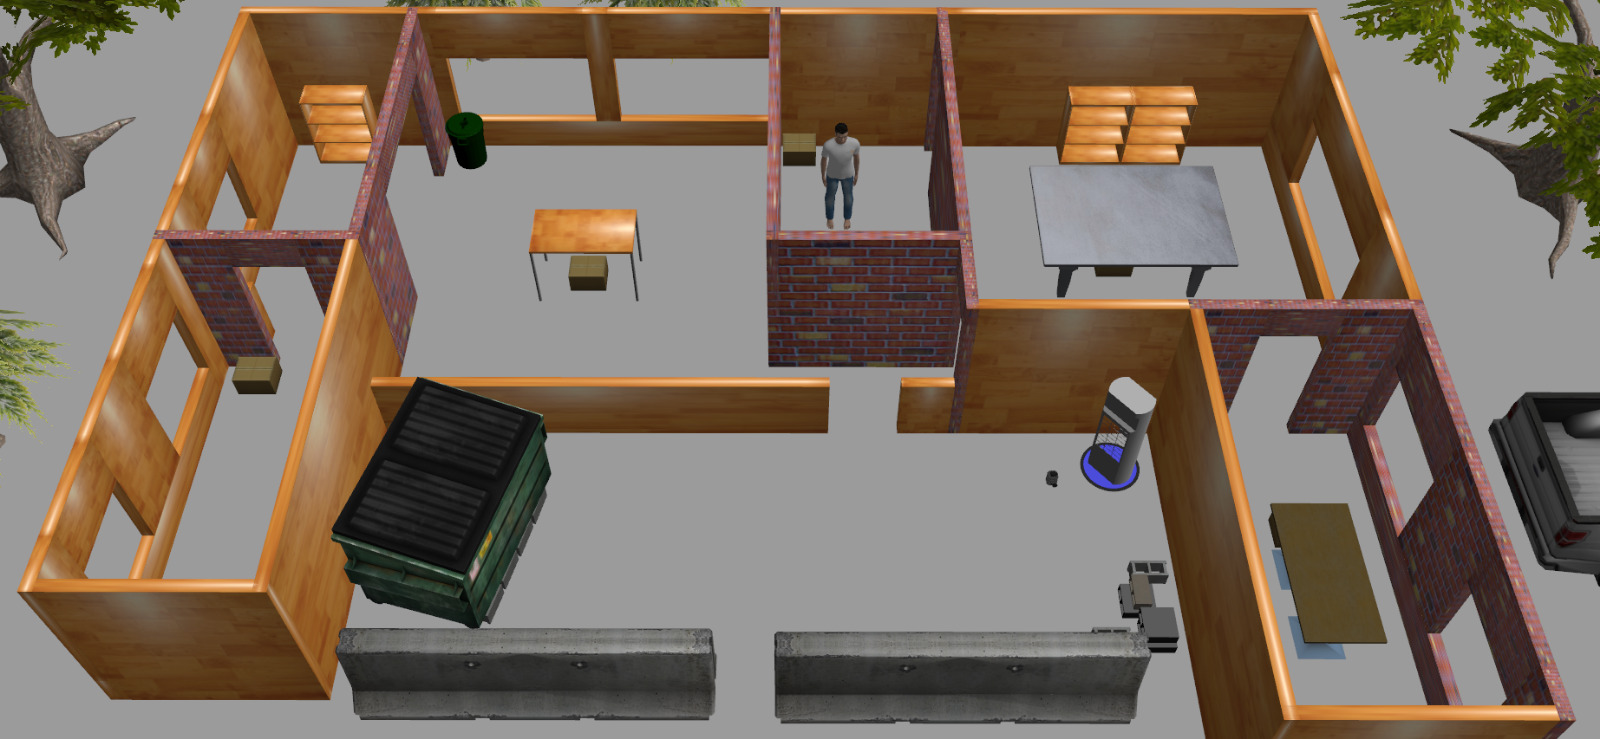
\includegraphics[width=0.8\linewidth]{RuntimeInfo-ICRA/figs/gazeboworld.jpeg}};
\end{tikzpicture}
    \caption{Path planning environment for a turtlebot (in blue) to infinitely often service a human (in red). The robot can recharge at a charging station (in green).}
    \label{fig:gazeboworld}
\end{figure}



We consider the \emph{runtime information} as a (possibly continuous) parameter associated with the environment. The work in~\cite{jangcontinuous} allows for near-optimal behaviour on continuous executions, however the authors focus on a specialized cost metric. Additionally, their method relies on online re-synthesis, which is not feasible for real-time deployment. This work was later extended in~\cite{Ehlerscost} to account for delay costs arising from a potentially adversarial environment. However, it relies on the discretization of the continuous parameter space, which fails to scale with the number of atomic propositions in the synthesis problem. 
In the service robot example, this information is a probability vector over possible human locations. In the UAM example, the information is the current incoming air traffic density. 

Our approach incorporates parametrized runtime information by switching between pre-computed strategies. First, for a given set of \emph{candidate instantiations} of the parameter we synthesize offline optimal strategies that satisfy all task specifications. Next, we obtain bounds on the suboptimality incurred by the use of these policies at \emph{all} other parameter values. This computation does not require discretization of the parameter space. At runtime, we dynamically switch strategies based on the these suboptimality bounds, thereby incorporating runtime information into the offline synthesis of correct-by construction policies. 
To this end, we derive a switching function that guarantees the resulting execution is provably correct, and near-optimal.

The main contributions detailed in this chapter are: 1) a novel switching protocol between pre-synthesized correct strategies that improves performance, 2) correctness of the switching protocol with respect to the mission specification, and 3) characterization of the suboptimality bounds on performance. We demonstrate the proposed approach on a motion planning problem for a service robot, and a traffic scheduling problem for UAM. 

%%%%%%%%%%%%%%%%%%%%%%%%%%%%%%%%%%%%%%%%%%%%%%%%%%%%%%%%%%%%%%%%%%%%%%%%%%%%%%%%%%%%%%%%%

\section{Preliminaries}\label{sec_prel}

\begin{figure*}[t!]
\centering
    \subfloat[$\overline{p}_1 = \lbrack1,0,0\rbrack $ \label{fig:gazebopolicies1}]{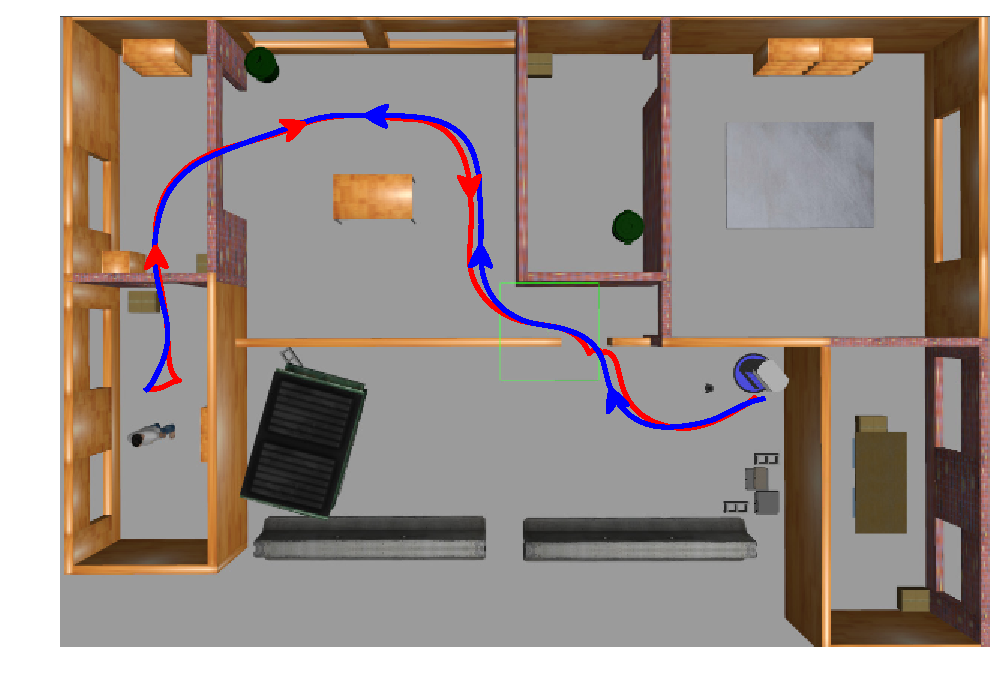
\includegraphics[width=0.33\linewidth]{RuntimeInfo-ICRA/figs/trivialtraj1.eps}}
    \subfloat[$\overline{p}_2= \lbrack0,1,0\rbrack $]{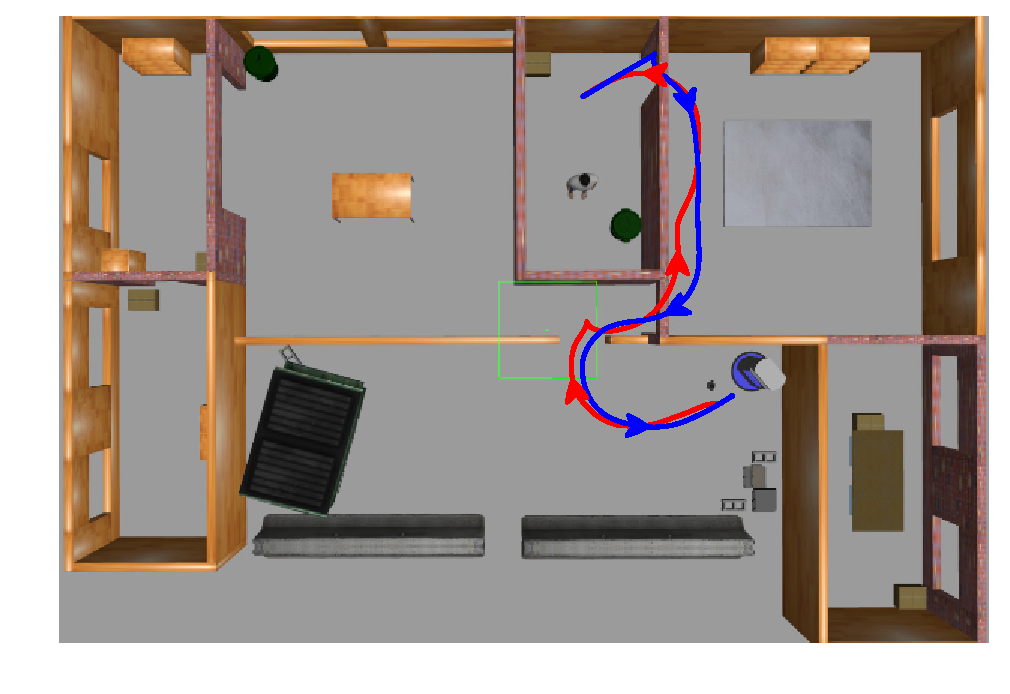
\includegraphics[width=0.33\linewidth]{RuntimeInfo-ICRA/figs/trivialtraj2.eps}}
    \subfloat[$\overline{p}_3 = \lbrack0,0,1\rbrack $]{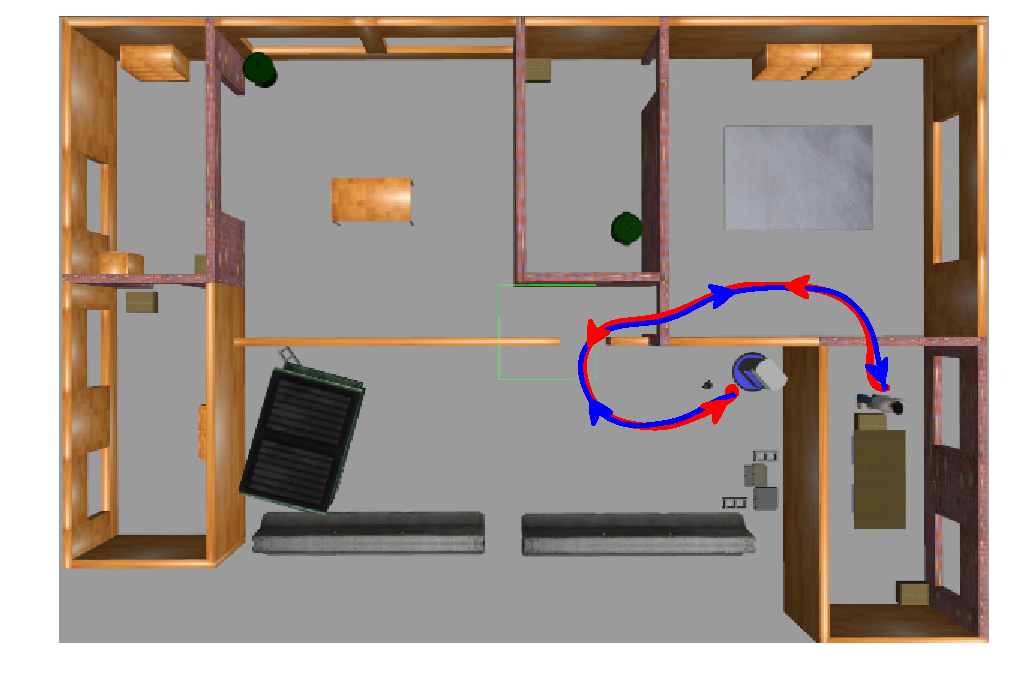
\includegraphics[width=0.33\linewidth]{RuntimeInfo-ICRA/figs/trivialtraj3.eps}}
    \caption{Continuous trajectories resulting from executing policies corresponding to the solution of~\eqref{prob:opt} for three different instantiations of runtime information vector $\overline{p} \colon \overline{p}_1 = [1,0,0]$, $\overline{p}_2 = [0,1,0]$, and $\overline{p}_3 = [0,0,1]$ .}\label{fig:trivialtrajs}
\end{figure*}

\subsubsection{Basic notation}
%
We consider reactive systems with a finite set $\inp$ of Boolean \emph{inputs}, controlled by the \emph{E}nvironment, and a finite set $\out$ of Boolean \emph{ outputs}, controlled by the \emph{A}gent. Together, they define the system's input alphabet $\ialphabet=2^\inp$ and the output alphabet $\oalphabet=2^\out$. We define $\alphabet=\ialphabet \times \oalphabet$. 

\subsubsection{\textbf{Game structures}}
%
We model the interaction between the agent and its environment as a two-player game. Formally, the game is played on a \emph{game structure} which is a tuple 
$\game = (\gstates, \ginit, \alphabet, \delta)$,
where:
\begin{itemize}
\item $\gstates$ is a finite set of states and $\ginit \in \gstates$ the initial state;
\item $\alphabet = \ialphabet \times \oalphabet$ is the alphabet of actions available to the environment and the agent respectively;
\item $\delta: \gstates \times \alphabet \rightarrow \gstates$
is a complete transition function, that maps each state, input (environment action) and output (agent action) to a successor state.
\end{itemize}

  

\subsubsection{Winning conditions}
%
The \emph{winning condition} for the agent in a game $\game$ is given as a set of plays $\varphi \subseteq \plays(\game)$ that specifies the set of plays that result in the agent winning the game. We consider games in which the agent has a \emph{Generalized Reactivity 1} (GR(1)) winning condition, which are common in a variety of practical applications. In the following, we make use of the linear temporal logic (LTL) operators \emph{always} $\LTLglobally$ and \emph{eventually} $\LTLfinally$. For full details on LTL syntax and semantics, we refer the reader to~\cite{MCBook}.

A GR(1) winning condition is defined by sets of states $S_\inp, S_\out \subseteq G$, $E_i \subseteq G$ for $i=1,\ldots,m$ and $F_j \subseteq G$ for $j=1,\ldots,n$, and consists of all plays $\overline \pi$ such that if $\overline{\pi} \in \LTLglobally S_\inp \cap \LTLglobally\,\LTLfinally\, E_{i}$ for all $i=1,\ldots,m$, then $\overline{\pi} \in \LTLglobally S_\out \cap \LTLglobally\,\LTLfinally\, F_{j}$ for all $j=1,\ldots,n$. Intuitively, for a play $\overline \pi$ to be winning, whenever the environment satisfies the assumptions $\LTLglobally\, S_\inp,\LTLglobally\,\LTLfinally\, E_{1},\ldots,\LTLglobally\,\LTLfinally\, E_{m}$, then the agent must satisfy all the guarantees $\LTLglobally\, S_\out,\LTLglobally\,\LTLfinally\, F_{j},\ldots,\LTLglobally\,\LTLfinally\, F_{n}$. By abuse of logical operators, we abbreviate GR(1)  conditions as
$$\varphi =  \left(\LTLglobally\, S_\inp \wedge \bigwedge_{i=1}^{m}  \LTLglobally\,\LTLfinally\, E_{i}\right) \rightarrow
\left(\LTLglobally\, S_\out \wedge \bigwedge_{i=1}^{n} \LTLglobally\,\LTLfinally\,F_{i}\right).$$


\subsubsection{Strategies}
%
A \emph{strategy for the agent} is a function $\rho_\out:
\prefs(\game) \times \ialphabet \rightarrow
\oalphabet$ which maps a prefix (the history of the play so far) and an action of the environment to an action of the agent. 
A \emph{strategy for the environment} is a function $\rho_\inp: \prefs(\game)\rightarrow \ialphabet$ that maps the prefix of the play so far to an action of the environment. We denote the sets of all strategies for the agent and for the environment by $\mathcal{M}_\out $ and $\mathcal{M}_\inp$ respectively.

Every pair of strategies $\rho_\out \in \mathcal{M}_\out$ for the agent and $\rho_\inp \in \mathcal{M}_\inp$ for the environment define a play, denoted by $\Pi(\rho_\out,\rho_\in)$. More precisely,  
$\Pi(\rho_\out,\rho_\in) = \overline{\pi} = (g_0,\symb_{\inp,0},\symb_{\out,0}, g_1) 
(g_1,\symb_{\inp,1}, \symb_{\out,1}, g_2) \ldots \in \plays(\game)$
where
for every $i \geq 0$, $\symb_{\inp,i} = \rho_\inp(\overline\pi[0,i])$ and $\symb_{\out,i} = \rho_\out(\overline\pi[0,i],\symb_{\inp,i})$.
Similarly, we define the set of plays starting at a state $g$ that are consistent with $\rho_\out$, denoted $\plays(\game,\rho_\out,g)$.

Given a game structure $\game$ and a winning condition $\varphi$ for the agent, we seek to synthesize a strategy $\rho_\out\in \mathcal{M}_\out$ for the agent such that for every strategy $\rho_\inp \in \mathcal{M}_\inp$ for the environment it holds that $\Pi(\rho_\inp,\rho_\out) \in \varphi$, i.e., all resulting plays satisfy $\varphi$.
In such cases we say that \emph{$\rho_\out$ satisfies $\spec$}, denoted $\rho_\out\models\spec$.








%%%%%%%%%%%%%%%%%%%%%%%%%%%%%%%%%%%%%%%%%%%%%%%%%%%%%%%%%%%%%%%%%%%%%%%%%%%%%%%%%%%%%%%%%

\section{Problem formulation}\label{sec:prob}

We represent \emph{runtime information} as $n$-dimensional real vectors, for a given $n \in \mathbb N$. We denote the set of all possible vector values for the runtime information by $\mathcal{P}\subseteq \mathbb{R}^n$. We score the performance of each play in the game using runtime information in $\mathcal{P}$ via a performance metric, $J: \plays(\game)\times\mathcal{P} \to \mathbb{R}$. 


% \begin{itshape}
% \textbf{Example.} Consider Figure~\ref{fig:gazeboworld}, where the robot has to infinitely often find a human. In this case, the runtime information $\overline{p} \in\mathbb{R}^8$ is a probability vector that represents the likelihood of a human being in each particular room. The set $\mathcal{P}=\{\overline{p}\in \mathbb{R}^8: \overline{p}\succeq 0, \overline{1}^\top\overline{p}=1\}$ is the probability simplex, with $\overline{1}$ as a vector of ones.
% \label{ex:toy_ex}
% \end{itshape}


\subsubsection*{Assumption}
For every $\overline p \in \mathcal{P}$ and every strategy $\rho_\out\in\mathcal{M}_\out$ such that $\rho_\out\models\spec$, there exists a strategy $\rho_\inp \in\mathcal{M}_\inp$ such that $  J(\Pi(\rho_\out,\rho_\inp), \overline p) \geq J(\Pi(\rho_\out,\rho_\inp'), \overline p)$ for every $\rho_\inp'\in\mathcal{M}_\inp$. 

The above assumption ensures a well-defined cost function using the metric $J$. We can thus define
\begin{align}
C(\rho_\out,\overline{p}) = max_{\rho_\inp \in\mathcal{M}_\inp}J(\Pi(\rho_\out,\rho_\inp), \overline p)
\end{align}
as the cost function, with $C:\Sigma_\out \times \mathcal{P} \to \mathbb{R}$.
% Under the above assumption, we can associate a cost value with each strategy $\rho_\out$ for the agent, and each instance of the runtime information $\overline p$:
%In general, $\overline{p}$ serves as a way to introduce
%additional information at runtime. We are interested in
%using this information gained at runtime in order to act
%more optimally. We thus introduce a notion of being
%\emph{optimal with respect to this runtime information}. 
Given the runtime information $\overline p \in \mathcal P$, a strategy $\rho_\out \in \mathcal M_\out$ for the agent that satisfies $\spec$ is \emph{optimal for $\overline p$} if and only if it is a solution to the following optimization problem.
\begin{align}
    \begin{array}{rl}
        \underset{\rho_\out\in
        \mathcal{M}_\out}{\mathrm{minimize}}&\quad
        \ \\
        \mathrm{subject\ to}&\quad \rho_\out\models \varphi
    \end{array}\label{prob:opt}%
\end{align}
Let $C^\ast: \mathcal{P} \to \mathbb{R}$ denote the optimal value of \eqref{prob:opt}.

% \begin{example}[]
\begin{itshape}
\textbf{Example.} Consider Figure~\ref{fig:gazeboworld}, where the robot has to infinitely often meet the human. Assume that the human can only be in rooms $R_1, R_4, R_8$. Let $q_1,q_2,q_3\in[0,1]$ be the probabilities of the human being in room $R_1$, $R_4$ and $R_8$ respectively. The runtime information is $\overline{p}= {[q_1\ q_2\ q_3]}^\top \in\mathcal{P}\subseteq \mathbb{R}^3$, where the set $\mathcal{P}$ is the probability simplex. The cost function is, 
\begin{align}
C(\rho_\out, \overline{p}) &= \mathbb E\lbrack\text{time to find human\rbrack}= \sum\nolimits_{i=1}^N T_i(\rho_\out)\, q_i\label{eq:cost_fun}
\end{align}
where $T_i$ is the time taken to reach room $i$ under the robot strategy $\rho_\out$. Figure \ref{fig:trivialtrajs} shows the resulting continuous trajectories from executing policies when the information vector tells the robot the exact room occupied by the human. \label{ex:toy_ex2}
\end{itshape}
% \end{example}


Information is only provided at runtime and the agent has no control over its value. One method to guarantee optimality with respect to the runtime information is to directly incorporate $\overline{p}$ into the state as an additional environment variable and solve \eqref{prob:opt} for all possible values for $\overline{p}$. Such an approach would fall under the framework presented in \cite{Ehlerscost}. However, if $\overline{p}$ is continuous, this requires discretization which can blow up the state-space. In Example \ref{ex:toy_ex2}, we can easily find a discretization of $p$ to guarantee optimality without a state-space explosion, however, this is not true in general.

Another approach is to re-synthesize online when the value of $\overline{p}$ changes. Such an approach requires re-solving \eqref{prob:opt} at every instant $\overline{p}$ changes. However, the computational effort required to solve \eqref{prob:opt} is prohibitively high for an on-board deployment. Hence, we propose pre-synthesizing offline a set of \emph{representative strategies} for specific instantiations of $\overline{p}$.

Given a set of representative strategies associated with instances of the runtime information, the task at runtime then becomes one of choosing a strategy depending on the current value of $\overline p$. As we have a finite set of strategies to choose from, the resulting behaviour of the agent will be \emph{approximately optimal}. Thus, we consider the problem of synthesizing an \emph{approximately optimal switching function} that also guarantees $\spec$.

\begin{defn}
Given a game structure $\game$ and a set of strategies $\{{\rho_\out}_i\in \mathcal{M}_\out\}_{i=1}^N$ for the agent, a \emph{switching function} is a function $\tau : \prefs(\game) \times \mathcal P^* \to \{1,\ldots,N\}$, which maps a play prefix and the sequence of values of $\overline p$ seen so far, to an index of a strategy in the given set.

The set of plays resulting from applying the switching function $\tau$ to $\{{\rho_\out}_i\in \mathcal{M}_\out\}_{i=1}^{N}$ is defined as the set of plays 
$\plays(\{{\rho_\out}_i\in\mathcal{M}_\out\}_{i=1}^{N},\tau)$ such that 
$\overline{\pi} = (g_0,\symb_{\inp,0},\symb_{\out,0}, g_1) 
(g_1,\symb_{\inp,1}, \symb_{\out,1}, g_2) \ldots \in \plays(\{{\rho_\out}_i\in \mathcal{M}_\out\}_{i=1}^{N},\tau)$
if and only if there exists $\overline \gamma \in \mathcal{P}^\omega$ such that
for every $i \geq 0$,  it holds that $\symb_{\out,i} ={\rho_\out}_{\tau(\overline \pi[0,i],\overline \gamma[0,i])}(\pi[0,i],\symb_{\inp,i})$.
\end{defn}

Informally, we want to be able to \emph{switch} between pre-computed strategies based on values of the runtime information. In order to not violate the specification, switching needs to take into account the prefix of the play. We formalize this task below. 

   We are given a game $(\game,\varphi)$, 
   a set $\{\overline{p}_i\in \mathcal{P}\}_{i=1}^{N}$ of representative values of the runtime information, and 
    strategies $\{{\rho_\out^\ast}_i\in \mathcal{M}_\out\}_{i=1}^{N}$ such that ${\rho_\out^\ast}_i$ solves \eqref{prob:opt} for $\overline{p}_i$. Given $\epsilon > 0$, compute a collection $\{\mathcal S_i\}_{i=1}^N$ of subsets of $\mathbb{R}^n$ such that $\overline{p}_i \in \mathcal{S}_i$, and a  switching function $\tau : \prefs(\game) \times \mathcal P^+ \to \{1,\ldots,N\}$ that satisfies the following conditions.
   \begin{itemize}
       \item For all $i =1,\ldots,N$ and all $\overline p \in \mathcal S_i \cap \mathcal P$ it holds that
    \begin{align}
  C({\rho_\out}_i^\ast,
    \overline{p}) - \epsilon \leq
        C^\ast(\overline{p}) \leq
        C({\rho_\out}_i^\ast,
    \overline{p}).
    \label{eq:bounds}
   \end{align}  
   \item $\overline\pi \in \varphi$ for every play $\overline \pi \in \plays(\{{\rho_\out}_i\in\mathcal{M}_\out\}_{i=1}^{N},\tau)$.
   \end{itemize}


 In the next Section we discuss how to compute, using off-the-shelf synthesis methods, representative strategies that are \emph{correct}, that is, they satisfy $\spec$, and optimal for a given runtime information vector $\overline{p}$.

 Then, we provide a method for computing a switching function
 for the synthesized representative strategies that is also guaranteed to be \emph{correct}, and is approximately optimal with respect to suitably chosen lower and upper bound functions $L$ and $U$. As formalized previously, correctness means that every play resulting from applying the switching function to the given strategies satisfies the specification $\spec$. Approximate optimally is with respect to the optimal value $C^\ast(\overline{p})$ for each runtime information value $\overline{p} \in \mathcal P$.

% In Section~\ref{sec:synth_strats}, we show how to
% synthesize representative strategies that are \emph{correct}, that is, they satisfy $\spec$, and optimal for a given runtime information vector $\overline{p}$. 

% In Section \ref{sec:gen_strats} we provide a method for computing a switching strategy 
% for the synthesized representative strategies that is also guaranteed to be \emph{correct}, and is approximately optimal with respect to suitably chosen lower and upper bound functions $L$ and $U$.

%However, while we guarantee that the chosen strategies dominates the other pre-specified strategies, we cannot guarantee that, for a given $\epsilon$ and $\overline{p}$, the chosen strategy is $\epsilon-$optimal. We will thus also present an iterative procedure to generate more strategies offline that will guarantee, under certain conditions, that the chosen strategy will always be $\epsilon-$optimal for any $\overline{p}$. 


%%%%%%%%%%%%%%%%%%%%%%%%%%%%%%%%%%%%%%%%%%%%%%%%%%%%%%%%%%%%%%%%%%%%%%%%%%%%%%%%%%%%%%%%%

\section{Synthesis of correct-by-construction strategies with near-optimality guarantees}

We constuct a switching function that guarantees that the resulting plays satisfy the task specification $\spec$. We also provide suboptimality bounds for the performance when using the proposed method. We utilize existing synthesis techniques~\cite{Ehlerscost} to synthesize for each $i \in \{1,\ldots,N\}$ a strategy that is \emph{correct}, i.e., satisfies $\spec$, and optimal for the specific $\overline{p}_i$.

\subsection{Suboptimality bounds for unknown runtime information}
\label{sec:generalization}
Let $\{\overline{p}_i\in \mathcal{P}\}^{N}_{i=1}$ be the given candidate instantiations of the runtime information, and let 
$\{{\rho_\out^\ast}_i\in \mathcal{M}_\out\}_{i=1}^{N}$ be the corresponding optimal strategies. That is, for each $i$, ${\rho_\out}_i^\ast$ is an optimal solution of \eqref{prob:opt} for $\overline{p}_i$. 
Under Assumption~\ref{assum:C_lin} below, we can compute a collection of polytopes ${\{\mathcal{S}_i\}}_{i=1}^N$ such that ${\rho_\out^\ast}_i$ is $\epsilon$-optimal, whenever $\overline p \in \mathcal{S}_i$.
\subsubsection*{Assumption}\label{assum:C_lin}
  The cost function $C: \mathcal M_\out\times \mathcal{P}
  \to \mathbb{R}$ is such that for all $\rho_\out \in \mathcal M_\out$ and $\overline p = {[q_1\ q_2\ \ldots\ q_n]}^\top \in \mathcal P \subseteq \mathbb{R}^n$:
  \begin{align}
        C(\rho_\out, \overline{p}) = \sum_{i=1}^n
        C(\rho_\out, \overline{e}_i)\, q_i,\label{eq:V_lin_decompose}
    \end{align}
    where $\overline{e}_i$ is the vector that has $1$ at
     position $i$ and $0$ elsewhere.


We address Problem~\ref{prob_st:main} by defining a collection of polytopes $\{\mathcal{S}_i\}_{i=1}^N$, where $\mathcal{S}_i= \{ \overline{p} \in \mathbb{R}^n \mid H_i \overline{p}\leq
\overline{b}_i\}$ and
{\small\begin{align}
    H_i &= \left[
        \begin{array}{ccc}
            C({\rho_\out}_i^\ast, \overline{e}_1) -
            C({\rho_\out}_1^\ast, \overline{e}_1) &
            \cdots &
            C({\rho_\out}_i^\ast, \overline{e}_n) -
            C({\rho_\out}_1^\ast, \overline{e}_n)\\
            C({\rho_\out}_i^\ast, \overline{e}_1) -
            C({\rho_\out}_2^\ast, \overline{e}_1) &
            \cdots &
            C({\rho_\out}_i^\ast, \overline{e}_n) -
            C({\rho_\out}_2^\ast, \overline{e}_n)\\
            \vdots & \vdots & \vdots \\
            C({\rho_\out}_i^\ast, \overline{e}_1) -
            C({\rho_\out}_N^\ast, \overline{e}_1) &
            \cdots &
            C({\rho_\out}_i^\ast, \overline{e}_n) -
            C({\rho_\out}_N^\ast, \overline{e}_n)\\
            C({\rho_\out}_i^\ast, \overline{e}_1) -
            C^\ast(\overline{e}_1) &
            \cdots &
            C({\rho_\out}_i^\ast, \overline{e}_n) -
            C^\ast(\overline{e}_n)
    \end{array}\right] \label{eq:A_defn} \\
        \overline{b}_i&={[0\ 0\ \ldots\ 0\
        \epsilon]}^\top\in \mathbb{R}^{N+1}\label{eq:b_defn}
\end{align}}\normalsize%
with $H_i\in \mathbb{R}^{(N+1)\times n}$. By \eqref{prob:opt} and Assumption~\ref{assum:C_lin}, we have the following upper bound on $C^\ast(\overline{p})$ for any runtime information vector $ \overline{p}={[q_1\ q_2\ \ldots\ q_n]}^\top\in
\mathcal{P}$,
\begin{align}
    C^\ast( \overline{p})\leq
    C({\rho_\out}_i^\ast,
    \overline{p})=\sum_{j=1}^nC({\rho_\out}_i^\ast,
    \overline{e}_j)q_j\label{eq:C_ub},\quad \forall
    i\in\{1,\ldots,N\}.
\end{align}

Theorem~\ref{thm:bounds} below ensures that using ${\rho_\out^\ast}_i$ for vectors $\overline p \in \mathcal{S}_i$ results in $\epsilon$-optimal performance, provided the polytopes $\mathcal{S}_i$ are non-empty. In other words, the difference between $C^\ast(\overline p)$, the optimal performance for a runtime information $\overline{p}$,  and $C(\rho_{\out_i}^\ast, \overline p)$, the attained performance due to choice of strategy $\rho_{\out_i}^\ast$,  can not be larger than $\epsilon$, whenever $\overline p \in \mathcal{S}_i$. To complete the discussion, we provide a sufficient condition for non-empty polytopes $\mathcal{S}_i$ in Proposition~\ref{prop:nonempty}.
 
\begin{thm}\label{thm:bounds}
    Let the polytopes $\mathcal{S}_i$ be non-empty. Given runtime information $ \overline{p} \in \mathbb{R}^n$,
    if $ \overline{p}\in \mathcal{S}_i$ for some
    $i\in\{1,\ldots, N\}$, then
    \begin{align}
        C({\rho_\out}_i^\ast,
    \overline{p}) - \epsilon \leq
        C^\ast(\overline{p}) \leq
        C({\rho_\out}_i^\ast,
    \overline{p}). \nonumber
    \end{align}
\end{thm}
\begin{proof}
   The upper bound on $C^\ast( \overline{p})$ follows from
   \eqref{eq:C_ub}. Consider the collection of polytopes $
    \mathcal{T}_i$ constructed using the first $N$
    hyperplanes in \eqref{eq:A_defn} and \eqref{eq:b_defn}.
    For every $ \overline{p}\in \mathcal{T}_i$,
    % ={[q_1\ %q_2\ \ldots\ q_n]}^\top\in \mathcal{T}_i\subset \mathbb{R}^n$,
    \begin{align}
        %\sum_{j=1}^nC(\overline{\gamma}_i^\ast,
        %\overline{e}_j) q_j&\leq
        %\sum_{j=1}^nC(\overline{\gamma}_k^\ast,
        %\overline{e}_j)q_j,\ \forall
        %k\in\{1,\ldots,N\}\setminus\{i\}\label{eq:dom}.
        C({\rho_\out}_i^\ast, \overline{p})&\leq
        C({\rho_\out}_k^\ast, \overline{p}),\ \forall
        k\in\{1,\ldots,N\}\setminus\{i\}\label{eq:dom}.
    \end{align}
    In other words, among the $N$  strategies
    ${\rho_\out}_{(\cdot)}^\ast$,
    ${\rho_\out}_{i}^\ast$ provides the tightest upper
    bound on $C^\ast( \overline{p})$ due to \eqref{eq:C_ub}. 
    
   
   We next prove the lower bound. The last
   hyperplane in \eqref{eq:A_defn} and \eqref{eq:b_defn}
   guarantees that $ C(
   {\rho_\out}_i^\ast, \overline{p}) -  \overline{\ell}^\top \overline{p} \leq \epsilon$ for
   every $ \overline{p}\in \mathcal{S}_i$, where $\overline{\ell}_j = C^\ast( \overline{e}_j)$. On adding and
   subtracting $C^\ast( \overline{p})$, we have
   $C({\rho_\out}_i^\ast, \overline{p}) - C^\ast(
   \overline{p}) + C^\ast(\overline{p}) -
   \overline{\ell}^\top \overline{p} \leq \epsilon$. Since
   $C( \cdot, \overline{e}_j)\geq \ell_j$ by definition of $
   \overline{\ell}$, we have $C^\ast(\overline{p}) -
   \overline{\ell}^\top \overline{p} \geq 0$ for every $
   \overline{p}\in \mathcal{S}_j$. Therefore, $C({\rho_\out}_i^\ast, \overline{p}) - C^\ast(
   \overline{p}) \leq \epsilon$.
\end{proof}
\begin{prop}\label{prop:nonempty}
    Let Assumption~\ref{assum:C_lin} hold. For every $i=1,\ldots,N$ the polytope $\mathcal{S}_i$ is non-empty, provided that $\epsilon \geq \max_i\left\{ C( {\rho_\out}_i^\ast, \overline{p}_i) -
    \overline{\ell}^\top \overline{p}_i\right\}$. Here,
    $\overline{\ell}={[C^\ast( \overline{e}_1)\ C^\ast(\overline{e}_2)\ \ldots\ C^\ast( \overline{e}_n)]}^\top\in \mathbb{R}^n$.
    % Moreover, each of the pairwise-intersections of the polytopes is either a hyperplane or is the empty set.
\end{prop}
\begin{proof}
    The polytopes $ \mathcal{T}_i$ (defined in the proof of Theorem~\ref{thm:bounds}) are non-empty, since they
    contain $ \overline{p}_i$ by the optimality of $
    {\rho_\out}_i^\ast$ in \eqref{prob:opt}.
    The last hyperplane in \eqref{eq:A_defn} and
    \eqref{eq:b_defn} is also satisfied by $
    \overline{p}_i$, thanks to the use of $\epsilon$ in $\overline b_i$.
    Thus, its intersection with $ \mathcal{T}_i$, which
    yields the polytope $ \mathcal{S}_i$, is non-empty.
    % By construction, the
    % pairwise-intersection of the polytopes $ \mathcal{T}_i$
    % are either hyperplanes (overlapping boundary of
    % $\mathcal{T}_i$ and $\mathcal{T}_k,\ k\neq i$) or empty. 
\end{proof}


\subsection{Switching function construction}\label{sec:switching}
In order to guarantee that the plays resulting from switching between the synthesized representative strategies satisfy the specification $\spec$, the switching function needs to keep track the satisfaction of the agent's liveness guarantees $\LTLglobally\LTLfinally F_i$ in $\spec$. Since the cost function $C$ captures the cost of achieving the liveness guarantees, when the specification is satisfied due to a violation of the environment assumptions, no switching would be necessary, as the cost would be $0$.

To ensure that the switching between strategies does not prevent the agent from infinitely often visiting each of the sets $F_i$, the switching function will keep track of these visits, and only allow switching to a different strategy once all the sets $F_i$ have been visited under the current strategy. Furthermore, the switch can only occur from a state from which the next strategy can guarantee the satisfaction of $\spec$. Below we make this intuition precise by providing the construction of the switching function as a finite-state system.

Let $\{{\rho_\out^\ast}_i\in \mathcal{M}_\out\}_{i=1}^{N}$ be a set of strategies  for the agent such that ${\rho_\out}_i^\ast \models \spec$ for each $i \in \{1,\ldots,N\}$, and let $\{\mathcal S_i\}_{i=1}^N$ be the polytopes computed as in Section~\ref{sec:generalization}.

For each ${\rho_\out^\ast}_i$, let $W_i = \{g\in G \mid \plays(\game,{\rho_\out^\ast}_i,g)\subseteq \spec\}$ denote the set of states from which the specification can be enforced by following the strategy ${\rho_\out^\ast}_i$.

We define a finite state transition system with states $Q$, initial state $q_0$, transition function $\theta$ and alphabet $(G \times \ialphabet \times \oalphabet \times G) \times \{\mathcal S\}_{i=1}^N$. The set of states is $Q = \{ V \mid V \subseteq \{1,\ldots, n\}\} \times \{1,\ldots,N\}$, where $n$ is the number of liveness guarantees in $\spec$. States in $Q$ track the guarantees that have been satisfied and contain the index of the currently chosen strategy. The initial state is $q_0 = (\{1,\ldots,n\},1)$. The transition function $\theta : Q \times ((G \times \ialphabet \times \oalphabet \times G) \times \{\mathcal S\}_{i=1}^N) \to Q$ is defined such that 
$\theta((V,i),((g,\symb_{\inp}, \symb_{\out}, g'),\mathcal S)) = (V',i')$, where
\begin{itemize}
\item if $V = \{1,\ldots,n\}, \mathcal S = \mathcal S_{j}, g' \in W_{j}$, then, $V' = \emptyset, i'=j$,
\item $V' = V \cup \{j \in \{1,\ldots,n\} \mid g \in F_j\}$ and $i'=i$ otherwise.
\end{itemize}
That is, once all the sets $F_j$ have been visited under the current strategy, we can switch to the $i'$-th strategy and reset the tracking set to $\emptyset$. Otherwise we record the indices of the visited sets and keep the strategy index the same. We can extend $\theta$ to words in the usual way. 

We define the switching function such that 
$\tau (\varepsilon,\overline p_0) = \min(\{i \mid p_0 \in \mathcal S_i\}\cup \{N\})$, where $\varepsilon$ is the empty word, and for every 
$\overline \pi =(g_0,\symb_{\inp,0},\symb_{\out,0}, g_1) \ldots
(g_k,\symb_{\inp,k}, \symb_{\out,k}, g_{k+1})$ and every $\overline \gamma = \overline p_0\ldots\overline p_{k+1}$ we let
$\tau (\overline \pi, \overline\gamma) = i$ where
$\theta(((g_0,\symb_{\inp,0},\symb_{\out,0}, g_1),\mathcal S_{i_1}) \ldots
((g_k,\symb_{\inp,k}, \symb_{\out,k}, g_{k+1}),\mathcal S_{i_{k+1}})) = (V,i)$ for some $V$, where for all $j\geq 1$ we have $i_j  = \min(\{i \mid \overline p_j \in \mathcal S_i\text{ and }g_j \in W_{i_j}\} \cup \{N\})$.

As the switching function $\tau$ only allows switching to a different strategy once all $F_j$ have been visited under the current strategy, this means that if we switch strategy infinitely often then the liveness guarantee is satisfied. If, on the other hand, we stabilize at some strategy, $\spec$ is again guaranteed by the fact that this strategy satisfies the specification. 


\subsection{Discussion}
The key advantage of our approach is that we avoid the re-synthesis of strategies for each new value of the runtime information, when the parameter set is covered by the collection of polytopes ${\{\mathcal{S}_i\}}_{i=1}^N$,  $\mathcal{P}\subseteq\cup_{i=1}^N \mathcal{S}_i$.  We also avoid discretization of the set $\mathcal{P}$. This enables on-board deployment of our approach with guaranteed $\epsilon$-optimal performance. In contrast, traditional approaches rely either on re-synthesis or on discretization of the parameter space which requires either prohibitively high computational or memory costs~\cite{jangcontinuous,smith2011optimal}. When $\mathcal{P}\not\subseteq\cup_{i=1}^N \mathcal{S}_i$, none of the synthesized strategies guarantees $\epsilon$-optimal performance for the parameter values in $\mathcal{P}\setminus\cup_{i=1}^N \mathcal{S}_i$. In such cases, we can iteratively expand the candidate instantiations offline till the entire parameter space $\mathcal{P}$ is covered. Specifically, we add to the candidate instantiations randomly chosen parameter values in $\mathcal{P}\setminus\cup_{i=1}^N \mathcal{S}_i$. In future, we intend to investigate sufficient conditions under which such an expansion approach terminates in finite number of steps.



% 1. Discussion of the partition not being complete. Why we can't do state augmentation with the parameter?
% 2. All bets are off if the information vector is incorrect.
%From Proposition~\ref{prop:nonempty}, the
%collection of polytopes $\{\mathcal{S}_i\}$ forms an
%incomplete partition of $ \mathcal{P}$, i.e., it is possible that 
% $\mathcal{P}\not\subseteq\cup_{i=1}^n \mathcal{S}_i$.

% Alternatively, we can choose parameters greedily that provides the largest volume polytope $\mathcal{S}_{(\cdot)}$. Note that the second construction results in a submodular maximization problem over an uncountable set~\cite{}.

% Our approach implicitly assumes that the provided runtime information is correct. We expect our approach to exhibit suboptimal performance in problems with incorrect runtime information. We intend to investigate problems with false or misleading information in future. 

% By construction, the polytopes $\mathcal{S}_i$ are either mutually disjoint or intersect at a hyperplane. 

% As the additional information is only available during runtime, we would ideally synthesize a strategy that yields optimal behaviour for all instances of the vector $\overline p$. One way to achieve this is to include this information as an additional component of the input. Since, however, the input is discrete and the runtime information is real-valued this requires discretization, and, more importantly, can significantly increase the size of the problem instance. Another approach is to re-synthesize the strategy of the agent at runtime, that is, solve~\eqref{prob:opt} every time the value of $\overline{p}$ changes.
% However, the computational effort required to solve 

% Therefore, we propose a different approach. We first synthesize offline a set of \emph{representative strategies} that are \emph{optimal with respect to individual representative values of the runtime information}, and then combine them in a strategy that switches between the individual strategies based on the information received at runtime.

% \begin{itshape}\textbf{Example cont'd.}
% The robot only has enough charge to visit one of the three rooms and return to the charging station. Hence, knowing the likelihood of the human's location can greatly the reduce expected time to find them.  The optimal policy for each $p_i$ corresponds to an \emph{ordering} of which room to visit. Intuitively, the robot will visit rooms in decreasing order of likelihood of a human being there. 

% Consider again the example in Figure~\ref{fig:gazeboworld}. Assume we have three representative instantiations of the runtime information vector given by $\overline{p}_1 =\lbrack 0.6, 0.3, 0.1\rbrack$, $\overline{p}_2 = \lbrack 0.7, 0.2, 0.1\rbrack$, and $\overline{p}_3 = \lbrack 0.9, 0.07, 0.03\rbrack$. Intuitively, the optimal policy in each case is the same - the robot first visits $R_1$, then recharges in $R_7$, then visits $R_4$, recharges, and finally visits $R_8$.

% We see in Table~\ref{tab:examplesameroom}, that the same policy with the human in the same room results in different optimal values based on the current runtime information value.
% \end{itshape}
% \begin{table}[h]
%     \centering
%     \begin{tabular}{c|c|c}\toprule
%         $\mathbf{\overline{p}}$  & \textbf{Human location}  &  $\mathbf{C^\ast}$ \\ \midrule
%         $\lbrack 0.6, 0.3, 0.10\rbrack$ & $R_1$ & 11.1 \\
%         $\lbrack 0.7 ,0.2, 0.10\rbrack$ & $R_1$ & 10.4\\
%         $\lbrack 0.9, 0.1, 0.0\rbrack$ & $R_1$ & 7.9 \\ \bottomrule
%     \end{tabular}
%     \caption{Caption}
%     \label{tab:examplesameroom}
% \end{table}{}

% Hence, our cost metric captures acting optimally with respect to the current knowledge about the environment. In the case where we have no knowledge whatsoever (corresponding to a uniform probability distribution in the previous example), the cost metric is equivalent to those defined in \cite{Ehlerscost}. 




%%%%%%%%%%%%%%%%%%%%%%%%%%%%%%%%%%%%%%%%%%%%%%%%%%%%%%%%%%%%%%%%%%%%%%%%%%%%%%%%%%%%%%%%%

\section{Experiments}
All experiments we report on were performed on an Intel i5-5300U 2.30 GHz CPU with 8 GB of RAM.  We used the tool \texttt{Slugs}~\cite{Ehlerslugs} for the strategy synthesis. 

\subsection{Robot motion planning}

We consider the example discussed in Section~\ref{sec:prob} (Figure~\ref{fig:gazeboworld}).
Formally, the specification is
\[
    \varphi = \LTLglobally (h \in R_1 \cup R_4 \cup R_8) \rightarrow \Big( \LTLglobally \LTLfinally (r = h) \wedge \LTLglobally (\mathrm{Energy} > 0) \Big),
\]
where $h$ and $r$ are variables modelling the human and robot positions respectively, and $\mathrm{Energy}$ is the robot's energy level.
The cost function $C(\cdot)$ is given in \eqref{eq:cost_fun}.
The runtime information $\overline{p}$ is the probability distribution over the human's possible locations - $R_1, R_4,R_8$. 
In our experiments, we used a Bayesian update to compute $\overline{p}$ using the current (and past) observations of the human's position. 

\begin{table}
    \centering
    \begin{tabular}{|c|c|c|c|c|}\toprule
        Query point  & \multirow{2}{*}{Strategy} & \multicolumn{3}{c|}{Cost}  \\\cmidrule{3-5}
        $\overline{p}$  & & L. bound & U. bound &  $C^\ast(\overline{p})$\\  \midrule
        $[0.1, 0.8, 0.1]$ & $\rho_{\out_2}$ & 7.19 & 10.4 & 9.5 \\ 
        $[0.0, 0.1, 0.9]$ & $\rho_{\out_3}$  & 6.39 & 9.6 & 7.9 \\ 
        \rowcolor{red!10} $[0.6, 0.3, 0.1]$ & -- & -- & -- & 11.1\\ \bottomrule
    \end{tabular}
    \caption{Lower and upper bounds (Theorem~\ref{thm:bounds}) and the optimal value $C^\ast(\overline{p})$ for some runtime information vectors $\overline{p}$.}
    % (lower $C^\ast(\rho_{\out_{i}}^\ast,\overline{p})-\epsilon$ and upper $C^\ast(\rho_{\out_{i}}^\ast,\overline{p})$)
    \label{tab:perf}
\end{table}{}
\begin{figure}
    \centering
    % This file was created by matlab2tikz.
%
%The latest updates can be retrieved from
%  http://www.mathworks.com/matlabcentral/fileexchange/22022-matlab2tikz-matlab2tikz
%where you can also make suggestions and rate matlab2tikz.
%
\definecolor{mycolor1}{rgb}{1.00000,0.00000,1.00000}%
\definecolor{mycolor2}{rgb}{0.00000,1.00000,1.00000}%
%
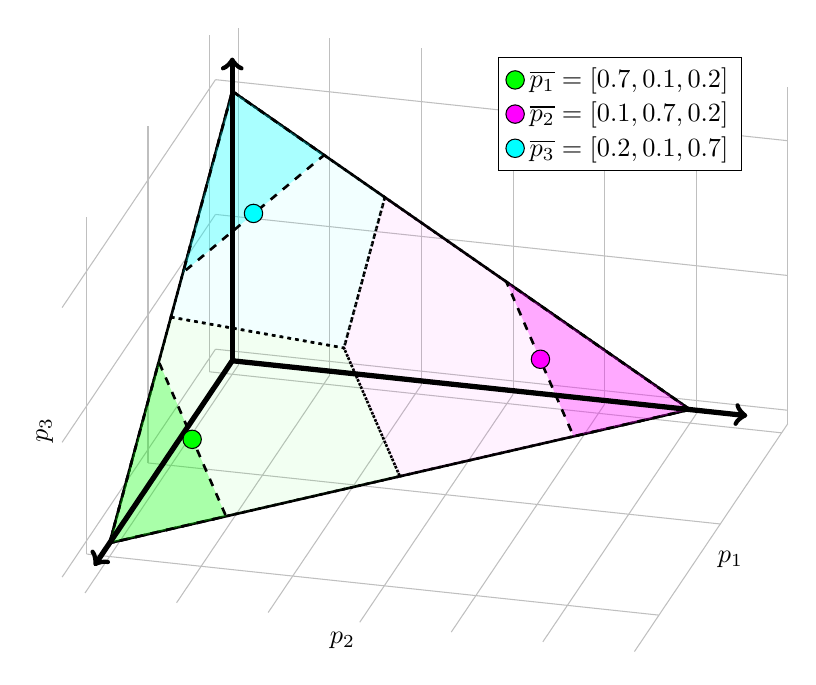
\begin{tikzpicture}[scale=0.95]

\begin{axis}[%
% width=6.396in,
width=0.8\linewidth,
% height=7.946in,
at={(5.308in,1.073in)},
scale only axis,
plot box ratio=1 1 1,
xmin=-0.05,
xmax=1.2,
xlabel = {$p_1$},
tick align=outside,
ymin=-0.05,
ymax=1.2,
ylabel = {$p_2$},
zmin=-0.05,
zmax=1.2,
zlabel = {$p_3$},
view={105}{35},
axis line style={draw=none},
ticks=none,
axis x line*=bottom,
axis y line*=left,
axis z line*=left,
xmajorgrids,
ymajorgrids,
zmajorgrids,
legend cell align={left},
legend style={at={(0.6,0.95)}, anchor=north west, draw=white!0.0!black},
]

\addplot3[area legend, line width=1.0pt, draw=black, fill=red, fill opacity=0, forget plot]
table[row sep=crcr] {%
x	y	z\\
0.999999999999999	3.88578058618805e-16	4.44089209850063e-16\\
1.66533453693773e-16	1	3.33066907387547e-16\\
4.44089209850063e-16	3.88578058618805e-16	0.999999999999999\\
}--cycle;
\addplot3[area legend, dotted, line width=1.0pt, draw=black, fill=green, fill opacity=0.05, forget plot]
table[row sep=crcr] {%
x	y	z\\
0.5	4.16333634234434e-16	0.5\\
0.999999999999999	4.16333634234434e-16	3.60822483003176e-16\\
0.5	0.5	4.71844785465692e-16\\
0.333333333333333	0.333333333333333	0.333333333333333\\
}--cycle;

\addplot3[area legend, dashed, line width=1.0pt, draw=black, fill=green, fill opacity=0.3, forget plot]
table[row sep=crcr] {%
x	y	z\\
0.999999999999999	1.52655665885959e-16	4.85722573273506e-16\\
0.59875	1.52655665885959e-16	0.40125\\
0.799375	0.200625	4.85722573273506e-16\\
}--cycle;

\addplot3[area legend, dotted, line width=1.0pt, draw=black, fill=mycolor1, fill opacity=0.05, forget plot]
table[row sep=crcr] {%
x	y	z\\
0.5	0.5	-3.88578058618805e-16\\
4.71844785465692e-16	1	-3.88578058618805e-16\\
3.88578058618805e-16	0.333333333333333	0.666666666666666\\
0.333333333333333	0.333333333333333	0.333333333333333\\
}--cycle;

\addplot3[area legend, dashed, line width=1.0pt, draw=black, fill=mycolor1, fill opacity=0.3, forget plot]
table[row sep=crcr] {%
x	y	z\\
-3.46944695195361e-16	1	1.38777878078145e-17\\
-2.4980018054066e-16	0.59875	0.401250000000001\\
0.200625	0.799375	1.38777878078145e-17\\
}--cycle;

\addplot3[area legend, dotted, line width=1.0pt, draw=black, fill=mycolor2, fill opacity=0.05, forget plot]
table[row sep=crcr] {%
x	y	z\\
0.5	-8.32667268468867e-17	0.5\\
2.22044604925031e-16	-5.55111512312578e-17	1\\
2.22044604925031e-16	0.333333333333333	0.666666666666666\\
0.333333333333333	0.333333333333333	0.333333333333333\\
}--cycle;

\addplot3[area legend, dashed, line width=1.0pt, draw=black, fill=mycolor2, fill opacity=0.3, forget plot]
table[row sep=crcr] {%
x	y	z\\
2.4980018054066e-16	-3.33066907387547e-16	1\\
2.22044604925031e-16	0.200625	0.799375\\
0.401250000000001	-3.88578058618805e-16	0.59875\\
}--cycle;
\addplot3[only marks, mark=*, mark options={}, mark size=3.5pt, color=black, fill=green] table[row sep=crcr]{%
x	y	z\\
0.7	0.1	0.2\\
};\addlegendentry{$\overline{p_1} = \lbrack 0.7, 0.1, 0.2 \rbrack$}

\addplot3[only marks, mark=*, mark options={}, mark size=3.5pt, color=black, fill=mycolor1] table[row sep=crcr]{%
x	y	z\\
0.1	0.7	0.2\\
};\addlegendentry{$\overline{p_2} = \lbrack 0.1, 0.7, 0.2 \rbrack$}

\addplot3[only marks, mark=*, mark options={}, mark size=3.5pt, color=black, fill=mycolor2] table[row sep=crcr]{%
x	y	z\\
0.2	0.1	0.7\\
};\addlegendentry{$\overline{p_3} = \lbrack 0.2, 0.1, 0.7 \rbrack$}
% \addplot3[only marks, mark=*, mark options={}, mark size=4pt, draw=black, fill=yellow] table[row sep=crcr]{%
% x	y	z\\
% 0.1	0.8	0.1\\
% 0.0	0.1	0.9\\
% 0.6	0.3	0.1\\
% };\addlegendentry{Query $\overline{p}$'s}

\addplot3[->, color=black, line width = 2.0pt,point meta={sqrt((\thisrow{u})^2+(\thisrow{v})^2+(\thisrow{w})^2)}, point meta min=0, quiver={u=\thisrow{u}, v=\thisrow{v}, w=\thisrow{w}, every arrow/.append}]
 table[row sep=crcr] {%
x	y	z	u	v	w\\
0	0	0	1.125	0	0\\
};
\addplot3[->, color=black, line width = 2.0pt, point meta={sqrt((\thisrow{u})^2+(\thisrow{v})^2+(\thisrow{w})^2)}, point meta min=0, quiver={u=\thisrow{u}, v=\thisrow{v}, w=\thisrow{w}, every arrow/.append }]
 table[row sep=crcr] {%
x	y	z	u	v	w\\
0	0	0	0	1.125	0\\
};
\addplot3[->, color=black,line width = 2.0pt, point meta={sqrt((\thisrow{u})^2+(\thisrow{v})^2+(\thisrow{w})^2)}, point meta min=0, quiver={u=\thisrow{u}, v=\thisrow{v}, w=\thisrow{w}, every arrow/.append}]
 table[row sep=crcr] {%
x	y	z	u	v	w\\
0	0	0	0	0	1.125\\
};
\end{axis}
\end{tikzpicture}%

    % 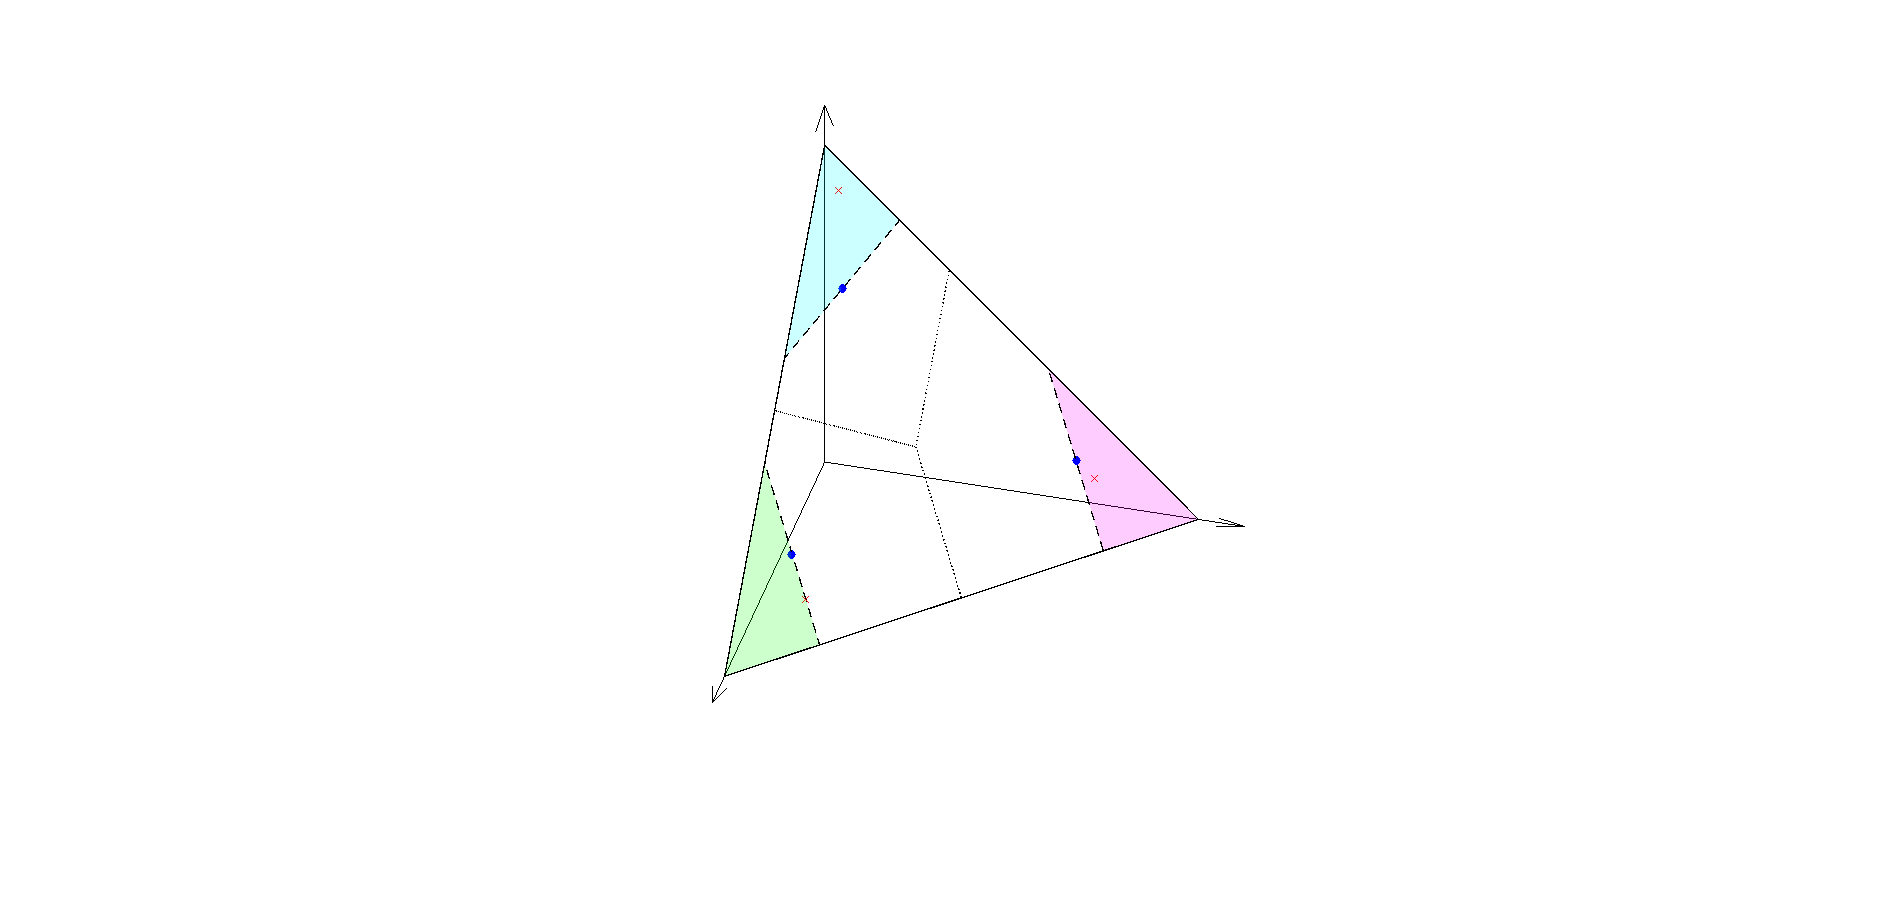
\includegraphics[width=1\linewidth]{figs/partition_symm_with_query.png}
    \caption{State space partitioning of the runtime information vector $\overline{p}$ for $\epsilon = 3.2$. For runtime information vector belong to the darker shaded regions, we obtain $\epsilon$-optimality by reusing a specific strategy $\rho_{\out_{(\cdot)}}$, and avoid computationally expensive re-synthesis.}
    \label{fig:partition}
\end{figure}

 
% Each strategy corresponds to a different ordering of the rooms searched by the robot. We note that all strategies are guaranteed to be correct in that the human will be found. However, the order in which the rooms are visited will affect the expected time to find the human. 

% In the experiment, we start with a $p = [\frac{1}{3},\frac{1}{3},\frac{1}{3}]$. In this case, all the policies are equal, and the robot implements policy 1 shown in Figure~\ref{fig:gazebopolicies1}. Every time the robot `sees' the human in a room, it uses a Bayes update to change its current estimate of $p$. After a certain number of observations, policy 2 was determined to be the most optimal and the robot switches. This is shown in $Figure~\ref{fig:gazebopolicies1}$ which corresponds to visiting the room the human is currently in first. If the human moves to a different room, the robot will eventually switch policies again once the parameter has been updated to reflect the current belief in the human's position. 

We used three candidate instantiations of $\overline{p}$ (Figure~\ref{fig:partition}). The robot only has enough charge to visit one of the three rooms and return to the charging station. The optimal robot strategy for each $\overline p_i$ corresponds to an \emph{ordering} of which room to visit. Intuitively, the robot will visit rooms in decreasing order of likelihood of a human being there, by executing the continuous trajectories shown in Figure~\ref{fig:trivialtrajs}. 


Figure~\ref{fig:partition} shows the partition of the space of $\mathcal{P}$ generated from the corresponding polytopes $\mathcal{S}_i$ for $\epsilon = 3.2$. The choice of $\epsilon$ is dictated by Proposition~\ref{prop:nonempty}. The three candidate instantiations of $\overline{p}$ are represented by colored dots. The darker coloured regions are the polytopes $\mathcal{S}_i$, and they correspond to the regions of $\mathcal{P}$ in which the corresponding strategy is $\epsilon$-optimal. Note that $\mathcal{P}\not\subseteq\cup_{i=1}^N\mathcal{S}_i$, and there are parameters in $\mathcal{P}$ were none of the three strategies are $\epsilon$-optimal. The light shaded areas around each $\overline{p}_i$ corresponds to the portion of the parameter space in which the correspondingly coloured strategy dominates the others, but is not $\epsilon$-optimal.


Table~\ref{tab:perf} shows the proposed optimality bounds obtained from our approach (Theorem~\ref{thm:bounds}). On comparing with the lowest delay possible (computed via re-synthesis), we see that the computed bounds holds in the first two rows.   
 We compute the resulting cost from implementing the corresponding candidate strategy on the simulated turtlebot for different values of $\overline{p}$. We also compute the values of the upper and lower bounds from applying Theorem 1 as well as the true optimal value of the cost. Note that in the first two rows, implementing the pre-computed strategy keeps us within the $\epsilon$-bounds. However, this is not the case for the last row, shaded in red. In this case, $\overline{p} = \lbrack 0.6,0.3,0.1 \rbrack$ lying outside $\cup_{i=1}^N\mathcal{S}_i$ (outside of the dark shaded region in Figure~\ref{fig:partition}), has no informative bounds. Here, $\rho_{\out_1}$ is the dominating strategy among $\rho_{\out_{(\cdot)}}$, with $C(\rho_{\out_1},\overline{p})=13.6$.

A video of the simulation of the robot meeting the human (infinitely often) as the human moves in real-time can be found at \url{https://youtu.be/pn6afwf5INc}.

\subsection{Urban air mobility traffic management}

We now consider an automated air traffic management system for urban air mobility (UAM) operations. The controller is required to optimize the throughput of a multi-pad UAM port, along with bounding the delays experienced by vehicles and passengers. We synthesize a controller for a UAM hub, which consists of a grouping of multiple UAM vertiports. The hub has restrictions on the number of aircraft it is allowed to simultaneously land across all vertiports. Hence, a controller, if necessary, must make incoming air vehicles wait until it is able to safely allow them to land. In this example, we consider three vertiports --- A ($red$), B ($yellow$), and C ($blue$) where an aircraft can request to land. Formally, the task specification is
\vspace{-0.12cm}
\begin{multline*}
    \varphi = \LTLglobally (\text{Current Requests} < R) 
\rightarrow \\ \qquad\;\LTLglobally (\text{No. Landing Aircraft} < M) \; \wedge \\ \LTLglobally (\text{Land Request} \rightarrow \LTLfinally \text{Land Allowed}),
\end{multline*}
where $R$ is maximum number of simultaneous requests and $M$ is the maximum number of aircraft allowed to land simultaneously. We model incoming aircraft as landing requests for vertiports drawn from a time-varying probability distribution. We model the performance metric as the \emph{maximum delay}. The cost function is
\begin{align}
C(\rho_A,\overline{p}) = \max_i(\text{delay}(V_i,\rho_\out))\cdot q_i\label{eq:cost_UAM}
\end{align}
where $\overline{p} = \lbrack q_1 , q_2,q_3,q_4 \rbrack$, $q_i$ is the probability of a request to land at vertiport hub $V_i$ for $i=\{1,2,3\}$, and $q_4$ is the probability of no landing request, and $\text{delay}(V_i,\rho_\out)$ is the processing delay at $V_i$ under strategy $\rho_\out$. We pre-compute strategies for three representative instantiations of the runtime information with each strategy taking 213 s to compute.
Initially, we choose the true distribution to be one of the instantiations. At $t=150$ minutes, the underlying probability distribution of landing requests changes such that the uninformed strategy performs poorly and the new probability value is not part of any of the representative instantiations. At $t=400$ minutes, the probability distribution switches back to the initial probability distribution. The uninformed strategy is a fixed, runtime information-independent strategy that satisfies $\spec$.
 Intuitively, if the hub knew which vertiports were more likely to get landing requests, it would prioritize those vertiports more in order to avoid a backlog of air vehicles waiting to land. The bottom plot in Figure~\ref{fig:delay} shows the probability distribution of requests to each vertiport over time. Green corresponds to no landing request being generated. 
% \begin{figure}
%     \centering
%     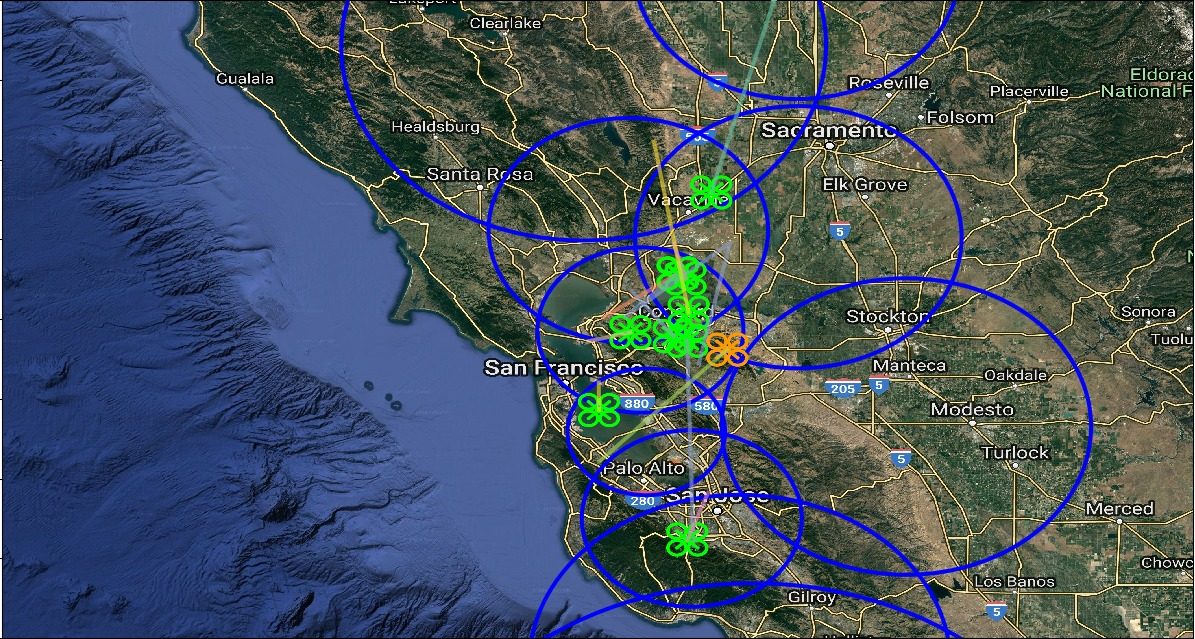
\includegraphics[width=0.85\linewidth]{figs/UAMexample.jpeg}
%     \caption{Place holder for UAM example figure}
%     \label{fig:UAMexample}
% \end{figure}

% Figure~\ref{fig:UAMexample} illustrates the case study. Each blue circle corresponds to the region of influence of a traffic controller. Incoming aircraft request a specific vertiport to land. The controller decides when an aircraft can land. Part of the controller's safety objective is to not allow more than a certain number of aircraft landing simultaneously. 
%
 The information vector in this example conveys the probability distribution over which vertiport incoming aircraft will request. Intuitively, if this information is known beforehand, the controller can prioritize landing requests accordingly to minimize backlog of requests for busy vertiports. 



\begin{figure}
    \centering
    % This file was created by tikzplotlib v0.8.2.
\usepgfplotslibrary{groupplots}

\begin{tikzpicture}
\definecolor{color0}{rgb}{0.12156862745098,0.466666666666667,0.705882352941177}
\definecolor{color1}{rgb}{1,0.498039215686275,0.0549019607843137}
\definecolor{color2}{rgb}{1,1,0}

\begin{groupplot}[group style={group size=1 by 2}]
\nextgroupplot[
legend cell align={left},
height = 5.5cm,
width = 1\linewidth,
legend style={at={(0.36,0.42)}, anchor=north west, draw=white!0.0!black},
tick align=outside,
tick pos=left,
x grid style={white!69.01960784313725!black},
xmin=-27.0875, xmax=552.3375,
xtick style={color=black},
y grid style={white!69.01960784313725!black},
ylabel style = {align=center},
ylabel={Average maximum \\ delay time (min) },
ymin=6.14855, ymax=21.86645,
ytick style={color=black}
]
\path [fill=color0]
(axis cs:159,12.287)
--(axis cs:160,12.428)
--(axis cs:161,12.544)
--(axis cs:162,12.659)
--(axis cs:163,12.785)
--(axis cs:164,12.928)
--(axis cs:165,13.034)
--(axis cs:166,13.146)
--(axis cs:167,13.304)
--(axis cs:168,13.439)
--(axis cs:169,13.587)
--(axis cs:170,13.753)
--(axis cs:171,13.908)
--(axis cs:172,14.079)
--(axis cs:173,14.26)
--(axis cs:174,14.462)
--(axis cs:175,14.654)
--(axis cs:176,14.83)
--(axis cs:177,15.044)
--(axis cs:178,15.239)
--(axis cs:179,15.447)
--(axis cs:180,15.693)
--(axis cs:181,15.946)
--(axis cs:182,16.195)
--(axis cs:183,16.437)
--(axis cs:184,16.604)
--(axis cs:185,16.795)
--(axis cs:186,16.988)
--(axis cs:187,17.157)
--(axis cs:188,17.292)
--(axis cs:189,17.413)
--(axis cs:190,17.548)
--(axis cs:191,17.669)
--(axis cs:192,17.775)
--(axis cs:193,17.881)
--(axis cs:194,17.955)
--(axis cs:195,18.006)
--(axis cs:196,18.064)
--(axis cs:197,18.103)
--(axis cs:198,18.149)
--(axis cs:199,18.185)
--(axis cs:200,18.169)
--(axis cs:201,18.148)
--(axis cs:202,18.123)
--(axis cs:203,18.104)
--(axis cs:204,18.172)
--(axis cs:205,18.186)
--(axis cs:206,18.185)
--(axis cs:207,18.147)
--(axis cs:208,18.145)
--(axis cs:209,18.096)
--(axis cs:210,18.047)
--(axis cs:211,18.042)
--(axis cs:212,18.033)
--(axis cs:213,17.993)
--(axis cs:214,18.001)
--(axis cs:215,18.011)
--(axis cs:216,17.987)
--(axis cs:217,17.925)
--(axis cs:218,17.867)
--(axis cs:219,17.814)
--(axis cs:220,17.756)
--(axis cs:221,17.741)
--(axis cs:222,17.728)
--(axis cs:223,17.721)
--(axis cs:224,17.706)
--(axis cs:225,17.718)
--(axis cs:226,17.713)
--(axis cs:227,17.739)
--(axis cs:228,17.731)
--(axis cs:229,17.746)
--(axis cs:230,17.779)
--(axis cs:231,17.784)
--(axis cs:232,17.805)
--(axis cs:233,17.851)
--(axis cs:234,17.86)
--(axis cs:235,17.901)
--(axis cs:236,17.96)
--(axis cs:237,18.017)
--(axis cs:238,18.094)
--(axis cs:239,18.147)
--(axis cs:240,18.238)
--(axis cs:241,18.272)
--(axis cs:242,18.318)
--(axis cs:243,18.315)
--(axis cs:244,18.254)
--(axis cs:245,18.196)
--(axis cs:246,18.168)
--(axis cs:247,18.171)
--(axis cs:248,18.209)
--(axis cs:249,18.267)
--(axis cs:250,18.281)
--(axis cs:251,18.287)
--(axis cs:252,18.26)
--(axis cs:253,18.252)
--(axis cs:254,18.239)
--(axis cs:255,18.172)
--(axis cs:256,18.09)
--(axis cs:257,18.077)
--(axis cs:258,18.067)
--(axis cs:259,18.077)
--(axis cs:260,18.112)
--(axis cs:261,18.152)
--(axis cs:262,18.163)
--(axis cs:263,18.186)
--(axis cs:264,18.229)
--(axis cs:265,18.288)
--(axis cs:266,18.341)
--(axis cs:267,18.363)
--(axis cs:268,18.394)
--(axis cs:269,18.405)
--(axis cs:270,18.413)
--(axis cs:271,18.424)
--(axis cs:272,18.464)
--(axis cs:273,18.494)
--(axis cs:274,18.498)
--(axis cs:275,18.546)
--(axis cs:276,18.608)
--(axis cs:277,18.645)
--(axis cs:278,18.632)
--(axis cs:279,18.628)
--(axis cs:280,18.586)
--(axis cs:281,18.556)
--(axis cs:282,18.566)
--(axis cs:283,18.615)
--(axis cs:284,18.669)
--(axis cs:285,18.665)
--(axis cs:286,18.617)
--(axis cs:287,18.566)
--(axis cs:288,18.507)
--(axis cs:289,18.447)
--(axis cs:290,18.424)
--(axis cs:291,18.423)
--(axis cs:292,18.397)
--(axis cs:293,18.362)
--(axis cs:294,18.348)
--(axis cs:295,18.33)
--(axis cs:296,18.336)
--(axis cs:297,18.336)
--(axis cs:298,18.343)
--(axis cs:299,18.315)
--(axis cs:300,18.302)
--(axis cs:301,18.29)
--(axis cs:302,18.278)
--(axis cs:303,18.228)
--(axis cs:304,18.182)
--(axis cs:305,18.188)
--(axis cs:306,18.234)
--(axis cs:307,18.289)
--(axis cs:308,18.339)
--(axis cs:309,18.401)
--(axis cs:310,18.442)
--(axis cs:311,18.458)
--(axis cs:312,18.518)
--(axis cs:313,18.581)
--(axis cs:314,18.628)
--(axis cs:315,18.691)
--(axis cs:316,18.743)
--(axis cs:317,18.801)
--(axis cs:318,18.883)
--(axis cs:319,18.972)
--(axis cs:320,19.041)
--(axis cs:321,19.147)
--(axis cs:322,19.232)
--(axis cs:323,19.317)
--(axis cs:324,19.405)
--(axis cs:325,19.504)
--(axis cs:326,19.581)
--(axis cs:327,19.653)
--(axis cs:328,19.711)
--(axis cs:329,19.779)
--(axis cs:330,19.832)
--(axis cs:331,19.896)
--(axis cs:332,19.933)
--(axis cs:333,19.979)
--(axis cs:334,20.055)
--(axis cs:335,20.127)
--(axis cs:336,20.197)
--(axis cs:337,20.242)
--(axis cs:338,20.282)
--(axis cs:339,20.346)
--(axis cs:340,20.414)
--(axis cs:341,20.476)
--(axis cs:342,20.522)
--(axis cs:343,20.578)
--(axis cs:344,20.646)
--(axis cs:345,20.692)
--(axis cs:346,20.697)
--(axis cs:347,20.711)
--(axis cs:348,20.763)
--(axis cs:349,20.792)
--(axis cs:350,20.839)
--(axis cs:351,20.85)
--(axis cs:352,20.859)
--(axis cs:353,20.829)
--(axis cs:354,20.842)
--(axis cs:355,20.862)
--(axis cs:356,20.899)
--(axis cs:357,20.917)
--(axis cs:358,20.93)
--(axis cs:359,20.925)
--(axis cs:360,20.939)
--(axis cs:361,20.933)
--(axis cs:362,20.923)
--(axis cs:363,20.888)
--(axis cs:364,20.848)
--(axis cs:365,20.811)
--(axis cs:366,20.834)
--(axis cs:367,20.86)
--(axis cs:368,20.862)
--(axis cs:369,20.858)
--(axis cs:370,20.827)
--(axis cs:371,20.823)
--(axis cs:372,20.838)
--(axis cs:373,20.888)
--(axis cs:374,20.885)
--(axis cs:375,20.857)
--(axis cs:376,20.791)
--(axis cs:377,20.76)
--(axis cs:378,20.725)
--(axis cs:379,20.701)
--(axis cs:380,20.693)
--(axis cs:381,20.686)
--(axis cs:382,20.687)
--(axis cs:383,20.692)
--(axis cs:384,20.705)
--(axis cs:385,20.684)
--(axis cs:386,20.681)
--(axis cs:387,20.679)
--(axis cs:388,20.673)
--(axis cs:389,20.709)
--(axis cs:390,20.782)
--(axis cs:391,20.815)
--(axis cs:392,20.859)
--(axis cs:393,20.888)
--(axis cs:394,20.913)
--(axis cs:395,20.927)
--(axis cs:396,20.967)
--(axis cs:397,21.023)
--(axis cs:398,21.081)
--(axis cs:399,21.128)
--(axis cs:400,21.131)
--(axis cs:401,21.127)
--(axis cs:402,21.124)
--(axis cs:403,21.13)
--(axis cs:404,21.126)
--(axis cs:405,21.152)
--(axis cs:406,21.12)
--(axis cs:407,21.078)
--(axis cs:408,21.062)
--(axis cs:409,21.023)
--(axis cs:410,20.964)
--(axis cs:411,20.959)
--(axis cs:412,20.937)
--(axis cs:413,20.924)
--(axis cs:414,20.888)
--(axis cs:415,20.83)
--(axis cs:416,20.76)
--(axis cs:417,20.648)
--(axis cs:418,20.538)
--(axis cs:419,20.418)
--(axis cs:420,20.293)
--(axis cs:421,20.166)
--(axis cs:422,20.046)
--(axis cs:423,19.935)
--(axis cs:424,19.769)
--(axis cs:425,19.581)
--(axis cs:426,19.416)
--(axis cs:427,19.246)
--(axis cs:428,19.065)
--(axis cs:429,18.865)
--(axis cs:430,18.658)
--(axis cs:431,18.421)
--(axis cs:432,18.186)
--(axis cs:433,17.953)
--(axis cs:434,17.755)
--(axis cs:435,17.6)
--(axis cs:436,17.448)
--(axis cs:437,17.342)
--(axis cs:438,17.265)
--(axis cs:439,17.21)
--(axis cs:440,17.183)
--(axis cs:441,17.159)
--(axis cs:442,17.139)
--(axis cs:443,17.147)
--(axis cs:444,17.174)
--(axis cs:445,17.228)
--(axis cs:446,17.284)
--(axis cs:447,17.305)
--(axis cs:448,17.327)
--(axis cs:449,17.369)
--(axis cs:450,17.421)
--(axis cs:451,17.465)
--(axis cs:452,17.516)
--(axis cs:453,17.58)
--(axis cs:454,17.661)
--(axis cs:455,17.692)
--(axis cs:456,17.743)
--(axis cs:457,17.763)
--(axis cs:458,17.709)
--(axis cs:459,17.656)
--(axis cs:460,17.606)
--(axis cs:461,17.596)
--(axis cs:462,17.578)
--(axis cs:463,17.551)
--(axis cs:464,17.513)
--(axis cs:465,17.486)
--(axis cs:466,17.466)
--(axis cs:467,17.489)
--(axis cs:468,17.477)
--(axis cs:469,17.479)
--(axis cs:470,17.449)
--(axis cs:471,17.441)
--(axis cs:472,17.4)
--(axis cs:473,17.358)
--(axis cs:474,17.292)
--(axis cs:475,17.276)
--(axis cs:476,17.238)
--(axis cs:477,17.224)
--(axis cs:478,17.248)
--(axis cs:479,17.29)
--(axis cs:480,17.3)
--(axis cs:481,17.258)
--(axis cs:482,17.221)
--(axis cs:483,17.184)
--(axis cs:484,17.192)
--(axis cs:485,17.174)
--(axis cs:486,17.168)
--(axis cs:487,17.166)
--(axis cs:488,17.211)
--(axis cs:489,17.213)
--(axis cs:490,17.251)
--(axis cs:491,17.284)
--(axis cs:492,17.366)
--(axis cs:493,17.419)
--(axis cs:494,17.418)
--(axis cs:495,17.436)
--(axis cs:496,17.459)
--(axis cs:497,17.477)
--(axis cs:498,17.484)
--(axis cs:499,17.494)
--(axis cs:500,17.465)
--(axis cs:501,17.441)
--(axis cs:502,17.379)
--(axis cs:503,17.273)
--(axis cs:504,17.118)
--(axis cs:505,17.012)
--(axis cs:506,16.876)
--(axis cs:507,16.757)
--(axis cs:508,16.617)
--(axis cs:509,16.503)
--(axis cs:510,16.37)
--(axis cs:511,16.194)
--(axis cs:512,15.97)
--(axis cs:513,15.709)
--(axis cs:514,15.448)
--(axis cs:515,15.165)
--(axis cs:516,14.853)
--(axis cs:517,14.491)
--(axis cs:518,14.139)
--(axis cs:519,13.779)
--(axis cs:520,13.466)
--(axis cs:521,13.147)
--(axis cs:522,12.82)
--(axis cs:523,12.504)
--(axis cs:524,12.27)
--(axis cs:524.509554140127,12.1227388535032)
--(axis cs:524,12.19)
--(axis cs:523,12.395)
--(axis cs:522,12.572)
--(axis cs:521,12.802)
--(axis cs:520,13.014)
--(axis cs:519,13.216)
--(axis cs:518,13.384)
--(axis cs:517,13.611)
--(axis cs:516,13.838)
--(axis cs:515,14.084)
--(axis cs:514,14.249)
--(axis cs:513,14.461)
--(axis cs:512,14.627)
--(axis cs:511,14.76)
--(axis cs:510,14.922)
--(axis cs:509,15.053)
--(axis cs:508,15.175)
--(axis cs:507,15.276)
--(axis cs:506,15.394)
--(axis cs:505,15.486)
--(axis cs:504,15.553)
--(axis cs:503,15.571)
--(axis cs:502,15.638)
--(axis cs:501,15.658)
--(axis cs:500,15.699)
--(axis cs:499,15.708)
--(axis cs:498,15.776)
--(axis cs:497,15.819)
--(axis cs:496,15.84)
--(axis cs:495,15.872)
--(axis cs:494,15.923)
--(axis cs:493,15.944)
--(axis cs:492,15.968)
--(axis cs:491,16.005)
--(axis cs:490,16.014)
--(axis cs:489,15.987)
--(axis cs:488,15.963)
--(axis cs:487,15.929)
--(axis cs:486,15.913)
--(axis cs:485,15.952)
--(axis cs:484,16.001)
--(axis cs:483,16.06)
--(axis cs:482,16.084)
--(axis cs:481,16.143)
--(axis cs:480,16.182)
--(axis cs:479,16.211)
--(axis cs:478,16.166)
--(axis cs:477,16.142)
--(axis cs:476,16.131)
--(axis cs:475,16.121)
--(axis cs:474,16.131)
--(axis cs:473,16.126)
--(axis cs:472,16.093)
--(axis cs:471,16.07)
--(axis cs:470,16.079)
--(axis cs:469,16.114)
--(axis cs:468,16.125)
--(axis cs:467,16.159)
--(axis cs:466,16.157)
--(axis cs:465,16.131)
--(axis cs:464,16.068)
--(axis cs:463,16.006)
--(axis cs:462,15.969)
--(axis cs:461,15.944)
--(axis cs:460,15.935)
--(axis cs:459,15.95)
--(axis cs:458,15.972)
--(axis cs:457,15.944)
--(axis cs:456,15.925)
--(axis cs:455,15.939)
--(axis cs:454,15.979)
--(axis cs:453,16.011)
--(axis cs:452,16.07)
--(axis cs:451,16.114)
--(axis cs:450,16.12)
--(axis cs:449,16.072)
--(axis cs:448,16.056)
--(axis cs:447,16.036)
--(axis cs:446,16.041)
--(axis cs:445,16.086)
--(axis cs:444,16.171)
--(axis cs:443,16.283)
--(axis cs:442,16.385)
--(axis cs:441,16.465)
--(axis cs:440,16.54)
--(axis cs:439,16.623)
--(axis cs:438,16.705)
--(axis cs:437,16.811)
--(axis cs:436,16.904)
--(axis cs:435,16.984)
--(axis cs:434,17.047)
--(axis cs:433,17.137)
--(axis cs:432,17.254)
--(axis cs:431,17.392)
--(axis cs:430,17.547)
--(axis cs:429,17.729)
--(axis cs:428,17.946)
--(axis cs:427,18.149)
--(axis cs:426,18.342)
--(axis cs:425,18.459)
--(axis cs:424,18.583)
--(axis cs:423,18.685)
--(axis cs:422,18.792)
--(axis cs:421,18.898)
--(axis cs:420,19.028)
--(axis cs:419,19.153)
--(axis cs:418,19.286)
--(axis cs:417,19.371)
--(axis cs:416,19.472)
--(axis cs:415,19.549)
--(axis cs:414,19.605)
--(axis cs:413,19.652)
--(axis cs:412,19.691)
--(axis cs:411,19.72)
--(axis cs:410,19.736)
--(axis cs:409,19.747)
--(axis cs:408,19.751)
--(axis cs:407,19.771)
--(axis cs:406,19.803)
--(axis cs:405,19.863)
--(axis cs:404,19.873)
--(axis cs:403,19.88)
--(axis cs:402,19.883)
--(axis cs:401,19.92)
--(axis cs:400,19.91)
--(axis cs:399,19.922)
--(axis cs:398,19.905)
--(axis cs:397,19.936)
--(axis cs:396,19.938)
--(axis cs:395,19.966)
--(axis cs:394,20.013)
--(axis cs:393,20.048)
--(axis cs:392,20.073)
--(axis cs:391,20.081)
--(axis cs:390,20.065)
--(axis cs:389,20.059)
--(axis cs:388,20.045)
--(axis cs:387,20.014)
--(axis cs:386,19.995)
--(axis cs:385,19.964)
--(axis cs:384,19.977)
--(axis cs:383,19.969)
--(axis cs:382,19.988)
--(axis cs:381,19.993)
--(axis cs:380,20.034)
--(axis cs:379,20.056)
--(axis cs:378,20.082)
--(axis cs:377,20.118)
--(axis cs:376,20.171)
--(axis cs:375,20.186)
--(axis cs:374,20.153)
--(axis cs:373,20.102)
--(axis cs:372,20.051)
--(axis cs:371,20.015)
--(axis cs:370,19.999)
--(axis cs:369,20.014)
--(axis cs:368,19.989)
--(axis cs:367,19.968)
--(axis cs:366,19.921)
--(axis cs:365,19.904)
--(axis cs:364,19.845)
--(axis cs:363,19.797)
--(axis cs:362,19.736)
--(axis cs:361,19.676)
--(axis cs:360,19.601)
--(axis cs:359,19.536)
--(axis cs:358,19.507)
--(axis cs:357,19.49)
--(axis cs:356,19.481)
--(axis cs:355,19.483)
--(axis cs:354,19.499)
--(axis cs:353,19.553)
--(axis cs:352,19.585)
--(axis cs:351,19.608)
--(axis cs:350,19.631)
--(axis cs:349,19.633)
--(axis cs:348,19.667)
--(axis cs:347,19.702)
--(axis cs:346,19.767)
--(axis cs:345,19.782)
--(axis cs:344,19.828)
--(axis cs:343,19.899)
--(axis cs:342,19.933)
--(axis cs:341,19.926)
--(axis cs:340,19.919)
--(axis cs:339,19.903)
--(axis cs:338,19.909)
--(axis cs:337,19.866)
--(axis cs:336,19.811)
--(axis cs:335,19.74)
--(axis cs:334,19.653)
--(axis cs:333,19.562)
--(axis cs:332,19.462)
--(axis cs:331,19.406)
--(axis cs:330,19.331)
--(axis cs:329,19.245)
--(axis cs:328,19.135)
--(axis cs:327,19.042)
--(axis cs:326,18.928)
--(axis cs:325,18.882)
--(axis cs:324,18.82)
--(axis cs:323,18.694)
--(axis cs:322,18.584)
--(axis cs:321,18.493)
--(axis cs:320,18.408)
--(axis cs:319,18.326)
--(axis cs:318,18.197)
--(axis cs:317,18.046)
--(axis cs:316,17.935)
--(axis cs:315,17.848)
--(axis cs:314,17.796)
--(axis cs:313,17.734)
--(axis cs:312,17.718)
--(axis cs:311,17.666)
--(axis cs:310,17.645)
--(axis cs:309,17.61)
--(axis cs:308,17.582)
--(axis cs:307,17.528)
--(axis cs:306,17.5)
--(axis cs:305,17.459)
--(axis cs:304,17.438)
--(axis cs:303,17.447)
--(axis cs:302,17.476)
--(axis cs:301,17.51)
--(axis cs:300,17.514)
--(axis cs:299,17.499)
--(axis cs:298,17.518)
--(axis cs:297,17.572)
--(axis cs:296,17.582)
--(axis cs:295,17.572)
--(axis cs:294,17.551)
--(axis cs:293,17.54)
--(axis cs:292,17.496)
--(axis cs:291,17.442)
--(axis cs:290,17.371)
--(axis cs:289,17.34)
--(axis cs:288,17.307)
--(axis cs:287,17.286)
--(axis cs:286,17.194)
--(axis cs:285,17.095)
--(axis cs:284,16.986)
--(axis cs:283,16.862)
--(axis cs:282,16.774)
--(axis cs:281,16.638)
--(axis cs:280,16.522)
--(axis cs:279,16.451)
--(axis cs:278,16.348)
--(axis cs:277,16.255)
--(axis cs:276,16.218)
--(axis cs:275,16.195)
--(axis cs:274,16.166)
--(axis cs:273,16.173)
--(axis cs:272,16.169)
--(axis cs:271,16.178)
--(axis cs:270,16.226)
--(axis cs:269,16.233)
--(axis cs:268,16.251)
--(axis cs:267,16.254)
--(axis cs:266,16.295)
--(axis cs:265,16.33)
--(axis cs:264,16.367)
--(axis cs:263,16.424)
--(axis cs:262,16.411)
--(axis cs:261,16.476)
--(axis cs:260,16.534)
--(axis cs:259,16.548)
--(axis cs:258,16.577)
--(axis cs:257,16.611)
--(axis cs:256,16.599)
--(axis cs:255,16.604)
--(axis cs:254,16.649)
--(axis cs:253,16.636)
--(axis cs:252,16.646)
--(axis cs:251,16.712)
--(axis cs:250,16.745)
--(axis cs:249,16.778)
--(axis cs:248,16.789)
--(axis cs:247,16.85)
--(axis cs:246,16.901)
--(axis cs:245,16.944)
--(axis cs:244,16.994)
--(axis cs:243,17.075)
--(axis cs:242,17.151)
--(axis cs:241,17.182)
--(axis cs:240,17.179)
--(axis cs:239,17.2)
--(axis cs:238,17.241)
--(axis cs:237,17.271)
--(axis cs:236,17.301)
--(axis cs:235,17.274)
--(axis cs:234,17.217)
--(axis cs:233,17.187)
--(axis cs:232,17.185)
--(axis cs:231,17.158)
--(axis cs:230,17.104)
--(axis cs:229,17.06)
--(axis cs:228,17.055)
--(axis cs:227,17.038)
--(axis cs:226,17.012)
--(axis cs:225,16.987)
--(axis cs:224,16.944)
--(axis cs:223,16.916)
--(axis cs:222,16.913)
--(axis cs:221,16.899)
--(axis cs:220,16.926)
--(axis cs:219,16.972)
--(axis cs:218,16.978)
--(axis cs:217,16.974)
--(axis cs:216,16.971)
--(axis cs:215,16.99)
--(axis cs:214,16.988)
--(axis cs:213,16.992)
--(axis cs:212,16.979)
--(axis cs:211,16.912)
--(axis cs:210,16.875)
--(axis cs:209,16.843)
--(axis cs:208,16.818)
--(axis cs:207,16.779)
--(axis cs:206,16.759)
--(axis cs:205,16.756)
--(axis cs:204,16.741)
--(axis cs:203,16.736)
--(axis cs:202,16.769)
--(axis cs:201,16.825)
--(axis cs:200,16.871)
--(axis cs:199,16.884)
--(axis cs:198,16.882)
--(axis cs:197,16.873)
--(axis cs:196,16.827)
--(axis cs:195,16.785)
--(axis cs:194,16.767)
--(axis cs:193,16.71)
--(axis cs:192,16.615)
--(axis cs:191,16.542)
--(axis cs:190,16.432)
--(axis cs:189,16.33)
--(axis cs:188,16.168)
--(axis cs:187,15.995)
--(axis cs:186,15.796)
--(axis cs:185,15.555)
--(axis cs:184,15.309)
--(axis cs:183,15.004)
--(axis cs:182,14.669)
--(axis cs:181,14.31)
--(axis cs:180,13.975)
--(axis cs:179,13.629)
--(axis cs:178,13.329)
--(axis cs:177,13.083)
--(axis cs:176,12.871)
--(axis cs:175,12.662)
--(axis cs:174,12.458)
--(axis cs:173,12.281)
--(axis cs:172,12.144)
--(axis cs:171,11.994)
--(axis cs:170,11.852)
--(axis cs:169,11.708)
--(axis cs:168,11.609)
--(axis cs:167,11.495)
--(axis cs:166,11.397)
--(axis cs:165,11.358)
--(axis cs:164,11.35)
--(axis cs:163,11.323)
--(axis cs:162,11.295)
--(axis cs:161,11.274)
--(axis cs:160,11.244)
--cycle;

\path [fill=color1]
(axis cs:159,12.287)
--(axis cs:160,11.244)
--(axis cs:161,11.274)
--(axis cs:162,11.295)
--(axis cs:163,11.323)
--(axis cs:164,11.35)
--(axis cs:165,11.358)
--(axis cs:166,11.397)
--(axis cs:167,11.495)
--(axis cs:168,11.609)
--(axis cs:169,11.708)
--(axis cs:170,11.852)
--(axis cs:171,11.994)
--(axis cs:172,12.144)
--(axis cs:173,12.281)
--(axis cs:173.764705882353,12.4163529411765)
--(axis cs:173,12.255)
--(axis cs:172,12.062)
--(axis cs:171,11.868)
--(axis cs:170,11.68)
--(axis cs:169,11.524)
--(axis cs:168,11.386)
--(axis cs:167,11.269)
--(axis cs:166,11.135)
--(axis cs:165,11.041)
--(axis cs:164,10.948)
--(axis cs:163,10.87)
--(axis cs:162,10.825)
--(axis cs:161,10.736)
--(axis cs:160,10.649)
--cycle;
\path [fill=color1]
(axis cs:178.728395061728,13.5475185185185)
--(axis cs:179,13.629)
--(axis cs:180,13.975)
--(axis cs:181,14.31)
--(axis cs:182,14.669)
--(axis cs:183,15.004)
--(axis cs:184,15.309)
--(axis cs:185,15.555)
--(axis cs:186,15.796)
--(axis cs:187,15.995)
--(axis cs:188,16.168)
--(axis cs:189,16.33)
--(axis cs:190,16.432)
--(axis cs:191,16.542)
--(axis cs:192,16.615)
--(axis cs:193,16.71)
--(axis cs:194,16.767)
--(axis cs:195,16.785)
--(axis cs:196,16.827)
--(axis cs:197,16.873)
--(axis cs:198,16.882)
--(axis cs:199,16.884)
--(axis cs:200,16.871)
--(axis cs:201,16.825)
--(axis cs:202,16.769)
--(axis cs:203,16.736)
--(axis cs:204,16.741)
--(axis cs:205,16.756)
--(axis cs:206,16.759)
--(axis cs:207,16.779)
--(axis cs:208,16.818)
--(axis cs:209,16.843)
--(axis cs:210,16.875)
--(axis cs:211,16.912)
--(axis cs:212,16.979)
--(axis cs:213,16.992)
--(axis cs:214,16.988)
--(axis cs:215,16.99)
--(axis cs:216,16.971)
--(axis cs:217,16.974)
--(axis cs:218,16.978)
--(axis cs:219,16.972)
--(axis cs:220,16.926)
--(axis cs:221,16.899)
--(axis cs:222,16.913)
--(axis cs:223,16.916)
--(axis cs:224,16.944)
--(axis cs:225,16.987)
--(axis cs:226,17.012)
--(axis cs:227,17.038)
--(axis cs:228,17.055)
--(axis cs:229,17.06)
--(axis cs:230,17.104)
--(axis cs:231,17.158)
--(axis cs:232,17.185)
--(axis cs:233,17.187)
--(axis cs:234,17.217)
--(axis cs:235,17.274)
--(axis cs:236,17.301)
--(axis cs:237,17.271)
--(axis cs:238,17.241)
--(axis cs:239,17.2)
--(axis cs:240,17.179)
--(axis cs:241,17.182)
--(axis cs:242,17.151)
--(axis cs:243,17.075)
--(axis cs:244,16.994)
--(axis cs:245,16.944)
--(axis cs:246,16.901)
--(axis cs:247,16.85)
--(axis cs:248,16.789)
--(axis cs:249,16.778)
--(axis cs:250,16.745)
--(axis cs:251,16.712)
--(axis cs:252,16.646)
--(axis cs:253,16.636)
--(axis cs:254,16.649)
--(axis cs:255,16.604)
--(axis cs:256,16.599)
--(axis cs:257,16.611)
--(axis cs:258,16.577)
--(axis cs:259,16.548)
--(axis cs:260,16.534)
--(axis cs:261,16.476)
--(axis cs:262,16.411)
--(axis cs:263,16.424)
--(axis cs:264,16.367)
--(axis cs:265,16.33)
--(axis cs:266,16.295)
--(axis cs:267,16.254)
--(axis cs:268,16.251)
--(axis cs:269,16.233)
--(axis cs:270,16.226)
--(axis cs:271,16.178)
--(axis cs:272,16.169)
--(axis cs:273,16.173)
--(axis cs:274,16.166)
--(axis cs:275,16.195)
--(axis cs:276,16.218)
--(axis cs:277,16.255)
--(axis cs:278,16.348)
--(axis cs:279,16.451)
--(axis cs:280,16.522)
--(axis cs:281,16.638)
--(axis cs:282,16.774)
--(axis cs:283,16.862)
--(axis cs:284,16.986)
--(axis cs:285,17.095)
--(axis cs:286,17.194)
--(axis cs:287,17.286)
--(axis cs:288,17.307)
--(axis cs:289,17.34)
--(axis cs:290,17.371)
--(axis cs:291,17.442)
--(axis cs:292,17.496)
--(axis cs:293,17.54)
--(axis cs:294,17.551)
--(axis cs:295,17.572)
--(axis cs:296,17.582)
--(axis cs:297,17.572)
--(axis cs:298,17.518)
--(axis cs:299,17.499)
--(axis cs:300,17.514)
--(axis cs:301,17.51)
--(axis cs:302,17.476)
--(axis cs:303,17.447)
--(axis cs:304,17.438)
--(axis cs:305,17.459)
--(axis cs:306,17.5)
--(axis cs:307,17.528)
--(axis cs:308,17.582)
--(axis cs:309,17.61)
--(axis cs:310,17.645)
--(axis cs:311,17.666)
--(axis cs:312,17.718)
--(axis cs:313,17.734)
--(axis cs:314,17.796)
--(axis cs:315,17.848)
--(axis cs:316,17.935)
--(axis cs:317,18.046)
--(axis cs:318,18.197)
--(axis cs:319,18.326)
--(axis cs:320,18.408)
--(axis cs:321,18.493)
--(axis cs:322,18.584)
--(axis cs:323,18.694)
--(axis cs:324,18.82)
--(axis cs:325,18.882)
--(axis cs:326,18.928)
--(axis cs:327,19.042)
--(axis cs:328,19.135)
--(axis cs:329,19.245)
--(axis cs:330,19.331)
--(axis cs:331,19.406)
--(axis cs:332,19.462)
--(axis cs:333,19.562)
--(axis cs:334,19.653)
--(axis cs:335,19.74)
--(axis cs:336,19.811)
--(axis cs:337,19.866)
--(axis cs:338,19.909)
--(axis cs:339,19.903)
--(axis cs:340,19.919)
--(axis cs:341,19.926)
--(axis cs:342,19.933)
--(axis cs:343,19.899)
--(axis cs:344,19.828)
--(axis cs:345,19.782)
--(axis cs:346,19.767)
--(axis cs:347,19.702)
--(axis cs:348,19.667)
--(axis cs:349,19.633)
--(axis cs:350,19.631)
--(axis cs:351,19.608)
--(axis cs:352,19.585)
--(axis cs:353,19.553)
--(axis cs:354,19.499)
--(axis cs:355,19.483)
--(axis cs:356,19.481)
--(axis cs:357,19.49)
--(axis cs:358,19.507)
--(axis cs:359,19.536)
--(axis cs:360,19.601)
--(axis cs:361,19.676)
--(axis cs:362,19.736)
--(axis cs:363,19.797)
--(axis cs:364,19.845)
--(axis cs:365,19.904)
--(axis cs:366,19.921)
--(axis cs:367,19.968)
--(axis cs:368,19.989)
--(axis cs:369,20.014)
--(axis cs:370,19.999)
--(axis cs:371,20.015)
--(axis cs:372,20.051)
--(axis cs:373,20.102)
--(axis cs:374,20.153)
--(axis cs:375,20.186)
--(axis cs:376,20.171)
--(axis cs:377,20.118)
--(axis cs:378,20.082)
--(axis cs:379,20.056)
--(axis cs:380,20.034)
--(axis cs:381,19.993)
--(axis cs:382,19.988)
--(axis cs:383,19.969)
--(axis cs:384,19.977)
--(axis cs:385,19.964)
--(axis cs:386,19.995)
--(axis cs:387,20.014)
--(axis cs:388,20.045)
--(axis cs:389,20.059)
--(axis cs:390,20.065)
--(axis cs:391,20.081)
--(axis cs:392,20.073)
--(axis cs:393,20.048)
--(axis cs:394,20.013)
--(axis cs:395,19.966)
--(axis cs:396,19.938)
--(axis cs:397,19.936)
--(axis cs:398,19.905)
--(axis cs:399,19.922)
--(axis cs:400,19.91)
--(axis cs:401,19.92)
--(axis cs:402,19.883)
--(axis cs:403,19.88)
--(axis cs:404,19.873)
--(axis cs:405,19.863)
--(axis cs:406,19.803)
--(axis cs:407,19.771)
--(axis cs:408,19.751)
--(axis cs:409,19.747)
--(axis cs:410,19.736)
--(axis cs:411,19.72)
--(axis cs:412,19.691)
--(axis cs:413,19.652)
--(axis cs:414,19.605)
--(axis cs:415,19.549)
--(axis cs:416,19.472)
--(axis cs:417,19.371)
--(axis cs:418,19.286)
--(axis cs:419,19.153)
--(axis cs:420,19.028)
--(axis cs:421,18.898)
--(axis cs:422,18.792)
--(axis cs:423,18.685)
--(axis cs:424,18.583)
--(axis cs:425,18.459)
--(axis cs:426,18.342)
--(axis cs:427,18.149)
--(axis cs:428,17.946)
--(axis cs:429,17.729)
--(axis cs:430,17.547)
--(axis cs:431,17.392)
--(axis cs:432,17.254)
--(axis cs:433,17.137)
--(axis cs:434,17.047)
--(axis cs:435,16.984)
--(axis cs:436,16.904)
--(axis cs:437,16.811)
--(axis cs:438,16.705)
--(axis cs:439,16.623)
--(axis cs:440,16.54)
--(axis cs:441,16.465)
--(axis cs:442,16.385)
--(axis cs:443,16.283)
--(axis cs:444,16.171)
--(axis cs:445,16.086)
--(axis cs:446,16.041)
--(axis cs:447,16.036)
--(axis cs:448,16.056)
--(axis cs:449,16.072)
--(axis cs:450,16.12)
--(axis cs:451,16.114)
--(axis cs:452,16.07)
--(axis cs:453,16.011)
--(axis cs:454,15.979)
--(axis cs:455,15.939)
--(axis cs:456,15.925)
--(axis cs:457,15.944)
--(axis cs:458,15.972)
--(axis cs:459,15.95)
--(axis cs:460,15.935)
--(axis cs:461,15.944)
--(axis cs:462,15.969)
--(axis cs:463,16.006)
--(axis cs:464,16.068)
--(axis cs:465,16.131)
--(axis cs:466,16.157)
--(axis cs:467,16.159)
--(axis cs:468,16.125)
--(axis cs:469,16.114)
--(axis cs:470,16.079)
--(axis cs:471,16.07)
--(axis cs:472,16.093)
--(axis cs:473,16.126)
--(axis cs:474,16.131)
--(axis cs:475,16.121)
--(axis cs:476,16.131)
--(axis cs:477,16.142)
--(axis cs:478,16.166)
--(axis cs:479,16.211)
--(axis cs:480,16.182)
--(axis cs:481,16.143)
--(axis cs:482,16.084)
--(axis cs:483,16.06)
--(axis cs:484,16.001)
--(axis cs:485,15.952)
--(axis cs:486,15.913)
--(axis cs:487,15.929)
--(axis cs:488,15.963)
--(axis cs:489,15.987)
--(axis cs:490,16.014)
--(axis cs:491,16.005)
--(axis cs:492,15.968)
--(axis cs:493,15.944)
--(axis cs:494,15.923)
--(axis cs:495,15.872)
--(axis cs:496,15.84)
--(axis cs:497,15.819)
--(axis cs:498,15.776)
--(axis cs:499,15.708)
--(axis cs:500,15.699)
--(axis cs:501,15.658)
--(axis cs:502,15.638)
--(axis cs:503,15.571)
--(axis cs:504,15.553)
--(axis cs:505,15.486)
--(axis cs:506,15.394)
--(axis cs:507,15.276)
--(axis cs:508,15.175)
--(axis cs:509,15.053)
--(axis cs:510,14.922)
--(axis cs:511,14.76)
--(axis cs:512,14.627)
--(axis cs:513,14.461)
--(axis cs:514,14.249)
--(axis cs:515,14.084)
--(axis cs:515.182926829268,14.039)
--(axis cs:515,14.069)
--(axis cs:514,14.223)
--(axis cs:513,14.318)
--(axis cs:512,14.386)
--(axis cs:511,14.461)
--(axis cs:510,14.5)
--(axis cs:509,14.581)
--(axis cs:508,14.674)
--(axis cs:507,14.724)
--(axis cs:506,14.774)
--(axis cs:505,14.881)
--(axis cs:504,14.96)
--(axis cs:503,15.007)
--(axis cs:502,15.034)
--(axis cs:501,15.069)
--(axis cs:500,15.143)
--(axis cs:499,15.22)
--(axis cs:498,15.291)
--(axis cs:497,15.327)
--(axis cs:496,15.383)
--(axis cs:495,15.392)
--(axis cs:494,15.381)
--(axis cs:493,15.372)
--(axis cs:492,15.372)
--(axis cs:491,15.38)
--(axis cs:490,15.428)
--(axis cs:489,15.471)
--(axis cs:488,15.46)
--(axis cs:487,15.485)
--(axis cs:486,15.544)
--(axis cs:485,15.569)
--(axis cs:484,15.611)
--(axis cs:483,15.635)
--(axis cs:482,15.654)
--(axis cs:481,15.667)
--(axis cs:480,15.685)
--(axis cs:479,15.687)
--(axis cs:478,15.705)
--(axis cs:477,15.732)
--(axis cs:476,15.747)
--(axis cs:475,15.764)
--(axis cs:474,15.802)
--(axis cs:473,15.811)
--(axis cs:472,15.813)
--(axis cs:471,15.824)
--(axis cs:470,15.811)
--(axis cs:469,15.807)
--(axis cs:468,15.813)
--(axis cs:467,15.788)
--(axis cs:466,15.768)
--(axis cs:465,15.748)
--(axis cs:464,15.709)
--(axis cs:463,15.71)
--(axis cs:462,15.719)
--(axis cs:461,15.703)
--(axis cs:460,15.695)
--(axis cs:459,15.677)
--(axis cs:458,15.63)
--(axis cs:457,15.633)
--(axis cs:456,15.641)
--(axis cs:455,15.642)
--(axis cs:454,15.617)
--(axis cs:453,15.633)
--(axis cs:452,15.614)
--(axis cs:451,15.577)
--(axis cs:450,15.56)
--(axis cs:449,15.547)
--(axis cs:448,15.569)
--(axis cs:447,15.561)
--(axis cs:446,15.538)
--(axis cs:445,15.531)
--(axis cs:444,15.557)
--(axis cs:443,15.584)
--(axis cs:442,15.62)
--(axis cs:441,15.659)
--(axis cs:440,15.695)
--(axis cs:439,15.761)
--(axis cs:438,15.848)
--(axis cs:437,15.895)
--(axis cs:436,15.96)
--(axis cs:435,16.069)
--(axis cs:434,16.183)
--(axis cs:433,16.26)
--(axis cs:432,16.396)
--(axis cs:431,16.542)
--(axis cs:430,16.694)
--(axis cs:429,16.824)
--(axis cs:428,16.936)
--(axis cs:427,17.08)
--(axis cs:426,17.228)
--(axis cs:425,17.359)
--(axis cs:424,17.477)
--(axis cs:423,17.58)
--(axis cs:422,17.714)
--(axis cs:421,17.816)
--(axis cs:420,17.939)
--(axis cs:419,18.045)
--(axis cs:418,18.166)
--(axis cs:417,18.277)
--(axis cs:416,18.415)
--(axis cs:415,18.5)
--(axis cs:414,18.584)
--(axis cs:413,18.692)
--(axis cs:412,18.76)
--(axis cs:411,18.831)
--(axis cs:410,18.886)
--(axis cs:409,18.959)
--(axis cs:408,19.003)
--(axis cs:407,19.04)
--(axis cs:406,19.072)
--(axis cs:405,19.11)
--(axis cs:404,19.173)
--(axis cs:403,19.228)
--(axis cs:402,19.212)
--(axis cs:401,19.238)
--(axis cs:400,19.233)
--(axis cs:399,19.241)
--(axis cs:398,19.226)
--(axis cs:397,19.248)
--(axis cs:396,19.232)
--(axis cs:395,19.201)
--(axis cs:394,19.139)
--(axis cs:393,19.09)
--(axis cs:392,19.034)
--(axis cs:391,18.973)
--(axis cs:390,18.914)
--(axis cs:389,18.845)
--(axis cs:388,18.808)
--(axis cs:387,18.786)
--(axis cs:386,18.785)
--(axis cs:385,18.787)
--(axis cs:384,18.763)
--(axis cs:383,18.743)
--(axis cs:382,18.767)
--(axis cs:381,18.764)
--(axis cs:380,18.76)
--(axis cs:379,18.752)
--(axis cs:378,18.759)
--(axis cs:377,18.754)
--(axis cs:376,18.751)
--(axis cs:375,18.741)
--(axis cs:374,18.767)
--(axis cs:373,18.8)
--(axis cs:372,18.828)
--(axis cs:371,18.86)
--(axis cs:370,18.866)
--(axis cs:369,18.881)
--(axis cs:368,18.918)
--(axis cs:367,18.923)
--(axis cs:366,18.903)
--(axis cs:365,18.854)
--(axis cs:364,18.834)
--(axis cs:363,18.81)
--(axis cs:362,18.764)
--(axis cs:361,18.712)
--(axis cs:360,18.663)
--(axis cs:359,18.601)
--(axis cs:358,18.544)
--(axis cs:357,18.489)
--(axis cs:356,18.457)
--(axis cs:355,18.438)
--(axis cs:354,18.386)
--(axis cs:353,18.289)
--(axis cs:352,18.228)
--(axis cs:351,18.152)
--(axis cs:350,18.103)
--(axis cs:349,18.062)
--(axis cs:348,17.99)
--(axis cs:347,17.931)
--(axis cs:346,17.883)
--(axis cs:345,17.883)
--(axis cs:344,17.839)
--(axis cs:343,17.819)
--(axis cs:342,17.799)
--(axis cs:341,17.789)
--(axis cs:340,17.786)
--(axis cs:339,17.797)
--(axis cs:338,17.808)
--(axis cs:337,17.776)
--(axis cs:336,17.734)
--(axis cs:335,17.727)
--(axis cs:334,17.738)
--(axis cs:333,17.766)
--(axis cs:332,17.77)
--(axis cs:331,17.761)
--(axis cs:330,17.732)
--(axis cs:329,17.666)
--(axis cs:328,17.634)
--(axis cs:327,17.633)
--(axis cs:326,17.599)
--(axis cs:325,17.538)
--(axis cs:324,17.494)
--(axis cs:323,17.421)
--(axis cs:322,17.342)
--(axis cs:321,17.282)
--(axis cs:320,17.208)
--(axis cs:319,17.141)
--(axis cs:318,17.04)
--(axis cs:317,16.959)
--(axis cs:316,16.849)
--(axis cs:315,16.713)
--(axis cs:314,16.562)
--(axis cs:313,16.447)
--(axis cs:312,16.327)
--(axis cs:311,16.24)
--(axis cs:310,16.156)
--(axis cs:309,16.087)
--(axis cs:308,16)
--(axis cs:307,15.893)
--(axis cs:306,15.829)
--(axis cs:305,15.783)
--(axis cs:304,15.741)
--(axis cs:303,15.689)
--(axis cs:302,15.652)
--(axis cs:301,15.601)
--(axis cs:300,15.565)
--(axis cs:299,15.523)
--(axis cs:298,15.468)
--(axis cs:297,15.407)
--(axis cs:296,15.367)
--(axis cs:295,15.387)
--(axis cs:294,15.416)
--(axis cs:293,15.431)
--(axis cs:292,15.44)
--(axis cs:291,15.453)
--(axis cs:290,15.495)
--(axis cs:289,15.555)
--(axis cs:288,15.627)
--(axis cs:287,15.706)
--(axis cs:286,15.727)
--(axis cs:285,15.707)
--(axis cs:284,15.684)
--(axis cs:283,15.678)
--(axis cs:282,15.67)
--(axis cs:281,15.697)
--(axis cs:280,15.736)
--(axis cs:279,15.767)
--(axis cs:278,15.834)
--(axis cs:277,15.906)
--(axis cs:276,15.979)
--(axis cs:275,16.005)
--(axis cs:274,16.007)
--(axis cs:273,15.965)
--(axis cs:272,15.98)
--(axis cs:271,15.964)
--(axis cs:270,15.936)
--(axis cs:269,15.892)
--(axis cs:268,15.842)
--(axis cs:267,15.799)
--(axis cs:266,15.8)
--(axis cs:265,15.827)
--(axis cs:264,15.834)
--(axis cs:263,15.864)
--(axis cs:262,15.92)
--(axis cs:261,15.96)
--(axis cs:260,15.961)
--(axis cs:259,15.943)
--(axis cs:258,15.896)
--(axis cs:257,15.861)
--(axis cs:256,15.816)
--(axis cs:255,15.785)
--(axis cs:254,15.816)
--(axis cs:253,15.863)
--(axis cs:252,15.881)
--(axis cs:251,15.92)
--(axis cs:250,15.939)
--(axis cs:249,15.949)
--(axis cs:248,15.94)
--(axis cs:247,15.955)
--(axis cs:246,15.978)
--(axis cs:245,16)
--(axis cs:244,16.029)
--(axis cs:243,16.032)
--(axis cs:242,15.995)
--(axis cs:241,15.94)
--(axis cs:240,15.884)
--(axis cs:239,15.883)
--(axis cs:238,15.878)
--(axis cs:237,15.904)
--(axis cs:236,15.914)
--(axis cs:235,15.926)
--(axis cs:234,15.909)
--(axis cs:233,15.892)
--(axis cs:232,15.869)
--(axis cs:231,15.825)
--(axis cs:230,15.797)
--(axis cs:229,15.767)
--(axis cs:228,15.736)
--(axis cs:227,15.67)
--(axis cs:226,15.564)
--(axis cs:225,15.472)
--(axis cs:224,15.417)
--(axis cs:223,15.35)
--(axis cs:222,15.355)
--(axis cs:221,15.371)
--(axis cs:220,15.391)
--(axis cs:219,15.353)
--(axis cs:218,15.353)
--(axis cs:217,15.342)
--(axis cs:216,15.332)
--(axis cs:215,15.281)
--(axis cs:214,15.284)
--(axis cs:213,15.27)
--(axis cs:212,15.272)
--(axis cs:211,15.314)
--(axis cs:210,15.394)
--(axis cs:209,15.462)
--(axis cs:208,15.515)
--(axis cs:207,15.591)
--(axis cs:206,15.688)
--(axis cs:205,15.765)
--(axis cs:204,15.814)
--(axis cs:203,15.878)
--(axis cs:202,15.874)
--(axis cs:201,15.895)
--(axis cs:200,15.912)
--(axis cs:199,15.921)
--(axis cs:198,15.916)
--(axis cs:197,15.903)
--(axis cs:196,15.896)
--(axis cs:195,15.899)
--(axis cs:194,15.857)
--(axis cs:193,15.834)
--(axis cs:192,15.788)
--(axis cs:191,15.701)
--(axis cs:190,15.592)
--(axis cs:189,15.474)
--(axis cs:188,15.358)
--(axis cs:187,15.188)
--(axis cs:186,15.025)
--(axis cs:185,14.833)
--(axis cs:184,14.636)
--(axis cs:183,14.426)
--(axis cs:182,14.213)
--(axis cs:181,13.996)
--(axis cs:180,13.794)
--(axis cs:179,13.607)
--cycle;
\path [fill=color1]
(axis cs:525.596638655462,11.9989327731092)
--(axis cs:526,11.959)
--(axis cs:526,11.959)
--(axis cs:526,11.911)
--cycle;

\addplot [ultra thick, black]
table {%
10 6.863
11 7.324
12 7.754
13 8.163
14 8.5
15 8.814
16 9.088
17 9.31
18 9.504
19 9.67
20 9.791
21 9.869
22 9.868
23 9.832
24 9.8
25 9.756
26 9.751
27 9.794
28 9.864
29 9.927
30 9.951
31 9.975
32 10.007
33 10.045
34 10.083
35 10.121
36 10.146
37 10.188
38 10.229
39 10.268
40 10.308
41 10.343
42 10.403
43 10.461
44 10.511
45 10.585
46 10.647
47 10.644
48 10.644
49 10.662
50 10.669
51 10.674
52 10.638
53 10.6
54 10.611
55 10.546
56 10.496
57 10.442
58 10.405
59 10.366
60 10.372
61 10.373
62 10.39
63 10.459
64 10.503
65 10.551
66 10.559
67 10.547
68 10.529
69 10.514
70 10.557
71 10.556
72 10.584
73 10.579
74 10.562
75 10.597
76 10.632
77 10.681
78 10.694
79 10.684
80 10.641
81 10.601
82 10.556
83 10.503
84 10.471
85 10.437
86 10.448
87 10.515
88 10.554
89 10.59
90 10.602
91 10.636
92 10.66
93 10.656
94 10.655
95 10.65
96 10.647
97 10.638
98 10.642
99 10.629
100 10.618
101 10.645
102 10.621
103 10.589
104 10.558
105 10.527
106 10.521
107 10.529
108 10.505
109 10.461
110 10.413
111 10.376
112 10.319
113 10.322
114 10.331
115 10.359
116 10.376
117 10.402
118 10.406
119 10.445
120 10.479
121 10.487
122 10.506
123 10.53
124 10.514
125 10.454
126 10.38
127 10.273
128 10.276
129 10.276
130 10.279
131 10.268
132 10.271
133 10.238
134 10.191
135 10.121
136 10.099
137 10.046
138 10.016
139 9.991
140 9.951
141 9.931
142 9.97
143 10.007
144 10.074
145 10.202
146 10.331
147 10.462
148 10.567
149 10.705
150 10.834
151 10.999
152 11.166
153 11.338
154 11.506
155 11.693
156 11.847
157 11.993
158 12.142
159 12.287
160 12.428
161 12.544
162 12.659
163 12.785
164 12.928
165 13.034
166 13.146
167 13.304
168 13.439
169 13.587
170 13.753
171 13.908
172 14.079
173 14.26
174 14.462
175 14.654
176 14.83
177 15.044
178 15.239
179 15.447
180 15.693
181 15.946
182 16.195
183 16.437
184 16.604
185 16.795
186 16.988
187 17.157
188 17.292
189 17.413
190 17.548
191 17.669
192 17.775
193 17.881
194 17.955
195 18.006
196 18.064
197 18.103
198 18.149
199 18.185
200 18.169
201 18.148
202 18.123
203 18.104
204 18.172
205 18.186
206 18.185
207 18.147
208 18.145
209 18.096
210 18.047
211 18.042
212 18.033
213 17.993
214 18.001
215 18.011
216 17.987
217 17.925
218 17.867
219 17.814
220 17.756
221 17.741
222 17.728
223 17.721
224 17.706
225 17.718
226 17.713
227 17.739
228 17.731
229 17.746
230 17.779
231 17.784
232 17.805
233 17.851
234 17.86
235 17.901
236 17.96
237 18.017
238 18.094
239 18.147
240 18.238
241 18.272
242 18.318
243 18.315
244 18.254
245 18.196
246 18.168
247 18.171
248 18.209
249 18.267
250 18.281
251 18.287
252 18.26
253 18.252
254 18.239
255 18.172
256 18.09
257 18.077
258 18.067
259 18.077
260 18.112
261 18.152
262 18.163
263 18.186
264 18.229
265 18.288
266 18.341
267 18.363
268 18.394
269 18.405
270 18.413
271 18.424
272 18.464
273 18.494
274 18.498
275 18.546
276 18.608
277 18.645
278 18.632
279 18.628
280 18.586
281 18.556
282 18.566
283 18.615
284 18.669
285 18.665
286 18.617
287 18.566
288 18.507
289 18.447
290 18.424
291 18.423
292 18.397
293 18.362
294 18.348
295 18.33
296 18.336
297 18.336
298 18.343
299 18.315
300 18.302
301 18.29
302 18.278
303 18.228
304 18.182
305 18.188
306 18.234
307 18.289
308 18.339
309 18.401
310 18.442
311 18.458
312 18.518
313 18.581
314 18.628
315 18.691
316 18.743
317 18.801
318 18.883
319 18.972
320 19.041
321 19.147
322 19.232
323 19.317
324 19.405
325 19.504
326 19.581
327 19.653
328 19.711
329 19.779
330 19.832
331 19.896
332 19.933
333 19.979
334 20.055
335 20.127
336 20.197
337 20.242
338 20.282
339 20.346
340 20.414
341 20.476
342 20.522
343 20.578
344 20.646
345 20.692
346 20.697
347 20.711
348 20.763
349 20.792
350 20.839
351 20.85
352 20.859
353 20.829
354 20.842
355 20.862
356 20.899
357 20.917
358 20.93
359 20.925
360 20.939
361 20.933
362 20.923
363 20.888
364 20.848
365 20.811
366 20.834
367 20.86
368 20.862
369 20.858
370 20.827
371 20.823
372 20.838
373 20.888
374 20.885
375 20.857
376 20.791
377 20.76
378 20.725
379 20.701
380 20.693
381 20.686
382 20.687
383 20.692
384 20.705
385 20.684
386 20.681
387 20.679
388 20.673
389 20.709
390 20.782
391 20.815
392 20.859
393 20.888
394 20.913
395 20.927
396 20.967
397 21.023
398 21.081
399 21.128
400 21.131
401 21.127
402 21.124
403 21.13
404 21.126
405 21.152
406 21.12
407 21.078
408 21.062
409 21.023
410 20.964
411 20.959
412 20.937
413 20.924
414 20.888
415 20.83
416 20.76
417 20.648
418 20.538
419 20.418
420 20.293
421 20.166
422 20.046
423 19.935
424 19.769
425 19.581
426 19.416
427 19.246
428 19.065
429 18.865
430 18.658
431 18.421
432 18.186
433 17.953
434 17.755
435 17.6
436 17.448
437 17.342
438 17.265
439 17.21
440 17.183
441 17.159
442 17.139
443 17.147
444 17.174
445 17.228
446 17.284
447 17.305
448 17.327
449 17.369
450 17.421
451 17.465
452 17.516
453 17.58
454 17.661
455 17.692
456 17.743
457 17.763
458 17.709
459 17.656
460 17.606
461 17.596
462 17.578
463 17.551
464 17.513
465 17.486
466 17.466
467 17.489
468 17.477
469 17.479
470 17.449
471 17.441
472 17.4
473 17.358
474 17.292
475 17.276
476 17.238
477 17.224
478 17.248
479 17.29
480 17.3
481 17.258
482 17.221
483 17.184
484 17.192
485 17.174
486 17.168
487 17.166
488 17.211
489 17.213
490 17.251
491 17.284
492 17.366
493 17.419
494 17.418
495 17.436
496 17.459
497 17.477
498 17.484
499 17.494
500 17.465
501 17.441
502 17.379
503 17.273
504 17.118
505 17.012
506 16.876
507 16.757
508 16.617
509 16.503
510 16.37
511 16.194
512 15.97
513 15.709
514 15.448
515 15.165
516 14.853
517 14.491
518 14.139
519 13.779
520 13.466
521 13.147
522 12.82
523 12.504
524 12.27
525 11.981
526 11.713
};
\addlegendentry{Uninformed strategy}
\addplot [ultra thick, green]
table {%
10 6.863
11 7.324
12 7.754
13 8.163
14 8.5
15 8.814
16 9.088
17 9.31
18 9.504
19 9.67
20 9.791
21 9.869
22 9.868
23 9.832
24 9.8
25 9.756
26 9.751
27 9.794
28 9.864
29 9.927
30 9.951
31 9.975
32 10.007
33 10.045
34 10.083
35 10.121
36 10.146
37 10.188
38 10.229
39 10.268
40 10.308
41 10.343
42 10.403
43 10.461
44 10.511
45 10.585
46 10.647
47 10.644
48 10.644
49 10.662
50 10.669
51 10.674
52 10.638
53 10.6
54 10.611
55 10.546
56 10.496
57 10.442
58 10.405
59 10.366
60 10.372
61 10.373
62 10.39
63 10.459
64 10.503
65 10.551
66 10.559
67 10.547
68 10.529
69 10.514
70 10.557
71 10.556
72 10.584
73 10.579
74 10.562
75 10.597
76 10.632
77 10.681
78 10.694
79 10.684
80 10.641
81 10.601
82 10.556
83 10.503
84 10.471
85 10.437
86 10.448
87 10.515
88 10.554
89 10.59
90 10.602
91 10.636
92 10.66
93 10.656
94 10.655
95 10.65
96 10.647
97 10.638
98 10.642
99 10.629
100 10.618
101 10.645
102 10.621
103 10.589
104 10.558
105 10.527
106 10.521
107 10.529
108 10.505
109 10.461
110 10.413
111 10.376
112 10.319
113 10.322
114 10.331
115 10.359
116 10.376
117 10.402
118 10.406
119 10.445
120 10.479
121 10.487
122 10.506
123 10.53
124 10.514
125 10.454
126 10.38
127 10.273
128 10.276
129 10.276
130 10.279
131 10.268
132 10.271
133 10.238
134 10.191
135 10.121
136 10.099
137 10.046
138 10.016
139 9.991
140 9.951
141 9.931
142 9.97
143 10.007
144 10.074
145 10.202
146 10.331
147 10.462
148 10.567
149 10.705
150 10.834
151 10.999
152 11.166
153 11.338
154 11.506
155 11.693
156 11.847
157 11.993
158 12.142
159 12.287
160 10.649
161 10.736
162 10.825
163 10.87
164 10.948
165 11.041
166 11.135
167 11.269
168 11.386
169 11.524
170 11.68
171 11.868
172 12.062
173 12.255
174 12.466
175 12.685
176 12.89
177 13.126
178 13.388
179 13.607
180 13.794
181 13.996
182 14.213
183 14.426
184 14.636
185 14.833
186 15.025
187 15.188
188 15.358
189 15.474
190 15.592
191 15.701
192 15.788
193 15.834
194 15.857
195 15.899
196 15.896
197 15.903
198 15.916
199 15.921
200 15.912
201 15.895
202 15.874
203 15.878
204 15.814
205 15.765
206 15.688
207 15.591
208 15.515
209 15.462
210 15.394
211 15.314
212 15.272
213 15.27
214 15.284
215 15.281
216 15.332
217 15.342
218 15.353
219 15.353
220 15.391
221 15.371
222 15.355
223 15.35
224 15.417
225 15.472
226 15.564
227 15.67
228 15.736
229 15.767
230 15.797
231 15.825
232 15.869
233 15.892
234 15.909
235 15.926
236 15.914
237 15.904
238 15.878
239 15.883
240 15.884
241 15.94
242 15.995
243 16.032
244 16.029
245 16
246 15.978
247 15.955
248 15.94
249 15.949
250 15.939
251 15.92
252 15.881
253 15.863
254 15.816
255 15.785
256 15.816
257 15.861
258 15.896
259 15.943
260 15.961
261 15.96
262 15.92
263 15.864
264 15.834
265 15.827
266 15.8
267 15.799
268 15.842
269 15.892
270 15.936
271 15.964
272 15.98
273 15.965
274 16.007
275 16.005
276 15.979
277 15.906
278 15.834
279 15.767
280 15.736
281 15.697
282 15.67
283 15.678
284 15.684
285 15.707
286 15.727
287 15.706
288 15.627
289 15.555
290 15.495
291 15.453
292 15.44
293 15.431
294 15.416
295 15.387
296 15.367
297 15.407
298 15.468
299 15.523
300 15.565
301 15.601
302 15.652
303 15.689
304 15.741
305 15.783
306 15.829
307 15.893
308 16
309 16.087
310 16.156
311 16.24
312 16.327
313 16.447
314 16.562
315 16.713
316 16.849
317 16.959
318 17.04
319 17.141
320 17.208
321 17.282
322 17.342
323 17.421
324 17.494
325 17.538
326 17.599
327 17.633
328 17.634
329 17.666
330 17.732
331 17.761
332 17.77
333 17.766
334 17.738
335 17.727
336 17.734
337 17.776
338 17.808
339 17.797
340 17.786
341 17.789
342 17.799
343 17.819
344 17.839
345 17.883
346 17.883
347 17.931
348 17.99
349 18.062
350 18.103
351 18.152
352 18.228
353 18.289
354 18.386
355 18.438
356 18.457
357 18.489
358 18.544
359 18.601
360 18.663
361 18.712
362 18.764
363 18.81
364 18.834
365 18.854
366 18.903
367 18.923
368 18.918
369 18.881
370 18.866
371 18.86
372 18.828
373 18.8
374 18.767
375 18.741
376 18.751
377 18.754
378 18.759
379 18.752
380 18.76
381 18.764
382 18.767
383 18.743
384 18.763
385 18.787
386 18.785
387 18.786
388 18.808
389 18.845
390 18.914
391 18.973
392 19.034
393 19.09
394 19.139
395 19.201
396 19.232
397 19.248
398 19.226
399 19.241
400 19.233
401 19.238
402 19.212
403 19.228
404 19.173
405 19.11
406 19.072
407 19.04
408 19.003
409 18.959
410 18.886
411 18.831
412 18.76
413 18.692
414 18.584
415 18.5
416 18.415
417 18.277
418 18.166
419 18.045
420 17.939
421 17.816
422 17.714
423 17.58
424 17.477
425 17.359
426 17.228
427 17.08
428 16.936
429 16.824
430 16.694
431 16.542
432 16.396
433 16.26
434 16.183
435 16.069
436 15.96
437 15.895
438 15.848
439 15.761
440 15.695
441 15.659
442 15.62
443 15.584
444 15.557
445 15.531
446 15.538
447 15.561
448 15.569
449 15.547
450 15.56
451 15.577
452 15.614
453 15.633
454 15.617
455 15.642
456 15.641
457 15.633
458 15.63
459 15.677
460 15.695
461 15.703
462 15.719
463 15.71
464 15.709
465 15.748
466 15.768
467 15.788
468 15.813
469 15.807
470 15.811
471 15.824
472 15.813
473 15.811
474 15.802
475 15.764
476 15.747
477 15.732
478 15.705
479 15.687
480 15.685
481 15.667
482 15.654
483 15.635
484 15.611
485 15.569
486 15.544
487 15.485
488 15.46
489 15.471
490 15.428
491 15.38
492 15.372
493 15.372
494 15.381
495 15.392
496 15.383
497 15.327
498 15.291
499 15.22
500 15.143
501 15.069
502 15.034
503 15.007
504 14.96
505 14.881
506 14.774
507 14.724
508 14.674
509 14.581
510 14.5
511 14.461
512 14.386
513 14.318
514 14.223
515 14.069
516 13.905
517 13.755
518 13.598
519 13.433
520 13.226
521 13.011
522 12.739
523 12.499
524 12.299
525 12.129
526 11.911
};
\addlegendentry{True optimal strategy}
\addplot [ultra thick, yellow]
table {%
10 6.863
11 7.324
12 7.754
13 8.163
14 8.5
15 8.814
16 9.088
17 9.31
18 9.504
19 9.67
20 9.791
21 9.869
22 9.868
23 9.832
24 9.8
25 9.756
26 9.751
27 9.794
28 9.864
29 9.927
30 9.951
31 9.975
32 10.007
33 10.045
34 10.083
35 10.121
36 10.146
37 10.188
38 10.229
39 10.268
40 10.308
41 10.343
42 10.403
43 10.461
44 10.511
45 10.585
46 10.647
47 10.644
48 10.644
49 10.662
50 10.669
51 10.674
52 10.638
53 10.6
54 10.611
55 10.546
56 10.496
57 10.442
58 10.405
59 10.366
60 10.372
61 10.373
62 10.39
63 10.459
64 10.503
65 10.551
66 10.559
67 10.547
68 10.529
69 10.514
70 10.557
71 10.556
72 10.584
73 10.579
74 10.562
75 10.597
76 10.632
77 10.681
78 10.694
79 10.684
80 10.641
81 10.601
82 10.556
83 10.503
84 10.471
85 10.437
86 10.448
87 10.515
88 10.554
89 10.59
90 10.602
91 10.636
92 10.66
93 10.656
94 10.655
95 10.65
96 10.647
97 10.638
98 10.642
99 10.629
100 10.618
101 10.645
102 10.621
103 10.589
104 10.558
105 10.527
106 10.521
107 10.529
108 10.505
109 10.461
110 10.413
111 10.376
112 10.319
113 10.322
114 10.331
115 10.359
116 10.376
117 10.402
118 10.406
119 10.445
120 10.479
121 10.487
122 10.506
123 10.53
124 10.514
125 10.454
126 10.38
127 10.273
128 10.276
129 10.276
130 10.279
131 10.268
132 10.271
133 10.238
134 10.191
135 10.121
136 10.099
137 10.046
138 10.016
139 9.991
140 9.951
141 9.931
142 9.97
143 10.007
144 10.074
145 10.202
146 10.331
147 10.462
148 10.567
149 10.705
150 10.834
151 10.999
152 11.166
153 11.338
154 11.506
155 11.693
156 11.847
157 11.993
158 12.142
159 12.287
160 11.244
161 11.274
162 11.295
163 11.323
164 11.35
165 11.358
166 11.397
167 11.495
168 11.609
169 11.708
170 11.852
171 11.994
172 12.144
173 12.281
174 12.458
175 12.662
176 12.871
177 13.083
178 13.329
179 13.629
180 13.975
181 14.31
182 14.669
183 15.004
184 15.309
185 15.555
186 15.796
187 15.995
188 16.168
189 16.33
190 16.432
191 16.542
192 16.615
193 16.71
194 16.767
195 16.785
196 16.827
197 16.873
198 16.882
199 16.884
200 16.871
201 16.825
202 16.769
203 16.736
204 16.741
205 16.756
206 16.759
207 16.779
208 16.818
209 16.843
210 16.875
211 16.912
212 16.979
213 16.992
214 16.988
215 16.99
216 16.971
217 16.974
218 16.978
219 16.972
220 16.926
221 16.899
222 16.913
223 16.916
224 16.944
225 16.987
226 17.012
227 17.038
228 17.055
229 17.06
230 17.104
231 17.158
232 17.185
233 17.187
234 17.217
235 17.274
236 17.301
237 17.271
238 17.241
239 17.2
240 17.179
241 17.182
242 17.151
243 17.075
244 16.994
245 16.944
246 16.901
247 16.85
248 16.789
249 16.778
250 16.745
251 16.712
252 16.646
253 16.636
254 16.649
255 16.604
256 16.599
257 16.611
258 16.577
259 16.548
260 16.534
261 16.476
262 16.411
263 16.424
264 16.367
265 16.33
266 16.295
267 16.254
268 16.251
269 16.233
270 16.226
271 16.178
272 16.169
273 16.173
274 16.166
275 16.195
276 16.218
277 16.255
278 16.348
279 16.451
280 16.522
281 16.638
282 16.774
283 16.862
284 16.986
285 17.095
286 17.194
287 17.286
288 17.307
289 17.34
290 17.371
291 17.442
292 17.496
293 17.54
294 17.551
295 17.572
296 17.582
297 17.572
298 17.518
299 17.499
300 17.514
301 17.51
302 17.476
303 17.447
304 17.438
305 17.459
306 17.5
307 17.528
308 17.582
309 17.61
310 17.645
311 17.666
312 17.718
313 17.734
314 17.796
315 17.848
316 17.935
317 18.046
318 18.197
319 18.326
320 18.408
321 18.493
322 18.584
323 18.694
324 18.82
325 18.882
326 18.928
327 19.042
328 19.135
329 19.245
330 19.331
331 19.406
332 19.462
333 19.562
334 19.653
335 19.74
336 19.811
337 19.866
338 19.909
339 19.903
340 19.919
341 19.926
342 19.933
343 19.899
344 19.828
345 19.782
346 19.767
347 19.702
348 19.667
349 19.633
350 19.631
351 19.608
352 19.585
353 19.553
354 19.499
355 19.483
356 19.481
357 19.49
358 19.507
359 19.536
360 19.601
361 19.676
362 19.736
363 19.797
364 19.845
365 19.904
366 19.921
367 19.968
368 19.989
369 20.014
370 19.999
371 20.015
372 20.051
373 20.102
374 20.153
375 20.186
376 20.171
377 20.118
378 20.082
379 20.056
380 20.034
381 19.993
382 19.988
383 19.969
384 19.977
385 19.964
386 19.995
387 20.014
388 20.045
389 20.059
390 20.065
391 20.081
392 20.073
393 20.048
394 20.013
395 19.966
396 19.938
397 19.936
398 19.905
399 19.922
400 19.91
401 19.92
402 19.883
403 19.88
404 19.873
405 19.863
406 19.803
407 19.771
408 19.751
409 19.747
410 19.736
411 19.72
412 19.691
413 19.652
414 19.605
415 19.549
416 19.472
417 19.371
418 19.286
419 19.153
420 19.028
421 18.898
422 18.792
423 18.685
424 18.583
425 18.459
426 18.342
427 18.149
428 17.946
429 17.729
430 17.547
431 17.392
432 17.254
433 17.137
434 17.047
435 16.984
436 16.904
437 16.811
438 16.705
439 16.623
440 16.54
441 16.465
442 16.385
443 16.283
444 16.171
445 16.086
446 16.041
447 16.036
448 16.056
449 16.072
450 16.12
451 16.114
452 16.07
453 16.011
454 15.979
455 15.939
456 15.925
457 15.944
458 15.972
459 15.95
460 15.935
461 15.944
462 15.969
463 16.006
464 16.068
465 16.131
466 16.157
467 16.159
468 16.125
469 16.114
470 16.079
471 16.07
472 16.093
473 16.126
474 16.131
475 16.121
476 16.131
477 16.142
478 16.166
479 16.211
480 16.182
481 16.143
482 16.084
483 16.06
484 16.001
485 15.952
486 15.913
487 15.929
488 15.963
489 15.987
490 16.014
491 16.005
492 15.968
493 15.944
494 15.923
495 15.872
496 15.84
497 15.819
498 15.776
499 15.708
500 15.699
501 15.658
502 15.638
503 15.571
504 15.553
505 15.486
506 15.394
507 15.276
508 15.175
509 15.053
510 14.922
511 14.76
512 14.627
513 14.461
514 14.249
515 14.084
516 13.838
517 13.611
518 13.384
519 13.216
520 13.014
521 12.802
522 12.572
523 12.395
524 12.19
525 12.058
526 11.959
};
\addlegendentry{Candidate strategy}
\addplot [semithick, black, forget plot]
table {%
155 6.14855
155 21.86645
};
\addplot [semithick, black, forget plot]
table {%
400 6.14855
400 21.86645
};

\nextgroupplot[
height=4cm,
width = 1\linewidth,
legend cell align={left},
legend style={draw=white!80.0!black},
tick align=outside,
tick pos=left,
x grid style={white!69.01960784313725!black},
xlabel={Time (min)},
xmin=-27.0875, xmax=552.3375,
xtick style={color=black},
y grid style={white!69.01960784313725!black},
ylabel style={align=center},
ylabel={Traffic probability \\ distribution},
ymin=0, ymax=1.05,
ytick style={color=black},
ytick={0,0.5,1},
yticklabels={0.0,0.5,1.0}
]

\draw[fill=red,draw opacity=0] (axis cs:-0.75,0) rectangle (axis cs:0.75,0.166666666666667);
\draw[fill=red,draw opacity=0] (axis cs:0.25,0) rectangle (axis cs:1.75,0.166666666666667);
\draw[fill=red,draw opacity=0] (axis cs:1.25,0) rectangle (axis cs:2.75,0.166666666666667);
\draw[fill=red,draw opacity=0] (axis cs:2.25,0) rectangle (axis cs:3.75,0.166666666666667);
\draw[fill=red,draw opacity=0] (axis cs:3.25,0) rectangle (axis cs:4.75,0.166666666666667);
\draw[fill=red,draw opacity=0] (axis cs:4.25,0) rectangle (axis cs:5.75,0.166666666666667);
\draw[fill=red,draw opacity=0] (axis cs:5.25,0) rectangle (axis cs:6.75,0.166666666666667);
\draw[fill=red,draw opacity=0] (axis cs:6.25,0) rectangle (axis cs:7.75,0.166666666666667);
\draw[fill=red,draw opacity=0] (axis cs:7.25,0) rectangle (axis cs:8.75,0.166666666666667);
\draw[fill=red,draw opacity=0] (axis cs:8.25,0) rectangle (axis cs:9.75,0.166666666666667);
\draw[fill=red,draw opacity=0] (axis cs:9.25,0) rectangle (axis cs:10.75,0.166666666666667);
\draw[fill=red,draw opacity=0] (axis cs:10.25,0) rectangle (axis cs:11.75,0.166666666666667);
\draw[fill=red,draw opacity=0] (axis cs:11.25,0) rectangle (axis cs:12.75,0.166666666666667);
\draw[fill=red,draw opacity=0] (axis cs:12.25,0) rectangle (axis cs:13.75,0.166666666666667);
\draw[fill=red,draw opacity=0] (axis cs:13.25,0) rectangle (axis cs:14.75,0.166666666666667);
\draw[fill=red,draw opacity=0] (axis cs:14.25,0) rectangle (axis cs:15.75,0.166666666666667);
\draw[fill=red,draw opacity=0] (axis cs:15.25,0) rectangle (axis cs:16.75,0.166666666666667);
\draw[fill=red,draw opacity=0] (axis cs:16.25,0) rectangle (axis cs:17.75,0.166666666666667);
\draw[fill=red,draw opacity=0] (axis cs:17.25,0) rectangle (axis cs:18.75,0.166666666666667);
\draw[fill=red,draw opacity=0] (axis cs:18.25,0) rectangle (axis cs:19.75,0.166666666666667);
\draw[fill=red,draw opacity=0] (axis cs:19.25,0) rectangle (axis cs:20.75,0.166666666666667);
\draw[fill=red,draw opacity=0] (axis cs:20.25,0) rectangle (axis cs:21.75,0.166666666666667);
\draw[fill=red,draw opacity=0] (axis cs:21.25,0) rectangle (axis cs:22.75,0.166666666666667);
\draw[fill=red,draw opacity=0] (axis cs:22.25,0) rectangle (axis cs:23.75,0.166666666666667);
\draw[fill=red,draw opacity=0] (axis cs:23.25,0) rectangle (axis cs:24.75,0.166666666666667);
\draw[fill=red,draw opacity=0] (axis cs:24.25,0) rectangle (axis cs:25.75,0.166666666666667);
\draw[fill=red,draw opacity=0] (axis cs:25.25,0) rectangle (axis cs:26.75,0.166666666666667);
\draw[fill=red,draw opacity=0] (axis cs:26.25,0) rectangle (axis cs:27.75,0.166666666666667);
\draw[fill=red,draw opacity=0] (axis cs:27.25,0) rectangle (axis cs:28.75,0.166666666666667);
\draw[fill=red,draw opacity=0] (axis cs:28.25,0) rectangle (axis cs:29.75,0.166666666666667);
\draw[fill=red,draw opacity=0] (axis cs:29.25,0) rectangle (axis cs:30.75,0.166666666666667);
\draw[fill=red,draw opacity=0] (axis cs:30.25,0) rectangle (axis cs:31.75,0.166666666666667);
\draw[fill=red,draw opacity=0] (axis cs:31.25,0) rectangle (axis cs:32.75,0.166666666666667);
\draw[fill=red,draw opacity=0] (axis cs:32.25,0) rectangle (axis cs:33.75,0.166666666666667);
\draw[fill=red,draw opacity=0] (axis cs:33.25,0) rectangle (axis cs:34.75,0.166666666666667);
\draw[fill=red,draw opacity=0] (axis cs:34.25,0) rectangle (axis cs:35.75,0.166666666666667);
\draw[fill=red,draw opacity=0] (axis cs:35.25,0) rectangle (axis cs:36.75,0.166666666666667);
\draw[fill=red,draw opacity=0] (axis cs:36.25,0) rectangle (axis cs:37.75,0.166666666666667);
\draw[fill=red,draw opacity=0] (axis cs:37.25,0) rectangle (axis cs:38.75,0.166666666666667);
\draw[fill=red,draw opacity=0] (axis cs:38.25,0) rectangle (axis cs:39.75,0.166666666666667);
\draw[fill=red,draw opacity=0] (axis cs:39.25,0) rectangle (axis cs:40.75,0.166666666666667);
\draw[fill=red,draw opacity=0] (axis cs:40.25,0) rectangle (axis cs:41.75,0.166666666666667);
\draw[fill=red,draw opacity=0] (axis cs:41.25,0) rectangle (axis cs:42.75,0.166666666666667);
\draw[fill=red,draw opacity=0] (axis cs:42.25,0) rectangle (axis cs:43.75,0.166666666666667);
\draw[fill=red,draw opacity=0] (axis cs:43.25,0) rectangle (axis cs:44.75,0.166666666666667);
\draw[fill=red,draw opacity=0] (axis cs:44.25,0) rectangle (axis cs:45.75,0.166666666666667);
\draw[fill=red,draw opacity=0] (axis cs:45.25,0) rectangle (axis cs:46.75,0.166666666666667);
\draw[fill=red,draw opacity=0] (axis cs:46.25,0) rectangle (axis cs:47.75,0.166666666666667);
\draw[fill=red,draw opacity=0] (axis cs:47.25,0) rectangle (axis cs:48.75,0.166666666666667);
\draw[fill=red,draw opacity=0] (axis cs:48.25,0) rectangle (axis cs:49.75,0.166666666666667);
\draw[fill=red,draw opacity=0] (axis cs:49.25,0) rectangle (axis cs:50.75,0.166666666666667);
\draw[fill=red,draw opacity=0] (axis cs:50.25,0) rectangle (axis cs:51.75,0.166666666666667);
\draw[fill=red,draw opacity=0] (axis cs:51.25,0) rectangle (axis cs:52.75,0.166666666666667);
\draw[fill=red,draw opacity=0] (axis cs:52.25,0) rectangle (axis cs:53.75,0.166666666666667);
\draw[fill=red,draw opacity=0] (axis cs:53.25,0) rectangle (axis cs:54.75,0.166666666666667);
\draw[fill=red,draw opacity=0] (axis cs:54.25,0) rectangle (axis cs:55.75,0.166666666666667);
\draw[fill=red,draw opacity=0] (axis cs:55.25,0) rectangle (axis cs:56.75,0.166666666666667);
\draw[fill=red,draw opacity=0] (axis cs:56.25,0) rectangle (axis cs:57.75,0.166666666666667);
\draw[fill=red,draw opacity=0] (axis cs:57.25,0) rectangle (axis cs:58.75,0.166666666666667);
\draw[fill=red,draw opacity=0] (axis cs:58.25,0) rectangle (axis cs:59.75,0.166666666666667);
\draw[fill=red,draw opacity=0] (axis cs:59.25,0) rectangle (axis cs:60.75,0.166666666666667);
\draw[fill=red,draw opacity=0] (axis cs:60.25,0) rectangle (axis cs:61.75,0.166666666666667);
\draw[fill=red,draw opacity=0] (axis cs:61.25,0) rectangle (axis cs:62.75,0.166666666666667);
\draw[fill=red,draw opacity=0] (axis cs:62.25,0) rectangle (axis cs:63.75,0.166666666666667);
\draw[fill=red,draw opacity=0] (axis cs:63.25,0) rectangle (axis cs:64.75,0.166666666666667);
\draw[fill=red,draw opacity=0] (axis cs:64.25,0) rectangle (axis cs:65.75,0.166666666666667);
\draw[fill=red,draw opacity=0] (axis cs:65.25,0) rectangle (axis cs:66.75,0.166666666666667);
\draw[fill=red,draw opacity=0] (axis cs:66.25,0) rectangle (axis cs:67.75,0.166666666666667);
\draw[fill=red,draw opacity=0] (axis cs:67.25,0) rectangle (axis cs:68.75,0.166666666666667);
\draw[fill=red,draw opacity=0] (axis cs:68.25,0) rectangle (axis cs:69.75,0.166666666666667);
\draw[fill=red,draw opacity=0] (axis cs:69.25,0) rectangle (axis cs:70.75,0.166666666666667);
\draw[fill=red,draw opacity=0] (axis cs:70.25,0) rectangle (axis cs:71.75,0.166666666666667);
\draw[fill=red,draw opacity=0] (axis cs:71.25,0) rectangle (axis cs:72.75,0.166666666666667);
\draw[fill=red,draw opacity=0] (axis cs:72.25,0) rectangle (axis cs:73.75,0.166666666666667);
\draw[fill=red,draw opacity=0] (axis cs:73.25,0) rectangle (axis cs:74.75,0.166666666666667);
\draw[fill=red,draw opacity=0] (axis cs:74.25,0) rectangle (axis cs:75.75,0.166666666666667);
\draw[fill=red,draw opacity=0] (axis cs:75.25,0) rectangle (axis cs:76.75,0.166666666666667);
\draw[fill=red,draw opacity=0] (axis cs:76.25,0) rectangle (axis cs:77.75,0.166666666666667);
\draw[fill=red,draw opacity=0] (axis cs:77.25,0) rectangle (axis cs:78.75,0.166666666666667);
\draw[fill=red,draw opacity=0] (axis cs:78.25,0) rectangle (axis cs:79.75,0.166666666666667);
\draw[fill=red,draw opacity=0] (axis cs:79.25,0) rectangle (axis cs:80.75,0.166666666666667);
\draw[fill=red,draw opacity=0] (axis cs:80.25,0) rectangle (axis cs:81.75,0.166666666666667);
\draw[fill=red,draw opacity=0] (axis cs:81.25,0) rectangle (axis cs:82.75,0.166666666666667);
\draw[fill=red,draw opacity=0] (axis cs:82.25,0) rectangle (axis cs:83.75,0.166666666666667);
\draw[fill=red,draw opacity=0] (axis cs:83.25,0) rectangle (axis cs:84.75,0.166666666666667);
\draw[fill=red,draw opacity=0] (axis cs:84.25,0) rectangle (axis cs:85.75,0.166666666666667);
\draw[fill=red,draw opacity=0] (axis cs:85.25,0) rectangle (axis cs:86.75,0.166666666666667);
\draw[fill=red,draw opacity=0] (axis cs:86.25,0) rectangle (axis cs:87.75,0.166666666666667);
\draw[fill=red,draw opacity=0] (axis cs:87.25,0) rectangle (axis cs:88.75,0.166666666666667);
\draw[fill=red,draw opacity=0] (axis cs:88.25,0) rectangle (axis cs:89.75,0.166666666666667);
\draw[fill=red,draw opacity=0] (axis cs:89.25,0) rectangle (axis cs:90.75,0.166666666666667);
\draw[fill=red,draw opacity=0] (axis cs:90.25,0) rectangle (axis cs:91.75,0.166666666666667);
\draw[fill=red,draw opacity=0] (axis cs:91.25,0) rectangle (axis cs:92.75,0.166666666666667);
\draw[fill=red,draw opacity=0] (axis cs:92.25,0) rectangle (axis cs:93.75,0.166666666666667);
\draw[fill=red,draw opacity=0] (axis cs:93.25,0) rectangle (axis cs:94.75,0.166666666666667);
\draw[fill=red,draw opacity=0] (axis cs:94.25,0) rectangle (axis cs:95.75,0.166666666666667);
\draw[fill=red,draw opacity=0] (axis cs:95.25,0) rectangle (axis cs:96.75,0.166666666666667);
\draw[fill=red,draw opacity=0] (axis cs:96.25,0) rectangle (axis cs:97.75,0.166666666666667);
\draw[fill=red,draw opacity=0] (axis cs:97.25,0) rectangle (axis cs:98.75,0.166666666666667);
\draw[fill=red,draw opacity=0] (axis cs:98.25,0) rectangle (axis cs:99.75,0.166666666666667);
\draw[fill=red,draw opacity=0] (axis cs:99.25,0) rectangle (axis cs:100.75,0.166666666666667);
\draw[fill=red,draw opacity=0] (axis cs:100.25,0) rectangle (axis cs:101.75,0.166666666666667);
\draw[fill=red,draw opacity=0] (axis cs:101.25,0) rectangle (axis cs:102.75,0.166666666666667);
\draw[fill=red,draw opacity=0] (axis cs:102.25,0) rectangle (axis cs:103.75,0.166666666666667);
\draw[fill=red,draw opacity=0] (axis cs:103.25,0) rectangle (axis cs:104.75,0.166666666666667);
\draw[fill=red,draw opacity=0] (axis cs:104.25,0) rectangle (axis cs:105.75,0.166666666666667);
\draw[fill=red,draw opacity=0] (axis cs:105.25,0) rectangle (axis cs:106.75,0.166666666666667);
\draw[fill=red,draw opacity=0] (axis cs:106.25,0) rectangle (axis cs:107.75,0.166666666666667);
\draw[fill=red,draw opacity=0] (axis cs:107.25,0) rectangle (axis cs:108.75,0.166666666666667);
\draw[fill=red,draw opacity=0] (axis cs:108.25,0) rectangle (axis cs:109.75,0.166666666666667);
\draw[fill=red,draw opacity=0] (axis cs:109.25,0) rectangle (axis cs:110.75,0.166666666666667);
\draw[fill=red,draw opacity=0] (axis cs:110.25,0) rectangle (axis cs:111.75,0.166666666666667);
\draw[fill=red,draw opacity=0] (axis cs:111.25,0) rectangle (axis cs:112.75,0.166666666666667);
\draw[fill=red,draw opacity=0] (axis cs:112.25,0) rectangle (axis cs:113.75,0.166666666666667);
\draw[fill=red,draw opacity=0] (axis cs:113.25,0) rectangle (axis cs:114.75,0.166666666666667);
\draw[fill=red,draw opacity=0] (axis cs:114.25,0) rectangle (axis cs:115.75,0.166666666666667);
\draw[fill=red,draw opacity=0] (axis cs:115.25,0) rectangle (axis cs:116.75,0.166666666666667);
\draw[fill=red,draw opacity=0] (axis cs:116.25,0) rectangle (axis cs:117.75,0.166666666666667);
\draw[fill=red,draw opacity=0] (axis cs:117.25,0) rectangle (axis cs:118.75,0.166666666666667);
\draw[fill=red,draw opacity=0] (axis cs:118.25,0) rectangle (axis cs:119.75,0.166666666666667);
\draw[fill=red,draw opacity=0] (axis cs:119.25,0) rectangle (axis cs:120.75,0.166666666666667);
\draw[fill=red,draw opacity=0] (axis cs:120.25,0) rectangle (axis cs:121.75,0.166666666666667);
\draw[fill=red,draw opacity=0] (axis cs:121.25,0) rectangle (axis cs:122.75,0.166666666666667);
\draw[fill=red,draw opacity=0] (axis cs:122.25,0) rectangle (axis cs:123.75,0.166666666666667);
\draw[fill=red,draw opacity=0] (axis cs:123.25,0) rectangle (axis cs:124.75,0.166666666666667);
\draw[fill=red,draw opacity=0] (axis cs:124.25,0) rectangle (axis cs:125.75,0.166666666666667);
\draw[fill=red,draw opacity=0] (axis cs:125.25,0) rectangle (axis cs:126.75,0.166666666666667);
\draw[fill=red,draw opacity=0] (axis cs:126.25,0) rectangle (axis cs:127.75,0.166666666666667);
\draw[fill=red,draw opacity=0] (axis cs:127.25,0) rectangle (axis cs:128.75,0.166666666666667);
\draw[fill=red,draw opacity=0] (axis cs:128.25,0) rectangle (axis cs:129.75,0.166666666666667);
\draw[fill=red,draw opacity=0] (axis cs:129.25,0) rectangle (axis cs:130.75,0.166666666666667);
\draw[fill=red,draw opacity=0] (axis cs:130.25,0) rectangle (axis cs:131.75,0.166666666666667);
\draw[fill=red,draw opacity=0] (axis cs:131.25,0) rectangle (axis cs:132.75,0.166666666666667);
\draw[fill=red,draw opacity=0] (axis cs:132.25,0) rectangle (axis cs:133.75,0.166666666666667);
\draw[fill=red,draw opacity=0] (axis cs:133.25,0) rectangle (axis cs:134.75,0.166666666666667);
\draw[fill=red,draw opacity=0] (axis cs:134.25,0) rectangle (axis cs:135.75,0.166666666666667);
\draw[fill=red,draw opacity=0] (axis cs:135.25,0) rectangle (axis cs:136.75,0.166666666666667);
\draw[fill=red,draw opacity=0] (axis cs:136.25,0) rectangle (axis cs:137.75,0.166666666666667);
\draw[fill=red,draw opacity=0] (axis cs:137.25,0) rectangle (axis cs:138.75,0.166666666666667);
\draw[fill=red,draw opacity=0] (axis cs:138.25,0) rectangle (axis cs:139.75,0.166666666666667);
\draw[fill=red,draw opacity=0] (axis cs:139.25,0) rectangle (axis cs:140.75,0.166666666666667);
\draw[fill=red,draw opacity=0] (axis cs:140.25,0) rectangle (axis cs:141.75,0.166666666666667);
\draw[fill=red,draw opacity=0] (axis cs:141.25,0) rectangle (axis cs:142.75,0.166666666666667);
\draw[fill=red,draw opacity=0] (axis cs:142.25,0) rectangle (axis cs:143.75,0.166666666666667);
\draw[fill=red,draw opacity=0] (axis cs:143.25,0) rectangle (axis cs:144.75,0.166666666666667);
\draw[fill=red,draw opacity=0] (axis cs:144.25,0) rectangle (axis cs:145.75,0.166666666666667);
\draw[fill=red,draw opacity=0] (axis cs:145.25,0) rectangle (axis cs:146.75,0.166666666666667);
\draw[fill=red,draw opacity=0] (axis cs:146.25,0) rectangle (axis cs:147.75,0.166666666666667);
\draw[fill=red,draw opacity=0] (axis cs:147.25,0) rectangle (axis cs:148.75,0.166666666666667);
\draw[fill=red,draw opacity=0] (axis cs:148.25,0) rectangle (axis cs:149.75,0.166666666666667);
\draw[fill=red,draw opacity=0] (axis cs:149.25,0) rectangle (axis cs:150.75,0.166666666666667);
\draw[fill=red,draw opacity=0] (axis cs:150.25,0) rectangle (axis cs:151.75,0.166666666666667);
\draw[fill=red,draw opacity=0] (axis cs:151.25,0) rectangle (axis cs:152.75,0.166666666666667);
\draw[fill=red,draw opacity=0] (axis cs:152.25,0) rectangle (axis cs:153.75,0.166666666666667);
\draw[fill=red,draw opacity=0] (axis cs:153.25,0) rectangle (axis cs:154.75,0.166666666666667);
\draw[fill=color2,draw opacity=0] (axis cs:-0.75,0.166666666666667) rectangle (axis cs:0.75,0.333333333333333);
\draw[fill=color2,draw opacity=0] (axis cs:0.25,0.166666666666667) rectangle (axis cs:1.75,0.333333333333333);
\draw[fill=color2,draw opacity=0] (axis cs:1.25,0.166666666666667) rectangle (axis cs:2.75,0.333333333333333);
\draw[fill=color2,draw opacity=0] (axis cs:2.25,0.166666666666667) rectangle (axis cs:3.75,0.333333333333333);
\draw[fill=color2,draw opacity=0] (axis cs:3.25,0.166666666666667) rectangle (axis cs:4.75,0.333333333333333);
\draw[fill=color2,draw opacity=0] (axis cs:4.25,0.166666666666667) rectangle (axis cs:5.75,0.333333333333333);
\draw[fill=color2,draw opacity=0] (axis cs:5.25,0.166666666666667) rectangle (axis cs:6.75,0.333333333333333);
\draw[fill=color2,draw opacity=0] (axis cs:6.25,0.166666666666667) rectangle (axis cs:7.75,0.333333333333333);
\draw[fill=color2,draw opacity=0] (axis cs:7.25,0.166666666666667) rectangle (axis cs:8.75,0.333333333333333);
\draw[fill=color2,draw opacity=0] (axis cs:8.25,0.166666666666667) rectangle (axis cs:9.75,0.333333333333333);
\draw[fill=color2,draw opacity=0] (axis cs:9.25,0.166666666666667) rectangle (axis cs:10.75,0.333333333333333);
\draw[fill=color2,draw opacity=0] (axis cs:10.25,0.166666666666667) rectangle (axis cs:11.75,0.333333333333333);
\draw[fill=color2,draw opacity=0] (axis cs:11.25,0.166666666666667) rectangle (axis cs:12.75,0.333333333333333);
\draw[fill=color2,draw opacity=0] (axis cs:12.25,0.166666666666667) rectangle (axis cs:13.75,0.333333333333333);
\draw[fill=color2,draw opacity=0] (axis cs:13.25,0.166666666666667) rectangle (axis cs:14.75,0.333333333333333);
\draw[fill=color2,draw opacity=0] (axis cs:14.25,0.166666666666667) rectangle (axis cs:15.75,0.333333333333333);
\draw[fill=color2,draw opacity=0] (axis cs:15.25,0.166666666666667) rectangle (axis cs:16.75,0.333333333333333);
\draw[fill=color2,draw opacity=0] (axis cs:16.25,0.166666666666667) rectangle (axis cs:17.75,0.333333333333333);
\draw[fill=color2,draw opacity=0] (axis cs:17.25,0.166666666666667) rectangle (axis cs:18.75,0.333333333333333);
\draw[fill=color2,draw opacity=0] (axis cs:18.25,0.166666666666667) rectangle (axis cs:19.75,0.333333333333333);
\draw[fill=color2,draw opacity=0] (axis cs:19.25,0.166666666666667) rectangle (axis cs:20.75,0.333333333333333);
\draw[fill=color2,draw opacity=0] (axis cs:20.25,0.166666666666667) rectangle (axis cs:21.75,0.333333333333333);
\draw[fill=color2,draw opacity=0] (axis cs:21.25,0.166666666666667) rectangle (axis cs:22.75,0.333333333333333);
\draw[fill=color2,draw opacity=0] (axis cs:22.25,0.166666666666667) rectangle (axis cs:23.75,0.333333333333333);
\draw[fill=color2,draw opacity=0] (axis cs:23.25,0.166666666666667) rectangle (axis cs:24.75,0.333333333333333);
\draw[fill=color2,draw opacity=0] (axis cs:24.25,0.166666666666667) rectangle (axis cs:25.75,0.333333333333333);
\draw[fill=color2,draw opacity=0] (axis cs:25.25,0.166666666666667) rectangle (axis cs:26.75,0.333333333333333);
\draw[fill=color2,draw opacity=0] (axis cs:26.25,0.166666666666667) rectangle (axis cs:27.75,0.333333333333333);
\draw[fill=color2,draw opacity=0] (axis cs:27.25,0.166666666666667) rectangle (axis cs:28.75,0.333333333333333);
\draw[fill=color2,draw opacity=0] (axis cs:28.25,0.166666666666667) rectangle (axis cs:29.75,0.333333333333333);
\draw[fill=color2,draw opacity=0] (axis cs:29.25,0.166666666666667) rectangle (axis cs:30.75,0.333333333333333);
\draw[fill=color2,draw opacity=0] (axis cs:30.25,0.166666666666667) rectangle (axis cs:31.75,0.333333333333333);
\draw[fill=color2,draw opacity=0] (axis cs:31.25,0.166666666666667) rectangle (axis cs:32.75,0.333333333333333);
\draw[fill=color2,draw opacity=0] (axis cs:32.25,0.166666666666667) rectangle (axis cs:33.75,0.333333333333333);
\draw[fill=color2,draw opacity=0] (axis cs:33.25,0.166666666666667) rectangle (axis cs:34.75,0.333333333333333);
\draw[fill=color2,draw opacity=0] (axis cs:34.25,0.166666666666667) rectangle (axis cs:35.75,0.333333333333333);
\draw[fill=color2,draw opacity=0] (axis cs:35.25,0.166666666666667) rectangle (axis cs:36.75,0.333333333333333);
\draw[fill=color2,draw opacity=0] (axis cs:36.25,0.166666666666667) rectangle (axis cs:37.75,0.333333333333333);
\draw[fill=color2,draw opacity=0] (axis cs:37.25,0.166666666666667) rectangle (axis cs:38.75,0.333333333333333);
\draw[fill=color2,draw opacity=0] (axis cs:38.25,0.166666666666667) rectangle (axis cs:39.75,0.333333333333333);
\draw[fill=color2,draw opacity=0] (axis cs:39.25,0.166666666666667) rectangle (axis cs:40.75,0.333333333333333);
\draw[fill=color2,draw opacity=0] (axis cs:40.25,0.166666666666667) rectangle (axis cs:41.75,0.333333333333333);
\draw[fill=color2,draw opacity=0] (axis cs:41.25,0.166666666666667) rectangle (axis cs:42.75,0.333333333333333);
\draw[fill=color2,draw opacity=0] (axis cs:42.25,0.166666666666667) rectangle (axis cs:43.75,0.333333333333333);
\draw[fill=color2,draw opacity=0] (axis cs:43.25,0.166666666666667) rectangle (axis cs:44.75,0.333333333333333);
\draw[fill=color2,draw opacity=0] (axis cs:44.25,0.166666666666667) rectangle (axis cs:45.75,0.333333333333333);
\draw[fill=color2,draw opacity=0] (axis cs:45.25,0.166666666666667) rectangle (axis cs:46.75,0.333333333333333);
\draw[fill=color2,draw opacity=0] (axis cs:46.25,0.166666666666667) rectangle (axis cs:47.75,0.333333333333333);
\draw[fill=color2,draw opacity=0] (axis cs:47.25,0.166666666666667) rectangle (axis cs:48.75,0.333333333333333);
\draw[fill=color2,draw opacity=0] (axis cs:48.25,0.166666666666667) rectangle (axis cs:49.75,0.333333333333333);
\draw[fill=color2,draw opacity=0] (axis cs:49.25,0.166666666666667) rectangle (axis cs:50.75,0.333333333333333);
\draw[fill=color2,draw opacity=0] (axis cs:50.25,0.166666666666667) rectangle (axis cs:51.75,0.333333333333333);
\draw[fill=color2,draw opacity=0] (axis cs:51.25,0.166666666666667) rectangle (axis cs:52.75,0.333333333333333);
\draw[fill=color2,draw opacity=0] (axis cs:52.25,0.166666666666667) rectangle (axis cs:53.75,0.333333333333333);
\draw[fill=color2,draw opacity=0] (axis cs:53.25,0.166666666666667) rectangle (axis cs:54.75,0.333333333333333);
\draw[fill=color2,draw opacity=0] (axis cs:54.25,0.166666666666667) rectangle (axis cs:55.75,0.333333333333333);
\draw[fill=color2,draw opacity=0] (axis cs:55.25,0.166666666666667) rectangle (axis cs:56.75,0.333333333333333);
\draw[fill=color2,draw opacity=0] (axis cs:56.25,0.166666666666667) rectangle (axis cs:57.75,0.333333333333333);
\draw[fill=color2,draw opacity=0] (axis cs:57.25,0.166666666666667) rectangle (axis cs:58.75,0.333333333333333);
\draw[fill=color2,draw opacity=0] (axis cs:58.25,0.166666666666667) rectangle (axis cs:59.75,0.333333333333333);
\draw[fill=color2,draw opacity=0] (axis cs:59.25,0.166666666666667) rectangle (axis cs:60.75,0.333333333333333);
\draw[fill=color2,draw opacity=0] (axis cs:60.25,0.166666666666667) rectangle (axis cs:61.75,0.333333333333333);
\draw[fill=color2,draw opacity=0] (axis cs:61.25,0.166666666666667) rectangle (axis cs:62.75,0.333333333333333);
\draw[fill=color2,draw opacity=0] (axis cs:62.25,0.166666666666667) rectangle (axis cs:63.75,0.333333333333333);
\draw[fill=color2,draw opacity=0] (axis cs:63.25,0.166666666666667) rectangle (axis cs:64.75,0.333333333333333);
\draw[fill=color2,draw opacity=0] (axis cs:64.25,0.166666666666667) rectangle (axis cs:65.75,0.333333333333333);
\draw[fill=color2,draw opacity=0] (axis cs:65.25,0.166666666666667) rectangle (axis cs:66.75,0.333333333333333);
\draw[fill=color2,draw opacity=0] (axis cs:66.25,0.166666666666667) rectangle (axis cs:67.75,0.333333333333333);
\draw[fill=color2,draw opacity=0] (axis cs:67.25,0.166666666666667) rectangle (axis cs:68.75,0.333333333333333);
\draw[fill=color2,draw opacity=0] (axis cs:68.25,0.166666666666667) rectangle (axis cs:69.75,0.333333333333333);
\draw[fill=color2,draw opacity=0] (axis cs:69.25,0.166666666666667) rectangle (axis cs:70.75,0.333333333333333);
\draw[fill=color2,draw opacity=0] (axis cs:70.25,0.166666666666667) rectangle (axis cs:71.75,0.333333333333333);
\draw[fill=color2,draw opacity=0] (axis cs:71.25,0.166666666666667) rectangle (axis cs:72.75,0.333333333333333);
\draw[fill=color2,draw opacity=0] (axis cs:72.25,0.166666666666667) rectangle (axis cs:73.75,0.333333333333333);
\draw[fill=color2,draw opacity=0] (axis cs:73.25,0.166666666666667) rectangle (axis cs:74.75,0.333333333333333);
\draw[fill=color2,draw opacity=0] (axis cs:74.25,0.166666666666667) rectangle (axis cs:75.75,0.333333333333333);
\draw[fill=color2,draw opacity=0] (axis cs:75.25,0.166666666666667) rectangle (axis cs:76.75,0.333333333333333);
\draw[fill=color2,draw opacity=0] (axis cs:76.25,0.166666666666667) rectangle (axis cs:77.75,0.333333333333333);
\draw[fill=color2,draw opacity=0] (axis cs:77.25,0.166666666666667) rectangle (axis cs:78.75,0.333333333333333);
\draw[fill=color2,draw opacity=0] (axis cs:78.25,0.166666666666667) rectangle (axis cs:79.75,0.333333333333333);
\draw[fill=color2,draw opacity=0] (axis cs:79.25,0.166666666666667) rectangle (axis cs:80.75,0.333333333333333);
\draw[fill=color2,draw opacity=0] (axis cs:80.25,0.166666666666667) rectangle (axis cs:81.75,0.333333333333333);
\draw[fill=color2,draw opacity=0] (axis cs:81.25,0.166666666666667) rectangle (axis cs:82.75,0.333333333333333);
\draw[fill=color2,draw opacity=0] (axis cs:82.25,0.166666666666667) rectangle (axis cs:83.75,0.333333333333333);
\draw[fill=color2,draw opacity=0] (axis cs:83.25,0.166666666666667) rectangle (axis cs:84.75,0.333333333333333);
\draw[fill=color2,draw opacity=0] (axis cs:84.25,0.166666666666667) rectangle (axis cs:85.75,0.333333333333333);
\draw[fill=color2,draw opacity=0] (axis cs:85.25,0.166666666666667) rectangle (axis cs:86.75,0.333333333333333);
\draw[fill=color2,draw opacity=0] (axis cs:86.25,0.166666666666667) rectangle (axis cs:87.75,0.333333333333333);
\draw[fill=color2,draw opacity=0] (axis cs:87.25,0.166666666666667) rectangle (axis cs:88.75,0.333333333333333);
\draw[fill=color2,draw opacity=0] (axis cs:88.25,0.166666666666667) rectangle (axis cs:89.75,0.333333333333333);
\draw[fill=color2,draw opacity=0] (axis cs:89.25,0.166666666666667) rectangle (axis cs:90.75,0.333333333333333);
\draw[fill=color2,draw opacity=0] (axis cs:90.25,0.166666666666667) rectangle (axis cs:91.75,0.333333333333333);
\draw[fill=color2,draw opacity=0] (axis cs:91.25,0.166666666666667) rectangle (axis cs:92.75,0.333333333333333);
\draw[fill=color2,draw opacity=0] (axis cs:92.25,0.166666666666667) rectangle (axis cs:93.75,0.333333333333333);
\draw[fill=color2,draw opacity=0] (axis cs:93.25,0.166666666666667) rectangle (axis cs:94.75,0.333333333333333);
\draw[fill=color2,draw opacity=0] (axis cs:94.25,0.166666666666667) rectangle (axis cs:95.75,0.333333333333333);
\draw[fill=color2,draw opacity=0] (axis cs:95.25,0.166666666666667) rectangle (axis cs:96.75,0.333333333333333);
\draw[fill=color2,draw opacity=0] (axis cs:96.25,0.166666666666667) rectangle (axis cs:97.75,0.333333333333333);
\draw[fill=color2,draw opacity=0] (axis cs:97.25,0.166666666666667) rectangle (axis cs:98.75,0.333333333333333);
\draw[fill=color2,draw opacity=0] (axis cs:98.25,0.166666666666667) rectangle (axis cs:99.75,0.333333333333333);
\draw[fill=color2,draw opacity=0] (axis cs:99.25,0.166666666666667) rectangle (axis cs:100.75,0.333333333333333);
\draw[fill=color2,draw opacity=0] (axis cs:100.25,0.166666666666667) rectangle (axis cs:101.75,0.333333333333333);
\draw[fill=color2,draw opacity=0] (axis cs:101.25,0.166666666666667) rectangle (axis cs:102.75,0.333333333333333);
\draw[fill=color2,draw opacity=0] (axis cs:102.25,0.166666666666667) rectangle (axis cs:103.75,0.333333333333333);
\draw[fill=color2,draw opacity=0] (axis cs:103.25,0.166666666666667) rectangle (axis cs:104.75,0.333333333333333);
\draw[fill=color2,draw opacity=0] (axis cs:104.25,0.166666666666667) rectangle (axis cs:105.75,0.333333333333333);
\draw[fill=color2,draw opacity=0] (axis cs:105.25,0.166666666666667) rectangle (axis cs:106.75,0.333333333333333);
\draw[fill=color2,draw opacity=0] (axis cs:106.25,0.166666666666667) rectangle (axis cs:107.75,0.333333333333333);
\draw[fill=color2,draw opacity=0] (axis cs:107.25,0.166666666666667) rectangle (axis cs:108.75,0.333333333333333);
\draw[fill=color2,draw opacity=0] (axis cs:108.25,0.166666666666667) rectangle (axis cs:109.75,0.333333333333333);
\draw[fill=color2,draw opacity=0] (axis cs:109.25,0.166666666666667) rectangle (axis cs:110.75,0.333333333333333);
\draw[fill=color2,draw opacity=0] (axis cs:110.25,0.166666666666667) rectangle (axis cs:111.75,0.333333333333333);
\draw[fill=color2,draw opacity=0] (axis cs:111.25,0.166666666666667) rectangle (axis cs:112.75,0.333333333333333);
\draw[fill=color2,draw opacity=0] (axis cs:112.25,0.166666666666667) rectangle (axis cs:113.75,0.333333333333333);
\draw[fill=color2,draw opacity=0] (axis cs:113.25,0.166666666666667) rectangle (axis cs:114.75,0.333333333333333);
\draw[fill=color2,draw opacity=0] (axis cs:114.25,0.166666666666667) rectangle (axis cs:115.75,0.333333333333333);
\draw[fill=color2,draw opacity=0] (axis cs:115.25,0.166666666666667) rectangle (axis cs:116.75,0.333333333333333);
\draw[fill=color2,draw opacity=0] (axis cs:116.25,0.166666666666667) rectangle (axis cs:117.75,0.333333333333333);
\draw[fill=color2,draw opacity=0] (axis cs:117.25,0.166666666666667) rectangle (axis cs:118.75,0.333333333333333);
\draw[fill=color2,draw opacity=0] (axis cs:118.25,0.166666666666667) rectangle (axis cs:119.75,0.333333333333333);
\draw[fill=color2,draw opacity=0] (axis cs:119.25,0.166666666666667) rectangle (axis cs:120.75,0.333333333333333);
\draw[fill=color2,draw opacity=0] (axis cs:120.25,0.166666666666667) rectangle (axis cs:121.75,0.333333333333333);
\draw[fill=color2,draw opacity=0] (axis cs:121.25,0.166666666666667) rectangle (axis cs:122.75,0.333333333333333);
\draw[fill=color2,draw opacity=0] (axis cs:122.25,0.166666666666667) rectangle (axis cs:123.75,0.333333333333333);
\draw[fill=color2,draw opacity=0] (axis cs:123.25,0.166666666666667) rectangle (axis cs:124.75,0.333333333333333);
\draw[fill=color2,draw opacity=0] (axis cs:124.25,0.166666666666667) rectangle (axis cs:125.75,0.333333333333333);
\draw[fill=color2,draw opacity=0] (axis cs:125.25,0.166666666666667) rectangle (axis cs:126.75,0.333333333333333);
\draw[fill=color2,draw opacity=0] (axis cs:126.25,0.166666666666667) rectangle (axis cs:127.75,0.333333333333333);
\draw[fill=color2,draw opacity=0] (axis cs:127.25,0.166666666666667) rectangle (axis cs:128.75,0.333333333333333);
\draw[fill=color2,draw opacity=0] (axis cs:128.25,0.166666666666667) rectangle (axis cs:129.75,0.333333333333333);
\draw[fill=color2,draw opacity=0] (axis cs:129.25,0.166666666666667) rectangle (axis cs:130.75,0.333333333333333);
\draw[fill=color2,draw opacity=0] (axis cs:130.25,0.166666666666667) rectangle (axis cs:131.75,0.333333333333333);
\draw[fill=color2,draw opacity=0] (axis cs:131.25,0.166666666666667) rectangle (axis cs:132.75,0.333333333333333);
\draw[fill=color2,draw opacity=0] (axis cs:132.25,0.166666666666667) rectangle (axis cs:133.75,0.333333333333333);
\draw[fill=color2,draw opacity=0] (axis cs:133.25,0.166666666666667) rectangle (axis cs:134.75,0.333333333333333);
\draw[fill=color2,draw opacity=0] (axis cs:134.25,0.166666666666667) rectangle (axis cs:135.75,0.333333333333333);
\draw[fill=color2,draw opacity=0] (axis cs:135.25,0.166666666666667) rectangle (axis cs:136.75,0.333333333333333);
\draw[fill=color2,draw opacity=0] (axis cs:136.25,0.166666666666667) rectangle (axis cs:137.75,0.333333333333333);
\draw[fill=color2,draw opacity=0] (axis cs:137.25,0.166666666666667) rectangle (axis cs:138.75,0.333333333333333);
\draw[fill=color2,draw opacity=0] (axis cs:138.25,0.166666666666667) rectangle (axis cs:139.75,0.333333333333333);
\draw[fill=color2,draw opacity=0] (axis cs:139.25,0.166666666666667) rectangle (axis cs:140.75,0.333333333333333);
\draw[fill=color2,draw opacity=0] (axis cs:140.25,0.166666666666667) rectangle (axis cs:141.75,0.333333333333333);
\draw[fill=color2,draw opacity=0] (axis cs:141.25,0.166666666666667) rectangle (axis cs:142.75,0.333333333333333);
\draw[fill=color2,draw opacity=0] (axis cs:142.25,0.166666666666667) rectangle (axis cs:143.75,0.333333333333333);
\draw[fill=color2,draw opacity=0] (axis cs:143.25,0.166666666666667) rectangle (axis cs:144.75,0.333333333333333);
\draw[fill=color2,draw opacity=0] (axis cs:144.25,0.166666666666667) rectangle (axis cs:145.75,0.333333333333333);
\draw[fill=color2,draw opacity=0] (axis cs:145.25,0.166666666666667) rectangle (axis cs:146.75,0.333333333333333);
\draw[fill=color2,draw opacity=0] (axis cs:146.25,0.166666666666667) rectangle (axis cs:147.75,0.333333333333333);
\draw[fill=color2,draw opacity=0] (axis cs:147.25,0.166666666666667) rectangle (axis cs:148.75,0.333333333333333);
\draw[fill=color2,draw opacity=0] (axis cs:148.25,0.166666666666667) rectangle (axis cs:149.75,0.333333333333333);
\draw[fill=color2,draw opacity=0] (axis cs:149.25,0.166666666666667) rectangle (axis cs:150.75,0.333333333333333);
\draw[fill=color2,draw opacity=0] (axis cs:150.25,0.166666666666667) rectangle (axis cs:151.75,0.333333333333333);
\draw[fill=color2,draw opacity=0] (axis cs:151.25,0.166666666666667) rectangle (axis cs:152.75,0.333333333333333);
\draw[fill=color2,draw opacity=0] (axis cs:152.25,0.166666666666667) rectangle (axis cs:153.75,0.333333333333333);
\draw[fill=color2,draw opacity=0] (axis cs:153.25,0.166666666666667) rectangle (axis cs:154.75,0.333333333333333);
\draw[fill=blue,draw opacity=0] (axis cs:-0.75,0.333333333333333) rectangle (axis cs:0.75,0.5);
\draw[fill=blue,draw opacity=0] (axis cs:0.25,0.333333333333333) rectangle (axis cs:1.75,0.5);
\draw[fill=blue,draw opacity=0] (axis cs:1.25,0.333333333333333) rectangle (axis cs:2.75,0.5);
\draw[fill=blue,draw opacity=0] (axis cs:2.25,0.333333333333333) rectangle (axis cs:3.75,0.5);
\draw[fill=blue,draw opacity=0] (axis cs:3.25,0.333333333333333) rectangle (axis cs:4.75,0.5);
\draw[fill=blue,draw opacity=0] (axis cs:4.25,0.333333333333333) rectangle (axis cs:5.75,0.5);
\draw[fill=blue,draw opacity=0] (axis cs:5.25,0.333333333333333) rectangle (axis cs:6.75,0.5);
\draw[fill=blue,draw opacity=0] (axis cs:6.25,0.333333333333333) rectangle (axis cs:7.75,0.5);
\draw[fill=blue,draw opacity=0] (axis cs:7.25,0.333333333333333) rectangle (axis cs:8.75,0.5);
\draw[fill=blue,draw opacity=0] (axis cs:8.25,0.333333333333333) rectangle (axis cs:9.75,0.5);
\draw[fill=blue,draw opacity=0] (axis cs:9.25,0.333333333333333) rectangle (axis cs:10.75,0.5);
\draw[fill=blue,draw opacity=0] (axis cs:10.25,0.333333333333333) rectangle (axis cs:11.75,0.5);
\draw[fill=blue,draw opacity=0] (axis cs:11.25,0.333333333333333) rectangle (axis cs:12.75,0.5);
\draw[fill=blue,draw opacity=0] (axis cs:12.25,0.333333333333333) rectangle (axis cs:13.75,0.5);
\draw[fill=blue,draw opacity=0] (axis cs:13.25,0.333333333333333) rectangle (axis cs:14.75,0.5);
\draw[fill=blue,draw opacity=0] (axis cs:14.25,0.333333333333333) rectangle (axis cs:15.75,0.5);
\draw[fill=blue,draw opacity=0] (axis cs:15.25,0.333333333333333) rectangle (axis cs:16.75,0.5);
\draw[fill=blue,draw opacity=0] (axis cs:16.25,0.333333333333333) rectangle (axis cs:17.75,0.5);
\draw[fill=blue,draw opacity=0] (axis cs:17.25,0.333333333333333) rectangle (axis cs:18.75,0.5);
\draw[fill=blue,draw opacity=0] (axis cs:18.25,0.333333333333333) rectangle (axis cs:19.75,0.5);
\draw[fill=blue,draw opacity=0] (axis cs:19.25,0.333333333333333) rectangle (axis cs:20.75,0.5);
\draw[fill=blue,draw opacity=0] (axis cs:20.25,0.333333333333333) rectangle (axis cs:21.75,0.5);
\draw[fill=blue,draw opacity=0] (axis cs:21.25,0.333333333333333) rectangle (axis cs:22.75,0.5);
\draw[fill=blue,draw opacity=0] (axis cs:22.25,0.333333333333333) rectangle (axis cs:23.75,0.5);
\draw[fill=blue,draw opacity=0] (axis cs:23.25,0.333333333333333) rectangle (axis cs:24.75,0.5);
\draw[fill=blue,draw opacity=0] (axis cs:24.25,0.333333333333333) rectangle (axis cs:25.75,0.5);
\draw[fill=blue,draw opacity=0] (axis cs:25.25,0.333333333333333) rectangle (axis cs:26.75,0.5);
\draw[fill=blue,draw opacity=0] (axis cs:26.25,0.333333333333333) rectangle (axis cs:27.75,0.5);
\draw[fill=blue,draw opacity=0] (axis cs:27.25,0.333333333333333) rectangle (axis cs:28.75,0.5);
\draw[fill=blue,draw opacity=0] (axis cs:28.25,0.333333333333333) rectangle (axis cs:29.75,0.5);
\draw[fill=blue,draw opacity=0] (axis cs:29.25,0.333333333333333) rectangle (axis cs:30.75,0.5);
\draw[fill=blue,draw opacity=0] (axis cs:30.25,0.333333333333333) rectangle (axis cs:31.75,0.5);
\draw[fill=blue,draw opacity=0] (axis cs:31.25,0.333333333333333) rectangle (axis cs:32.75,0.5);
\draw[fill=blue,draw opacity=0] (axis cs:32.25,0.333333333333333) rectangle (axis cs:33.75,0.5);
\draw[fill=blue,draw opacity=0] (axis cs:33.25,0.333333333333333) rectangle (axis cs:34.75,0.5);
\draw[fill=blue,draw opacity=0] (axis cs:34.25,0.333333333333333) rectangle (axis cs:35.75,0.5);
\draw[fill=blue,draw opacity=0] (axis cs:35.25,0.333333333333333) rectangle (axis cs:36.75,0.5);
\draw[fill=blue,draw opacity=0] (axis cs:36.25,0.333333333333333) rectangle (axis cs:37.75,0.5);
\draw[fill=blue,draw opacity=0] (axis cs:37.25,0.333333333333333) rectangle (axis cs:38.75,0.5);
\draw[fill=blue,draw opacity=0] (axis cs:38.25,0.333333333333333) rectangle (axis cs:39.75,0.5);
\draw[fill=blue,draw opacity=0] (axis cs:39.25,0.333333333333333) rectangle (axis cs:40.75,0.5);
\draw[fill=blue,draw opacity=0] (axis cs:40.25,0.333333333333333) rectangle (axis cs:41.75,0.5);
\draw[fill=blue,draw opacity=0] (axis cs:41.25,0.333333333333333) rectangle (axis cs:42.75,0.5);
\draw[fill=blue,draw opacity=0] (axis cs:42.25,0.333333333333333) rectangle (axis cs:43.75,0.5);
\draw[fill=blue,draw opacity=0] (axis cs:43.25,0.333333333333333) rectangle (axis cs:44.75,0.5);
\draw[fill=blue,draw opacity=0] (axis cs:44.25,0.333333333333333) rectangle (axis cs:45.75,0.5);
\draw[fill=blue,draw opacity=0] (axis cs:45.25,0.333333333333333) rectangle (axis cs:46.75,0.5);
\draw[fill=blue,draw opacity=0] (axis cs:46.25,0.333333333333333) rectangle (axis cs:47.75,0.5);
\draw[fill=blue,draw opacity=0] (axis cs:47.25,0.333333333333333) rectangle (axis cs:48.75,0.5);
\draw[fill=blue,draw opacity=0] (axis cs:48.25,0.333333333333333) rectangle (axis cs:49.75,0.5);
\draw[fill=blue,draw opacity=0] (axis cs:49.25,0.333333333333333) rectangle (axis cs:50.75,0.5);
\draw[fill=blue,draw opacity=0] (axis cs:50.25,0.333333333333333) rectangle (axis cs:51.75,0.5);
\draw[fill=blue,draw opacity=0] (axis cs:51.25,0.333333333333333) rectangle (axis cs:52.75,0.5);
\draw[fill=blue,draw opacity=0] (axis cs:52.25,0.333333333333333) rectangle (axis cs:53.75,0.5);
\draw[fill=blue,draw opacity=0] (axis cs:53.25,0.333333333333333) rectangle (axis cs:54.75,0.5);
\draw[fill=blue,draw opacity=0] (axis cs:54.25,0.333333333333333) rectangle (axis cs:55.75,0.5);
\draw[fill=blue,draw opacity=0] (axis cs:55.25,0.333333333333333) rectangle (axis cs:56.75,0.5);
\draw[fill=blue,draw opacity=0] (axis cs:56.25,0.333333333333333) rectangle (axis cs:57.75,0.5);
\draw[fill=blue,draw opacity=0] (axis cs:57.25,0.333333333333333) rectangle (axis cs:58.75,0.5);
\draw[fill=blue,draw opacity=0] (axis cs:58.25,0.333333333333333) rectangle (axis cs:59.75,0.5);
\draw[fill=blue,draw opacity=0] (axis cs:59.25,0.333333333333333) rectangle (axis cs:60.75,0.5);
\draw[fill=blue,draw opacity=0] (axis cs:60.25,0.333333333333333) rectangle (axis cs:61.75,0.5);
\draw[fill=blue,draw opacity=0] (axis cs:61.25,0.333333333333333) rectangle (axis cs:62.75,0.5);
\draw[fill=blue,draw opacity=0] (axis cs:62.25,0.333333333333333) rectangle (axis cs:63.75,0.5);
\draw[fill=blue,draw opacity=0] (axis cs:63.25,0.333333333333333) rectangle (axis cs:64.75,0.5);
\draw[fill=blue,draw opacity=0] (axis cs:64.25,0.333333333333333) rectangle (axis cs:65.75,0.5);
\draw[fill=blue,draw opacity=0] (axis cs:65.25,0.333333333333333) rectangle (axis cs:66.75,0.5);
\draw[fill=blue,draw opacity=0] (axis cs:66.25,0.333333333333333) rectangle (axis cs:67.75,0.5);
\draw[fill=blue,draw opacity=0] (axis cs:67.25,0.333333333333333) rectangle (axis cs:68.75,0.5);
\draw[fill=blue,draw opacity=0] (axis cs:68.25,0.333333333333333) rectangle (axis cs:69.75,0.5);
\draw[fill=blue,draw opacity=0] (axis cs:69.25,0.333333333333333) rectangle (axis cs:70.75,0.5);
\draw[fill=blue,draw opacity=0] (axis cs:70.25,0.333333333333333) rectangle (axis cs:71.75,0.5);
\draw[fill=blue,draw opacity=0] (axis cs:71.25,0.333333333333333) rectangle (axis cs:72.75,0.5);
\draw[fill=blue,draw opacity=0] (axis cs:72.25,0.333333333333333) rectangle (axis cs:73.75,0.5);
\draw[fill=blue,draw opacity=0] (axis cs:73.25,0.333333333333333) rectangle (axis cs:74.75,0.5);
\draw[fill=blue,draw opacity=0] (axis cs:74.25,0.333333333333333) rectangle (axis cs:75.75,0.5);
\draw[fill=blue,draw opacity=0] (axis cs:75.25,0.333333333333333) rectangle (axis cs:76.75,0.5);
\draw[fill=blue,draw opacity=0] (axis cs:76.25,0.333333333333333) rectangle (axis cs:77.75,0.5);
\draw[fill=blue,draw opacity=0] (axis cs:77.25,0.333333333333333) rectangle (axis cs:78.75,0.5);
\draw[fill=blue,draw opacity=0] (axis cs:78.25,0.333333333333333) rectangle (axis cs:79.75,0.5);
\draw[fill=blue,draw opacity=0] (axis cs:79.25,0.333333333333333) rectangle (axis cs:80.75,0.5);
\draw[fill=blue,draw opacity=0] (axis cs:80.25,0.333333333333333) rectangle (axis cs:81.75,0.5);
\draw[fill=blue,draw opacity=0] (axis cs:81.25,0.333333333333333) rectangle (axis cs:82.75,0.5);
\draw[fill=blue,draw opacity=0] (axis cs:82.25,0.333333333333333) rectangle (axis cs:83.75,0.5);
\draw[fill=blue,draw opacity=0] (axis cs:83.25,0.333333333333333) rectangle (axis cs:84.75,0.5);
\draw[fill=blue,draw opacity=0] (axis cs:84.25,0.333333333333333) rectangle (axis cs:85.75,0.5);
\draw[fill=blue,draw opacity=0] (axis cs:85.25,0.333333333333333) rectangle (axis cs:86.75,0.5);
\draw[fill=blue,draw opacity=0] (axis cs:86.25,0.333333333333333) rectangle (axis cs:87.75,0.5);
\draw[fill=blue,draw opacity=0] (axis cs:87.25,0.333333333333333) rectangle (axis cs:88.75,0.5);
\draw[fill=blue,draw opacity=0] (axis cs:88.25,0.333333333333333) rectangle (axis cs:89.75,0.5);
\draw[fill=blue,draw opacity=0] (axis cs:89.25,0.333333333333333) rectangle (axis cs:90.75,0.5);
\draw[fill=blue,draw opacity=0] (axis cs:90.25,0.333333333333333) rectangle (axis cs:91.75,0.5);
\draw[fill=blue,draw opacity=0] (axis cs:91.25,0.333333333333333) rectangle (axis cs:92.75,0.5);
\draw[fill=blue,draw opacity=0] (axis cs:92.25,0.333333333333333) rectangle (axis cs:93.75,0.5);
\draw[fill=blue,draw opacity=0] (axis cs:93.25,0.333333333333333) rectangle (axis cs:94.75,0.5);
\draw[fill=blue,draw opacity=0] (axis cs:94.25,0.333333333333333) rectangle (axis cs:95.75,0.5);
\draw[fill=blue,draw opacity=0] (axis cs:95.25,0.333333333333333) rectangle (axis cs:96.75,0.5);
\draw[fill=blue,draw opacity=0] (axis cs:96.25,0.333333333333333) rectangle (axis cs:97.75,0.5);
\draw[fill=blue,draw opacity=0] (axis cs:97.25,0.333333333333333) rectangle (axis cs:98.75,0.5);
\draw[fill=blue,draw opacity=0] (axis cs:98.25,0.333333333333333) rectangle (axis cs:99.75,0.5);
\draw[fill=blue,draw opacity=0] (axis cs:99.25,0.333333333333333) rectangle (axis cs:100.75,0.5);
\draw[fill=blue,draw opacity=0] (axis cs:100.25,0.333333333333333) rectangle (axis cs:101.75,0.5);
\draw[fill=blue,draw opacity=0] (axis cs:101.25,0.333333333333333) rectangle (axis cs:102.75,0.5);
\draw[fill=blue,draw opacity=0] (axis cs:102.25,0.333333333333333) rectangle (axis cs:103.75,0.5);
\draw[fill=blue,draw opacity=0] (axis cs:103.25,0.333333333333333) rectangle (axis cs:104.75,0.5);
\draw[fill=blue,draw opacity=0] (axis cs:104.25,0.333333333333333) rectangle (axis cs:105.75,0.5);
\draw[fill=blue,draw opacity=0] (axis cs:105.25,0.333333333333333) rectangle (axis cs:106.75,0.5);
\draw[fill=blue,draw opacity=0] (axis cs:106.25,0.333333333333333) rectangle (axis cs:107.75,0.5);
\draw[fill=blue,draw opacity=0] (axis cs:107.25,0.333333333333333) rectangle (axis cs:108.75,0.5);
\draw[fill=blue,draw opacity=0] (axis cs:108.25,0.333333333333333) rectangle (axis cs:109.75,0.5);
\draw[fill=blue,draw opacity=0] (axis cs:109.25,0.333333333333333) rectangle (axis cs:110.75,0.5);
\draw[fill=blue,draw opacity=0] (axis cs:110.25,0.333333333333333) rectangle (axis cs:111.75,0.5);
\draw[fill=blue,draw opacity=0] (axis cs:111.25,0.333333333333333) rectangle (axis cs:112.75,0.5);
\draw[fill=blue,draw opacity=0] (axis cs:112.25,0.333333333333333) rectangle (axis cs:113.75,0.5);
\draw[fill=blue,draw opacity=0] (axis cs:113.25,0.333333333333333) rectangle (axis cs:114.75,0.5);
\draw[fill=blue,draw opacity=0] (axis cs:114.25,0.333333333333333) rectangle (axis cs:115.75,0.5);
\draw[fill=blue,draw opacity=0] (axis cs:115.25,0.333333333333333) rectangle (axis cs:116.75,0.5);
\draw[fill=blue,draw opacity=0] (axis cs:116.25,0.333333333333333) rectangle (axis cs:117.75,0.5);
\draw[fill=blue,draw opacity=0] (axis cs:117.25,0.333333333333333) rectangle (axis cs:118.75,0.5);
\draw[fill=blue,draw opacity=0] (axis cs:118.25,0.333333333333333) rectangle (axis cs:119.75,0.5);
\draw[fill=blue,draw opacity=0] (axis cs:119.25,0.333333333333333) rectangle (axis cs:120.75,0.5);
\draw[fill=blue,draw opacity=0] (axis cs:120.25,0.333333333333333) rectangle (axis cs:121.75,0.5);
\draw[fill=blue,draw opacity=0] (axis cs:121.25,0.333333333333333) rectangle (axis cs:122.75,0.5);
\draw[fill=blue,draw opacity=0] (axis cs:122.25,0.333333333333333) rectangle (axis cs:123.75,0.5);
\draw[fill=blue,draw opacity=0] (axis cs:123.25,0.333333333333333) rectangle (axis cs:124.75,0.5);
\draw[fill=blue,draw opacity=0] (axis cs:124.25,0.333333333333333) rectangle (axis cs:125.75,0.5);
\draw[fill=blue,draw opacity=0] (axis cs:125.25,0.333333333333333) rectangle (axis cs:126.75,0.5);
\draw[fill=blue,draw opacity=0] (axis cs:126.25,0.333333333333333) rectangle (axis cs:127.75,0.5);
\draw[fill=blue,draw opacity=0] (axis cs:127.25,0.333333333333333) rectangle (axis cs:128.75,0.5);
\draw[fill=blue,draw opacity=0] (axis cs:128.25,0.333333333333333) rectangle (axis cs:129.75,0.5);
\draw[fill=blue,draw opacity=0] (axis cs:129.25,0.333333333333333) rectangle (axis cs:130.75,0.5);
\draw[fill=blue,draw opacity=0] (axis cs:130.25,0.333333333333333) rectangle (axis cs:131.75,0.5);
\draw[fill=blue,draw opacity=0] (axis cs:131.25,0.333333333333333) rectangle (axis cs:132.75,0.5);
\draw[fill=blue,draw opacity=0] (axis cs:132.25,0.333333333333333) rectangle (axis cs:133.75,0.5);
\draw[fill=blue,draw opacity=0] (axis cs:133.25,0.333333333333333) rectangle (axis cs:134.75,0.5);
\draw[fill=blue,draw opacity=0] (axis cs:134.25,0.333333333333333) rectangle (axis cs:135.75,0.5);
\draw[fill=blue,draw opacity=0] (axis cs:135.25,0.333333333333333) rectangle (axis cs:136.75,0.5);
\draw[fill=blue,draw opacity=0] (axis cs:136.25,0.333333333333333) rectangle (axis cs:137.75,0.5);
\draw[fill=blue,draw opacity=0] (axis cs:137.25,0.333333333333333) rectangle (axis cs:138.75,0.5);
\draw[fill=blue,draw opacity=0] (axis cs:138.25,0.333333333333333) rectangle (axis cs:139.75,0.5);
\draw[fill=blue,draw opacity=0] (axis cs:139.25,0.333333333333333) rectangle (axis cs:140.75,0.5);
\draw[fill=blue,draw opacity=0] (axis cs:140.25,0.333333333333333) rectangle (axis cs:141.75,0.5);
\draw[fill=blue,draw opacity=0] (axis cs:141.25,0.333333333333333) rectangle (axis cs:142.75,0.5);
\draw[fill=blue,draw opacity=0] (axis cs:142.25,0.333333333333333) rectangle (axis cs:143.75,0.5);
\draw[fill=blue,draw opacity=0] (axis cs:143.25,0.333333333333333) rectangle (axis cs:144.75,0.5);
\draw[fill=blue,draw opacity=0] (axis cs:144.25,0.333333333333333) rectangle (axis cs:145.75,0.5);
\draw[fill=blue,draw opacity=0] (axis cs:145.25,0.333333333333333) rectangle (axis cs:146.75,0.5);
\draw[fill=blue,draw opacity=0] (axis cs:146.25,0.333333333333333) rectangle (axis cs:147.75,0.5);
\draw[fill=blue,draw opacity=0] (axis cs:147.25,0.333333333333333) rectangle (axis cs:148.75,0.5);
\draw[fill=blue,draw opacity=0] (axis cs:148.25,0.333333333333333) rectangle (axis cs:149.75,0.5);
\draw[fill=blue,draw opacity=0] (axis cs:149.25,0.333333333333333) rectangle (axis cs:150.75,0.5);
\draw[fill=blue,draw opacity=0] (axis cs:150.25,0.333333333333333) rectangle (axis cs:151.75,0.5);
\draw[fill=blue,draw opacity=0] (axis cs:151.25,0.333333333333333) rectangle (axis cs:152.75,0.5);
\draw[fill=blue,draw opacity=0] (axis cs:152.25,0.333333333333333) rectangle (axis cs:153.75,0.5);
\draw[fill=blue,draw opacity=0] (axis cs:153.25,0.333333333333333) rectangle (axis cs:154.75,0.5);
\draw[fill=green!50.19607843137255!black,draw opacity=0] (axis cs:-0.75,0.5) rectangle (axis cs:0.75,1);
\draw[fill=green!50.19607843137255!black,draw opacity=0] (axis cs:0.25,0.5) rectangle (axis cs:1.75,1);
\draw[fill=green!50.19607843137255!black,draw opacity=0] (axis cs:1.25,0.5) rectangle (axis cs:2.75,1);
\draw[fill=green!50.19607843137255!black,draw opacity=0] (axis cs:2.25,0.5) rectangle (axis cs:3.75,1);
\draw[fill=green!50.19607843137255!black,draw opacity=0] (axis cs:3.25,0.5) rectangle (axis cs:4.75,1);
\draw[fill=green!50.19607843137255!black,draw opacity=0] (axis cs:4.25,0.5) rectangle (axis cs:5.75,1);
\draw[fill=green!50.19607843137255!black,draw opacity=0] (axis cs:5.25,0.5) rectangle (axis cs:6.75,1);
\draw[fill=green!50.19607843137255!black,draw opacity=0] (axis cs:6.25,0.5) rectangle (axis cs:7.75,1);
\draw[fill=green!50.19607843137255!black,draw opacity=0] (axis cs:7.25,0.5) rectangle (axis cs:8.75,1);
\draw[fill=green!50.19607843137255!black,draw opacity=0] (axis cs:8.25,0.5) rectangle (axis cs:9.75,1);
\draw[fill=green!50.19607843137255!black,draw opacity=0] (axis cs:9.25,0.5) rectangle (axis cs:10.75,1);
\draw[fill=green!50.19607843137255!black,draw opacity=0] (axis cs:10.25,0.5) rectangle (axis cs:11.75,1);
\draw[fill=green!50.19607843137255!black,draw opacity=0] (axis cs:11.25,0.5) rectangle (axis cs:12.75,1);
\draw[fill=green!50.19607843137255!black,draw opacity=0] (axis cs:12.25,0.5) rectangle (axis cs:13.75,1);
\draw[fill=green!50.19607843137255!black,draw opacity=0] (axis cs:13.25,0.5) rectangle (axis cs:14.75,1);
\draw[fill=green!50.19607843137255!black,draw opacity=0] (axis cs:14.25,0.5) rectangle (axis cs:15.75,1);
\draw[fill=green!50.19607843137255!black,draw opacity=0] (axis cs:15.25,0.5) rectangle (axis cs:16.75,1);
\draw[fill=green!50.19607843137255!black,draw opacity=0] (axis cs:16.25,0.5) rectangle (axis cs:17.75,1);
\draw[fill=green!50.19607843137255!black,draw opacity=0] (axis cs:17.25,0.5) rectangle (axis cs:18.75,1);
\draw[fill=green!50.19607843137255!black,draw opacity=0] (axis cs:18.25,0.5) rectangle (axis cs:19.75,1);
\draw[fill=green!50.19607843137255!black,draw opacity=0] (axis cs:19.25,0.5) rectangle (axis cs:20.75,1);
\draw[fill=green!50.19607843137255!black,draw opacity=0] (axis cs:20.25,0.5) rectangle (axis cs:21.75,1);
\draw[fill=green!50.19607843137255!black,draw opacity=0] (axis cs:21.25,0.5) rectangle (axis cs:22.75,1);
\draw[fill=green!50.19607843137255!black,draw opacity=0] (axis cs:22.25,0.5) rectangle (axis cs:23.75,1);
\draw[fill=green!50.19607843137255!black,draw opacity=0] (axis cs:23.25,0.5) rectangle (axis cs:24.75,1);
\draw[fill=green!50.19607843137255!black,draw opacity=0] (axis cs:24.25,0.5) rectangle (axis cs:25.75,1);
\draw[fill=green!50.19607843137255!black,draw opacity=0] (axis cs:25.25,0.5) rectangle (axis cs:26.75,1);
\draw[fill=green!50.19607843137255!black,draw opacity=0] (axis cs:26.25,0.5) rectangle (axis cs:27.75,1);
\draw[fill=green!50.19607843137255!black,draw opacity=0] (axis cs:27.25,0.5) rectangle (axis cs:28.75,1);
\draw[fill=green!50.19607843137255!black,draw opacity=0] (axis cs:28.25,0.5) rectangle (axis cs:29.75,1);
\draw[fill=green!50.19607843137255!black,draw opacity=0] (axis cs:29.25,0.5) rectangle (axis cs:30.75,1);
\draw[fill=green!50.19607843137255!black,draw opacity=0] (axis cs:30.25,0.5) rectangle (axis cs:31.75,1);
\draw[fill=green!50.19607843137255!black,draw opacity=0] (axis cs:31.25,0.5) rectangle (axis cs:32.75,1);
\draw[fill=green!50.19607843137255!black,draw opacity=0] (axis cs:32.25,0.5) rectangle (axis cs:33.75,1);
\draw[fill=green!50.19607843137255!black,draw opacity=0] (axis cs:33.25,0.5) rectangle (axis cs:34.75,1);
\draw[fill=green!50.19607843137255!black,draw opacity=0] (axis cs:34.25,0.5) rectangle (axis cs:35.75,1);
\draw[fill=green!50.19607843137255!black,draw opacity=0] (axis cs:35.25,0.5) rectangle (axis cs:36.75,1);
\draw[fill=green!50.19607843137255!black,draw opacity=0] (axis cs:36.25,0.5) rectangle (axis cs:37.75,1);
\draw[fill=green!50.19607843137255!black,draw opacity=0] (axis cs:37.25,0.5) rectangle (axis cs:38.75,1);
\draw[fill=green!50.19607843137255!black,draw opacity=0] (axis cs:38.25,0.5) rectangle (axis cs:39.75,1);
\draw[fill=green!50.19607843137255!black,draw opacity=0] (axis cs:39.25,0.5) rectangle (axis cs:40.75,1);
\draw[fill=green!50.19607843137255!black,draw opacity=0] (axis cs:40.25,0.5) rectangle (axis cs:41.75,1);
\draw[fill=green!50.19607843137255!black,draw opacity=0] (axis cs:41.25,0.5) rectangle (axis cs:42.75,1);
\draw[fill=green!50.19607843137255!black,draw opacity=0] (axis cs:42.25,0.5) rectangle (axis cs:43.75,1);
\draw[fill=green!50.19607843137255!black,draw opacity=0] (axis cs:43.25,0.5) rectangle (axis cs:44.75,1);
\draw[fill=green!50.19607843137255!black,draw opacity=0] (axis cs:44.25,0.5) rectangle (axis cs:45.75,1);
\draw[fill=green!50.19607843137255!black,draw opacity=0] (axis cs:45.25,0.5) rectangle (axis cs:46.75,1);
\draw[fill=green!50.19607843137255!black,draw opacity=0] (axis cs:46.25,0.5) rectangle (axis cs:47.75,1);
\draw[fill=green!50.19607843137255!black,draw opacity=0] (axis cs:47.25,0.5) rectangle (axis cs:48.75,1);
\draw[fill=green!50.19607843137255!black,draw opacity=0] (axis cs:48.25,0.5) rectangle (axis cs:49.75,1);
\draw[fill=green!50.19607843137255!black,draw opacity=0] (axis cs:49.25,0.5) rectangle (axis cs:50.75,1);
\draw[fill=green!50.19607843137255!black,draw opacity=0] (axis cs:50.25,0.5) rectangle (axis cs:51.75,1);
\draw[fill=green!50.19607843137255!black,draw opacity=0] (axis cs:51.25,0.5) rectangle (axis cs:52.75,1);
\draw[fill=green!50.19607843137255!black,draw opacity=0] (axis cs:52.25,0.5) rectangle (axis cs:53.75,1);
\draw[fill=green!50.19607843137255!black,draw opacity=0] (axis cs:53.25,0.5) rectangle (axis cs:54.75,1);
\draw[fill=green!50.19607843137255!black,draw opacity=0] (axis cs:54.25,0.5) rectangle (axis cs:55.75,1);
\draw[fill=green!50.19607843137255!black,draw opacity=0] (axis cs:55.25,0.5) rectangle (axis cs:56.75,1);
\draw[fill=green!50.19607843137255!black,draw opacity=0] (axis cs:56.25,0.5) rectangle (axis cs:57.75,1);
\draw[fill=green!50.19607843137255!black,draw opacity=0] (axis cs:57.25,0.5) rectangle (axis cs:58.75,1);
\draw[fill=green!50.19607843137255!black,draw opacity=0] (axis cs:58.25,0.5) rectangle (axis cs:59.75,1);
\draw[fill=green!50.19607843137255!black,draw opacity=0] (axis cs:59.25,0.5) rectangle (axis cs:60.75,1);
\draw[fill=green!50.19607843137255!black,draw opacity=0] (axis cs:60.25,0.5) rectangle (axis cs:61.75,1);
\draw[fill=green!50.19607843137255!black,draw opacity=0] (axis cs:61.25,0.5) rectangle (axis cs:62.75,1);
\draw[fill=green!50.19607843137255!black,draw opacity=0] (axis cs:62.25,0.5) rectangle (axis cs:63.75,1);
\draw[fill=green!50.19607843137255!black,draw opacity=0] (axis cs:63.25,0.5) rectangle (axis cs:64.75,1);
\draw[fill=green!50.19607843137255!black,draw opacity=0] (axis cs:64.25,0.5) rectangle (axis cs:65.75,1);
\draw[fill=green!50.19607843137255!black,draw opacity=0] (axis cs:65.25,0.5) rectangle (axis cs:66.75,1);
\draw[fill=green!50.19607843137255!black,draw opacity=0] (axis cs:66.25,0.5) rectangle (axis cs:67.75,1);
\draw[fill=green!50.19607843137255!black,draw opacity=0] (axis cs:67.25,0.5) rectangle (axis cs:68.75,1);
\draw[fill=green!50.19607843137255!black,draw opacity=0] (axis cs:68.25,0.5) rectangle (axis cs:69.75,1);
\draw[fill=green!50.19607843137255!black,draw opacity=0] (axis cs:69.25,0.5) rectangle (axis cs:70.75,1);
\draw[fill=green!50.19607843137255!black,draw opacity=0] (axis cs:70.25,0.5) rectangle (axis cs:71.75,1);
\draw[fill=green!50.19607843137255!black,draw opacity=0] (axis cs:71.25,0.5) rectangle (axis cs:72.75,1);
\draw[fill=green!50.19607843137255!black,draw opacity=0] (axis cs:72.25,0.5) rectangle (axis cs:73.75,1);
\draw[fill=green!50.19607843137255!black,draw opacity=0] (axis cs:73.25,0.5) rectangle (axis cs:74.75,1);
\draw[fill=green!50.19607843137255!black,draw opacity=0] (axis cs:74.25,0.5) rectangle (axis cs:75.75,1);
\draw[fill=green!50.19607843137255!black,draw opacity=0] (axis cs:75.25,0.5) rectangle (axis cs:76.75,1);
\draw[fill=green!50.19607843137255!black,draw opacity=0] (axis cs:76.25,0.5) rectangle (axis cs:77.75,1);
\draw[fill=green!50.19607843137255!black,draw opacity=0] (axis cs:77.25,0.5) rectangle (axis cs:78.75,1);
\draw[fill=green!50.19607843137255!black,draw opacity=0] (axis cs:78.25,0.5) rectangle (axis cs:79.75,1);
\draw[fill=green!50.19607843137255!black,draw opacity=0] (axis cs:79.25,0.5) rectangle (axis cs:80.75,1);
\draw[fill=green!50.19607843137255!black,draw opacity=0] (axis cs:80.25,0.5) rectangle (axis cs:81.75,1);
\draw[fill=green!50.19607843137255!black,draw opacity=0] (axis cs:81.25,0.5) rectangle (axis cs:82.75,1);
\draw[fill=green!50.19607843137255!black,draw opacity=0] (axis cs:82.25,0.5) rectangle (axis cs:83.75,1);
\draw[fill=green!50.19607843137255!black,draw opacity=0] (axis cs:83.25,0.5) rectangle (axis cs:84.75,1);
\draw[fill=green!50.19607843137255!black,draw opacity=0] (axis cs:84.25,0.5) rectangle (axis cs:85.75,1);
\draw[fill=green!50.19607843137255!black,draw opacity=0] (axis cs:85.25,0.5) rectangle (axis cs:86.75,1);
\draw[fill=green!50.19607843137255!black,draw opacity=0] (axis cs:86.25,0.5) rectangle (axis cs:87.75,1);
\draw[fill=green!50.19607843137255!black,draw opacity=0] (axis cs:87.25,0.5) rectangle (axis cs:88.75,1);
\draw[fill=green!50.19607843137255!black,draw opacity=0] (axis cs:88.25,0.5) rectangle (axis cs:89.75,1);
\draw[fill=green!50.19607843137255!black,draw opacity=0] (axis cs:89.25,0.5) rectangle (axis cs:90.75,1);
\draw[fill=green!50.19607843137255!black,draw opacity=0] (axis cs:90.25,0.5) rectangle (axis cs:91.75,1);
\draw[fill=green!50.19607843137255!black,draw opacity=0] (axis cs:91.25,0.5) rectangle (axis cs:92.75,1);
\draw[fill=green!50.19607843137255!black,draw opacity=0] (axis cs:92.25,0.5) rectangle (axis cs:93.75,1);
\draw[fill=green!50.19607843137255!black,draw opacity=0] (axis cs:93.25,0.5) rectangle (axis cs:94.75,1);
\draw[fill=green!50.19607843137255!black,draw opacity=0] (axis cs:94.25,0.5) rectangle (axis cs:95.75,1);
\draw[fill=green!50.19607843137255!black,draw opacity=0] (axis cs:95.25,0.5) rectangle (axis cs:96.75,1);
\draw[fill=green!50.19607843137255!black,draw opacity=0] (axis cs:96.25,0.5) rectangle (axis cs:97.75,1);
\draw[fill=green!50.19607843137255!black,draw opacity=0] (axis cs:97.25,0.5) rectangle (axis cs:98.75,1);
\draw[fill=green!50.19607843137255!black,draw opacity=0] (axis cs:98.25,0.5) rectangle (axis cs:99.75,1);
\draw[fill=green!50.19607843137255!black,draw opacity=0] (axis cs:99.25,0.5) rectangle (axis cs:100.75,1);
\draw[fill=green!50.19607843137255!black,draw opacity=0] (axis cs:100.25,0.5) rectangle (axis cs:101.75,1);
\draw[fill=green!50.19607843137255!black,draw opacity=0] (axis cs:101.25,0.5) rectangle (axis cs:102.75,1);
\draw[fill=green!50.19607843137255!black,draw opacity=0] (axis cs:102.25,0.5) rectangle (axis cs:103.75,1);
\draw[fill=green!50.19607843137255!black,draw opacity=0] (axis cs:103.25,0.5) rectangle (axis cs:104.75,1);
\draw[fill=green!50.19607843137255!black,draw opacity=0] (axis cs:104.25,0.5) rectangle (axis cs:105.75,1);
\draw[fill=green!50.19607843137255!black,draw opacity=0] (axis cs:105.25,0.5) rectangle (axis cs:106.75,1);
\draw[fill=green!50.19607843137255!black,draw opacity=0] (axis cs:106.25,0.5) rectangle (axis cs:107.75,1);
\draw[fill=green!50.19607843137255!black,draw opacity=0] (axis cs:107.25,0.5) rectangle (axis cs:108.75,1);
\draw[fill=green!50.19607843137255!black,draw opacity=0] (axis cs:108.25,0.5) rectangle (axis cs:109.75,1);
\draw[fill=green!50.19607843137255!black,draw opacity=0] (axis cs:109.25,0.5) rectangle (axis cs:110.75,1);
\draw[fill=green!50.19607843137255!black,draw opacity=0] (axis cs:110.25,0.5) rectangle (axis cs:111.75,1);
\draw[fill=green!50.19607843137255!black,draw opacity=0] (axis cs:111.25,0.5) rectangle (axis cs:112.75,1);
\draw[fill=green!50.19607843137255!black,draw opacity=0] (axis cs:112.25,0.5) rectangle (axis cs:113.75,1);
\draw[fill=green!50.19607843137255!black,draw opacity=0] (axis cs:113.25,0.5) rectangle (axis cs:114.75,1);
\draw[fill=green!50.19607843137255!black,draw opacity=0] (axis cs:114.25,0.5) rectangle (axis cs:115.75,1);
\draw[fill=green!50.19607843137255!black,draw opacity=0] (axis cs:115.25,0.5) rectangle (axis cs:116.75,1);
\draw[fill=green!50.19607843137255!black,draw opacity=0] (axis cs:116.25,0.5) rectangle (axis cs:117.75,1);
\draw[fill=green!50.19607843137255!black,draw opacity=0] (axis cs:117.25,0.5) rectangle (axis cs:118.75,1);
\draw[fill=green!50.19607843137255!black,draw opacity=0] (axis cs:118.25,0.5) rectangle (axis cs:119.75,1);
\draw[fill=green!50.19607843137255!black,draw opacity=0] (axis cs:119.25,0.5) rectangle (axis cs:120.75,1);
\draw[fill=green!50.19607843137255!black,draw opacity=0] (axis cs:120.25,0.5) rectangle (axis cs:121.75,1);
\draw[fill=green!50.19607843137255!black,draw opacity=0] (axis cs:121.25,0.5) rectangle (axis cs:122.75,1);
\draw[fill=green!50.19607843137255!black,draw opacity=0] (axis cs:122.25,0.5) rectangle (axis cs:123.75,1);
\draw[fill=green!50.19607843137255!black,draw opacity=0] (axis cs:123.25,0.5) rectangle (axis cs:124.75,1);
\draw[fill=green!50.19607843137255!black,draw opacity=0] (axis cs:124.25,0.5) rectangle (axis cs:125.75,1);
\draw[fill=green!50.19607843137255!black,draw opacity=0] (axis cs:125.25,0.5) rectangle (axis cs:126.75,1);
\draw[fill=green!50.19607843137255!black,draw opacity=0] (axis cs:126.25,0.5) rectangle (axis cs:127.75,1);
\draw[fill=green!50.19607843137255!black,draw opacity=0] (axis cs:127.25,0.5) rectangle (axis cs:128.75,1);
\draw[fill=green!50.19607843137255!black,draw opacity=0] (axis cs:128.25,0.5) rectangle (axis cs:129.75,1);
\draw[fill=green!50.19607843137255!black,draw opacity=0] (axis cs:129.25,0.5) rectangle (axis cs:130.75,1);
\draw[fill=green!50.19607843137255!black,draw opacity=0] (axis cs:130.25,0.5) rectangle (axis cs:131.75,1);
\draw[fill=green!50.19607843137255!black,draw opacity=0] (axis cs:131.25,0.5) rectangle (axis cs:132.75,1);
\draw[fill=green!50.19607843137255!black,draw opacity=0] (axis cs:132.25,0.5) rectangle (axis cs:133.75,1);
\draw[fill=green!50.19607843137255!black,draw opacity=0] (axis cs:133.25,0.5) rectangle (axis cs:134.75,1);
\draw[fill=green!50.19607843137255!black,draw opacity=0] (axis cs:134.25,0.5) rectangle (axis cs:135.75,1);
\draw[fill=green!50.19607843137255!black,draw opacity=0] (axis cs:135.25,0.5) rectangle (axis cs:136.75,1);
\draw[fill=green!50.19607843137255!black,draw opacity=0] (axis cs:136.25,0.5) rectangle (axis cs:137.75,1);
\draw[fill=green!50.19607843137255!black,draw opacity=0] (axis cs:137.25,0.5) rectangle (axis cs:138.75,1);
\draw[fill=green!50.19607843137255!black,draw opacity=0] (axis cs:138.25,0.5) rectangle (axis cs:139.75,1);
\draw[fill=green!50.19607843137255!black,draw opacity=0] (axis cs:139.25,0.5) rectangle (axis cs:140.75,1);
\draw[fill=green!50.19607843137255!black,draw opacity=0] (axis cs:140.25,0.5) rectangle (axis cs:141.75,1);
\draw[fill=green!50.19607843137255!black,draw opacity=0] (axis cs:141.25,0.5) rectangle (axis cs:142.75,1);
\draw[fill=green!50.19607843137255!black,draw opacity=0] (axis cs:142.25,0.5) rectangle (axis cs:143.75,1);
\draw[fill=green!50.19607843137255!black,draw opacity=0] (axis cs:143.25,0.5) rectangle (axis cs:144.75,1);
\draw[fill=green!50.19607843137255!black,draw opacity=0] (axis cs:144.25,0.5) rectangle (axis cs:145.75,1);
\draw[fill=green!50.19607843137255!black,draw opacity=0] (axis cs:145.25,0.5) rectangle (axis cs:146.75,1);
\draw[fill=green!50.19607843137255!black,draw opacity=0] (axis cs:146.25,0.5) rectangle (axis cs:147.75,1);
\draw[fill=green!50.19607843137255!black,draw opacity=0] (axis cs:147.25,0.5) rectangle (axis cs:148.75,1);
\draw[fill=green!50.19607843137255!black,draw opacity=0] (axis cs:148.25,0.5) rectangle (axis cs:149.75,1);
\draw[fill=green!50.19607843137255!black,draw opacity=0] (axis cs:149.25,0.5) rectangle (axis cs:150.75,1);
\draw[fill=green!50.19607843137255!black,draw opacity=0] (axis cs:150.25,0.5) rectangle (axis cs:151.75,1);
\draw[fill=green!50.19607843137255!black,draw opacity=0] (axis cs:151.25,0.5) rectangle (axis cs:152.75,1);
\draw[fill=green!50.19607843137255!black,draw opacity=0] (axis cs:152.25,0.5) rectangle (axis cs:153.75,1);
\draw[fill=green!50.19607843137255!black,draw opacity=0] (axis cs:153.25,0.5) rectangle (axis cs:154.75,1);
\draw[fill=red,draw opacity=0] (axis cs:154.25,0) rectangle (axis cs:155.75,0.5);
\draw[fill=red,draw opacity=0] (axis cs:155.25,0) rectangle (axis cs:156.75,0.5);
\draw[fill=red,draw opacity=0] (axis cs:156.25,0) rectangle (axis cs:157.75,0.5);
\draw[fill=red,draw opacity=0] (axis cs:157.25,0) rectangle (axis cs:158.75,0.5);
\draw[fill=red,draw opacity=0] (axis cs:158.25,0) rectangle (axis cs:159.75,0.5);
\draw[fill=red,draw opacity=0] (axis cs:159.25,0) rectangle (axis cs:160.75,0.5);
\draw[fill=red,draw opacity=0] (axis cs:160.25,0) rectangle (axis cs:161.75,0.5);
\draw[fill=red,draw opacity=0] (axis cs:161.25,0) rectangle (axis cs:162.75,0.5);
\draw[fill=red,draw opacity=0] (axis cs:162.25,0) rectangle (axis cs:163.75,0.5);
\draw[fill=red,draw opacity=0] (axis cs:163.25,0) rectangle (axis cs:164.75,0.5);
\draw[fill=red,draw opacity=0] (axis cs:164.25,0) rectangle (axis cs:165.75,0.5);
\draw[fill=red,draw opacity=0] (axis cs:165.25,0) rectangle (axis cs:166.75,0.5);
\draw[fill=red,draw opacity=0] (axis cs:166.25,0) rectangle (axis cs:167.75,0.5);
\draw[fill=red,draw opacity=0] (axis cs:167.25,0) rectangle (axis cs:168.75,0.5);
\draw[fill=red,draw opacity=0] (axis cs:168.25,0) rectangle (axis cs:169.75,0.5);
\draw[fill=red,draw opacity=0] (axis cs:169.25,0) rectangle (axis cs:170.75,0.5);
\draw[fill=red,draw opacity=0] (axis cs:170.25,0) rectangle (axis cs:171.75,0.5);
\draw[fill=red,draw opacity=0] (axis cs:171.25,0) rectangle (axis cs:172.75,0.5);
\draw[fill=red,draw opacity=0] (axis cs:172.25,0) rectangle (axis cs:173.75,0.5);
\draw[fill=red,draw opacity=0] (axis cs:173.25,0) rectangle (axis cs:174.75,0.5);
\draw[fill=red,draw opacity=0] (axis cs:174.25,0) rectangle (axis cs:175.75,0.5);
\draw[fill=red,draw opacity=0] (axis cs:175.25,0) rectangle (axis cs:176.75,0.5);
\draw[fill=red,draw opacity=0] (axis cs:176.25,0) rectangle (axis cs:177.75,0.5);
\draw[fill=red,draw opacity=0] (axis cs:177.25,0) rectangle (axis cs:178.75,0.5);
\draw[fill=red,draw opacity=0] (axis cs:178.25,0) rectangle (axis cs:179.75,0.5);
\draw[fill=red,draw opacity=0] (axis cs:179.25,0) rectangle (axis cs:180.75,0.5);
\draw[fill=red,draw opacity=0] (axis cs:180.25,0) rectangle (axis cs:181.75,0.5);
\draw[fill=red,draw opacity=0] (axis cs:181.25,0) rectangle (axis cs:182.75,0.5);
\draw[fill=red,draw opacity=0] (axis cs:182.25,0) rectangle (axis cs:183.75,0.5);
\draw[fill=red,draw opacity=0] (axis cs:183.25,0) rectangle (axis cs:184.75,0.5);
\draw[fill=red,draw opacity=0] (axis cs:184.25,0) rectangle (axis cs:185.75,0.5);
\draw[fill=red,draw opacity=0] (axis cs:185.25,0) rectangle (axis cs:186.75,0.5);
\draw[fill=red,draw opacity=0] (axis cs:186.25,0) rectangle (axis cs:187.75,0.5);
\draw[fill=red,draw opacity=0] (axis cs:187.25,0) rectangle (axis cs:188.75,0.5);
\draw[fill=red,draw opacity=0] (axis cs:188.25,0) rectangle (axis cs:189.75,0.5);
\draw[fill=red,draw opacity=0] (axis cs:189.25,0) rectangle (axis cs:190.75,0.5);
\draw[fill=red,draw opacity=0] (axis cs:190.25,0) rectangle (axis cs:191.75,0.5);
\draw[fill=red,draw opacity=0] (axis cs:191.25,0) rectangle (axis cs:192.75,0.5);
\draw[fill=red,draw opacity=0] (axis cs:192.25,0) rectangle (axis cs:193.75,0.5);
\draw[fill=red,draw opacity=0] (axis cs:193.25,0) rectangle (axis cs:194.75,0.5);
\draw[fill=red,draw opacity=0] (axis cs:194.25,0) rectangle (axis cs:195.75,0.5);
\draw[fill=red,draw opacity=0] (axis cs:195.25,0) rectangle (axis cs:196.75,0.5);
\draw[fill=red,draw opacity=0] (axis cs:196.25,0) rectangle (axis cs:197.75,0.5);
\draw[fill=red,draw opacity=0] (axis cs:197.25,0) rectangle (axis cs:198.75,0.5);
\draw[fill=red,draw opacity=0] (axis cs:198.25,0) rectangle (axis cs:199.75,0.5);
\draw[fill=red,draw opacity=0] (axis cs:199.25,0) rectangle (axis cs:200.75,0.5);
\draw[fill=red,draw opacity=0] (axis cs:200.25,0) rectangle (axis cs:201.75,0.5);
\draw[fill=red,draw opacity=0] (axis cs:201.25,0) rectangle (axis cs:202.75,0.5);
\draw[fill=red,draw opacity=0] (axis cs:202.25,0) rectangle (axis cs:203.75,0.5);
\draw[fill=red,draw opacity=0] (axis cs:203.25,0) rectangle (axis cs:204.75,0.5);
\draw[fill=red,draw opacity=0] (axis cs:204.25,0) rectangle (axis cs:205.75,0.5);
\draw[fill=red,draw opacity=0] (axis cs:205.25,0) rectangle (axis cs:206.75,0.5);
\draw[fill=red,draw opacity=0] (axis cs:206.25,0) rectangle (axis cs:207.75,0.5);
\draw[fill=red,draw opacity=0] (axis cs:207.25,0) rectangle (axis cs:208.75,0.5);
\draw[fill=red,draw opacity=0] (axis cs:208.25,0) rectangle (axis cs:209.75,0.5);
\draw[fill=red,draw opacity=0] (axis cs:209.25,0) rectangle (axis cs:210.75,0.5);
\draw[fill=red,draw opacity=0] (axis cs:210.25,0) rectangle (axis cs:211.75,0.5);
\draw[fill=red,draw opacity=0] (axis cs:211.25,0) rectangle (axis cs:212.75,0.5);
\draw[fill=red,draw opacity=0] (axis cs:212.25,0) rectangle (axis cs:213.75,0.5);
\draw[fill=red,draw opacity=0] (axis cs:213.25,0) rectangle (axis cs:214.75,0.5);
\draw[fill=red,draw opacity=0] (axis cs:214.25,0) rectangle (axis cs:215.75,0.5);
\draw[fill=red,draw opacity=0] (axis cs:215.25,0) rectangle (axis cs:216.75,0.5);
\draw[fill=red,draw opacity=0] (axis cs:216.25,0) rectangle (axis cs:217.75,0.5);
\draw[fill=red,draw opacity=0] (axis cs:217.25,0) rectangle (axis cs:218.75,0.5);
\draw[fill=red,draw opacity=0] (axis cs:218.25,0) rectangle (axis cs:219.75,0.5);
\draw[fill=red,draw opacity=0] (axis cs:219.25,0) rectangle (axis cs:220.75,0.5);
\draw[fill=red,draw opacity=0] (axis cs:220.25,0) rectangle (axis cs:221.75,0.5);
\draw[fill=red,draw opacity=0] (axis cs:221.25,0) rectangle (axis cs:222.75,0.5);
\draw[fill=red,draw opacity=0] (axis cs:222.25,0) rectangle (axis cs:223.75,0.5);
\draw[fill=red,draw opacity=0] (axis cs:223.25,0) rectangle (axis cs:224.75,0.5);
\draw[fill=red,draw opacity=0] (axis cs:224.25,0) rectangle (axis cs:225.75,0.5);
\draw[fill=red,draw opacity=0] (axis cs:225.25,0) rectangle (axis cs:226.75,0.5);
\draw[fill=red,draw opacity=0] (axis cs:226.25,0) rectangle (axis cs:227.75,0.5);
\draw[fill=red,draw opacity=0] (axis cs:227.25,0) rectangle (axis cs:228.75,0.5);
\draw[fill=red,draw opacity=0] (axis cs:228.25,0) rectangle (axis cs:229.75,0.5);
\draw[fill=red,draw opacity=0] (axis cs:229.25,0) rectangle (axis cs:230.75,0.5);
\draw[fill=red,draw opacity=0] (axis cs:230.25,0) rectangle (axis cs:231.75,0.5);
\draw[fill=red,draw opacity=0] (axis cs:231.25,0) rectangle (axis cs:232.75,0.5);
\draw[fill=red,draw opacity=0] (axis cs:232.25,0) rectangle (axis cs:233.75,0.5);
\draw[fill=red,draw opacity=0] (axis cs:233.25,0) rectangle (axis cs:234.75,0.5);
\draw[fill=red,draw opacity=0] (axis cs:234.25,0) rectangle (axis cs:235.75,0.5);
\draw[fill=red,draw opacity=0] (axis cs:235.25,0) rectangle (axis cs:236.75,0.5);
\draw[fill=red,draw opacity=0] (axis cs:236.25,0) rectangle (axis cs:237.75,0.5);
\draw[fill=red,draw opacity=0] (axis cs:237.25,0) rectangle (axis cs:238.75,0.5);
\draw[fill=red,draw opacity=0] (axis cs:238.25,0) rectangle (axis cs:239.75,0.5);
\draw[fill=red,draw opacity=0] (axis cs:239.25,0) rectangle (axis cs:240.75,0.5);
\draw[fill=red,draw opacity=0] (axis cs:240.25,0) rectangle (axis cs:241.75,0.5);
\draw[fill=red,draw opacity=0] (axis cs:241.25,0) rectangle (axis cs:242.75,0.5);
\draw[fill=red,draw opacity=0] (axis cs:242.25,0) rectangle (axis cs:243.75,0.5);
\draw[fill=red,draw opacity=0] (axis cs:243.25,0) rectangle (axis cs:244.75,0.5);
\draw[fill=red,draw opacity=0] (axis cs:244.25,0) rectangle (axis cs:245.75,0.5);
\draw[fill=red,draw opacity=0] (axis cs:245.25,0) rectangle (axis cs:246.75,0.5);
\draw[fill=red,draw opacity=0] (axis cs:246.25,0) rectangle (axis cs:247.75,0.5);
\draw[fill=red,draw opacity=0] (axis cs:247.25,0) rectangle (axis cs:248.75,0.5);
\draw[fill=red,draw opacity=0] (axis cs:248.25,0) rectangle (axis cs:249.75,0.5);
\draw[fill=red,draw opacity=0] (axis cs:249.25,0) rectangle (axis cs:250.75,0.5);
\draw[fill=red,draw opacity=0] (axis cs:250.25,0) rectangle (axis cs:251.75,0.5);
\draw[fill=red,draw opacity=0] (axis cs:251.25,0) rectangle (axis cs:252.75,0.5);
\draw[fill=red,draw opacity=0] (axis cs:252.25,0) rectangle (axis cs:253.75,0.5);
\draw[fill=red,draw opacity=0] (axis cs:253.25,0) rectangle (axis cs:254.75,0.5);
\draw[fill=red,draw opacity=0] (axis cs:254.25,0) rectangle (axis cs:255.75,0.5);
\draw[fill=red,draw opacity=0] (axis cs:255.25,0) rectangle (axis cs:256.75,0.5);
\draw[fill=red,draw opacity=0] (axis cs:256.25,0) rectangle (axis cs:257.75,0.5);
\draw[fill=red,draw opacity=0] (axis cs:257.25,0) rectangle (axis cs:258.75,0.5);
\draw[fill=red,draw opacity=0] (axis cs:258.25,0) rectangle (axis cs:259.75,0.5);
\draw[fill=red,draw opacity=0] (axis cs:259.25,0) rectangle (axis cs:260.75,0.5);
\draw[fill=red,draw opacity=0] (axis cs:260.25,0) rectangle (axis cs:261.75,0.5);
\draw[fill=red,draw opacity=0] (axis cs:261.25,0) rectangle (axis cs:262.75,0.5);
\draw[fill=red,draw opacity=0] (axis cs:262.25,0) rectangle (axis cs:263.75,0.5);
\draw[fill=red,draw opacity=0] (axis cs:263.25,0) rectangle (axis cs:264.75,0.5);
\draw[fill=red,draw opacity=0] (axis cs:264.25,0) rectangle (axis cs:265.75,0.5);
\draw[fill=red,draw opacity=0] (axis cs:265.25,0) rectangle (axis cs:266.75,0.5);
\draw[fill=red,draw opacity=0] (axis cs:266.25,0) rectangle (axis cs:267.75,0.5);
\draw[fill=red,draw opacity=0] (axis cs:267.25,0) rectangle (axis cs:268.75,0.5);
\draw[fill=red,draw opacity=0] (axis cs:268.25,0) rectangle (axis cs:269.75,0.5);
\draw[fill=red,draw opacity=0] (axis cs:269.25,0) rectangle (axis cs:270.75,0.5);
\draw[fill=red,draw opacity=0] (axis cs:270.25,0) rectangle (axis cs:271.75,0.5);
\draw[fill=red,draw opacity=0] (axis cs:271.25,0) rectangle (axis cs:272.75,0.5);
\draw[fill=red,draw opacity=0] (axis cs:272.25,0) rectangle (axis cs:273.75,0.5);
\draw[fill=red,draw opacity=0] (axis cs:273.25,0) rectangle (axis cs:274.75,0.5);
\draw[fill=red,draw opacity=0] (axis cs:274.25,0) rectangle (axis cs:275.75,0.5);
\draw[fill=red,draw opacity=0] (axis cs:275.25,0) rectangle (axis cs:276.75,0.5);
\draw[fill=red,draw opacity=0] (axis cs:276.25,0) rectangle (axis cs:277.75,0.5);
\draw[fill=red,draw opacity=0] (axis cs:277.25,0) rectangle (axis cs:278.75,0.5);
\draw[fill=red,draw opacity=0] (axis cs:278.25,0) rectangle (axis cs:279.75,0.5);
\draw[fill=red,draw opacity=0] (axis cs:279.25,0) rectangle (axis cs:280.75,0.5);
\draw[fill=red,draw opacity=0] (axis cs:280.25,0) rectangle (axis cs:281.75,0.5);
\draw[fill=red,draw opacity=0] (axis cs:281.25,0) rectangle (axis cs:282.75,0.5);
\draw[fill=red,draw opacity=0] (axis cs:282.25,0) rectangle (axis cs:283.75,0.5);
\draw[fill=red,draw opacity=0] (axis cs:283.25,0) rectangle (axis cs:284.75,0.5);
\draw[fill=red,draw opacity=0] (axis cs:284.25,0) rectangle (axis cs:285.75,0.5);
\draw[fill=red,draw opacity=0] (axis cs:285.25,0) rectangle (axis cs:286.75,0.5);
\draw[fill=red,draw opacity=0] (axis cs:286.25,0) rectangle (axis cs:287.75,0.5);
\draw[fill=red,draw opacity=0] (axis cs:287.25,0) rectangle (axis cs:288.75,0.5);
\draw[fill=red,draw opacity=0] (axis cs:288.25,0) rectangle (axis cs:289.75,0.5);
\draw[fill=red,draw opacity=0] (axis cs:289.25,0) rectangle (axis cs:290.75,0.5);
\draw[fill=red,draw opacity=0] (axis cs:290.25,0) rectangle (axis cs:291.75,0.5);
\draw[fill=red,draw opacity=0] (axis cs:291.25,0) rectangle (axis cs:292.75,0.5);
\draw[fill=red,draw opacity=0] (axis cs:292.25,0) rectangle (axis cs:293.75,0.5);
\draw[fill=red,draw opacity=0] (axis cs:293.25,0) rectangle (axis cs:294.75,0.5);
\draw[fill=red,draw opacity=0] (axis cs:294.25,0) rectangle (axis cs:295.75,0.5);
\draw[fill=red,draw opacity=0] (axis cs:295.25,0) rectangle (axis cs:296.75,0.5);
\draw[fill=red,draw opacity=0] (axis cs:296.25,0) rectangle (axis cs:297.75,0.5);
\draw[fill=red,draw opacity=0] (axis cs:297.25,0) rectangle (axis cs:298.75,0.5);
\draw[fill=red,draw opacity=0] (axis cs:298.25,0) rectangle (axis cs:299.75,0.5);
\draw[fill=red,draw opacity=0] (axis cs:299.25,0) rectangle (axis cs:300.75,0.5);
\draw[fill=red,draw opacity=0] (axis cs:300.25,0) rectangle (axis cs:301.75,0.5);
\draw[fill=red,draw opacity=0] (axis cs:301.25,0) rectangle (axis cs:302.75,0.5);
\draw[fill=red,draw opacity=0] (axis cs:302.25,0) rectangle (axis cs:303.75,0.5);
\draw[fill=red,draw opacity=0] (axis cs:303.25,0) rectangle (axis cs:304.75,0.5);
\draw[fill=red,draw opacity=0] (axis cs:304.25,0) rectangle (axis cs:305.75,0.5);
\draw[fill=red,draw opacity=0] (axis cs:305.25,0) rectangle (axis cs:306.75,0.5);
\draw[fill=red,draw opacity=0] (axis cs:306.25,0) rectangle (axis cs:307.75,0.5);
\draw[fill=red,draw opacity=0] (axis cs:307.25,0) rectangle (axis cs:308.75,0.5);
\draw[fill=red,draw opacity=0] (axis cs:308.25,0) rectangle (axis cs:309.75,0.5);
\draw[fill=red,draw opacity=0] (axis cs:309.25,0) rectangle (axis cs:310.75,0.5);
\draw[fill=red,draw opacity=0] (axis cs:310.25,0) rectangle (axis cs:311.75,0.5);
\draw[fill=red,draw opacity=0] (axis cs:311.25,0) rectangle (axis cs:312.75,0.5);
\draw[fill=red,draw opacity=0] (axis cs:312.25,0) rectangle (axis cs:313.75,0.5);
\draw[fill=red,draw opacity=0] (axis cs:313.25,0) rectangle (axis cs:314.75,0.5);
\draw[fill=red,draw opacity=0] (axis cs:314.25,0) rectangle (axis cs:315.75,0.5);
\draw[fill=red,draw opacity=0] (axis cs:315.25,0) rectangle (axis cs:316.75,0.5);
\draw[fill=red,draw opacity=0] (axis cs:316.25,0) rectangle (axis cs:317.75,0.5);
\draw[fill=red,draw opacity=0] (axis cs:317.25,0) rectangle (axis cs:318.75,0.5);
\draw[fill=red,draw opacity=0] (axis cs:318.25,0) rectangle (axis cs:319.75,0.5);
\draw[fill=red,draw opacity=0] (axis cs:319.25,0) rectangle (axis cs:320.75,0.5);
\draw[fill=red,draw opacity=0] (axis cs:320.25,0) rectangle (axis cs:321.75,0.5);
\draw[fill=red,draw opacity=0] (axis cs:321.25,0) rectangle (axis cs:322.75,0.5);
\draw[fill=red,draw opacity=0] (axis cs:322.25,0) rectangle (axis cs:323.75,0.5);
\draw[fill=red,draw opacity=0] (axis cs:323.25,0) rectangle (axis cs:324.75,0.5);
\draw[fill=red,draw opacity=0] (axis cs:324.25,0) rectangle (axis cs:325.75,0.5);
\draw[fill=red,draw opacity=0] (axis cs:325.25,0) rectangle (axis cs:326.75,0.5);
\draw[fill=red,draw opacity=0] (axis cs:326.25,0) rectangle (axis cs:327.75,0.5);
\draw[fill=red,draw opacity=0] (axis cs:327.25,0) rectangle (axis cs:328.75,0.5);
\draw[fill=red,draw opacity=0] (axis cs:328.25,0) rectangle (axis cs:329.75,0.5);
\draw[fill=red,draw opacity=0] (axis cs:329.25,0) rectangle (axis cs:330.75,0.5);
\draw[fill=red,draw opacity=0] (axis cs:330.25,0) rectangle (axis cs:331.75,0.5);
\draw[fill=red,draw opacity=0] (axis cs:331.25,0) rectangle (axis cs:332.75,0.5);
\draw[fill=red,draw opacity=0] (axis cs:332.25,0) rectangle (axis cs:333.75,0.5);
\draw[fill=red,draw opacity=0] (axis cs:333.25,0) rectangle (axis cs:334.75,0.5);
\draw[fill=red,draw opacity=0] (axis cs:334.25,0) rectangle (axis cs:335.75,0.5);
\draw[fill=red,draw opacity=0] (axis cs:335.25,0) rectangle (axis cs:336.75,0.5);
\draw[fill=red,draw opacity=0] (axis cs:336.25,0) rectangle (axis cs:337.75,0.5);
\draw[fill=red,draw opacity=0] (axis cs:337.25,0) rectangle (axis cs:338.75,0.5);
\draw[fill=red,draw opacity=0] (axis cs:338.25,0) rectangle (axis cs:339.75,0.5);
\draw[fill=red,draw opacity=0] (axis cs:339.25,0) rectangle (axis cs:340.75,0.5);
\draw[fill=red,draw opacity=0] (axis cs:340.25,0) rectangle (axis cs:341.75,0.5);
\draw[fill=red,draw opacity=0] (axis cs:341.25,0) rectangle (axis cs:342.75,0.5);
\draw[fill=red,draw opacity=0] (axis cs:342.25,0) rectangle (axis cs:343.75,0.5);
\draw[fill=red,draw opacity=0] (axis cs:343.25,0) rectangle (axis cs:344.75,0.5);
\draw[fill=red,draw opacity=0] (axis cs:344.25,0) rectangle (axis cs:345.75,0.5);
\draw[fill=red,draw opacity=0] (axis cs:345.25,0) rectangle (axis cs:346.75,0.5);
\draw[fill=red,draw opacity=0] (axis cs:346.25,0) rectangle (axis cs:347.75,0.5);
\draw[fill=red,draw opacity=0] (axis cs:347.25,0) rectangle (axis cs:348.75,0.5);
\draw[fill=red,draw opacity=0] (axis cs:348.25,0) rectangle (axis cs:349.75,0.5);
\draw[fill=red,draw opacity=0] (axis cs:349.25,0) rectangle (axis cs:350.75,0.5);
\draw[fill=red,draw opacity=0] (axis cs:350.25,0) rectangle (axis cs:351.75,0.5);
\draw[fill=red,draw opacity=0] (axis cs:351.25,0) rectangle (axis cs:352.75,0.5);
\draw[fill=red,draw opacity=0] (axis cs:352.25,0) rectangle (axis cs:353.75,0.5);
\draw[fill=red,draw opacity=0] (axis cs:353.25,0) rectangle (axis cs:354.75,0.5);
\draw[fill=red,draw opacity=0] (axis cs:354.25,0) rectangle (axis cs:355.75,0.5);
\draw[fill=red,draw opacity=0] (axis cs:355.25,0) rectangle (axis cs:356.75,0.5);
\draw[fill=red,draw opacity=0] (axis cs:356.25,0) rectangle (axis cs:357.75,0.5);
\draw[fill=red,draw opacity=0] (axis cs:357.25,0) rectangle (axis cs:358.75,0.5);
\draw[fill=red,draw opacity=0] (axis cs:358.25,0) rectangle (axis cs:359.75,0.5);
\draw[fill=red,draw opacity=0] (axis cs:359.25,0) rectangle (axis cs:360.75,0.5);
\draw[fill=red,draw opacity=0] (axis cs:360.25,0) rectangle (axis cs:361.75,0.5);
\draw[fill=red,draw opacity=0] (axis cs:361.25,0) rectangle (axis cs:362.75,0.5);
\draw[fill=red,draw opacity=0] (axis cs:362.25,0) rectangle (axis cs:363.75,0.5);
\draw[fill=red,draw opacity=0] (axis cs:363.25,0) rectangle (axis cs:364.75,0.5);
\draw[fill=red,draw opacity=0] (axis cs:364.25,0) rectangle (axis cs:365.75,0.5);
\draw[fill=red,draw opacity=0] (axis cs:365.25,0) rectangle (axis cs:366.75,0.5);
\draw[fill=red,draw opacity=0] (axis cs:366.25,0) rectangle (axis cs:367.75,0.5);
\draw[fill=red,draw opacity=0] (axis cs:367.25,0) rectangle (axis cs:368.75,0.5);
\draw[fill=red,draw opacity=0] (axis cs:368.25,0) rectangle (axis cs:369.75,0.5);
\draw[fill=red,draw opacity=0] (axis cs:369.25,0) rectangle (axis cs:370.75,0.5);
\draw[fill=red,draw opacity=0] (axis cs:370.25,0) rectangle (axis cs:371.75,0.5);
\draw[fill=red,draw opacity=0] (axis cs:371.25,0) rectangle (axis cs:372.75,0.5);
\draw[fill=red,draw opacity=0] (axis cs:372.25,0) rectangle (axis cs:373.75,0.5);
\draw[fill=red,draw opacity=0] (axis cs:373.25,0) rectangle (axis cs:374.75,0.5);
\draw[fill=red,draw opacity=0] (axis cs:374.25,0) rectangle (axis cs:375.75,0.5);
\draw[fill=red,draw opacity=0] (axis cs:375.25,0) rectangle (axis cs:376.75,0.5);
\draw[fill=red,draw opacity=0] (axis cs:376.25,0) rectangle (axis cs:377.75,0.5);
\draw[fill=red,draw opacity=0] (axis cs:377.25,0) rectangle (axis cs:378.75,0.5);
\draw[fill=red,draw opacity=0] (axis cs:378.25,0) rectangle (axis cs:379.75,0.5);
\draw[fill=red,draw opacity=0] (axis cs:379.25,0) rectangle (axis cs:380.75,0.5);
\draw[fill=red,draw opacity=0] (axis cs:380.25,0) rectangle (axis cs:381.75,0.5);
\draw[fill=red,draw opacity=0] (axis cs:381.25,0) rectangle (axis cs:382.75,0.5);
\draw[fill=red,draw opacity=0] (axis cs:382.25,0) rectangle (axis cs:383.75,0.5);
\draw[fill=red,draw opacity=0] (axis cs:383.25,0) rectangle (axis cs:384.75,0.5);
\draw[fill=red,draw opacity=0] (axis cs:384.25,0) rectangle (axis cs:385.75,0.5);
\draw[fill=red,draw opacity=0] (axis cs:385.25,0) rectangle (axis cs:386.75,0.5);
\draw[fill=red,draw opacity=0] (axis cs:386.25,0) rectangle (axis cs:387.75,0.5);
\draw[fill=red,draw opacity=0] (axis cs:387.25,0) rectangle (axis cs:388.75,0.5);
\draw[fill=red,draw opacity=0] (axis cs:388.25,0) rectangle (axis cs:389.75,0.5);
\draw[fill=red,draw opacity=0] (axis cs:389.25,0) rectangle (axis cs:390.75,0.5);
\draw[fill=red,draw opacity=0] (axis cs:390.25,0) rectangle (axis cs:391.75,0.5);
\draw[fill=red,draw opacity=0] (axis cs:391.25,0) rectangle (axis cs:392.75,0.5);
\draw[fill=red,draw opacity=0] (axis cs:392.25,0) rectangle (axis cs:393.75,0.5);
\draw[fill=red,draw opacity=0] (axis cs:393.25,0) rectangle (axis cs:394.75,0.5);
\draw[fill=red,draw opacity=0] (axis cs:394.25,0) rectangle (axis cs:395.75,0.5);
\draw[fill=red,draw opacity=0] (axis cs:395.25,0) rectangle (axis cs:396.75,0.5);
\draw[fill=red,draw opacity=0] (axis cs:396.25,0) rectangle (axis cs:397.75,0.5);
\draw[fill=red,draw opacity=0] (axis cs:397.25,0) rectangle (axis cs:398.75,0.5);
\draw[fill=red,draw opacity=0] (axis cs:398.25,0) rectangle (axis cs:399.75,0.5);
\draw[fill=color2,draw opacity=0] (axis cs:154.25,0.5) rectangle (axis cs:155.75,0.625);
\draw[fill=color2,draw opacity=0] (axis cs:155.25,0.5) rectangle (axis cs:156.75,0.625);
\draw[fill=color2,draw opacity=0] (axis cs:156.25,0.5) rectangle (axis cs:157.75,0.625);
\draw[fill=color2,draw opacity=0] (axis cs:157.25,0.5) rectangle (axis cs:158.75,0.625);
\draw[fill=color2,draw opacity=0] (axis cs:158.25,0.5) rectangle (axis cs:159.75,0.625);
\draw[fill=color2,draw opacity=0] (axis cs:159.25,0.5) rectangle (axis cs:160.75,0.625);
\draw[fill=color2,draw opacity=0] (axis cs:160.25,0.5) rectangle (axis cs:161.75,0.625);
\draw[fill=color2,draw opacity=0] (axis cs:161.25,0.5) rectangle (axis cs:162.75,0.625);
\draw[fill=color2,draw opacity=0] (axis cs:162.25,0.5) rectangle (axis cs:163.75,0.625);
\draw[fill=color2,draw opacity=0] (axis cs:163.25,0.5) rectangle (axis cs:164.75,0.625);
\draw[fill=color2,draw opacity=0] (axis cs:164.25,0.5) rectangle (axis cs:165.75,0.625);
\draw[fill=color2,draw opacity=0] (axis cs:165.25,0.5) rectangle (axis cs:166.75,0.625);
\draw[fill=color2,draw opacity=0] (axis cs:166.25,0.5) rectangle (axis cs:167.75,0.625);
\draw[fill=color2,draw opacity=0] (axis cs:167.25,0.5) rectangle (axis cs:168.75,0.625);
\draw[fill=color2,draw opacity=0] (axis cs:168.25,0.5) rectangle (axis cs:169.75,0.625);
\draw[fill=color2,draw opacity=0] (axis cs:169.25,0.5) rectangle (axis cs:170.75,0.625);
\draw[fill=color2,draw opacity=0] (axis cs:170.25,0.5) rectangle (axis cs:171.75,0.625);
\draw[fill=color2,draw opacity=0] (axis cs:171.25,0.5) rectangle (axis cs:172.75,0.625);
\draw[fill=color2,draw opacity=0] (axis cs:172.25,0.5) rectangle (axis cs:173.75,0.625);
\draw[fill=color2,draw opacity=0] (axis cs:173.25,0.5) rectangle (axis cs:174.75,0.625);
\draw[fill=color2,draw opacity=0] (axis cs:174.25,0.5) rectangle (axis cs:175.75,0.625);
\draw[fill=color2,draw opacity=0] (axis cs:175.25,0.5) rectangle (axis cs:176.75,0.625);
\draw[fill=color2,draw opacity=0] (axis cs:176.25,0.5) rectangle (axis cs:177.75,0.625);
\draw[fill=color2,draw opacity=0] (axis cs:177.25,0.5) rectangle (axis cs:178.75,0.625);
\draw[fill=color2,draw opacity=0] (axis cs:178.25,0.5) rectangle (axis cs:179.75,0.625);
\draw[fill=color2,draw opacity=0] (axis cs:179.25,0.5) rectangle (axis cs:180.75,0.625);
\draw[fill=color2,draw opacity=0] (axis cs:180.25,0.5) rectangle (axis cs:181.75,0.625);
\draw[fill=color2,draw opacity=0] (axis cs:181.25,0.5) rectangle (axis cs:182.75,0.625);
\draw[fill=color2,draw opacity=0] (axis cs:182.25,0.5) rectangle (axis cs:183.75,0.625);
\draw[fill=color2,draw opacity=0] (axis cs:183.25,0.5) rectangle (axis cs:184.75,0.625);
\draw[fill=color2,draw opacity=0] (axis cs:184.25,0.5) rectangle (axis cs:185.75,0.625);
\draw[fill=color2,draw opacity=0] (axis cs:185.25,0.5) rectangle (axis cs:186.75,0.625);
\draw[fill=color2,draw opacity=0] (axis cs:186.25,0.5) rectangle (axis cs:187.75,0.625);
\draw[fill=color2,draw opacity=0] (axis cs:187.25,0.5) rectangle (axis cs:188.75,0.625);
\draw[fill=color2,draw opacity=0] (axis cs:188.25,0.5) rectangle (axis cs:189.75,0.625);
\draw[fill=color2,draw opacity=0] (axis cs:189.25,0.5) rectangle (axis cs:190.75,0.625);
\draw[fill=color2,draw opacity=0] (axis cs:190.25,0.5) rectangle (axis cs:191.75,0.625);
\draw[fill=color2,draw opacity=0] (axis cs:191.25,0.5) rectangle (axis cs:192.75,0.625);
\draw[fill=color2,draw opacity=0] (axis cs:192.25,0.5) rectangle (axis cs:193.75,0.625);
\draw[fill=color2,draw opacity=0] (axis cs:193.25,0.5) rectangle (axis cs:194.75,0.625);
\draw[fill=color2,draw opacity=0] (axis cs:194.25,0.5) rectangle (axis cs:195.75,0.625);
\draw[fill=color2,draw opacity=0] (axis cs:195.25,0.5) rectangle (axis cs:196.75,0.625);
\draw[fill=color2,draw opacity=0] (axis cs:196.25,0.5) rectangle (axis cs:197.75,0.625);
\draw[fill=color2,draw opacity=0] (axis cs:197.25,0.5) rectangle (axis cs:198.75,0.625);
\draw[fill=color2,draw opacity=0] (axis cs:198.25,0.5) rectangle (axis cs:199.75,0.625);
\draw[fill=color2,draw opacity=0] (axis cs:199.25,0.5) rectangle (axis cs:200.75,0.625);
\draw[fill=color2,draw opacity=0] (axis cs:200.25,0.5) rectangle (axis cs:201.75,0.625);
\draw[fill=color2,draw opacity=0] (axis cs:201.25,0.5) rectangle (axis cs:202.75,0.625);
\draw[fill=color2,draw opacity=0] (axis cs:202.25,0.5) rectangle (axis cs:203.75,0.625);
\draw[fill=color2,draw opacity=0] (axis cs:203.25,0.5) rectangle (axis cs:204.75,0.625);
\draw[fill=color2,draw opacity=0] (axis cs:204.25,0.5) rectangle (axis cs:205.75,0.625);
\draw[fill=color2,draw opacity=0] (axis cs:205.25,0.5) rectangle (axis cs:206.75,0.625);
\draw[fill=color2,draw opacity=0] (axis cs:206.25,0.5) rectangle (axis cs:207.75,0.625);
\draw[fill=color2,draw opacity=0] (axis cs:207.25,0.5) rectangle (axis cs:208.75,0.625);
\draw[fill=color2,draw opacity=0] (axis cs:208.25,0.5) rectangle (axis cs:209.75,0.625);
\draw[fill=color2,draw opacity=0] (axis cs:209.25,0.5) rectangle (axis cs:210.75,0.625);
\draw[fill=color2,draw opacity=0] (axis cs:210.25,0.5) rectangle (axis cs:211.75,0.625);
\draw[fill=color2,draw opacity=0] (axis cs:211.25,0.5) rectangle (axis cs:212.75,0.625);
\draw[fill=color2,draw opacity=0] (axis cs:212.25,0.5) rectangle (axis cs:213.75,0.625);
\draw[fill=color2,draw opacity=0] (axis cs:213.25,0.5) rectangle (axis cs:214.75,0.625);
\draw[fill=color2,draw opacity=0] (axis cs:214.25,0.5) rectangle (axis cs:215.75,0.625);
\draw[fill=color2,draw opacity=0] (axis cs:215.25,0.5) rectangle (axis cs:216.75,0.625);
\draw[fill=color2,draw opacity=0] (axis cs:216.25,0.5) rectangle (axis cs:217.75,0.625);
\draw[fill=color2,draw opacity=0] (axis cs:217.25,0.5) rectangle (axis cs:218.75,0.625);
\draw[fill=color2,draw opacity=0] (axis cs:218.25,0.5) rectangle (axis cs:219.75,0.625);
\draw[fill=color2,draw opacity=0] (axis cs:219.25,0.5) rectangle (axis cs:220.75,0.625);
\draw[fill=color2,draw opacity=0] (axis cs:220.25,0.5) rectangle (axis cs:221.75,0.625);
\draw[fill=color2,draw opacity=0] (axis cs:221.25,0.5) rectangle (axis cs:222.75,0.625);
\draw[fill=color2,draw opacity=0] (axis cs:222.25,0.5) rectangle (axis cs:223.75,0.625);
\draw[fill=color2,draw opacity=0] (axis cs:223.25,0.5) rectangle (axis cs:224.75,0.625);
\draw[fill=color2,draw opacity=0] (axis cs:224.25,0.5) rectangle (axis cs:225.75,0.625);
\draw[fill=color2,draw opacity=0] (axis cs:225.25,0.5) rectangle (axis cs:226.75,0.625);
\draw[fill=color2,draw opacity=0] (axis cs:226.25,0.5) rectangle (axis cs:227.75,0.625);
\draw[fill=color2,draw opacity=0] (axis cs:227.25,0.5) rectangle (axis cs:228.75,0.625);
\draw[fill=color2,draw opacity=0] (axis cs:228.25,0.5) rectangle (axis cs:229.75,0.625);
\draw[fill=color2,draw opacity=0] (axis cs:229.25,0.5) rectangle (axis cs:230.75,0.625);
\draw[fill=color2,draw opacity=0] (axis cs:230.25,0.5) rectangle (axis cs:231.75,0.625);
\draw[fill=color2,draw opacity=0] (axis cs:231.25,0.5) rectangle (axis cs:232.75,0.625);
\draw[fill=color2,draw opacity=0] (axis cs:232.25,0.5) rectangle (axis cs:233.75,0.625);
\draw[fill=color2,draw opacity=0] (axis cs:233.25,0.5) rectangle (axis cs:234.75,0.625);
\draw[fill=color2,draw opacity=0] (axis cs:234.25,0.5) rectangle (axis cs:235.75,0.625);
\draw[fill=color2,draw opacity=0] (axis cs:235.25,0.5) rectangle (axis cs:236.75,0.625);
\draw[fill=color2,draw opacity=0] (axis cs:236.25,0.5) rectangle (axis cs:237.75,0.625);
\draw[fill=color2,draw opacity=0] (axis cs:237.25,0.5) rectangle (axis cs:238.75,0.625);
\draw[fill=color2,draw opacity=0] (axis cs:238.25,0.5) rectangle (axis cs:239.75,0.625);
\draw[fill=color2,draw opacity=0] (axis cs:239.25,0.5) rectangle (axis cs:240.75,0.625);
\draw[fill=color2,draw opacity=0] (axis cs:240.25,0.5) rectangle (axis cs:241.75,0.625);
\draw[fill=color2,draw opacity=0] (axis cs:241.25,0.5) rectangle (axis cs:242.75,0.625);
\draw[fill=color2,draw opacity=0] (axis cs:242.25,0.5) rectangle (axis cs:243.75,0.625);
\draw[fill=color2,draw opacity=0] (axis cs:243.25,0.5) rectangle (axis cs:244.75,0.625);
\draw[fill=color2,draw opacity=0] (axis cs:244.25,0.5) rectangle (axis cs:245.75,0.625);
\draw[fill=color2,draw opacity=0] (axis cs:245.25,0.5) rectangle (axis cs:246.75,0.625);
\draw[fill=color2,draw opacity=0] (axis cs:246.25,0.5) rectangle (axis cs:247.75,0.625);
\draw[fill=color2,draw opacity=0] (axis cs:247.25,0.5) rectangle (axis cs:248.75,0.625);
\draw[fill=color2,draw opacity=0] (axis cs:248.25,0.5) rectangle (axis cs:249.75,0.625);
\draw[fill=color2,draw opacity=0] (axis cs:249.25,0.5) rectangle (axis cs:250.75,0.625);
\draw[fill=color2,draw opacity=0] (axis cs:250.25,0.5) rectangle (axis cs:251.75,0.625);
\draw[fill=color2,draw opacity=0] (axis cs:251.25,0.5) rectangle (axis cs:252.75,0.625);
\draw[fill=color2,draw opacity=0] (axis cs:252.25,0.5) rectangle (axis cs:253.75,0.625);
\draw[fill=color2,draw opacity=0] (axis cs:253.25,0.5) rectangle (axis cs:254.75,0.625);
\draw[fill=color2,draw opacity=0] (axis cs:254.25,0.5) rectangle (axis cs:255.75,0.625);
\draw[fill=color2,draw opacity=0] (axis cs:255.25,0.5) rectangle (axis cs:256.75,0.625);
\draw[fill=color2,draw opacity=0] (axis cs:256.25,0.5) rectangle (axis cs:257.75,0.625);
\draw[fill=color2,draw opacity=0] (axis cs:257.25,0.5) rectangle (axis cs:258.75,0.625);
\draw[fill=color2,draw opacity=0] (axis cs:258.25,0.5) rectangle (axis cs:259.75,0.625);
\draw[fill=color2,draw opacity=0] (axis cs:259.25,0.5) rectangle (axis cs:260.75,0.625);
\draw[fill=color2,draw opacity=0] (axis cs:260.25,0.5) rectangle (axis cs:261.75,0.625);
\draw[fill=color2,draw opacity=0] (axis cs:261.25,0.5) rectangle (axis cs:262.75,0.625);
\draw[fill=color2,draw opacity=0] (axis cs:262.25,0.5) rectangle (axis cs:263.75,0.625);
\draw[fill=color2,draw opacity=0] (axis cs:263.25,0.5) rectangle (axis cs:264.75,0.625);
\draw[fill=color2,draw opacity=0] (axis cs:264.25,0.5) rectangle (axis cs:265.75,0.625);
\draw[fill=color2,draw opacity=0] (axis cs:265.25,0.5) rectangle (axis cs:266.75,0.625);
\draw[fill=color2,draw opacity=0] (axis cs:266.25,0.5) rectangle (axis cs:267.75,0.625);
\draw[fill=color2,draw opacity=0] (axis cs:267.25,0.5) rectangle (axis cs:268.75,0.625);
\draw[fill=color2,draw opacity=0] (axis cs:268.25,0.5) rectangle (axis cs:269.75,0.625);
\draw[fill=color2,draw opacity=0] (axis cs:269.25,0.5) rectangle (axis cs:270.75,0.625);
\draw[fill=color2,draw opacity=0] (axis cs:270.25,0.5) rectangle (axis cs:271.75,0.625);
\draw[fill=color2,draw opacity=0] (axis cs:271.25,0.5) rectangle (axis cs:272.75,0.625);
\draw[fill=color2,draw opacity=0] (axis cs:272.25,0.5) rectangle (axis cs:273.75,0.625);
\draw[fill=color2,draw opacity=0] (axis cs:273.25,0.5) rectangle (axis cs:274.75,0.625);
\draw[fill=color2,draw opacity=0] (axis cs:274.25,0.5) rectangle (axis cs:275.75,0.625);
\draw[fill=color2,draw opacity=0] (axis cs:275.25,0.5) rectangle (axis cs:276.75,0.625);
\draw[fill=color2,draw opacity=0] (axis cs:276.25,0.5) rectangle (axis cs:277.75,0.625);
\draw[fill=color2,draw opacity=0] (axis cs:277.25,0.5) rectangle (axis cs:278.75,0.625);
\draw[fill=color2,draw opacity=0] (axis cs:278.25,0.5) rectangle (axis cs:279.75,0.625);
\draw[fill=color2,draw opacity=0] (axis cs:279.25,0.5) rectangle (axis cs:280.75,0.625);
\draw[fill=color2,draw opacity=0] (axis cs:280.25,0.5) rectangle (axis cs:281.75,0.625);
\draw[fill=color2,draw opacity=0] (axis cs:281.25,0.5) rectangle (axis cs:282.75,0.625);
\draw[fill=color2,draw opacity=0] (axis cs:282.25,0.5) rectangle (axis cs:283.75,0.625);
\draw[fill=color2,draw opacity=0] (axis cs:283.25,0.5) rectangle (axis cs:284.75,0.625);
\draw[fill=color2,draw opacity=0] (axis cs:284.25,0.5) rectangle (axis cs:285.75,0.625);
\draw[fill=color2,draw opacity=0] (axis cs:285.25,0.5) rectangle (axis cs:286.75,0.625);
\draw[fill=color2,draw opacity=0] (axis cs:286.25,0.5) rectangle (axis cs:287.75,0.625);
\draw[fill=color2,draw opacity=0] (axis cs:287.25,0.5) rectangle (axis cs:288.75,0.625);
\draw[fill=color2,draw opacity=0] (axis cs:288.25,0.5) rectangle (axis cs:289.75,0.625);
\draw[fill=color2,draw opacity=0] (axis cs:289.25,0.5) rectangle (axis cs:290.75,0.625);
\draw[fill=color2,draw opacity=0] (axis cs:290.25,0.5) rectangle (axis cs:291.75,0.625);
\draw[fill=color2,draw opacity=0] (axis cs:291.25,0.5) rectangle (axis cs:292.75,0.625);
\draw[fill=color2,draw opacity=0] (axis cs:292.25,0.5) rectangle (axis cs:293.75,0.625);
\draw[fill=color2,draw opacity=0] (axis cs:293.25,0.5) rectangle (axis cs:294.75,0.625);
\draw[fill=color2,draw opacity=0] (axis cs:294.25,0.5) rectangle (axis cs:295.75,0.625);
\draw[fill=color2,draw opacity=0] (axis cs:295.25,0.5) rectangle (axis cs:296.75,0.625);
\draw[fill=color2,draw opacity=0] (axis cs:296.25,0.5) rectangle (axis cs:297.75,0.625);
\draw[fill=color2,draw opacity=0] (axis cs:297.25,0.5) rectangle (axis cs:298.75,0.625);
\draw[fill=color2,draw opacity=0] (axis cs:298.25,0.5) rectangle (axis cs:299.75,0.625);
\draw[fill=color2,draw opacity=0] (axis cs:299.25,0.5) rectangle (axis cs:300.75,0.625);
\draw[fill=color2,draw opacity=0] (axis cs:300.25,0.5) rectangle (axis cs:301.75,0.625);
\draw[fill=color2,draw opacity=0] (axis cs:301.25,0.5) rectangle (axis cs:302.75,0.625);
\draw[fill=color2,draw opacity=0] (axis cs:302.25,0.5) rectangle (axis cs:303.75,0.625);
\draw[fill=color2,draw opacity=0] (axis cs:303.25,0.5) rectangle (axis cs:304.75,0.625);
\draw[fill=color2,draw opacity=0] (axis cs:304.25,0.5) rectangle (axis cs:305.75,0.625);
\draw[fill=color2,draw opacity=0] (axis cs:305.25,0.5) rectangle (axis cs:306.75,0.625);
\draw[fill=color2,draw opacity=0] (axis cs:306.25,0.5) rectangle (axis cs:307.75,0.625);
\draw[fill=color2,draw opacity=0] (axis cs:307.25,0.5) rectangle (axis cs:308.75,0.625);
\draw[fill=color2,draw opacity=0] (axis cs:308.25,0.5) rectangle (axis cs:309.75,0.625);
\draw[fill=color2,draw opacity=0] (axis cs:309.25,0.5) rectangle (axis cs:310.75,0.625);
\draw[fill=color2,draw opacity=0] (axis cs:310.25,0.5) rectangle (axis cs:311.75,0.625);
\draw[fill=color2,draw opacity=0] (axis cs:311.25,0.5) rectangle (axis cs:312.75,0.625);
\draw[fill=color2,draw opacity=0] (axis cs:312.25,0.5) rectangle (axis cs:313.75,0.625);
\draw[fill=color2,draw opacity=0] (axis cs:313.25,0.5) rectangle (axis cs:314.75,0.625);
\draw[fill=color2,draw opacity=0] (axis cs:314.25,0.5) rectangle (axis cs:315.75,0.625);
\draw[fill=color2,draw opacity=0] (axis cs:315.25,0.5) rectangle (axis cs:316.75,0.625);
\draw[fill=color2,draw opacity=0] (axis cs:316.25,0.5) rectangle (axis cs:317.75,0.625);
\draw[fill=color2,draw opacity=0] (axis cs:317.25,0.5) rectangle (axis cs:318.75,0.625);
\draw[fill=color2,draw opacity=0] (axis cs:318.25,0.5) rectangle (axis cs:319.75,0.625);
\draw[fill=color2,draw opacity=0] (axis cs:319.25,0.5) rectangle (axis cs:320.75,0.625);
\draw[fill=color2,draw opacity=0] (axis cs:320.25,0.5) rectangle (axis cs:321.75,0.625);
\draw[fill=color2,draw opacity=0] (axis cs:321.25,0.5) rectangle (axis cs:322.75,0.625);
\draw[fill=color2,draw opacity=0] (axis cs:322.25,0.5) rectangle (axis cs:323.75,0.625);
\draw[fill=color2,draw opacity=0] (axis cs:323.25,0.5) rectangle (axis cs:324.75,0.625);
\draw[fill=color2,draw opacity=0] (axis cs:324.25,0.5) rectangle (axis cs:325.75,0.625);
\draw[fill=color2,draw opacity=0] (axis cs:325.25,0.5) rectangle (axis cs:326.75,0.625);
\draw[fill=color2,draw opacity=0] (axis cs:326.25,0.5) rectangle (axis cs:327.75,0.625);
\draw[fill=color2,draw opacity=0] (axis cs:327.25,0.5) rectangle (axis cs:328.75,0.625);
\draw[fill=color2,draw opacity=0] (axis cs:328.25,0.5) rectangle (axis cs:329.75,0.625);
\draw[fill=color2,draw opacity=0] (axis cs:329.25,0.5) rectangle (axis cs:330.75,0.625);
\draw[fill=color2,draw opacity=0] (axis cs:330.25,0.5) rectangle (axis cs:331.75,0.625);
\draw[fill=color2,draw opacity=0] (axis cs:331.25,0.5) rectangle (axis cs:332.75,0.625);
\draw[fill=color2,draw opacity=0] (axis cs:332.25,0.5) rectangle (axis cs:333.75,0.625);
\draw[fill=color2,draw opacity=0] (axis cs:333.25,0.5) rectangle (axis cs:334.75,0.625);
\draw[fill=color2,draw opacity=0] (axis cs:334.25,0.5) rectangle (axis cs:335.75,0.625);
\draw[fill=color2,draw opacity=0] (axis cs:335.25,0.5) rectangle (axis cs:336.75,0.625);
\draw[fill=color2,draw opacity=0] (axis cs:336.25,0.5) rectangle (axis cs:337.75,0.625);
\draw[fill=color2,draw opacity=0] (axis cs:337.25,0.5) rectangle (axis cs:338.75,0.625);
\draw[fill=color2,draw opacity=0] (axis cs:338.25,0.5) rectangle (axis cs:339.75,0.625);
\draw[fill=color2,draw opacity=0] (axis cs:339.25,0.5) rectangle (axis cs:340.75,0.625);
\draw[fill=color2,draw opacity=0] (axis cs:340.25,0.5) rectangle (axis cs:341.75,0.625);
\draw[fill=color2,draw opacity=0] (axis cs:341.25,0.5) rectangle (axis cs:342.75,0.625);
\draw[fill=color2,draw opacity=0] (axis cs:342.25,0.5) rectangle (axis cs:343.75,0.625);
\draw[fill=color2,draw opacity=0] (axis cs:343.25,0.5) rectangle (axis cs:344.75,0.625);
\draw[fill=color2,draw opacity=0] (axis cs:344.25,0.5) rectangle (axis cs:345.75,0.625);
\draw[fill=color2,draw opacity=0] (axis cs:345.25,0.5) rectangle (axis cs:346.75,0.625);
\draw[fill=color2,draw opacity=0] (axis cs:346.25,0.5) rectangle (axis cs:347.75,0.625);
\draw[fill=color2,draw opacity=0] (axis cs:347.25,0.5) rectangle (axis cs:348.75,0.625);
\draw[fill=color2,draw opacity=0] (axis cs:348.25,0.5) rectangle (axis cs:349.75,0.625);
\draw[fill=color2,draw opacity=0] (axis cs:349.25,0.5) rectangle (axis cs:350.75,0.625);
\draw[fill=color2,draw opacity=0] (axis cs:350.25,0.5) rectangle (axis cs:351.75,0.625);
\draw[fill=color2,draw opacity=0] (axis cs:351.25,0.5) rectangle (axis cs:352.75,0.625);
\draw[fill=color2,draw opacity=0] (axis cs:352.25,0.5) rectangle (axis cs:353.75,0.625);
\draw[fill=color2,draw opacity=0] (axis cs:353.25,0.5) rectangle (axis cs:354.75,0.625);
\draw[fill=color2,draw opacity=0] (axis cs:354.25,0.5) rectangle (axis cs:355.75,0.625);
\draw[fill=color2,draw opacity=0] (axis cs:355.25,0.5) rectangle (axis cs:356.75,0.625);
\draw[fill=color2,draw opacity=0] (axis cs:356.25,0.5) rectangle (axis cs:357.75,0.625);
\draw[fill=color2,draw opacity=0] (axis cs:357.25,0.5) rectangle (axis cs:358.75,0.625);
\draw[fill=color2,draw opacity=0] (axis cs:358.25,0.5) rectangle (axis cs:359.75,0.625);
\draw[fill=color2,draw opacity=0] (axis cs:359.25,0.5) rectangle (axis cs:360.75,0.625);
\draw[fill=color2,draw opacity=0] (axis cs:360.25,0.5) rectangle (axis cs:361.75,0.625);
\draw[fill=color2,draw opacity=0] (axis cs:361.25,0.5) rectangle (axis cs:362.75,0.625);
\draw[fill=color2,draw opacity=0] (axis cs:362.25,0.5) rectangle (axis cs:363.75,0.625);
\draw[fill=color2,draw opacity=0] (axis cs:363.25,0.5) rectangle (axis cs:364.75,0.625);
\draw[fill=color2,draw opacity=0] (axis cs:364.25,0.5) rectangle (axis cs:365.75,0.625);
\draw[fill=color2,draw opacity=0] (axis cs:365.25,0.5) rectangle (axis cs:366.75,0.625);
\draw[fill=color2,draw opacity=0] (axis cs:366.25,0.5) rectangle (axis cs:367.75,0.625);
\draw[fill=color2,draw opacity=0] (axis cs:367.25,0.5) rectangle (axis cs:368.75,0.625);
\draw[fill=color2,draw opacity=0] (axis cs:368.25,0.5) rectangle (axis cs:369.75,0.625);
\draw[fill=color2,draw opacity=0] (axis cs:369.25,0.5) rectangle (axis cs:370.75,0.625);
\draw[fill=color2,draw opacity=0] (axis cs:370.25,0.5) rectangle (axis cs:371.75,0.625);
\draw[fill=color2,draw opacity=0] (axis cs:371.25,0.5) rectangle (axis cs:372.75,0.625);
\draw[fill=color2,draw opacity=0] (axis cs:372.25,0.5) rectangle (axis cs:373.75,0.625);
\draw[fill=color2,draw opacity=0] (axis cs:373.25,0.5) rectangle (axis cs:374.75,0.625);
\draw[fill=color2,draw opacity=0] (axis cs:374.25,0.5) rectangle (axis cs:375.75,0.625);
\draw[fill=color2,draw opacity=0] (axis cs:375.25,0.5) rectangle (axis cs:376.75,0.625);
\draw[fill=color2,draw opacity=0] (axis cs:376.25,0.5) rectangle (axis cs:377.75,0.625);
\draw[fill=color2,draw opacity=0] (axis cs:377.25,0.5) rectangle (axis cs:378.75,0.625);
\draw[fill=color2,draw opacity=0] (axis cs:378.25,0.5) rectangle (axis cs:379.75,0.625);
\draw[fill=color2,draw opacity=0] (axis cs:379.25,0.5) rectangle (axis cs:380.75,0.625);
\draw[fill=color2,draw opacity=0] (axis cs:380.25,0.5) rectangle (axis cs:381.75,0.625);
\draw[fill=color2,draw opacity=0] (axis cs:381.25,0.5) rectangle (axis cs:382.75,0.625);
\draw[fill=color2,draw opacity=0] (axis cs:382.25,0.5) rectangle (axis cs:383.75,0.625);
\draw[fill=color2,draw opacity=0] (axis cs:383.25,0.5) rectangle (axis cs:384.75,0.625);
\draw[fill=color2,draw opacity=0] (axis cs:384.25,0.5) rectangle (axis cs:385.75,0.625);
\draw[fill=color2,draw opacity=0] (axis cs:385.25,0.5) rectangle (axis cs:386.75,0.625);
\draw[fill=color2,draw opacity=0] (axis cs:386.25,0.5) rectangle (axis cs:387.75,0.625);
\draw[fill=color2,draw opacity=0] (axis cs:387.25,0.5) rectangle (axis cs:388.75,0.625);
\draw[fill=color2,draw opacity=0] (axis cs:388.25,0.5) rectangle (axis cs:389.75,0.625);
\draw[fill=color2,draw opacity=0] (axis cs:389.25,0.5) rectangle (axis cs:390.75,0.625);
\draw[fill=color2,draw opacity=0] (axis cs:390.25,0.5) rectangle (axis cs:391.75,0.625);
\draw[fill=color2,draw opacity=0] (axis cs:391.25,0.5) rectangle (axis cs:392.75,0.625);
\draw[fill=color2,draw opacity=0] (axis cs:392.25,0.5) rectangle (axis cs:393.75,0.625);
\draw[fill=color2,draw opacity=0] (axis cs:393.25,0.5) rectangle (axis cs:394.75,0.625);
\draw[fill=color2,draw opacity=0] (axis cs:394.25,0.5) rectangle (axis cs:395.75,0.625);
\draw[fill=color2,draw opacity=0] (axis cs:395.25,0.5) rectangle (axis cs:396.75,0.625);
\draw[fill=color2,draw opacity=0] (axis cs:396.25,0.5) rectangle (axis cs:397.75,0.625);
\draw[fill=color2,draw opacity=0] (axis cs:397.25,0.5) rectangle (axis cs:398.75,0.625);
\draw[fill=color2,draw opacity=0] (axis cs:398.25,0.5) rectangle (axis cs:399.75,0.625);
\draw[fill=blue,draw opacity=0] (axis cs:154.25,0.625) rectangle (axis cs:155.75,0.75);
\draw[fill=blue,draw opacity=0] (axis cs:155.25,0.625) rectangle (axis cs:156.75,0.75);
\draw[fill=blue,draw opacity=0] (axis cs:156.25,0.625) rectangle (axis cs:157.75,0.75);
\draw[fill=blue,draw opacity=0] (axis cs:157.25,0.625) rectangle (axis cs:158.75,0.75);
\draw[fill=blue,draw opacity=0] (axis cs:158.25,0.625) rectangle (axis cs:159.75,0.75);
\draw[fill=blue,draw opacity=0] (axis cs:159.25,0.625) rectangle (axis cs:160.75,0.75);
\draw[fill=blue,draw opacity=0] (axis cs:160.25,0.625) rectangle (axis cs:161.75,0.75);
\draw[fill=blue,draw opacity=0] (axis cs:161.25,0.625) rectangle (axis cs:162.75,0.75);
\draw[fill=blue,draw opacity=0] (axis cs:162.25,0.625) rectangle (axis cs:163.75,0.75);
\draw[fill=blue,draw opacity=0] (axis cs:163.25,0.625) rectangle (axis cs:164.75,0.75);
\draw[fill=blue,draw opacity=0] (axis cs:164.25,0.625) rectangle (axis cs:165.75,0.75);
\draw[fill=blue,draw opacity=0] (axis cs:165.25,0.625) rectangle (axis cs:166.75,0.75);
\draw[fill=blue,draw opacity=0] (axis cs:166.25,0.625) rectangle (axis cs:167.75,0.75);
\draw[fill=blue,draw opacity=0] (axis cs:167.25,0.625) rectangle (axis cs:168.75,0.75);
\draw[fill=blue,draw opacity=0] (axis cs:168.25,0.625) rectangle (axis cs:169.75,0.75);
\draw[fill=blue,draw opacity=0] (axis cs:169.25,0.625) rectangle (axis cs:170.75,0.75);
\draw[fill=blue,draw opacity=0] (axis cs:170.25,0.625) rectangle (axis cs:171.75,0.75);
\draw[fill=blue,draw opacity=0] (axis cs:171.25,0.625) rectangle (axis cs:172.75,0.75);
\draw[fill=blue,draw opacity=0] (axis cs:172.25,0.625) rectangle (axis cs:173.75,0.75);
\draw[fill=blue,draw opacity=0] (axis cs:173.25,0.625) rectangle (axis cs:174.75,0.75);
\draw[fill=blue,draw opacity=0] (axis cs:174.25,0.625) rectangle (axis cs:175.75,0.75);
\draw[fill=blue,draw opacity=0] (axis cs:175.25,0.625) rectangle (axis cs:176.75,0.75);
\draw[fill=blue,draw opacity=0] (axis cs:176.25,0.625) rectangle (axis cs:177.75,0.75);
\draw[fill=blue,draw opacity=0] (axis cs:177.25,0.625) rectangle (axis cs:178.75,0.75);
\draw[fill=blue,draw opacity=0] (axis cs:178.25,0.625) rectangle (axis cs:179.75,0.75);
\draw[fill=blue,draw opacity=0] (axis cs:179.25,0.625) rectangle (axis cs:180.75,0.75);
\draw[fill=blue,draw opacity=0] (axis cs:180.25,0.625) rectangle (axis cs:181.75,0.75);
\draw[fill=blue,draw opacity=0] (axis cs:181.25,0.625) rectangle (axis cs:182.75,0.75);
\draw[fill=blue,draw opacity=0] (axis cs:182.25,0.625) rectangle (axis cs:183.75,0.75);
\draw[fill=blue,draw opacity=0] (axis cs:183.25,0.625) rectangle (axis cs:184.75,0.75);
\draw[fill=blue,draw opacity=0] (axis cs:184.25,0.625) rectangle (axis cs:185.75,0.75);
\draw[fill=blue,draw opacity=0] (axis cs:185.25,0.625) rectangle (axis cs:186.75,0.75);
\draw[fill=blue,draw opacity=0] (axis cs:186.25,0.625) rectangle (axis cs:187.75,0.75);
\draw[fill=blue,draw opacity=0] (axis cs:187.25,0.625) rectangle (axis cs:188.75,0.75);
\draw[fill=blue,draw opacity=0] (axis cs:188.25,0.625) rectangle (axis cs:189.75,0.75);
\draw[fill=blue,draw opacity=0] (axis cs:189.25,0.625) rectangle (axis cs:190.75,0.75);
\draw[fill=blue,draw opacity=0] (axis cs:190.25,0.625) rectangle (axis cs:191.75,0.75);
\draw[fill=blue,draw opacity=0] (axis cs:191.25,0.625) rectangle (axis cs:192.75,0.75);
\draw[fill=blue,draw opacity=0] (axis cs:192.25,0.625) rectangle (axis cs:193.75,0.75);
\draw[fill=blue,draw opacity=0] (axis cs:193.25,0.625) rectangle (axis cs:194.75,0.75);
\draw[fill=blue,draw opacity=0] (axis cs:194.25,0.625) rectangle (axis cs:195.75,0.75);
\draw[fill=blue,draw opacity=0] (axis cs:195.25,0.625) rectangle (axis cs:196.75,0.75);
\draw[fill=blue,draw opacity=0] (axis cs:196.25,0.625) rectangle (axis cs:197.75,0.75);
\draw[fill=blue,draw opacity=0] (axis cs:197.25,0.625) rectangle (axis cs:198.75,0.75);
\draw[fill=blue,draw opacity=0] (axis cs:198.25,0.625) rectangle (axis cs:199.75,0.75);
\draw[fill=blue,draw opacity=0] (axis cs:199.25,0.625) rectangle (axis cs:200.75,0.75);
\draw[fill=blue,draw opacity=0] (axis cs:200.25,0.625) rectangle (axis cs:201.75,0.75);
\draw[fill=blue,draw opacity=0] (axis cs:201.25,0.625) rectangle (axis cs:202.75,0.75);
\draw[fill=blue,draw opacity=0] (axis cs:202.25,0.625) rectangle (axis cs:203.75,0.75);
\draw[fill=blue,draw opacity=0] (axis cs:203.25,0.625) rectangle (axis cs:204.75,0.75);
\draw[fill=blue,draw opacity=0] (axis cs:204.25,0.625) rectangle (axis cs:205.75,0.75);
\draw[fill=blue,draw opacity=0] (axis cs:205.25,0.625) rectangle (axis cs:206.75,0.75);
\draw[fill=blue,draw opacity=0] (axis cs:206.25,0.625) rectangle (axis cs:207.75,0.75);
\draw[fill=blue,draw opacity=0] (axis cs:207.25,0.625) rectangle (axis cs:208.75,0.75);
\draw[fill=blue,draw opacity=0] (axis cs:208.25,0.625) rectangle (axis cs:209.75,0.75);
\draw[fill=blue,draw opacity=0] (axis cs:209.25,0.625) rectangle (axis cs:210.75,0.75);
\draw[fill=blue,draw opacity=0] (axis cs:210.25,0.625) rectangle (axis cs:211.75,0.75);
\draw[fill=blue,draw opacity=0] (axis cs:211.25,0.625) rectangle (axis cs:212.75,0.75);
\draw[fill=blue,draw opacity=0] (axis cs:212.25,0.625) rectangle (axis cs:213.75,0.75);
\draw[fill=blue,draw opacity=0] (axis cs:213.25,0.625) rectangle (axis cs:214.75,0.75);
\draw[fill=blue,draw opacity=0] (axis cs:214.25,0.625) rectangle (axis cs:215.75,0.75);
\draw[fill=blue,draw opacity=0] (axis cs:215.25,0.625) rectangle (axis cs:216.75,0.75);
\draw[fill=blue,draw opacity=0] (axis cs:216.25,0.625) rectangle (axis cs:217.75,0.75);
\draw[fill=blue,draw opacity=0] (axis cs:217.25,0.625) rectangle (axis cs:218.75,0.75);
\draw[fill=blue,draw opacity=0] (axis cs:218.25,0.625) rectangle (axis cs:219.75,0.75);
\draw[fill=blue,draw opacity=0] (axis cs:219.25,0.625) rectangle (axis cs:220.75,0.75);
\draw[fill=blue,draw opacity=0] (axis cs:220.25,0.625) rectangle (axis cs:221.75,0.75);
\draw[fill=blue,draw opacity=0] (axis cs:221.25,0.625) rectangle (axis cs:222.75,0.75);
\draw[fill=blue,draw opacity=0] (axis cs:222.25,0.625) rectangle (axis cs:223.75,0.75);
\draw[fill=blue,draw opacity=0] (axis cs:223.25,0.625) rectangle (axis cs:224.75,0.75);
\draw[fill=blue,draw opacity=0] (axis cs:224.25,0.625) rectangle (axis cs:225.75,0.75);
\draw[fill=blue,draw opacity=0] (axis cs:225.25,0.625) rectangle (axis cs:226.75,0.75);
\draw[fill=blue,draw opacity=0] (axis cs:226.25,0.625) rectangle (axis cs:227.75,0.75);
\draw[fill=blue,draw opacity=0] (axis cs:227.25,0.625) rectangle (axis cs:228.75,0.75);
\draw[fill=blue,draw opacity=0] (axis cs:228.25,0.625) rectangle (axis cs:229.75,0.75);
\draw[fill=blue,draw opacity=0] (axis cs:229.25,0.625) rectangle (axis cs:230.75,0.75);
\draw[fill=blue,draw opacity=0] (axis cs:230.25,0.625) rectangle (axis cs:231.75,0.75);
\draw[fill=blue,draw opacity=0] (axis cs:231.25,0.625) rectangle (axis cs:232.75,0.75);
\draw[fill=blue,draw opacity=0] (axis cs:232.25,0.625) rectangle (axis cs:233.75,0.75);
\draw[fill=blue,draw opacity=0] (axis cs:233.25,0.625) rectangle (axis cs:234.75,0.75);
\draw[fill=blue,draw opacity=0] (axis cs:234.25,0.625) rectangle (axis cs:235.75,0.75);
\draw[fill=blue,draw opacity=0] (axis cs:235.25,0.625) rectangle (axis cs:236.75,0.75);
\draw[fill=blue,draw opacity=0] (axis cs:236.25,0.625) rectangle (axis cs:237.75,0.75);
\draw[fill=blue,draw opacity=0] (axis cs:237.25,0.625) rectangle (axis cs:238.75,0.75);
\draw[fill=blue,draw opacity=0] (axis cs:238.25,0.625) rectangle (axis cs:239.75,0.75);
\draw[fill=blue,draw opacity=0] (axis cs:239.25,0.625) rectangle (axis cs:240.75,0.75);
\draw[fill=blue,draw opacity=0] (axis cs:240.25,0.625) rectangle (axis cs:241.75,0.75);
\draw[fill=blue,draw opacity=0] (axis cs:241.25,0.625) rectangle (axis cs:242.75,0.75);
\draw[fill=blue,draw opacity=0] (axis cs:242.25,0.625) rectangle (axis cs:243.75,0.75);
\draw[fill=blue,draw opacity=0] (axis cs:243.25,0.625) rectangle (axis cs:244.75,0.75);
\draw[fill=blue,draw opacity=0] (axis cs:244.25,0.625) rectangle (axis cs:245.75,0.75);
\draw[fill=blue,draw opacity=0] (axis cs:245.25,0.625) rectangle (axis cs:246.75,0.75);
\draw[fill=blue,draw opacity=0] (axis cs:246.25,0.625) rectangle (axis cs:247.75,0.75);
\draw[fill=blue,draw opacity=0] (axis cs:247.25,0.625) rectangle (axis cs:248.75,0.75);
\draw[fill=blue,draw opacity=0] (axis cs:248.25,0.625) rectangle (axis cs:249.75,0.75);
\draw[fill=blue,draw opacity=0] (axis cs:249.25,0.625) rectangle (axis cs:250.75,0.75);
\draw[fill=blue,draw opacity=0] (axis cs:250.25,0.625) rectangle (axis cs:251.75,0.75);
\draw[fill=blue,draw opacity=0] (axis cs:251.25,0.625) rectangle (axis cs:252.75,0.75);
\draw[fill=blue,draw opacity=0] (axis cs:252.25,0.625) rectangle (axis cs:253.75,0.75);
\draw[fill=blue,draw opacity=0] (axis cs:253.25,0.625) rectangle (axis cs:254.75,0.75);
\draw[fill=blue,draw opacity=0] (axis cs:254.25,0.625) rectangle (axis cs:255.75,0.75);
\draw[fill=blue,draw opacity=0] (axis cs:255.25,0.625) rectangle (axis cs:256.75,0.75);
\draw[fill=blue,draw opacity=0] (axis cs:256.25,0.625) rectangle (axis cs:257.75,0.75);
\draw[fill=blue,draw opacity=0] (axis cs:257.25,0.625) rectangle (axis cs:258.75,0.75);
\draw[fill=blue,draw opacity=0] (axis cs:258.25,0.625) rectangle (axis cs:259.75,0.75);
\draw[fill=blue,draw opacity=0] (axis cs:259.25,0.625) rectangle (axis cs:260.75,0.75);
\draw[fill=blue,draw opacity=0] (axis cs:260.25,0.625) rectangle (axis cs:261.75,0.75);
\draw[fill=blue,draw opacity=0] (axis cs:261.25,0.625) rectangle (axis cs:262.75,0.75);
\draw[fill=blue,draw opacity=0] (axis cs:262.25,0.625) rectangle (axis cs:263.75,0.75);
\draw[fill=blue,draw opacity=0] (axis cs:263.25,0.625) rectangle (axis cs:264.75,0.75);
\draw[fill=blue,draw opacity=0] (axis cs:264.25,0.625) rectangle (axis cs:265.75,0.75);
\draw[fill=blue,draw opacity=0] (axis cs:265.25,0.625) rectangle (axis cs:266.75,0.75);
\draw[fill=blue,draw opacity=0] (axis cs:266.25,0.625) rectangle (axis cs:267.75,0.75);
\draw[fill=blue,draw opacity=0] (axis cs:267.25,0.625) rectangle (axis cs:268.75,0.75);
\draw[fill=blue,draw opacity=0] (axis cs:268.25,0.625) rectangle (axis cs:269.75,0.75);
\draw[fill=blue,draw opacity=0] (axis cs:269.25,0.625) rectangle (axis cs:270.75,0.75);
\draw[fill=blue,draw opacity=0] (axis cs:270.25,0.625) rectangle (axis cs:271.75,0.75);
\draw[fill=blue,draw opacity=0] (axis cs:271.25,0.625) rectangle (axis cs:272.75,0.75);
\draw[fill=blue,draw opacity=0] (axis cs:272.25,0.625) rectangle (axis cs:273.75,0.75);
\draw[fill=blue,draw opacity=0] (axis cs:273.25,0.625) rectangle (axis cs:274.75,0.75);
\draw[fill=blue,draw opacity=0] (axis cs:274.25,0.625) rectangle (axis cs:275.75,0.75);
\draw[fill=blue,draw opacity=0] (axis cs:275.25,0.625) rectangle (axis cs:276.75,0.75);
\draw[fill=blue,draw opacity=0] (axis cs:276.25,0.625) rectangle (axis cs:277.75,0.75);
\draw[fill=blue,draw opacity=0] (axis cs:277.25,0.625) rectangle (axis cs:278.75,0.75);
\draw[fill=blue,draw opacity=0] (axis cs:278.25,0.625) rectangle (axis cs:279.75,0.75);
\draw[fill=blue,draw opacity=0] (axis cs:279.25,0.625) rectangle (axis cs:280.75,0.75);
\draw[fill=blue,draw opacity=0] (axis cs:280.25,0.625) rectangle (axis cs:281.75,0.75);
\draw[fill=blue,draw opacity=0] (axis cs:281.25,0.625) rectangle (axis cs:282.75,0.75);
\draw[fill=blue,draw opacity=0] (axis cs:282.25,0.625) rectangle (axis cs:283.75,0.75);
\draw[fill=blue,draw opacity=0] (axis cs:283.25,0.625) rectangle (axis cs:284.75,0.75);
\draw[fill=blue,draw opacity=0] (axis cs:284.25,0.625) rectangle (axis cs:285.75,0.75);
\draw[fill=blue,draw opacity=0] (axis cs:285.25,0.625) rectangle (axis cs:286.75,0.75);
\draw[fill=blue,draw opacity=0] (axis cs:286.25,0.625) rectangle (axis cs:287.75,0.75);
\draw[fill=blue,draw opacity=0] (axis cs:287.25,0.625) rectangle (axis cs:288.75,0.75);
\draw[fill=blue,draw opacity=0] (axis cs:288.25,0.625) rectangle (axis cs:289.75,0.75);
\draw[fill=blue,draw opacity=0] (axis cs:289.25,0.625) rectangle (axis cs:290.75,0.75);
\draw[fill=blue,draw opacity=0] (axis cs:290.25,0.625) rectangle (axis cs:291.75,0.75);
\draw[fill=blue,draw opacity=0] (axis cs:291.25,0.625) rectangle (axis cs:292.75,0.75);
\draw[fill=blue,draw opacity=0] (axis cs:292.25,0.625) rectangle (axis cs:293.75,0.75);
\draw[fill=blue,draw opacity=0] (axis cs:293.25,0.625) rectangle (axis cs:294.75,0.75);
\draw[fill=blue,draw opacity=0] (axis cs:294.25,0.625) rectangle (axis cs:295.75,0.75);
\draw[fill=blue,draw opacity=0] (axis cs:295.25,0.625) rectangle (axis cs:296.75,0.75);
\draw[fill=blue,draw opacity=0] (axis cs:296.25,0.625) rectangle (axis cs:297.75,0.75);
\draw[fill=blue,draw opacity=0] (axis cs:297.25,0.625) rectangle (axis cs:298.75,0.75);
\draw[fill=blue,draw opacity=0] (axis cs:298.25,0.625) rectangle (axis cs:299.75,0.75);
\draw[fill=blue,draw opacity=0] (axis cs:299.25,0.625) rectangle (axis cs:300.75,0.75);
\draw[fill=blue,draw opacity=0] (axis cs:300.25,0.625) rectangle (axis cs:301.75,0.75);
\draw[fill=blue,draw opacity=0] (axis cs:301.25,0.625) rectangle (axis cs:302.75,0.75);
\draw[fill=blue,draw opacity=0] (axis cs:302.25,0.625) rectangle (axis cs:303.75,0.75);
\draw[fill=blue,draw opacity=0] (axis cs:303.25,0.625) rectangle (axis cs:304.75,0.75);
\draw[fill=blue,draw opacity=0] (axis cs:304.25,0.625) rectangle (axis cs:305.75,0.75);
\draw[fill=blue,draw opacity=0] (axis cs:305.25,0.625) rectangle (axis cs:306.75,0.75);
\draw[fill=blue,draw opacity=0] (axis cs:306.25,0.625) rectangle (axis cs:307.75,0.75);
\draw[fill=blue,draw opacity=0] (axis cs:307.25,0.625) rectangle (axis cs:308.75,0.75);
\draw[fill=blue,draw opacity=0] (axis cs:308.25,0.625) rectangle (axis cs:309.75,0.75);
\draw[fill=blue,draw opacity=0] (axis cs:309.25,0.625) rectangle (axis cs:310.75,0.75);
\draw[fill=blue,draw opacity=0] (axis cs:310.25,0.625) rectangle (axis cs:311.75,0.75);
\draw[fill=blue,draw opacity=0] (axis cs:311.25,0.625) rectangle (axis cs:312.75,0.75);
\draw[fill=blue,draw opacity=0] (axis cs:312.25,0.625) rectangle (axis cs:313.75,0.75);
\draw[fill=blue,draw opacity=0] (axis cs:313.25,0.625) rectangle (axis cs:314.75,0.75);
\draw[fill=blue,draw opacity=0] (axis cs:314.25,0.625) rectangle (axis cs:315.75,0.75);
\draw[fill=blue,draw opacity=0] (axis cs:315.25,0.625) rectangle (axis cs:316.75,0.75);
\draw[fill=blue,draw opacity=0] (axis cs:316.25,0.625) rectangle (axis cs:317.75,0.75);
\draw[fill=blue,draw opacity=0] (axis cs:317.25,0.625) rectangle (axis cs:318.75,0.75);
\draw[fill=blue,draw opacity=0] (axis cs:318.25,0.625) rectangle (axis cs:319.75,0.75);
\draw[fill=blue,draw opacity=0] (axis cs:319.25,0.625) rectangle (axis cs:320.75,0.75);
\draw[fill=blue,draw opacity=0] (axis cs:320.25,0.625) rectangle (axis cs:321.75,0.75);
\draw[fill=blue,draw opacity=0] (axis cs:321.25,0.625) rectangle (axis cs:322.75,0.75);
\draw[fill=blue,draw opacity=0] (axis cs:322.25,0.625) rectangle (axis cs:323.75,0.75);
\draw[fill=blue,draw opacity=0] (axis cs:323.25,0.625) rectangle (axis cs:324.75,0.75);
\draw[fill=blue,draw opacity=0] (axis cs:324.25,0.625) rectangle (axis cs:325.75,0.75);
\draw[fill=blue,draw opacity=0] (axis cs:325.25,0.625) rectangle (axis cs:326.75,0.75);
\draw[fill=blue,draw opacity=0] (axis cs:326.25,0.625) rectangle (axis cs:327.75,0.75);
\draw[fill=blue,draw opacity=0] (axis cs:327.25,0.625) rectangle (axis cs:328.75,0.75);
\draw[fill=blue,draw opacity=0] (axis cs:328.25,0.625) rectangle (axis cs:329.75,0.75);
\draw[fill=blue,draw opacity=0] (axis cs:329.25,0.625) rectangle (axis cs:330.75,0.75);
\draw[fill=blue,draw opacity=0] (axis cs:330.25,0.625) rectangle (axis cs:331.75,0.75);
\draw[fill=blue,draw opacity=0] (axis cs:331.25,0.625) rectangle (axis cs:332.75,0.75);
\draw[fill=blue,draw opacity=0] (axis cs:332.25,0.625) rectangle (axis cs:333.75,0.75);
\draw[fill=blue,draw opacity=0] (axis cs:333.25,0.625) rectangle (axis cs:334.75,0.75);
\draw[fill=blue,draw opacity=0] (axis cs:334.25,0.625) rectangle (axis cs:335.75,0.75);
\draw[fill=blue,draw opacity=0] (axis cs:335.25,0.625) rectangle (axis cs:336.75,0.75);
\draw[fill=blue,draw opacity=0] (axis cs:336.25,0.625) rectangle (axis cs:337.75,0.75);
\draw[fill=blue,draw opacity=0] (axis cs:337.25,0.625) rectangle (axis cs:338.75,0.75);
\draw[fill=blue,draw opacity=0] (axis cs:338.25,0.625) rectangle (axis cs:339.75,0.75);
\draw[fill=blue,draw opacity=0] (axis cs:339.25,0.625) rectangle (axis cs:340.75,0.75);
\draw[fill=blue,draw opacity=0] (axis cs:340.25,0.625) rectangle (axis cs:341.75,0.75);
\draw[fill=blue,draw opacity=0] (axis cs:341.25,0.625) rectangle (axis cs:342.75,0.75);
\draw[fill=blue,draw opacity=0] (axis cs:342.25,0.625) rectangle (axis cs:343.75,0.75);
\draw[fill=blue,draw opacity=0] (axis cs:343.25,0.625) rectangle (axis cs:344.75,0.75);
\draw[fill=blue,draw opacity=0] (axis cs:344.25,0.625) rectangle (axis cs:345.75,0.75);
\draw[fill=blue,draw opacity=0] (axis cs:345.25,0.625) rectangle (axis cs:346.75,0.75);
\draw[fill=blue,draw opacity=0] (axis cs:346.25,0.625) rectangle (axis cs:347.75,0.75);
\draw[fill=blue,draw opacity=0] (axis cs:347.25,0.625) rectangle (axis cs:348.75,0.75);
\draw[fill=blue,draw opacity=0] (axis cs:348.25,0.625) rectangle (axis cs:349.75,0.75);
\draw[fill=blue,draw opacity=0] (axis cs:349.25,0.625) rectangle (axis cs:350.75,0.75);
\draw[fill=blue,draw opacity=0] (axis cs:350.25,0.625) rectangle (axis cs:351.75,0.75);
\draw[fill=blue,draw opacity=0] (axis cs:351.25,0.625) rectangle (axis cs:352.75,0.75);
\draw[fill=blue,draw opacity=0] (axis cs:352.25,0.625) rectangle (axis cs:353.75,0.75);
\draw[fill=blue,draw opacity=0] (axis cs:353.25,0.625) rectangle (axis cs:354.75,0.75);
\draw[fill=blue,draw opacity=0] (axis cs:354.25,0.625) rectangle (axis cs:355.75,0.75);
\draw[fill=blue,draw opacity=0] (axis cs:355.25,0.625) rectangle (axis cs:356.75,0.75);
\draw[fill=blue,draw opacity=0] (axis cs:356.25,0.625) rectangle (axis cs:357.75,0.75);
\draw[fill=blue,draw opacity=0] (axis cs:357.25,0.625) rectangle (axis cs:358.75,0.75);
\draw[fill=blue,draw opacity=0] (axis cs:358.25,0.625) rectangle (axis cs:359.75,0.75);
\draw[fill=blue,draw opacity=0] (axis cs:359.25,0.625) rectangle (axis cs:360.75,0.75);
\draw[fill=blue,draw opacity=0] (axis cs:360.25,0.625) rectangle (axis cs:361.75,0.75);
\draw[fill=blue,draw opacity=0] (axis cs:361.25,0.625) rectangle (axis cs:362.75,0.75);
\draw[fill=blue,draw opacity=0] (axis cs:362.25,0.625) rectangle (axis cs:363.75,0.75);
\draw[fill=blue,draw opacity=0] (axis cs:363.25,0.625) rectangle (axis cs:364.75,0.75);
\draw[fill=blue,draw opacity=0] (axis cs:364.25,0.625) rectangle (axis cs:365.75,0.75);
\draw[fill=blue,draw opacity=0] (axis cs:365.25,0.625) rectangle (axis cs:366.75,0.75);
\draw[fill=blue,draw opacity=0] (axis cs:366.25,0.625) rectangle (axis cs:367.75,0.75);
\draw[fill=blue,draw opacity=0] (axis cs:367.25,0.625) rectangle (axis cs:368.75,0.75);
\draw[fill=blue,draw opacity=0] (axis cs:368.25,0.625) rectangle (axis cs:369.75,0.75);
\draw[fill=blue,draw opacity=0] (axis cs:369.25,0.625) rectangle (axis cs:370.75,0.75);
\draw[fill=blue,draw opacity=0] (axis cs:370.25,0.625) rectangle (axis cs:371.75,0.75);
\draw[fill=blue,draw opacity=0] (axis cs:371.25,0.625) rectangle (axis cs:372.75,0.75);
\draw[fill=blue,draw opacity=0] (axis cs:372.25,0.625) rectangle (axis cs:373.75,0.75);
\draw[fill=blue,draw opacity=0] (axis cs:373.25,0.625) rectangle (axis cs:374.75,0.75);
\draw[fill=blue,draw opacity=0] (axis cs:374.25,0.625) rectangle (axis cs:375.75,0.75);
\draw[fill=blue,draw opacity=0] (axis cs:375.25,0.625) rectangle (axis cs:376.75,0.75);
\draw[fill=blue,draw opacity=0] (axis cs:376.25,0.625) rectangle (axis cs:377.75,0.75);
\draw[fill=blue,draw opacity=0] (axis cs:377.25,0.625) rectangle (axis cs:378.75,0.75);
\draw[fill=blue,draw opacity=0] (axis cs:378.25,0.625) rectangle (axis cs:379.75,0.75);
\draw[fill=blue,draw opacity=0] (axis cs:379.25,0.625) rectangle (axis cs:380.75,0.75);
\draw[fill=blue,draw opacity=0] (axis cs:380.25,0.625) rectangle (axis cs:381.75,0.75);
\draw[fill=blue,draw opacity=0] (axis cs:381.25,0.625) rectangle (axis cs:382.75,0.75);
\draw[fill=blue,draw opacity=0] (axis cs:382.25,0.625) rectangle (axis cs:383.75,0.75);
\draw[fill=blue,draw opacity=0] (axis cs:383.25,0.625) rectangle (axis cs:384.75,0.75);
\draw[fill=blue,draw opacity=0] (axis cs:384.25,0.625) rectangle (axis cs:385.75,0.75);
\draw[fill=blue,draw opacity=0] (axis cs:385.25,0.625) rectangle (axis cs:386.75,0.75);
\draw[fill=blue,draw opacity=0] (axis cs:386.25,0.625) rectangle (axis cs:387.75,0.75);
\draw[fill=blue,draw opacity=0] (axis cs:387.25,0.625) rectangle (axis cs:388.75,0.75);
\draw[fill=blue,draw opacity=0] (axis cs:388.25,0.625) rectangle (axis cs:389.75,0.75);
\draw[fill=blue,draw opacity=0] (axis cs:389.25,0.625) rectangle (axis cs:390.75,0.75);
\draw[fill=blue,draw opacity=0] (axis cs:390.25,0.625) rectangle (axis cs:391.75,0.75);
\draw[fill=blue,draw opacity=0] (axis cs:391.25,0.625) rectangle (axis cs:392.75,0.75);
\draw[fill=blue,draw opacity=0] (axis cs:392.25,0.625) rectangle (axis cs:393.75,0.75);
\draw[fill=blue,draw opacity=0] (axis cs:393.25,0.625) rectangle (axis cs:394.75,0.75);
\draw[fill=blue,draw opacity=0] (axis cs:394.25,0.625) rectangle (axis cs:395.75,0.75);
\draw[fill=blue,draw opacity=0] (axis cs:395.25,0.625) rectangle (axis cs:396.75,0.75);
\draw[fill=blue,draw opacity=0] (axis cs:396.25,0.625) rectangle (axis cs:397.75,0.75);
\draw[fill=blue,draw opacity=0] (axis cs:397.25,0.625) rectangle (axis cs:398.75,0.75);
\draw[fill=blue,draw opacity=0] (axis cs:398.25,0.625) rectangle (axis cs:399.75,0.75);
\draw[fill=green!50.19607843137255!black,draw opacity=0] (axis cs:154.25,0.75) rectangle (axis cs:155.75,1);
\draw[fill=green!50.19607843137255!black,draw opacity=0] (axis cs:155.25,0.75) rectangle (axis cs:156.75,1);
\draw[fill=green!50.19607843137255!black,draw opacity=0] (axis cs:156.25,0.75) rectangle (axis cs:157.75,1);
\draw[fill=green!50.19607843137255!black,draw opacity=0] (axis cs:157.25,0.75) rectangle (axis cs:158.75,1);
\draw[fill=green!50.19607843137255!black,draw opacity=0] (axis cs:158.25,0.75) rectangle (axis cs:159.75,1);
\draw[fill=green!50.19607843137255!black,draw opacity=0] (axis cs:159.25,0.75) rectangle (axis cs:160.75,1);
\draw[fill=green!50.19607843137255!black,draw opacity=0] (axis cs:160.25,0.75) rectangle (axis cs:161.75,1);
\draw[fill=green!50.19607843137255!black,draw opacity=0] (axis cs:161.25,0.75) rectangle (axis cs:162.75,1);
\draw[fill=green!50.19607843137255!black,draw opacity=0] (axis cs:162.25,0.75) rectangle (axis cs:163.75,1);
\draw[fill=green!50.19607843137255!black,draw opacity=0] (axis cs:163.25,0.75) rectangle (axis cs:164.75,1);
\draw[fill=green!50.19607843137255!black,draw opacity=0] (axis cs:164.25,0.75) rectangle (axis cs:165.75,1);
\draw[fill=green!50.19607843137255!black,draw opacity=0] (axis cs:165.25,0.75) rectangle (axis cs:166.75,1);
\draw[fill=green!50.19607843137255!black,draw opacity=0] (axis cs:166.25,0.75) rectangle (axis cs:167.75,1);
\draw[fill=green!50.19607843137255!black,draw opacity=0] (axis cs:167.25,0.75) rectangle (axis cs:168.75,1);
\draw[fill=green!50.19607843137255!black,draw opacity=0] (axis cs:168.25,0.75) rectangle (axis cs:169.75,1);
\draw[fill=green!50.19607843137255!black,draw opacity=0] (axis cs:169.25,0.75) rectangle (axis cs:170.75,1);
\draw[fill=green!50.19607843137255!black,draw opacity=0] (axis cs:170.25,0.75) rectangle (axis cs:171.75,1);
\draw[fill=green!50.19607843137255!black,draw opacity=0] (axis cs:171.25,0.75) rectangle (axis cs:172.75,1);
\draw[fill=green!50.19607843137255!black,draw opacity=0] (axis cs:172.25,0.75) rectangle (axis cs:173.75,1);
\draw[fill=green!50.19607843137255!black,draw opacity=0] (axis cs:173.25,0.75) rectangle (axis cs:174.75,1);
\draw[fill=green!50.19607843137255!black,draw opacity=0] (axis cs:174.25,0.75) rectangle (axis cs:175.75,1);
\draw[fill=green!50.19607843137255!black,draw opacity=0] (axis cs:175.25,0.75) rectangle (axis cs:176.75,1);
\draw[fill=green!50.19607843137255!black,draw opacity=0] (axis cs:176.25,0.75) rectangle (axis cs:177.75,1);
\draw[fill=green!50.19607843137255!black,draw opacity=0] (axis cs:177.25,0.75) rectangle (axis cs:178.75,1);
\draw[fill=green!50.19607843137255!black,draw opacity=0] (axis cs:178.25,0.75) rectangle (axis cs:179.75,1);
\draw[fill=green!50.19607843137255!black,draw opacity=0] (axis cs:179.25,0.75) rectangle (axis cs:180.75,1);
\draw[fill=green!50.19607843137255!black,draw opacity=0] (axis cs:180.25,0.75) rectangle (axis cs:181.75,1);
\draw[fill=green!50.19607843137255!black,draw opacity=0] (axis cs:181.25,0.75) rectangle (axis cs:182.75,1);
\draw[fill=green!50.19607843137255!black,draw opacity=0] (axis cs:182.25,0.75) rectangle (axis cs:183.75,1);
\draw[fill=green!50.19607843137255!black,draw opacity=0] (axis cs:183.25,0.75) rectangle (axis cs:184.75,1);
\draw[fill=green!50.19607843137255!black,draw opacity=0] (axis cs:184.25,0.75) rectangle (axis cs:185.75,1);
\draw[fill=green!50.19607843137255!black,draw opacity=0] (axis cs:185.25,0.75) rectangle (axis cs:186.75,1);
\draw[fill=green!50.19607843137255!black,draw opacity=0] (axis cs:186.25,0.75) rectangle (axis cs:187.75,1);
\draw[fill=green!50.19607843137255!black,draw opacity=0] (axis cs:187.25,0.75) rectangle (axis cs:188.75,1);
\draw[fill=green!50.19607843137255!black,draw opacity=0] (axis cs:188.25,0.75) rectangle (axis cs:189.75,1);
\draw[fill=green!50.19607843137255!black,draw opacity=0] (axis cs:189.25,0.75) rectangle (axis cs:190.75,1);
\draw[fill=green!50.19607843137255!black,draw opacity=0] (axis cs:190.25,0.75) rectangle (axis cs:191.75,1);
\draw[fill=green!50.19607843137255!black,draw opacity=0] (axis cs:191.25,0.75) rectangle (axis cs:192.75,1);
\draw[fill=green!50.19607843137255!black,draw opacity=0] (axis cs:192.25,0.75) rectangle (axis cs:193.75,1);
\draw[fill=green!50.19607843137255!black,draw opacity=0] (axis cs:193.25,0.75) rectangle (axis cs:194.75,1);
\draw[fill=green!50.19607843137255!black,draw opacity=0] (axis cs:194.25,0.75) rectangle (axis cs:195.75,1);
\draw[fill=green!50.19607843137255!black,draw opacity=0] (axis cs:195.25,0.75) rectangle (axis cs:196.75,1);
\draw[fill=green!50.19607843137255!black,draw opacity=0] (axis cs:196.25,0.75) rectangle (axis cs:197.75,1);
\draw[fill=green!50.19607843137255!black,draw opacity=0] (axis cs:197.25,0.75) rectangle (axis cs:198.75,1);
\draw[fill=green!50.19607843137255!black,draw opacity=0] (axis cs:198.25,0.75) rectangle (axis cs:199.75,1);
\draw[fill=green!50.19607843137255!black,draw opacity=0] (axis cs:199.25,0.75) rectangle (axis cs:200.75,1);
\draw[fill=green!50.19607843137255!black,draw opacity=0] (axis cs:200.25,0.75) rectangle (axis cs:201.75,1);
\draw[fill=green!50.19607843137255!black,draw opacity=0] (axis cs:201.25,0.75) rectangle (axis cs:202.75,1);
\draw[fill=green!50.19607843137255!black,draw opacity=0] (axis cs:202.25,0.75) rectangle (axis cs:203.75,1);
\draw[fill=green!50.19607843137255!black,draw opacity=0] (axis cs:203.25,0.75) rectangle (axis cs:204.75,1);
\draw[fill=green!50.19607843137255!black,draw opacity=0] (axis cs:204.25,0.75) rectangle (axis cs:205.75,1);
\draw[fill=green!50.19607843137255!black,draw opacity=0] (axis cs:205.25,0.75) rectangle (axis cs:206.75,1);
\draw[fill=green!50.19607843137255!black,draw opacity=0] (axis cs:206.25,0.75) rectangle (axis cs:207.75,1);
\draw[fill=green!50.19607843137255!black,draw opacity=0] (axis cs:207.25,0.75) rectangle (axis cs:208.75,1);
\draw[fill=green!50.19607843137255!black,draw opacity=0] (axis cs:208.25,0.75) rectangle (axis cs:209.75,1);
\draw[fill=green!50.19607843137255!black,draw opacity=0] (axis cs:209.25,0.75) rectangle (axis cs:210.75,1);
\draw[fill=green!50.19607843137255!black,draw opacity=0] (axis cs:210.25,0.75) rectangle (axis cs:211.75,1);
\draw[fill=green!50.19607843137255!black,draw opacity=0] (axis cs:211.25,0.75) rectangle (axis cs:212.75,1);
\draw[fill=green!50.19607843137255!black,draw opacity=0] (axis cs:212.25,0.75) rectangle (axis cs:213.75,1);
\draw[fill=green!50.19607843137255!black,draw opacity=0] (axis cs:213.25,0.75) rectangle (axis cs:214.75,1);
\draw[fill=green!50.19607843137255!black,draw opacity=0] (axis cs:214.25,0.75) rectangle (axis cs:215.75,1);
\draw[fill=green!50.19607843137255!black,draw opacity=0] (axis cs:215.25,0.75) rectangle (axis cs:216.75,1);
\draw[fill=green!50.19607843137255!black,draw opacity=0] (axis cs:216.25,0.75) rectangle (axis cs:217.75,1);
\draw[fill=green!50.19607843137255!black,draw opacity=0] (axis cs:217.25,0.75) rectangle (axis cs:218.75,1);
\draw[fill=green!50.19607843137255!black,draw opacity=0] (axis cs:218.25,0.75) rectangle (axis cs:219.75,1);
\draw[fill=green!50.19607843137255!black,draw opacity=0] (axis cs:219.25,0.75) rectangle (axis cs:220.75,1);
\draw[fill=green!50.19607843137255!black,draw opacity=0] (axis cs:220.25,0.75) rectangle (axis cs:221.75,1);
\draw[fill=green!50.19607843137255!black,draw opacity=0] (axis cs:221.25,0.75) rectangle (axis cs:222.75,1);
\draw[fill=green!50.19607843137255!black,draw opacity=0] (axis cs:222.25,0.75) rectangle (axis cs:223.75,1);
\draw[fill=green!50.19607843137255!black,draw opacity=0] (axis cs:223.25,0.75) rectangle (axis cs:224.75,1);
\draw[fill=green!50.19607843137255!black,draw opacity=0] (axis cs:224.25,0.75) rectangle (axis cs:225.75,1);
\draw[fill=green!50.19607843137255!black,draw opacity=0] (axis cs:225.25,0.75) rectangle (axis cs:226.75,1);
\draw[fill=green!50.19607843137255!black,draw opacity=0] (axis cs:226.25,0.75) rectangle (axis cs:227.75,1);
\draw[fill=green!50.19607843137255!black,draw opacity=0] (axis cs:227.25,0.75) rectangle (axis cs:228.75,1);
\draw[fill=green!50.19607843137255!black,draw opacity=0] (axis cs:228.25,0.75) rectangle (axis cs:229.75,1);
\draw[fill=green!50.19607843137255!black,draw opacity=0] (axis cs:229.25,0.75) rectangle (axis cs:230.75,1);
\draw[fill=green!50.19607843137255!black,draw opacity=0] (axis cs:230.25,0.75) rectangle (axis cs:231.75,1);
\draw[fill=green!50.19607843137255!black,draw opacity=0] (axis cs:231.25,0.75) rectangle (axis cs:232.75,1);
\draw[fill=green!50.19607843137255!black,draw opacity=0] (axis cs:232.25,0.75) rectangle (axis cs:233.75,1);
\draw[fill=green!50.19607843137255!black,draw opacity=0] (axis cs:233.25,0.75) rectangle (axis cs:234.75,1);
\draw[fill=green!50.19607843137255!black,draw opacity=0] (axis cs:234.25,0.75) rectangle (axis cs:235.75,1);
\draw[fill=green!50.19607843137255!black,draw opacity=0] (axis cs:235.25,0.75) rectangle (axis cs:236.75,1);
\draw[fill=green!50.19607843137255!black,draw opacity=0] (axis cs:236.25,0.75) rectangle (axis cs:237.75,1);
\draw[fill=green!50.19607843137255!black,draw opacity=0] (axis cs:237.25,0.75) rectangle (axis cs:238.75,1);
\draw[fill=green!50.19607843137255!black,draw opacity=0] (axis cs:238.25,0.75) rectangle (axis cs:239.75,1);
\draw[fill=green!50.19607843137255!black,draw opacity=0] (axis cs:239.25,0.75) rectangle (axis cs:240.75,1);
\draw[fill=green!50.19607843137255!black,draw opacity=0] (axis cs:240.25,0.75) rectangle (axis cs:241.75,1);
\draw[fill=green!50.19607843137255!black,draw opacity=0] (axis cs:241.25,0.75) rectangle (axis cs:242.75,1);
\draw[fill=green!50.19607843137255!black,draw opacity=0] (axis cs:242.25,0.75) rectangle (axis cs:243.75,1);
\draw[fill=green!50.19607843137255!black,draw opacity=0] (axis cs:243.25,0.75) rectangle (axis cs:244.75,1);
\draw[fill=green!50.19607843137255!black,draw opacity=0] (axis cs:244.25,0.75) rectangle (axis cs:245.75,1);
\draw[fill=green!50.19607843137255!black,draw opacity=0] (axis cs:245.25,0.75) rectangle (axis cs:246.75,1);
\draw[fill=green!50.19607843137255!black,draw opacity=0] (axis cs:246.25,0.75) rectangle (axis cs:247.75,1);
\draw[fill=green!50.19607843137255!black,draw opacity=0] (axis cs:247.25,0.75) rectangle (axis cs:248.75,1);
\draw[fill=green!50.19607843137255!black,draw opacity=0] (axis cs:248.25,0.75) rectangle (axis cs:249.75,1);
\draw[fill=green!50.19607843137255!black,draw opacity=0] (axis cs:249.25,0.75) rectangle (axis cs:250.75,1);
\draw[fill=green!50.19607843137255!black,draw opacity=0] (axis cs:250.25,0.75) rectangle (axis cs:251.75,1);
\draw[fill=green!50.19607843137255!black,draw opacity=0] (axis cs:251.25,0.75) rectangle (axis cs:252.75,1);
\draw[fill=green!50.19607843137255!black,draw opacity=0] (axis cs:252.25,0.75) rectangle (axis cs:253.75,1);
\draw[fill=green!50.19607843137255!black,draw opacity=0] (axis cs:253.25,0.75) rectangle (axis cs:254.75,1);
\draw[fill=green!50.19607843137255!black,draw opacity=0] (axis cs:254.25,0.75) rectangle (axis cs:255.75,1);
\draw[fill=green!50.19607843137255!black,draw opacity=0] (axis cs:255.25,0.75) rectangle (axis cs:256.75,1);
\draw[fill=green!50.19607843137255!black,draw opacity=0] (axis cs:256.25,0.75) rectangle (axis cs:257.75,1);
\draw[fill=green!50.19607843137255!black,draw opacity=0] (axis cs:257.25,0.75) rectangle (axis cs:258.75,1);
\draw[fill=green!50.19607843137255!black,draw opacity=0] (axis cs:258.25,0.75) rectangle (axis cs:259.75,1);
\draw[fill=green!50.19607843137255!black,draw opacity=0] (axis cs:259.25,0.75) rectangle (axis cs:260.75,1);
\draw[fill=green!50.19607843137255!black,draw opacity=0] (axis cs:260.25,0.75) rectangle (axis cs:261.75,1);
\draw[fill=green!50.19607843137255!black,draw opacity=0] (axis cs:261.25,0.75) rectangle (axis cs:262.75,1);
\draw[fill=green!50.19607843137255!black,draw opacity=0] (axis cs:262.25,0.75) rectangle (axis cs:263.75,1);
\draw[fill=green!50.19607843137255!black,draw opacity=0] (axis cs:263.25,0.75) rectangle (axis cs:264.75,1);
\draw[fill=green!50.19607843137255!black,draw opacity=0] (axis cs:264.25,0.75) rectangle (axis cs:265.75,1);
\draw[fill=green!50.19607843137255!black,draw opacity=0] (axis cs:265.25,0.75) rectangle (axis cs:266.75,1);
\draw[fill=green!50.19607843137255!black,draw opacity=0] (axis cs:266.25,0.75) rectangle (axis cs:267.75,1);
\draw[fill=green!50.19607843137255!black,draw opacity=0] (axis cs:267.25,0.75) rectangle (axis cs:268.75,1);
\draw[fill=green!50.19607843137255!black,draw opacity=0] (axis cs:268.25,0.75) rectangle (axis cs:269.75,1);
\draw[fill=green!50.19607843137255!black,draw opacity=0] (axis cs:269.25,0.75) rectangle (axis cs:270.75,1);
\draw[fill=green!50.19607843137255!black,draw opacity=0] (axis cs:270.25,0.75) rectangle (axis cs:271.75,1);
\draw[fill=green!50.19607843137255!black,draw opacity=0] (axis cs:271.25,0.75) rectangle (axis cs:272.75,1);
\draw[fill=green!50.19607843137255!black,draw opacity=0] (axis cs:272.25,0.75) rectangle (axis cs:273.75,1);
\draw[fill=green!50.19607843137255!black,draw opacity=0] (axis cs:273.25,0.75) rectangle (axis cs:274.75,1);
\draw[fill=green!50.19607843137255!black,draw opacity=0] (axis cs:274.25,0.75) rectangle (axis cs:275.75,1);
\draw[fill=green!50.19607843137255!black,draw opacity=0] (axis cs:275.25,0.75) rectangle (axis cs:276.75,1);
\draw[fill=green!50.19607843137255!black,draw opacity=0] (axis cs:276.25,0.75) rectangle (axis cs:277.75,1);
\draw[fill=green!50.19607843137255!black,draw opacity=0] (axis cs:277.25,0.75) rectangle (axis cs:278.75,1);
\draw[fill=green!50.19607843137255!black,draw opacity=0] (axis cs:278.25,0.75) rectangle (axis cs:279.75,1);
\draw[fill=green!50.19607843137255!black,draw opacity=0] (axis cs:279.25,0.75) rectangle (axis cs:280.75,1);
\draw[fill=green!50.19607843137255!black,draw opacity=0] (axis cs:280.25,0.75) rectangle (axis cs:281.75,1);
\draw[fill=green!50.19607843137255!black,draw opacity=0] (axis cs:281.25,0.75) rectangle (axis cs:282.75,1);
\draw[fill=green!50.19607843137255!black,draw opacity=0] (axis cs:282.25,0.75) rectangle (axis cs:283.75,1);
\draw[fill=green!50.19607843137255!black,draw opacity=0] (axis cs:283.25,0.75) rectangle (axis cs:284.75,1);
\draw[fill=green!50.19607843137255!black,draw opacity=0] (axis cs:284.25,0.75) rectangle (axis cs:285.75,1);
\draw[fill=green!50.19607843137255!black,draw opacity=0] (axis cs:285.25,0.75) rectangle (axis cs:286.75,1);
\draw[fill=green!50.19607843137255!black,draw opacity=0] (axis cs:286.25,0.75) rectangle (axis cs:287.75,1);
\draw[fill=green!50.19607843137255!black,draw opacity=0] (axis cs:287.25,0.75) rectangle (axis cs:288.75,1);
\draw[fill=green!50.19607843137255!black,draw opacity=0] (axis cs:288.25,0.75) rectangle (axis cs:289.75,1);
\draw[fill=green!50.19607843137255!black,draw opacity=0] (axis cs:289.25,0.75) rectangle (axis cs:290.75,1);
\draw[fill=green!50.19607843137255!black,draw opacity=0] (axis cs:290.25,0.75) rectangle (axis cs:291.75,1);
\draw[fill=green!50.19607843137255!black,draw opacity=0] (axis cs:291.25,0.75) rectangle (axis cs:292.75,1);
\draw[fill=green!50.19607843137255!black,draw opacity=0] (axis cs:292.25,0.75) rectangle (axis cs:293.75,1);
\draw[fill=green!50.19607843137255!black,draw opacity=0] (axis cs:293.25,0.75) rectangle (axis cs:294.75,1);
\draw[fill=green!50.19607843137255!black,draw opacity=0] (axis cs:294.25,0.75) rectangle (axis cs:295.75,1);
\draw[fill=green!50.19607843137255!black,draw opacity=0] (axis cs:295.25,0.75) rectangle (axis cs:296.75,1);
\draw[fill=green!50.19607843137255!black,draw opacity=0] (axis cs:296.25,0.75) rectangle (axis cs:297.75,1);
\draw[fill=green!50.19607843137255!black,draw opacity=0] (axis cs:297.25,0.75) rectangle (axis cs:298.75,1);
\draw[fill=green!50.19607843137255!black,draw opacity=0] (axis cs:298.25,0.75) rectangle (axis cs:299.75,1);
\draw[fill=green!50.19607843137255!black,draw opacity=0] (axis cs:299.25,0.75) rectangle (axis cs:300.75,1);
\draw[fill=green!50.19607843137255!black,draw opacity=0] (axis cs:300.25,0.75) rectangle (axis cs:301.75,1);
\draw[fill=green!50.19607843137255!black,draw opacity=0] (axis cs:301.25,0.75) rectangle (axis cs:302.75,1);
\draw[fill=green!50.19607843137255!black,draw opacity=0] (axis cs:302.25,0.75) rectangle (axis cs:303.75,1);
\draw[fill=green!50.19607843137255!black,draw opacity=0] (axis cs:303.25,0.75) rectangle (axis cs:304.75,1);
\draw[fill=green!50.19607843137255!black,draw opacity=0] (axis cs:304.25,0.75) rectangle (axis cs:305.75,1);
\draw[fill=green!50.19607843137255!black,draw opacity=0] (axis cs:305.25,0.75) rectangle (axis cs:306.75,1);
\draw[fill=green!50.19607843137255!black,draw opacity=0] (axis cs:306.25,0.75) rectangle (axis cs:307.75,1);
\draw[fill=green!50.19607843137255!black,draw opacity=0] (axis cs:307.25,0.75) rectangle (axis cs:308.75,1);
\draw[fill=green!50.19607843137255!black,draw opacity=0] (axis cs:308.25,0.75) rectangle (axis cs:309.75,1);
\draw[fill=green!50.19607843137255!black,draw opacity=0] (axis cs:309.25,0.75) rectangle (axis cs:310.75,1);
\draw[fill=green!50.19607843137255!black,draw opacity=0] (axis cs:310.25,0.75) rectangle (axis cs:311.75,1);
\draw[fill=green!50.19607843137255!black,draw opacity=0] (axis cs:311.25,0.75) rectangle (axis cs:312.75,1);
\draw[fill=green!50.19607843137255!black,draw opacity=0] (axis cs:312.25,0.75) rectangle (axis cs:313.75,1);
\draw[fill=green!50.19607843137255!black,draw opacity=0] (axis cs:313.25,0.75) rectangle (axis cs:314.75,1);
\draw[fill=green!50.19607843137255!black,draw opacity=0] (axis cs:314.25,0.75) rectangle (axis cs:315.75,1);
\draw[fill=green!50.19607843137255!black,draw opacity=0] (axis cs:315.25,0.75) rectangle (axis cs:316.75,1);
\draw[fill=green!50.19607843137255!black,draw opacity=0] (axis cs:316.25,0.75) rectangle (axis cs:317.75,1);
\draw[fill=green!50.19607843137255!black,draw opacity=0] (axis cs:317.25,0.75) rectangle (axis cs:318.75,1);
\draw[fill=green!50.19607843137255!black,draw opacity=0] (axis cs:318.25,0.75) rectangle (axis cs:319.75,1);
\draw[fill=green!50.19607843137255!black,draw opacity=0] (axis cs:319.25,0.75) rectangle (axis cs:320.75,1);
\draw[fill=green!50.19607843137255!black,draw opacity=0] (axis cs:320.25,0.75) rectangle (axis cs:321.75,1);
\draw[fill=green!50.19607843137255!black,draw opacity=0] (axis cs:321.25,0.75) rectangle (axis cs:322.75,1);
\draw[fill=green!50.19607843137255!black,draw opacity=0] (axis cs:322.25,0.75) rectangle (axis cs:323.75,1);
\draw[fill=green!50.19607843137255!black,draw opacity=0] (axis cs:323.25,0.75) rectangle (axis cs:324.75,1);
\draw[fill=green!50.19607843137255!black,draw opacity=0] (axis cs:324.25,0.75) rectangle (axis cs:325.75,1);
\draw[fill=green!50.19607843137255!black,draw opacity=0] (axis cs:325.25,0.75) rectangle (axis cs:326.75,1);
\draw[fill=green!50.19607843137255!black,draw opacity=0] (axis cs:326.25,0.75) rectangle (axis cs:327.75,1);
\draw[fill=green!50.19607843137255!black,draw opacity=0] (axis cs:327.25,0.75) rectangle (axis cs:328.75,1);
\draw[fill=green!50.19607843137255!black,draw opacity=0] (axis cs:328.25,0.75) rectangle (axis cs:329.75,1);
\draw[fill=green!50.19607843137255!black,draw opacity=0] (axis cs:329.25,0.75) rectangle (axis cs:330.75,1);
\draw[fill=green!50.19607843137255!black,draw opacity=0] (axis cs:330.25,0.75) rectangle (axis cs:331.75,1);
\draw[fill=green!50.19607843137255!black,draw opacity=0] (axis cs:331.25,0.75) rectangle (axis cs:332.75,1);
\draw[fill=green!50.19607843137255!black,draw opacity=0] (axis cs:332.25,0.75) rectangle (axis cs:333.75,1);
\draw[fill=green!50.19607843137255!black,draw opacity=0] (axis cs:333.25,0.75) rectangle (axis cs:334.75,1);
\draw[fill=green!50.19607843137255!black,draw opacity=0] (axis cs:334.25,0.75) rectangle (axis cs:335.75,1);
\draw[fill=green!50.19607843137255!black,draw opacity=0] (axis cs:335.25,0.75) rectangle (axis cs:336.75,1);
\draw[fill=green!50.19607843137255!black,draw opacity=0] (axis cs:336.25,0.75) rectangle (axis cs:337.75,1);
\draw[fill=green!50.19607843137255!black,draw opacity=0] (axis cs:337.25,0.75) rectangle (axis cs:338.75,1);
\draw[fill=green!50.19607843137255!black,draw opacity=0] (axis cs:338.25,0.75) rectangle (axis cs:339.75,1);
\draw[fill=green!50.19607843137255!black,draw opacity=0] (axis cs:339.25,0.75) rectangle (axis cs:340.75,1);
\draw[fill=green!50.19607843137255!black,draw opacity=0] (axis cs:340.25,0.75) rectangle (axis cs:341.75,1);
\draw[fill=green!50.19607843137255!black,draw opacity=0] (axis cs:341.25,0.75) rectangle (axis cs:342.75,1);
\draw[fill=green!50.19607843137255!black,draw opacity=0] (axis cs:342.25,0.75) rectangle (axis cs:343.75,1);
\draw[fill=green!50.19607843137255!black,draw opacity=0] (axis cs:343.25,0.75) rectangle (axis cs:344.75,1);
\draw[fill=green!50.19607843137255!black,draw opacity=0] (axis cs:344.25,0.75) rectangle (axis cs:345.75,1);
\draw[fill=green!50.19607843137255!black,draw opacity=0] (axis cs:345.25,0.75) rectangle (axis cs:346.75,1);
\draw[fill=green!50.19607843137255!black,draw opacity=0] (axis cs:346.25,0.75) rectangle (axis cs:347.75,1);
\draw[fill=green!50.19607843137255!black,draw opacity=0] (axis cs:347.25,0.75) rectangle (axis cs:348.75,1);
\draw[fill=green!50.19607843137255!black,draw opacity=0] (axis cs:348.25,0.75) rectangle (axis cs:349.75,1);
\draw[fill=green!50.19607843137255!black,draw opacity=0] (axis cs:349.25,0.75) rectangle (axis cs:350.75,1);
\draw[fill=green!50.19607843137255!black,draw opacity=0] (axis cs:350.25,0.75) rectangle (axis cs:351.75,1);
\draw[fill=green!50.19607843137255!black,draw opacity=0] (axis cs:351.25,0.75) rectangle (axis cs:352.75,1);
\draw[fill=green!50.19607843137255!black,draw opacity=0] (axis cs:352.25,0.75) rectangle (axis cs:353.75,1);
\draw[fill=green!50.19607843137255!black,draw opacity=0] (axis cs:353.25,0.75) rectangle (axis cs:354.75,1);
\draw[fill=green!50.19607843137255!black,draw opacity=0] (axis cs:354.25,0.75) rectangle (axis cs:355.75,1);
\draw[fill=green!50.19607843137255!black,draw opacity=0] (axis cs:355.25,0.75) rectangle (axis cs:356.75,1);
\draw[fill=green!50.19607843137255!black,draw opacity=0] (axis cs:356.25,0.75) rectangle (axis cs:357.75,1);
\draw[fill=green!50.19607843137255!black,draw opacity=0] (axis cs:357.25,0.75) rectangle (axis cs:358.75,1);
\draw[fill=green!50.19607843137255!black,draw opacity=0] (axis cs:358.25,0.75) rectangle (axis cs:359.75,1);
\draw[fill=green!50.19607843137255!black,draw opacity=0] (axis cs:359.25,0.75) rectangle (axis cs:360.75,1);
\draw[fill=green!50.19607843137255!black,draw opacity=0] (axis cs:360.25,0.75) rectangle (axis cs:361.75,1);
\draw[fill=green!50.19607843137255!black,draw opacity=0] (axis cs:361.25,0.75) rectangle (axis cs:362.75,1);
\draw[fill=green!50.19607843137255!black,draw opacity=0] (axis cs:362.25,0.75) rectangle (axis cs:363.75,1);
\draw[fill=green!50.19607843137255!black,draw opacity=0] (axis cs:363.25,0.75) rectangle (axis cs:364.75,1);
\draw[fill=green!50.19607843137255!black,draw opacity=0] (axis cs:364.25,0.75) rectangle (axis cs:365.75,1);
\draw[fill=green!50.19607843137255!black,draw opacity=0] (axis cs:365.25,0.75) rectangle (axis cs:366.75,1);
\draw[fill=green!50.19607843137255!black,draw opacity=0] (axis cs:366.25,0.75) rectangle (axis cs:367.75,1);
\draw[fill=green!50.19607843137255!black,draw opacity=0] (axis cs:367.25,0.75) rectangle (axis cs:368.75,1);
\draw[fill=green!50.19607843137255!black,draw opacity=0] (axis cs:368.25,0.75) rectangle (axis cs:369.75,1);
\draw[fill=green!50.19607843137255!black,draw opacity=0] (axis cs:369.25,0.75) rectangle (axis cs:370.75,1);
\draw[fill=green!50.19607843137255!black,draw opacity=0] (axis cs:370.25,0.75) rectangle (axis cs:371.75,1);
\draw[fill=green!50.19607843137255!black,draw opacity=0] (axis cs:371.25,0.75) rectangle (axis cs:372.75,1);
\draw[fill=green!50.19607843137255!black,draw opacity=0] (axis cs:372.25,0.75) rectangle (axis cs:373.75,1);
\draw[fill=green!50.19607843137255!black,draw opacity=0] (axis cs:373.25,0.75) rectangle (axis cs:374.75,1);
\draw[fill=green!50.19607843137255!black,draw opacity=0] (axis cs:374.25,0.75) rectangle (axis cs:375.75,1);
\draw[fill=green!50.19607843137255!black,draw opacity=0] (axis cs:375.25,0.75) rectangle (axis cs:376.75,1);
\draw[fill=green!50.19607843137255!black,draw opacity=0] (axis cs:376.25,0.75) rectangle (axis cs:377.75,1);
\draw[fill=green!50.19607843137255!black,draw opacity=0] (axis cs:377.25,0.75) rectangle (axis cs:378.75,1);
\draw[fill=green!50.19607843137255!black,draw opacity=0] (axis cs:378.25,0.75) rectangle (axis cs:379.75,1);
\draw[fill=green!50.19607843137255!black,draw opacity=0] (axis cs:379.25,0.75) rectangle (axis cs:380.75,1);
\draw[fill=green!50.19607843137255!black,draw opacity=0] (axis cs:380.25,0.75) rectangle (axis cs:381.75,1);
\draw[fill=green!50.19607843137255!black,draw opacity=0] (axis cs:381.25,0.75) rectangle (axis cs:382.75,1);
\draw[fill=green!50.19607843137255!black,draw opacity=0] (axis cs:382.25,0.75) rectangle (axis cs:383.75,1);
\draw[fill=green!50.19607843137255!black,draw opacity=0] (axis cs:383.25,0.75) rectangle (axis cs:384.75,1);
\draw[fill=green!50.19607843137255!black,draw opacity=0] (axis cs:384.25,0.75) rectangle (axis cs:385.75,1);
\draw[fill=green!50.19607843137255!black,draw opacity=0] (axis cs:385.25,0.75) rectangle (axis cs:386.75,1);
\draw[fill=green!50.19607843137255!black,draw opacity=0] (axis cs:386.25,0.75) rectangle (axis cs:387.75,1);
\draw[fill=green!50.19607843137255!black,draw opacity=0] (axis cs:387.25,0.75) rectangle (axis cs:388.75,1);
\draw[fill=green!50.19607843137255!black,draw opacity=0] (axis cs:388.25,0.75) rectangle (axis cs:389.75,1);
\draw[fill=green!50.19607843137255!black,draw opacity=0] (axis cs:389.25,0.75) rectangle (axis cs:390.75,1);
\draw[fill=green!50.19607843137255!black,draw opacity=0] (axis cs:390.25,0.75) rectangle (axis cs:391.75,1);
\draw[fill=green!50.19607843137255!black,draw opacity=0] (axis cs:391.25,0.75) rectangle (axis cs:392.75,1);
\draw[fill=green!50.19607843137255!black,draw opacity=0] (axis cs:392.25,0.75) rectangle (axis cs:393.75,1);
\draw[fill=green!50.19607843137255!black,draw opacity=0] (axis cs:393.25,0.75) rectangle (axis cs:394.75,1);
\draw[fill=green!50.19607843137255!black,draw opacity=0] (axis cs:394.25,0.75) rectangle (axis cs:395.75,1);
\draw[fill=green!50.19607843137255!black,draw opacity=0] (axis cs:395.25,0.75) rectangle (axis cs:396.75,1);
\draw[fill=green!50.19607843137255!black,draw opacity=0] (axis cs:396.25,0.75) rectangle (axis cs:397.75,1);
\draw[fill=green!50.19607843137255!black,draw opacity=0] (axis cs:397.25,0.75) rectangle (axis cs:398.75,1);
\draw[fill=green!50.19607843137255!black,draw opacity=0] (axis cs:398.25,0.75) rectangle (axis cs:399.75,1);
\draw[fill=red,draw opacity=0] (axis cs:399.25,0) rectangle (axis cs:400.75,0.2);
\draw[fill=red,draw opacity=0] (axis cs:400.25,0) rectangle (axis cs:401.75,0.2);
\draw[fill=red,draw opacity=0] (axis cs:401.25,0) rectangle (axis cs:402.75,0.2);
\draw[fill=red,draw opacity=0] (axis cs:402.25,0) rectangle (axis cs:403.75,0.2);
\draw[fill=red,draw opacity=0] (axis cs:403.25,0) rectangle (axis cs:404.75,0.2);
\draw[fill=red,draw opacity=0] (axis cs:404.25,0) rectangle (axis cs:405.75,0.2);
\draw[fill=red,draw opacity=0] (axis cs:405.25,0) rectangle (axis cs:406.75,0.2);
\draw[fill=red,draw opacity=0] (axis cs:406.25,0) rectangle (axis cs:407.75,0.2);
\draw[fill=red,draw opacity=0] (axis cs:407.25,0) rectangle (axis cs:408.75,0.2);
\draw[fill=red,draw opacity=0] (axis cs:408.25,0) rectangle (axis cs:409.75,0.2);
\draw[fill=red,draw opacity=0] (axis cs:409.25,0) rectangle (axis cs:410.75,0.2);
\draw[fill=red,draw opacity=0] (axis cs:410.25,0) rectangle (axis cs:411.75,0.2);
\draw[fill=red,draw opacity=0] (axis cs:411.25,0) rectangle (axis cs:412.75,0.2);
\draw[fill=red,draw opacity=0] (axis cs:412.25,0) rectangle (axis cs:413.75,0.2);
\draw[fill=red,draw opacity=0] (axis cs:413.25,0) rectangle (axis cs:414.75,0.2);
\draw[fill=red,draw opacity=0] (axis cs:414.25,0) rectangle (axis cs:415.75,0.2);
\draw[fill=red,draw opacity=0] (axis cs:415.25,0) rectangle (axis cs:416.75,0.2);
\draw[fill=red,draw opacity=0] (axis cs:416.25,0) rectangle (axis cs:417.75,0.2);
\draw[fill=red,draw opacity=0] (axis cs:417.25,0) rectangle (axis cs:418.75,0.2);
\draw[fill=red,draw opacity=0] (axis cs:418.25,0) rectangle (axis cs:419.75,0.2);
\draw[fill=red,draw opacity=0] (axis cs:419.25,0) rectangle (axis cs:420.75,0.2);
\draw[fill=red,draw opacity=0] (axis cs:420.25,0) rectangle (axis cs:421.75,0.2);
\draw[fill=red,draw opacity=0] (axis cs:421.25,0) rectangle (axis cs:422.75,0.2);
\draw[fill=red,draw opacity=0] (axis cs:422.25,0) rectangle (axis cs:423.75,0.2);
\draw[fill=red,draw opacity=0] (axis cs:423.25,0) rectangle (axis cs:424.75,0.2);
\draw[fill=red,draw opacity=0] (axis cs:424.25,0) rectangle (axis cs:425.75,0.2);
\draw[fill=red,draw opacity=0] (axis cs:425.25,0) rectangle (axis cs:426.75,0.2);
\draw[fill=red,draw opacity=0] (axis cs:426.25,0) rectangle (axis cs:427.75,0.2);
\draw[fill=red,draw opacity=0] (axis cs:427.25,0) rectangle (axis cs:428.75,0.2);
\draw[fill=red,draw opacity=0] (axis cs:428.25,0) rectangle (axis cs:429.75,0.2);
\draw[fill=red,draw opacity=0] (axis cs:429.25,0) rectangle (axis cs:430.75,0.2);
\draw[fill=red,draw opacity=0] (axis cs:430.25,0) rectangle (axis cs:431.75,0.2);
\draw[fill=red,draw opacity=0] (axis cs:431.25,0) rectangle (axis cs:432.75,0.2);
\draw[fill=red,draw opacity=0] (axis cs:432.25,0) rectangle (axis cs:433.75,0.2);
\draw[fill=red,draw opacity=0] (axis cs:433.25,0) rectangle (axis cs:434.75,0.2);
\draw[fill=red,draw opacity=0] (axis cs:434.25,0) rectangle (axis cs:435.75,0.2);
\draw[fill=red,draw opacity=0] (axis cs:435.25,0) rectangle (axis cs:436.75,0.2);
\draw[fill=red,draw opacity=0] (axis cs:436.25,0) rectangle (axis cs:437.75,0.2);
\draw[fill=red,draw opacity=0] (axis cs:437.25,0) rectangle (axis cs:438.75,0.2);
\draw[fill=red,draw opacity=0] (axis cs:438.25,0) rectangle (axis cs:439.75,0.2);
\draw[fill=red,draw opacity=0] (axis cs:439.25,0) rectangle (axis cs:440.75,0.2);
\draw[fill=red,draw opacity=0] (axis cs:440.25,0) rectangle (axis cs:441.75,0.2);
\draw[fill=red,draw opacity=0] (axis cs:441.25,0) rectangle (axis cs:442.75,0.2);
\draw[fill=red,draw opacity=0] (axis cs:442.25,0) rectangle (axis cs:443.75,0.2);
\draw[fill=red,draw opacity=0] (axis cs:443.25,0) rectangle (axis cs:444.75,0.2);
\draw[fill=red,draw opacity=0] (axis cs:444.25,0) rectangle (axis cs:445.75,0.2);
\draw[fill=red,draw opacity=0] (axis cs:445.25,0) rectangle (axis cs:446.75,0.2);
\draw[fill=red,draw opacity=0] (axis cs:446.25,0) rectangle (axis cs:447.75,0.2);
\draw[fill=red,draw opacity=0] (axis cs:447.25,0) rectangle (axis cs:448.75,0.2);
\draw[fill=red,draw opacity=0] (axis cs:448.25,0) rectangle (axis cs:449.75,0.2);
\draw[fill=red,draw opacity=0] (axis cs:449.25,0) rectangle (axis cs:450.75,0.2);
\draw[fill=red,draw opacity=0] (axis cs:450.25,0) rectangle (axis cs:451.75,0.2);
\draw[fill=red,draw opacity=0] (axis cs:451.25,0) rectangle (axis cs:452.75,0.2);
\draw[fill=red,draw opacity=0] (axis cs:452.25,0) rectangle (axis cs:453.75,0.2);
\draw[fill=red,draw opacity=0] (axis cs:453.25,0) rectangle (axis cs:454.75,0.2);
\draw[fill=red,draw opacity=0] (axis cs:454.25,0) rectangle (axis cs:455.75,0.2);
\draw[fill=red,draw opacity=0] (axis cs:455.25,0) rectangle (axis cs:456.75,0.2);
\draw[fill=red,draw opacity=0] (axis cs:456.25,0) rectangle (axis cs:457.75,0.2);
\draw[fill=red,draw opacity=0] (axis cs:457.25,0) rectangle (axis cs:458.75,0.2);
\draw[fill=red,draw opacity=0] (axis cs:458.25,0) rectangle (axis cs:459.75,0.2);
\draw[fill=red,draw opacity=0] (axis cs:459.25,0) rectangle (axis cs:460.75,0.2);
\draw[fill=red,draw opacity=0] (axis cs:460.25,0) rectangle (axis cs:461.75,0.2);
\draw[fill=red,draw opacity=0] (axis cs:461.25,0) rectangle (axis cs:462.75,0.2);
\draw[fill=red,draw opacity=0] (axis cs:462.25,0) rectangle (axis cs:463.75,0.2);
\draw[fill=red,draw opacity=0] (axis cs:463.25,0) rectangle (axis cs:464.75,0.2);
\draw[fill=red,draw opacity=0] (axis cs:464.25,0) rectangle (axis cs:465.75,0.2);
\draw[fill=red,draw opacity=0] (axis cs:465.25,0) rectangle (axis cs:466.75,0.2);
\draw[fill=red,draw opacity=0] (axis cs:466.25,0) rectangle (axis cs:467.75,0.2);
\draw[fill=red,draw opacity=0] (axis cs:467.25,0) rectangle (axis cs:468.75,0.2);
\draw[fill=red,draw opacity=0] (axis cs:468.25,0) rectangle (axis cs:469.75,0.2);
\draw[fill=red,draw opacity=0] (axis cs:469.25,0) rectangle (axis cs:470.75,0.2);
\draw[fill=red,draw opacity=0] (axis cs:470.25,0) rectangle (axis cs:471.75,0.2);
\draw[fill=red,draw opacity=0] (axis cs:471.25,0) rectangle (axis cs:472.75,0.2);
\draw[fill=red,draw opacity=0] (axis cs:472.25,0) rectangle (axis cs:473.75,0.2);
\draw[fill=red,draw opacity=0] (axis cs:473.25,0) rectangle (axis cs:474.75,0.2);
\draw[fill=red,draw opacity=0] (axis cs:474.25,0) rectangle (axis cs:475.75,0.2);
\draw[fill=red,draw opacity=0] (axis cs:475.25,0) rectangle (axis cs:476.75,0.2);
\draw[fill=red,draw opacity=0] (axis cs:476.25,0) rectangle (axis cs:477.75,0.2);
\draw[fill=red,draw opacity=0] (axis cs:477.25,0) rectangle (axis cs:478.75,0.2);
\draw[fill=red,draw opacity=0] (axis cs:478.25,0) rectangle (axis cs:479.75,0.2);
\draw[fill=red,draw opacity=0] (axis cs:479.25,0) rectangle (axis cs:480.75,0.2);
\draw[fill=red,draw opacity=0] (axis cs:480.25,0) rectangle (axis cs:481.75,0.2);
\draw[fill=red,draw opacity=0] (axis cs:481.25,0) rectangle (axis cs:482.75,0.2);
\draw[fill=red,draw opacity=0] (axis cs:482.25,0) rectangle (axis cs:483.75,0.2);
\draw[fill=red,draw opacity=0] (axis cs:483.25,0) rectangle (axis cs:484.75,0.2);
\draw[fill=red,draw opacity=0] (axis cs:484.25,0) rectangle (axis cs:485.75,0.2);
\draw[fill=red,draw opacity=0] (axis cs:485.25,0) rectangle (axis cs:486.75,0.2);
\draw[fill=red,draw opacity=0] (axis cs:486.25,0) rectangle (axis cs:487.75,0.2);
\draw[fill=red,draw opacity=0] (axis cs:487.25,0) rectangle (axis cs:488.75,0.2);
\draw[fill=red,draw opacity=0] (axis cs:488.25,0) rectangle (axis cs:489.75,0.2);
\draw[fill=red,draw opacity=0] (axis cs:489.25,0) rectangle (axis cs:490.75,0.2);
\draw[fill=red,draw opacity=0] (axis cs:490.25,0) rectangle (axis cs:491.75,0.2);
\draw[fill=red,draw opacity=0] (axis cs:491.25,0) rectangle (axis cs:492.75,0.2);
\draw[fill=red,draw opacity=0] (axis cs:492.25,0) rectangle (axis cs:493.75,0.2);
\draw[fill=red,draw opacity=0] (axis cs:493.25,0) rectangle (axis cs:494.75,0.2);
\draw[fill=red,draw opacity=0] (axis cs:494.25,0) rectangle (axis cs:495.75,0.2);
\draw[fill=red,draw opacity=0] (axis cs:495.25,0) rectangle (axis cs:496.75,0.2);
\draw[fill=red,draw opacity=0] (axis cs:496.25,0) rectangle (axis cs:497.75,0.2);
\draw[fill=red,draw opacity=0] (axis cs:497.25,0) rectangle (axis cs:498.75,0.2);
\draw[fill=red,draw opacity=0] (axis cs:498.25,0) rectangle (axis cs:499.75,0.2);
\draw[fill=red,draw opacity=0] (axis cs:499.25,0) rectangle (axis cs:500.75,0.2);
\draw[fill=red,draw opacity=0] (axis cs:500.25,0) rectangle (axis cs:501.75,0.2);
\draw[fill=red,draw opacity=0] (axis cs:501.25,0) rectangle (axis cs:502.75,0.2);
\draw[fill=red,draw opacity=0] (axis cs:502.25,0) rectangle (axis cs:503.75,0.2);
\draw[fill=red,draw opacity=0] (axis cs:503.25,0) rectangle (axis cs:504.75,0.2);
\draw[fill=red,draw opacity=0] (axis cs:504.25,0) rectangle (axis cs:505.75,0.2);
\draw[fill=red,draw opacity=0] (axis cs:505.25,0) rectangle (axis cs:506.75,0.2);
\draw[fill=red,draw opacity=0] (axis cs:506.25,0) rectangle (axis cs:507.75,0.2);
\draw[fill=red,draw opacity=0] (axis cs:507.25,0) rectangle (axis cs:508.75,0.2);
\draw[fill=red,draw opacity=0] (axis cs:508.25,0) rectangle (axis cs:509.75,0.2);
\draw[fill=red,draw opacity=0] (axis cs:509.25,0) rectangle (axis cs:510.75,0.2);
\draw[fill=red,draw opacity=0] (axis cs:510.25,0) rectangle (axis cs:511.75,0.2);
\draw[fill=red,draw opacity=0] (axis cs:511.25,0) rectangle (axis cs:512.75,0.2);
\draw[fill=red,draw opacity=0] (axis cs:512.25,0) rectangle (axis cs:513.75,0.2);
\draw[fill=red,draw opacity=0] (axis cs:513.25,0) rectangle (axis cs:514.75,0.2);
\draw[fill=red,draw opacity=0] (axis cs:514.25,0) rectangle (axis cs:515.75,0.2);
\draw[fill=red,draw opacity=0] (axis cs:515.25,0) rectangle (axis cs:516.75,0.2);
\draw[fill=color2,draw opacity=0] (axis cs:399.25,0.2) rectangle (axis cs:400.75,0.4);
\draw[fill=color2,draw opacity=0] (axis cs:400.25,0.2) rectangle (axis cs:401.75,0.4);
\draw[fill=color2,draw opacity=0] (axis cs:401.25,0.2) rectangle (axis cs:402.75,0.4);
\draw[fill=color2,draw opacity=0] (axis cs:402.25,0.2) rectangle (axis cs:403.75,0.4);
\draw[fill=color2,draw opacity=0] (axis cs:403.25,0.2) rectangle (axis cs:404.75,0.4);
\draw[fill=color2,draw opacity=0] (axis cs:404.25,0.2) rectangle (axis cs:405.75,0.4);
\draw[fill=color2,draw opacity=0] (axis cs:405.25,0.2) rectangle (axis cs:406.75,0.4);
\draw[fill=color2,draw opacity=0] (axis cs:406.25,0.2) rectangle (axis cs:407.75,0.4);
\draw[fill=color2,draw opacity=0] (axis cs:407.25,0.2) rectangle (axis cs:408.75,0.4);
\draw[fill=color2,draw opacity=0] (axis cs:408.25,0.2) rectangle (axis cs:409.75,0.4);
\draw[fill=color2,draw opacity=0] (axis cs:409.25,0.2) rectangle (axis cs:410.75,0.4);
\draw[fill=color2,draw opacity=0] (axis cs:410.25,0.2) rectangle (axis cs:411.75,0.4);
\draw[fill=color2,draw opacity=0] (axis cs:411.25,0.2) rectangle (axis cs:412.75,0.4);
\draw[fill=color2,draw opacity=0] (axis cs:412.25,0.2) rectangle (axis cs:413.75,0.4);
\draw[fill=color2,draw opacity=0] (axis cs:413.25,0.2) rectangle (axis cs:414.75,0.4);
\draw[fill=color2,draw opacity=0] (axis cs:414.25,0.2) rectangle (axis cs:415.75,0.4);
\draw[fill=color2,draw opacity=0] (axis cs:415.25,0.2) rectangle (axis cs:416.75,0.4);
\draw[fill=color2,draw opacity=0] (axis cs:416.25,0.2) rectangle (axis cs:417.75,0.4);
\draw[fill=color2,draw opacity=0] (axis cs:417.25,0.2) rectangle (axis cs:418.75,0.4);
\draw[fill=color2,draw opacity=0] (axis cs:418.25,0.2) rectangle (axis cs:419.75,0.4);
\draw[fill=color2,draw opacity=0] (axis cs:419.25,0.2) rectangle (axis cs:420.75,0.4);
\draw[fill=color2,draw opacity=0] (axis cs:420.25,0.2) rectangle (axis cs:421.75,0.4);
\draw[fill=color2,draw opacity=0] (axis cs:421.25,0.2) rectangle (axis cs:422.75,0.4);
\draw[fill=color2,draw opacity=0] (axis cs:422.25,0.2) rectangle (axis cs:423.75,0.4);
\draw[fill=color2,draw opacity=0] (axis cs:423.25,0.2) rectangle (axis cs:424.75,0.4);
\draw[fill=color2,draw opacity=0] (axis cs:424.25,0.2) rectangle (axis cs:425.75,0.4);
\draw[fill=color2,draw opacity=0] (axis cs:425.25,0.2) rectangle (axis cs:426.75,0.4);
\draw[fill=color2,draw opacity=0] (axis cs:426.25,0.2) rectangle (axis cs:427.75,0.4);
\draw[fill=color2,draw opacity=0] (axis cs:427.25,0.2) rectangle (axis cs:428.75,0.4);
\draw[fill=color2,draw opacity=0] (axis cs:428.25,0.2) rectangle (axis cs:429.75,0.4);
\draw[fill=color2,draw opacity=0] (axis cs:429.25,0.2) rectangle (axis cs:430.75,0.4);
\draw[fill=color2,draw opacity=0] (axis cs:430.25,0.2) rectangle (axis cs:431.75,0.4);
\draw[fill=color2,draw opacity=0] (axis cs:431.25,0.2) rectangle (axis cs:432.75,0.4);
\draw[fill=color2,draw opacity=0] (axis cs:432.25,0.2) rectangle (axis cs:433.75,0.4);
\draw[fill=color2,draw opacity=0] (axis cs:433.25,0.2) rectangle (axis cs:434.75,0.4);
\draw[fill=color2,draw opacity=0] (axis cs:434.25,0.2) rectangle (axis cs:435.75,0.4);
\draw[fill=color2,draw opacity=0] (axis cs:435.25,0.2) rectangle (axis cs:436.75,0.4);
\draw[fill=color2,draw opacity=0] (axis cs:436.25,0.2) rectangle (axis cs:437.75,0.4);
\draw[fill=color2,draw opacity=0] (axis cs:437.25,0.2) rectangle (axis cs:438.75,0.4);
\draw[fill=color2,draw opacity=0] (axis cs:438.25,0.2) rectangle (axis cs:439.75,0.4);
\draw[fill=color2,draw opacity=0] (axis cs:439.25,0.2) rectangle (axis cs:440.75,0.4);
\draw[fill=color2,draw opacity=0] (axis cs:440.25,0.2) rectangle (axis cs:441.75,0.4);
\draw[fill=color2,draw opacity=0] (axis cs:441.25,0.2) rectangle (axis cs:442.75,0.4);
\draw[fill=color2,draw opacity=0] (axis cs:442.25,0.2) rectangle (axis cs:443.75,0.4);
\draw[fill=color2,draw opacity=0] (axis cs:443.25,0.2) rectangle (axis cs:444.75,0.4);
\draw[fill=color2,draw opacity=0] (axis cs:444.25,0.2) rectangle (axis cs:445.75,0.4);
\draw[fill=color2,draw opacity=0] (axis cs:445.25,0.2) rectangle (axis cs:446.75,0.4);
\draw[fill=color2,draw opacity=0] (axis cs:446.25,0.2) rectangle (axis cs:447.75,0.4);
\draw[fill=color2,draw opacity=0] (axis cs:447.25,0.2) rectangle (axis cs:448.75,0.4);
\draw[fill=color2,draw opacity=0] (axis cs:448.25,0.2) rectangle (axis cs:449.75,0.4);
\draw[fill=color2,draw opacity=0] (axis cs:449.25,0.2) rectangle (axis cs:450.75,0.4);
\draw[fill=color2,draw opacity=0] (axis cs:450.25,0.2) rectangle (axis cs:451.75,0.4);
\draw[fill=color2,draw opacity=0] (axis cs:451.25,0.2) rectangle (axis cs:452.75,0.4);
\draw[fill=color2,draw opacity=0] (axis cs:452.25,0.2) rectangle (axis cs:453.75,0.4);
\draw[fill=color2,draw opacity=0] (axis cs:453.25,0.2) rectangle (axis cs:454.75,0.4);
\draw[fill=color2,draw opacity=0] (axis cs:454.25,0.2) rectangle (axis cs:455.75,0.4);
\draw[fill=color2,draw opacity=0] (axis cs:455.25,0.2) rectangle (axis cs:456.75,0.4);
\draw[fill=color2,draw opacity=0] (axis cs:456.25,0.2) rectangle (axis cs:457.75,0.4);
\draw[fill=color2,draw opacity=0] (axis cs:457.25,0.2) rectangle (axis cs:458.75,0.4);
\draw[fill=color2,draw opacity=0] (axis cs:458.25,0.2) rectangle (axis cs:459.75,0.4);
\draw[fill=color2,draw opacity=0] (axis cs:459.25,0.2) rectangle (axis cs:460.75,0.4);
\draw[fill=color2,draw opacity=0] (axis cs:460.25,0.2) rectangle (axis cs:461.75,0.4);
\draw[fill=color2,draw opacity=0] (axis cs:461.25,0.2) rectangle (axis cs:462.75,0.4);
\draw[fill=color2,draw opacity=0] (axis cs:462.25,0.2) rectangle (axis cs:463.75,0.4);
\draw[fill=color2,draw opacity=0] (axis cs:463.25,0.2) rectangle (axis cs:464.75,0.4);
\draw[fill=color2,draw opacity=0] (axis cs:464.25,0.2) rectangle (axis cs:465.75,0.4);
\draw[fill=color2,draw opacity=0] (axis cs:465.25,0.2) rectangle (axis cs:466.75,0.4);
\draw[fill=color2,draw opacity=0] (axis cs:466.25,0.2) rectangle (axis cs:467.75,0.4);
\draw[fill=color2,draw opacity=0] (axis cs:467.25,0.2) rectangle (axis cs:468.75,0.4);
\draw[fill=color2,draw opacity=0] (axis cs:468.25,0.2) rectangle (axis cs:469.75,0.4);
\draw[fill=color2,draw opacity=0] (axis cs:469.25,0.2) rectangle (axis cs:470.75,0.4);
\draw[fill=color2,draw opacity=0] (axis cs:470.25,0.2) rectangle (axis cs:471.75,0.4);
\draw[fill=color2,draw opacity=0] (axis cs:471.25,0.2) rectangle (axis cs:472.75,0.4);
\draw[fill=color2,draw opacity=0] (axis cs:472.25,0.2) rectangle (axis cs:473.75,0.4);
\draw[fill=color2,draw opacity=0] (axis cs:473.25,0.2) rectangle (axis cs:474.75,0.4);
\draw[fill=color2,draw opacity=0] (axis cs:474.25,0.2) rectangle (axis cs:475.75,0.4);
\draw[fill=color2,draw opacity=0] (axis cs:475.25,0.2) rectangle (axis cs:476.75,0.4);
\draw[fill=color2,draw opacity=0] (axis cs:476.25,0.2) rectangle (axis cs:477.75,0.4);
\draw[fill=color2,draw opacity=0] (axis cs:477.25,0.2) rectangle (axis cs:478.75,0.4);
\draw[fill=color2,draw opacity=0] (axis cs:478.25,0.2) rectangle (axis cs:479.75,0.4);
\draw[fill=color2,draw opacity=0] (axis cs:479.25,0.2) rectangle (axis cs:480.75,0.4);
\draw[fill=color2,draw opacity=0] (axis cs:480.25,0.2) rectangle (axis cs:481.75,0.4);
\draw[fill=color2,draw opacity=0] (axis cs:481.25,0.2) rectangle (axis cs:482.75,0.4);
\draw[fill=color2,draw opacity=0] (axis cs:482.25,0.2) rectangle (axis cs:483.75,0.4);
\draw[fill=color2,draw opacity=0] (axis cs:483.25,0.2) rectangle (axis cs:484.75,0.4);
\draw[fill=color2,draw opacity=0] (axis cs:484.25,0.2) rectangle (axis cs:485.75,0.4);
\draw[fill=color2,draw opacity=0] (axis cs:485.25,0.2) rectangle (axis cs:486.75,0.4);
\draw[fill=color2,draw opacity=0] (axis cs:486.25,0.2) rectangle (axis cs:487.75,0.4);
\draw[fill=color2,draw opacity=0] (axis cs:487.25,0.2) rectangle (axis cs:488.75,0.4);
\draw[fill=color2,draw opacity=0] (axis cs:488.25,0.2) rectangle (axis cs:489.75,0.4);
\draw[fill=color2,draw opacity=0] (axis cs:489.25,0.2) rectangle (axis cs:490.75,0.4);
\draw[fill=color2,draw opacity=0] (axis cs:490.25,0.2) rectangle (axis cs:491.75,0.4);
\draw[fill=color2,draw opacity=0] (axis cs:491.25,0.2) rectangle (axis cs:492.75,0.4);
\draw[fill=color2,draw opacity=0] (axis cs:492.25,0.2) rectangle (axis cs:493.75,0.4);
\draw[fill=color2,draw opacity=0] (axis cs:493.25,0.2) rectangle (axis cs:494.75,0.4);
\draw[fill=color2,draw opacity=0] (axis cs:494.25,0.2) rectangle (axis cs:495.75,0.4);
\draw[fill=color2,draw opacity=0] (axis cs:495.25,0.2) rectangle (axis cs:496.75,0.4);
\draw[fill=color2,draw opacity=0] (axis cs:496.25,0.2) rectangle (axis cs:497.75,0.4);
\draw[fill=color2,draw opacity=0] (axis cs:497.25,0.2) rectangle (axis cs:498.75,0.4);
\draw[fill=color2,draw opacity=0] (axis cs:498.25,0.2) rectangle (axis cs:499.75,0.4);
\draw[fill=color2,draw opacity=0] (axis cs:499.25,0.2) rectangle (axis cs:500.75,0.4);
\draw[fill=color2,draw opacity=0] (axis cs:500.25,0.2) rectangle (axis cs:501.75,0.4);
\draw[fill=color2,draw opacity=0] (axis cs:501.25,0.2) rectangle (axis cs:502.75,0.4);
\draw[fill=color2,draw opacity=0] (axis cs:502.25,0.2) rectangle (axis cs:503.75,0.4);
\draw[fill=color2,draw opacity=0] (axis cs:503.25,0.2) rectangle (axis cs:504.75,0.4);
\draw[fill=color2,draw opacity=0] (axis cs:504.25,0.2) rectangle (axis cs:505.75,0.4);
\draw[fill=color2,draw opacity=0] (axis cs:505.25,0.2) rectangle (axis cs:506.75,0.4);
\draw[fill=color2,draw opacity=0] (axis cs:506.25,0.2) rectangle (axis cs:507.75,0.4);
\draw[fill=color2,draw opacity=0] (axis cs:507.25,0.2) rectangle (axis cs:508.75,0.4);
\draw[fill=color2,draw opacity=0] (axis cs:508.25,0.2) rectangle (axis cs:509.75,0.4);
\draw[fill=color2,draw opacity=0] (axis cs:509.25,0.2) rectangle (axis cs:510.75,0.4);
\draw[fill=color2,draw opacity=0] (axis cs:510.25,0.2) rectangle (axis cs:511.75,0.4);
\draw[fill=color2,draw opacity=0] (axis cs:511.25,0.2) rectangle (axis cs:512.75,0.4);
\draw[fill=color2,draw opacity=0] (axis cs:512.25,0.2) rectangle (axis cs:513.75,0.4);
\draw[fill=color2,draw opacity=0] (axis cs:513.25,0.2) rectangle (axis cs:514.75,0.4);
\draw[fill=color2,draw opacity=0] (axis cs:514.25,0.2) rectangle (axis cs:515.75,0.4);
\draw[fill=color2,draw opacity=0] (axis cs:515.25,0.2) rectangle (axis cs:516.75,0.4);
\draw[fill=blue,draw opacity=0] (axis cs:399.25,0.4) rectangle (axis cs:400.75,0.6);
\draw[fill=blue,draw opacity=0] (axis cs:400.25,0.4) rectangle (axis cs:401.75,0.6);
\draw[fill=blue,draw opacity=0] (axis cs:401.25,0.4) rectangle (axis cs:402.75,0.6);
\draw[fill=blue,draw opacity=0] (axis cs:402.25,0.4) rectangle (axis cs:403.75,0.6);
\draw[fill=blue,draw opacity=0] (axis cs:403.25,0.4) rectangle (axis cs:404.75,0.6);
\draw[fill=blue,draw opacity=0] (axis cs:404.25,0.4) rectangle (axis cs:405.75,0.6);
\draw[fill=blue,draw opacity=0] (axis cs:405.25,0.4) rectangle (axis cs:406.75,0.6);
\draw[fill=blue,draw opacity=0] (axis cs:406.25,0.4) rectangle (axis cs:407.75,0.6);
\draw[fill=blue,draw opacity=0] (axis cs:407.25,0.4) rectangle (axis cs:408.75,0.6);
\draw[fill=blue,draw opacity=0] (axis cs:408.25,0.4) rectangle (axis cs:409.75,0.6);
\draw[fill=blue,draw opacity=0] (axis cs:409.25,0.4) rectangle (axis cs:410.75,0.6);
\draw[fill=blue,draw opacity=0] (axis cs:410.25,0.4) rectangle (axis cs:411.75,0.6);
\draw[fill=blue,draw opacity=0] (axis cs:411.25,0.4) rectangle (axis cs:412.75,0.6);
\draw[fill=blue,draw opacity=0] (axis cs:412.25,0.4) rectangle (axis cs:413.75,0.6);
\draw[fill=blue,draw opacity=0] (axis cs:413.25,0.4) rectangle (axis cs:414.75,0.6);
\draw[fill=blue,draw opacity=0] (axis cs:414.25,0.4) rectangle (axis cs:415.75,0.6);
\draw[fill=blue,draw opacity=0] (axis cs:415.25,0.4) rectangle (axis cs:416.75,0.6);
\draw[fill=blue,draw opacity=0] (axis cs:416.25,0.4) rectangle (axis cs:417.75,0.6);
\draw[fill=blue,draw opacity=0] (axis cs:417.25,0.4) rectangle (axis cs:418.75,0.6);
\draw[fill=blue,draw opacity=0] (axis cs:418.25,0.4) rectangle (axis cs:419.75,0.6);
\draw[fill=blue,draw opacity=0] (axis cs:419.25,0.4) rectangle (axis cs:420.75,0.6);
\draw[fill=blue,draw opacity=0] (axis cs:420.25,0.4) rectangle (axis cs:421.75,0.6);
\draw[fill=blue,draw opacity=0] (axis cs:421.25,0.4) rectangle (axis cs:422.75,0.6);
\draw[fill=blue,draw opacity=0] (axis cs:422.25,0.4) rectangle (axis cs:423.75,0.6);
\draw[fill=blue,draw opacity=0] (axis cs:423.25,0.4) rectangle (axis cs:424.75,0.6);
\draw[fill=blue,draw opacity=0] (axis cs:424.25,0.4) rectangle (axis cs:425.75,0.6);
\draw[fill=blue,draw opacity=0] (axis cs:425.25,0.4) rectangle (axis cs:426.75,0.6);
\draw[fill=blue,draw opacity=0] (axis cs:426.25,0.4) rectangle (axis cs:427.75,0.6);
\draw[fill=blue,draw opacity=0] (axis cs:427.25,0.4) rectangle (axis cs:428.75,0.6);
\draw[fill=blue,draw opacity=0] (axis cs:428.25,0.4) rectangle (axis cs:429.75,0.6);
\draw[fill=blue,draw opacity=0] (axis cs:429.25,0.4) rectangle (axis cs:430.75,0.6);
\draw[fill=blue,draw opacity=0] (axis cs:430.25,0.4) rectangle (axis cs:431.75,0.6);
\draw[fill=blue,draw opacity=0] (axis cs:431.25,0.4) rectangle (axis cs:432.75,0.6);
\draw[fill=blue,draw opacity=0] (axis cs:432.25,0.4) rectangle (axis cs:433.75,0.6);
\draw[fill=blue,draw opacity=0] (axis cs:433.25,0.4) rectangle (axis cs:434.75,0.6);
\draw[fill=blue,draw opacity=0] (axis cs:434.25,0.4) rectangle (axis cs:435.75,0.6);
\draw[fill=blue,draw opacity=0] (axis cs:435.25,0.4) rectangle (axis cs:436.75,0.6);
\draw[fill=blue,draw opacity=0] (axis cs:436.25,0.4) rectangle (axis cs:437.75,0.6);
\draw[fill=blue,draw opacity=0] (axis cs:437.25,0.4) rectangle (axis cs:438.75,0.6);
\draw[fill=blue,draw opacity=0] (axis cs:438.25,0.4) rectangle (axis cs:439.75,0.6);
\draw[fill=blue,draw opacity=0] (axis cs:439.25,0.4) rectangle (axis cs:440.75,0.6);
\draw[fill=blue,draw opacity=0] (axis cs:440.25,0.4) rectangle (axis cs:441.75,0.6);
\draw[fill=blue,draw opacity=0] (axis cs:441.25,0.4) rectangle (axis cs:442.75,0.6);
\draw[fill=blue,draw opacity=0] (axis cs:442.25,0.4) rectangle (axis cs:443.75,0.6);
\draw[fill=blue,draw opacity=0] (axis cs:443.25,0.4) rectangle (axis cs:444.75,0.6);
\draw[fill=blue,draw opacity=0] (axis cs:444.25,0.4) rectangle (axis cs:445.75,0.6);
\draw[fill=blue,draw opacity=0] (axis cs:445.25,0.4) rectangle (axis cs:446.75,0.6);
\draw[fill=blue,draw opacity=0] (axis cs:446.25,0.4) rectangle (axis cs:447.75,0.6);
\draw[fill=blue,draw opacity=0] (axis cs:447.25,0.4) rectangle (axis cs:448.75,0.6);
\draw[fill=blue,draw opacity=0] (axis cs:448.25,0.4) rectangle (axis cs:449.75,0.6);
\draw[fill=blue,draw opacity=0] (axis cs:449.25,0.4) rectangle (axis cs:450.75,0.6);
\draw[fill=blue,draw opacity=0] (axis cs:450.25,0.4) rectangle (axis cs:451.75,0.6);
\draw[fill=blue,draw opacity=0] (axis cs:451.25,0.4) rectangle (axis cs:452.75,0.6);
\draw[fill=blue,draw opacity=0] (axis cs:452.25,0.4) rectangle (axis cs:453.75,0.6);
\draw[fill=blue,draw opacity=0] (axis cs:453.25,0.4) rectangle (axis cs:454.75,0.6);
\draw[fill=blue,draw opacity=0] (axis cs:454.25,0.4) rectangle (axis cs:455.75,0.6);
\draw[fill=blue,draw opacity=0] (axis cs:455.25,0.4) rectangle (axis cs:456.75,0.6);
\draw[fill=blue,draw opacity=0] (axis cs:456.25,0.4) rectangle (axis cs:457.75,0.6);
\draw[fill=blue,draw opacity=0] (axis cs:457.25,0.4) rectangle (axis cs:458.75,0.6);
\draw[fill=blue,draw opacity=0] (axis cs:458.25,0.4) rectangle (axis cs:459.75,0.6);
\draw[fill=blue,draw opacity=0] (axis cs:459.25,0.4) rectangle (axis cs:460.75,0.6);
\draw[fill=blue,draw opacity=0] (axis cs:460.25,0.4) rectangle (axis cs:461.75,0.6);
\draw[fill=blue,draw opacity=0] (axis cs:461.25,0.4) rectangle (axis cs:462.75,0.6);
\draw[fill=blue,draw opacity=0] (axis cs:462.25,0.4) rectangle (axis cs:463.75,0.6);
\draw[fill=blue,draw opacity=0] (axis cs:463.25,0.4) rectangle (axis cs:464.75,0.6);
\draw[fill=blue,draw opacity=0] (axis cs:464.25,0.4) rectangle (axis cs:465.75,0.6);
\draw[fill=blue,draw opacity=0] (axis cs:465.25,0.4) rectangle (axis cs:466.75,0.6);
\draw[fill=blue,draw opacity=0] (axis cs:466.25,0.4) rectangle (axis cs:467.75,0.6);
\draw[fill=blue,draw opacity=0] (axis cs:467.25,0.4) rectangle (axis cs:468.75,0.6);
\draw[fill=blue,draw opacity=0] (axis cs:468.25,0.4) rectangle (axis cs:469.75,0.6);
\draw[fill=blue,draw opacity=0] (axis cs:469.25,0.4) rectangle (axis cs:470.75,0.6);
\draw[fill=blue,draw opacity=0] (axis cs:470.25,0.4) rectangle (axis cs:471.75,0.6);
\draw[fill=blue,draw opacity=0] (axis cs:471.25,0.4) rectangle (axis cs:472.75,0.6);
\draw[fill=blue,draw opacity=0] (axis cs:472.25,0.4) rectangle (axis cs:473.75,0.6);
\draw[fill=blue,draw opacity=0] (axis cs:473.25,0.4) rectangle (axis cs:474.75,0.6);
\draw[fill=blue,draw opacity=0] (axis cs:474.25,0.4) rectangle (axis cs:475.75,0.6);
\draw[fill=blue,draw opacity=0] (axis cs:475.25,0.4) rectangle (axis cs:476.75,0.6);
\draw[fill=blue,draw opacity=0] (axis cs:476.25,0.4) rectangle (axis cs:477.75,0.6);
\draw[fill=blue,draw opacity=0] (axis cs:477.25,0.4) rectangle (axis cs:478.75,0.6);
\draw[fill=blue,draw opacity=0] (axis cs:478.25,0.4) rectangle (axis cs:479.75,0.6);
\draw[fill=blue,draw opacity=0] (axis cs:479.25,0.4) rectangle (axis cs:480.75,0.6);
\draw[fill=blue,draw opacity=0] (axis cs:480.25,0.4) rectangle (axis cs:481.75,0.6);
\draw[fill=blue,draw opacity=0] (axis cs:481.25,0.4) rectangle (axis cs:482.75,0.6);
\draw[fill=blue,draw opacity=0] (axis cs:482.25,0.4) rectangle (axis cs:483.75,0.6);
\draw[fill=blue,draw opacity=0] (axis cs:483.25,0.4) rectangle (axis cs:484.75,0.6);
\draw[fill=blue,draw opacity=0] (axis cs:484.25,0.4) rectangle (axis cs:485.75,0.6);
\draw[fill=blue,draw opacity=0] (axis cs:485.25,0.4) rectangle (axis cs:486.75,0.6);
\draw[fill=blue,draw opacity=0] (axis cs:486.25,0.4) rectangle (axis cs:487.75,0.6);
\draw[fill=blue,draw opacity=0] (axis cs:487.25,0.4) rectangle (axis cs:488.75,0.6);
\draw[fill=blue,draw opacity=0] (axis cs:488.25,0.4) rectangle (axis cs:489.75,0.6);
\draw[fill=blue,draw opacity=0] (axis cs:489.25,0.4) rectangle (axis cs:490.75,0.6);
\draw[fill=blue,draw opacity=0] (axis cs:490.25,0.4) rectangle (axis cs:491.75,0.6);
\draw[fill=blue,draw opacity=0] (axis cs:491.25,0.4) rectangle (axis cs:492.75,0.6);
\draw[fill=blue,draw opacity=0] (axis cs:492.25,0.4) rectangle (axis cs:493.75,0.6);
\draw[fill=blue,draw opacity=0] (axis cs:493.25,0.4) rectangle (axis cs:494.75,0.6);
\draw[fill=blue,draw opacity=0] (axis cs:494.25,0.4) rectangle (axis cs:495.75,0.6);
\draw[fill=blue,draw opacity=0] (axis cs:495.25,0.4) rectangle (axis cs:496.75,0.6);
\draw[fill=blue,draw opacity=0] (axis cs:496.25,0.4) rectangle (axis cs:497.75,0.6);
\draw[fill=blue,draw opacity=0] (axis cs:497.25,0.4) rectangle (axis cs:498.75,0.6);
\draw[fill=blue,draw opacity=0] (axis cs:498.25,0.4) rectangle (axis cs:499.75,0.6);
\draw[fill=blue,draw opacity=0] (axis cs:499.25,0.4) rectangle (axis cs:500.75,0.6);
\draw[fill=blue,draw opacity=0] (axis cs:500.25,0.4) rectangle (axis cs:501.75,0.6);
\draw[fill=blue,draw opacity=0] (axis cs:501.25,0.4) rectangle (axis cs:502.75,0.6);
\draw[fill=blue,draw opacity=0] (axis cs:502.25,0.4) rectangle (axis cs:503.75,0.6);
\draw[fill=blue,draw opacity=0] (axis cs:503.25,0.4) rectangle (axis cs:504.75,0.6);
\draw[fill=blue,draw opacity=0] (axis cs:504.25,0.4) rectangle (axis cs:505.75,0.6);
\draw[fill=blue,draw opacity=0] (axis cs:505.25,0.4) rectangle (axis cs:506.75,0.6);
\draw[fill=blue,draw opacity=0] (axis cs:506.25,0.4) rectangle (axis cs:507.75,0.6);
\draw[fill=blue,draw opacity=0] (axis cs:507.25,0.4) rectangle (axis cs:508.75,0.6);
\draw[fill=blue,draw opacity=0] (axis cs:508.25,0.4) rectangle (axis cs:509.75,0.6);
\draw[fill=blue,draw opacity=0] (axis cs:509.25,0.4) rectangle (axis cs:510.75,0.6);
\draw[fill=blue,draw opacity=0] (axis cs:510.25,0.4) rectangle (axis cs:511.75,0.6);
\draw[fill=blue,draw opacity=0] (axis cs:511.25,0.4) rectangle (axis cs:512.75,0.6);
\draw[fill=blue,draw opacity=0] (axis cs:512.25,0.4) rectangle (axis cs:513.75,0.6);
\draw[fill=blue,draw opacity=0] (axis cs:513.25,0.4) rectangle (axis cs:514.75,0.6);
\draw[fill=blue,draw opacity=0] (axis cs:514.25,0.4) rectangle (axis cs:515.75,0.6);
\draw[fill=blue,draw opacity=0] (axis cs:515.25,0.4) rectangle (axis cs:516.75,0.6);
\draw[fill=green!50.19607843137255!black,draw opacity=0] (axis cs:399.25,0.6) rectangle (axis cs:400.75,1);
\draw[fill=green!50.19607843137255!black,draw opacity=0] (axis cs:400.25,0.6) rectangle (axis cs:401.75,1);
\draw[fill=green!50.19607843137255!black,draw opacity=0] (axis cs:401.25,0.6) rectangle (axis cs:402.75,1);
\draw[fill=green!50.19607843137255!black,draw opacity=0] (axis cs:402.25,0.6) rectangle (axis cs:403.75,1);
\draw[fill=green!50.19607843137255!black,draw opacity=0] (axis cs:403.25,0.6) rectangle (axis cs:404.75,1);
\draw[fill=green!50.19607843137255!black,draw opacity=0] (axis cs:404.25,0.6) rectangle (axis cs:405.75,1);
\draw[fill=green!50.19607843137255!black,draw opacity=0] (axis cs:405.25,0.6) rectangle (axis cs:406.75,1);
\draw[fill=green!50.19607843137255!black,draw opacity=0] (axis cs:406.25,0.6) rectangle (axis cs:407.75,1);
\draw[fill=green!50.19607843137255!black,draw opacity=0] (axis cs:407.25,0.6) rectangle (axis cs:408.75,1);
\draw[fill=green!50.19607843137255!black,draw opacity=0] (axis cs:408.25,0.6) rectangle (axis cs:409.75,1);
\draw[fill=green!50.19607843137255!black,draw opacity=0] (axis cs:409.25,0.6) rectangle (axis cs:410.75,1);
\draw[fill=green!50.19607843137255!black,draw opacity=0] (axis cs:410.25,0.6) rectangle (axis cs:411.75,1);
\draw[fill=green!50.19607843137255!black,draw opacity=0] (axis cs:411.25,0.6) rectangle (axis cs:412.75,1);
\draw[fill=green!50.19607843137255!black,draw opacity=0] (axis cs:412.25,0.6) rectangle (axis cs:413.75,1);
\draw[fill=green!50.19607843137255!black,draw opacity=0] (axis cs:413.25,0.6) rectangle (axis cs:414.75,1);
\draw[fill=green!50.19607843137255!black,draw opacity=0] (axis cs:414.25,0.6) rectangle (axis cs:415.75,1);
\draw[fill=green!50.19607843137255!black,draw opacity=0] (axis cs:415.25,0.6) rectangle (axis cs:416.75,1);
\draw[fill=green!50.19607843137255!black,draw opacity=0] (axis cs:416.25,0.6) rectangle (axis cs:417.75,1);
\draw[fill=green!50.19607843137255!black,draw opacity=0] (axis cs:417.25,0.6) rectangle (axis cs:418.75,1);
\draw[fill=green!50.19607843137255!black,draw opacity=0] (axis cs:418.25,0.6) rectangle (axis cs:419.75,1);
\draw[fill=green!50.19607843137255!black,draw opacity=0] (axis cs:419.25,0.6) rectangle (axis cs:420.75,1);
\draw[fill=green!50.19607843137255!black,draw opacity=0] (axis cs:420.25,0.6) rectangle (axis cs:421.75,1);
\draw[fill=green!50.19607843137255!black,draw opacity=0] (axis cs:421.25,0.6) rectangle (axis cs:422.75,1);
\draw[fill=green!50.19607843137255!black,draw opacity=0] (axis cs:422.25,0.6) rectangle (axis cs:423.75,1);
\draw[fill=green!50.19607843137255!black,draw opacity=0] (axis cs:423.25,0.6) rectangle (axis cs:424.75,1);
\draw[fill=green!50.19607843137255!black,draw opacity=0] (axis cs:424.25,0.6) rectangle (axis cs:425.75,1);
\draw[fill=green!50.19607843137255!black,draw opacity=0] (axis cs:425.25,0.6) rectangle (axis cs:426.75,1);
\draw[fill=green!50.19607843137255!black,draw opacity=0] (axis cs:426.25,0.6) rectangle (axis cs:427.75,1);
\draw[fill=green!50.19607843137255!black,draw opacity=0] (axis cs:427.25,0.6) rectangle (axis cs:428.75,1);
\draw[fill=green!50.19607843137255!black,draw opacity=0] (axis cs:428.25,0.6) rectangle (axis cs:429.75,1);
\draw[fill=green!50.19607843137255!black,draw opacity=0] (axis cs:429.25,0.6) rectangle (axis cs:430.75,1);
\draw[fill=green!50.19607843137255!black,draw opacity=0] (axis cs:430.25,0.6) rectangle (axis cs:431.75,1);
\draw[fill=green!50.19607843137255!black,draw opacity=0] (axis cs:431.25,0.6) rectangle (axis cs:432.75,1);
\draw[fill=green!50.19607843137255!black,draw opacity=0] (axis cs:432.25,0.6) rectangle (axis cs:433.75,1);
\draw[fill=green!50.19607843137255!black,draw opacity=0] (axis cs:433.25,0.6) rectangle (axis cs:434.75,1);
\draw[fill=green!50.19607843137255!black,draw opacity=0] (axis cs:434.25,0.6) rectangle (axis cs:435.75,1);
\draw[fill=green!50.19607843137255!black,draw opacity=0] (axis cs:435.25,0.6) rectangle (axis cs:436.75,1);
\draw[fill=green!50.19607843137255!black,draw opacity=0] (axis cs:436.25,0.6) rectangle (axis cs:437.75,1);
\draw[fill=green!50.19607843137255!black,draw opacity=0] (axis cs:437.25,0.6) rectangle (axis cs:438.75,1);
\draw[fill=green!50.19607843137255!black,draw opacity=0] (axis cs:438.25,0.6) rectangle (axis cs:439.75,1);
\draw[fill=green!50.19607843137255!black,draw opacity=0] (axis cs:439.25,0.6) rectangle (axis cs:440.75,1);
\draw[fill=green!50.19607843137255!black,draw opacity=0] (axis cs:440.25,0.6) rectangle (axis cs:441.75,1);
\draw[fill=green!50.19607843137255!black,draw opacity=0] (axis cs:441.25,0.6) rectangle (axis cs:442.75,1);
\draw[fill=green!50.19607843137255!black,draw opacity=0] (axis cs:442.25,0.6) rectangle (axis cs:443.75,1);
\draw[fill=green!50.19607843137255!black,draw opacity=0] (axis cs:443.25,0.6) rectangle (axis cs:444.75,1);
\draw[fill=green!50.19607843137255!black,draw opacity=0] (axis cs:444.25,0.6) rectangle (axis cs:445.75,1);
\draw[fill=green!50.19607843137255!black,draw opacity=0] (axis cs:445.25,0.6) rectangle (axis cs:446.75,1);
\draw[fill=green!50.19607843137255!black,draw opacity=0] (axis cs:446.25,0.6) rectangle (axis cs:447.75,1);
\draw[fill=green!50.19607843137255!black,draw opacity=0] (axis cs:447.25,0.6) rectangle (axis cs:448.75,1);
\draw[fill=green!50.19607843137255!black,draw opacity=0] (axis cs:448.25,0.6) rectangle (axis cs:449.75,1);
\draw[fill=green!50.19607843137255!black,draw opacity=0] (axis cs:449.25,0.6) rectangle (axis cs:450.75,1);
\draw[fill=green!50.19607843137255!black,draw opacity=0] (axis cs:450.25,0.6) rectangle (axis cs:451.75,1);
\draw[fill=green!50.19607843137255!black,draw opacity=0] (axis cs:451.25,0.6) rectangle (axis cs:452.75,1);
\draw[fill=green!50.19607843137255!black,draw opacity=0] (axis cs:452.25,0.6) rectangle (axis cs:453.75,1);
\draw[fill=green!50.19607843137255!black,draw opacity=0] (axis cs:453.25,0.6) rectangle (axis cs:454.75,1);
\draw[fill=green!50.19607843137255!black,draw opacity=0] (axis cs:454.25,0.6) rectangle (axis cs:455.75,1);
\draw[fill=green!50.19607843137255!black,draw opacity=0] (axis cs:455.25,0.6) rectangle (axis cs:456.75,1);
\draw[fill=green!50.19607843137255!black,draw opacity=0] (axis cs:456.25,0.6) rectangle (axis cs:457.75,1);
\draw[fill=green!50.19607843137255!black,draw opacity=0] (axis cs:457.25,0.6) rectangle (axis cs:458.75,1);
\draw[fill=green!50.19607843137255!black,draw opacity=0] (axis cs:458.25,0.6) rectangle (axis cs:459.75,1);
\draw[fill=green!50.19607843137255!black,draw opacity=0] (axis cs:459.25,0.6) rectangle (axis cs:460.75,1);
\draw[fill=green!50.19607843137255!black,draw opacity=0] (axis cs:460.25,0.6) rectangle (axis cs:461.75,1);
\draw[fill=green!50.19607843137255!black,draw opacity=0] (axis cs:461.25,0.6) rectangle (axis cs:462.75,1);
\draw[fill=green!50.19607843137255!black,draw opacity=0] (axis cs:462.25,0.6) rectangle (axis cs:463.75,1);
\draw[fill=green!50.19607843137255!black,draw opacity=0] (axis cs:463.25,0.6) rectangle (axis cs:464.75,1);
\draw[fill=green!50.19607843137255!black,draw opacity=0] (axis cs:464.25,0.6) rectangle (axis cs:465.75,1);
\draw[fill=green!50.19607843137255!black,draw opacity=0] (axis cs:465.25,0.6) rectangle (axis cs:466.75,1);
\draw[fill=green!50.19607843137255!black,draw opacity=0] (axis cs:466.25,0.6) rectangle (axis cs:467.75,1);
\draw[fill=green!50.19607843137255!black,draw opacity=0] (axis cs:467.25,0.6) rectangle (axis cs:468.75,1);
\draw[fill=green!50.19607843137255!black,draw opacity=0] (axis cs:468.25,0.6) rectangle (axis cs:469.75,1);
\draw[fill=green!50.19607843137255!black,draw opacity=0] (axis cs:469.25,0.6) rectangle (axis cs:470.75,1);
\draw[fill=green!50.19607843137255!black,draw opacity=0] (axis cs:470.25,0.6) rectangle (axis cs:471.75,1);
\draw[fill=green!50.19607843137255!black,draw opacity=0] (axis cs:471.25,0.6) rectangle (axis cs:472.75,1);
\draw[fill=green!50.19607843137255!black,draw opacity=0] (axis cs:472.25,0.6) rectangle (axis cs:473.75,1);
\draw[fill=green!50.19607843137255!black,draw opacity=0] (axis cs:473.25,0.6) rectangle (axis cs:474.75,1);
\draw[fill=green!50.19607843137255!black,draw opacity=0] (axis cs:474.25,0.6) rectangle (axis cs:475.75,1);
\draw[fill=green!50.19607843137255!black,draw opacity=0] (axis cs:475.25,0.6) rectangle (axis cs:476.75,1);
\draw[fill=green!50.19607843137255!black,draw opacity=0] (axis cs:476.25,0.6) rectangle (axis cs:477.75,1);
\draw[fill=green!50.19607843137255!black,draw opacity=0] (axis cs:477.25,0.6) rectangle (axis cs:478.75,1);
\draw[fill=green!50.19607843137255!black,draw opacity=0] (axis cs:478.25,0.6) rectangle (axis cs:479.75,1);
\draw[fill=green!50.19607843137255!black,draw opacity=0] (axis cs:479.25,0.6) rectangle (axis cs:480.75,1);
\draw[fill=green!50.19607843137255!black,draw opacity=0] (axis cs:480.25,0.6) rectangle (axis cs:481.75,1);
\draw[fill=green!50.19607843137255!black,draw opacity=0] (axis cs:481.25,0.6) rectangle (axis cs:482.75,1);
\draw[fill=green!50.19607843137255!black,draw opacity=0] (axis cs:482.25,0.6) rectangle (axis cs:483.75,1);
\draw[fill=green!50.19607843137255!black,draw opacity=0] (axis cs:483.25,0.6) rectangle (axis cs:484.75,1);
\draw[fill=green!50.19607843137255!black,draw opacity=0] (axis cs:484.25,0.6) rectangle (axis cs:485.75,1);
\draw[fill=green!50.19607843137255!black,draw opacity=0] (axis cs:485.25,0.6) rectangle (axis cs:486.75,1);
\draw[fill=green!50.19607843137255!black,draw opacity=0] (axis cs:486.25,0.6) rectangle (axis cs:487.75,1);
\draw[fill=green!50.19607843137255!black,draw opacity=0] (axis cs:487.25,0.6) rectangle (axis cs:488.75,1);
\draw[fill=green!50.19607843137255!black,draw opacity=0] (axis cs:488.25,0.6) rectangle (axis cs:489.75,1);
\draw[fill=green!50.19607843137255!black,draw opacity=0] (axis cs:489.25,0.6) rectangle (axis cs:490.75,1);
\draw[fill=green!50.19607843137255!black,draw opacity=0] (axis cs:490.25,0.6) rectangle (axis cs:491.75,1);
\draw[fill=green!50.19607843137255!black,draw opacity=0] (axis cs:491.25,0.6) rectangle (axis cs:492.75,1);
\draw[fill=green!50.19607843137255!black,draw opacity=0] (axis cs:492.25,0.6) rectangle (axis cs:493.75,1);
\draw[fill=green!50.19607843137255!black,draw opacity=0] (axis cs:493.25,0.6) rectangle (axis cs:494.75,1);
\draw[fill=green!50.19607843137255!black,draw opacity=0] (axis cs:494.25,0.6) rectangle (axis cs:495.75,1);
\draw[fill=green!50.19607843137255!black,draw opacity=0] (axis cs:495.25,0.6) rectangle (axis cs:496.75,1);
\draw[fill=green!50.19607843137255!black,draw opacity=0] (axis cs:496.25,0.6) rectangle (axis cs:497.75,1);
\draw[fill=green!50.19607843137255!black,draw opacity=0] (axis cs:497.25,0.6) rectangle (axis cs:498.75,1);
\draw[fill=green!50.19607843137255!black,draw opacity=0] (axis cs:498.25,0.6) rectangle (axis cs:499.75,1);
\draw[fill=green!50.19607843137255!black,draw opacity=0] (axis cs:499.25,0.6) rectangle (axis cs:500.75,1);
\draw[fill=green!50.19607843137255!black,draw opacity=0] (axis cs:500.25,0.6) rectangle (axis cs:501.75,1);
\draw[fill=green!50.19607843137255!black,draw opacity=0] (axis cs:501.25,0.6) rectangle (axis cs:502.75,1);
\draw[fill=green!50.19607843137255!black,draw opacity=0] (axis cs:502.25,0.6) rectangle (axis cs:503.75,1);
\draw[fill=green!50.19607843137255!black,draw opacity=0] (axis cs:503.25,0.6) rectangle (axis cs:504.75,1);
\draw[fill=green!50.19607843137255!black,draw opacity=0] (axis cs:504.25,0.6) rectangle (axis cs:505.75,1);
\draw[fill=green!50.19607843137255!black,draw opacity=0] (axis cs:505.25,0.6) rectangle (axis cs:506.75,1);
\draw[fill=green!50.19607843137255!black,draw opacity=0] (axis cs:506.25,0.6) rectangle (axis cs:507.75,1);
\draw[fill=green!50.19607843137255!black,draw opacity=0] (axis cs:507.25,0.6) rectangle (axis cs:508.75,1);
\draw[fill=green!50.19607843137255!black,draw opacity=0] (axis cs:508.25,0.6) rectangle (axis cs:509.75,1);
\draw[fill=green!50.19607843137255!black,draw opacity=0] (axis cs:509.25,0.6) rectangle (axis cs:510.75,1);
\draw[fill=green!50.19607843137255!black,draw opacity=0] (axis cs:510.25,0.6) rectangle (axis cs:511.75,1);
\draw[fill=green!50.19607843137255!black,draw opacity=0] (axis cs:511.25,0.6) rectangle (axis cs:512.75,1);
\draw[fill=green!50.19607843137255!black,draw opacity=0] (axis cs:512.25,0.6) rectangle (axis cs:513.75,1);
\draw[fill=green!50.19607843137255!black,draw opacity=0] (axis cs:513.25,0.6) rectangle (axis cs:514.75,1);
\draw[fill=green!50.19607843137255!black,draw opacity=0] (axis cs:514.25,0.6) rectangle (axis cs:515.75,1);
\draw[fill=green!50.19607843137255!black,draw opacity=0] (axis cs:515.25,0.6) rectangle (axis cs:516.75,1);
\end{groupplot}

\end{tikzpicture}
    \caption{Top: Average maximum delay times for $N=100$ runs with landing requests drawn from a time varying probability distribution shown in bottom figure. Black vertical lines corresponds to a switch in strategy. Below: The probability of an aircraft requesting to land at hubs A ($red$), B ($yellow$), C ($blue$), or not land ($green$).}
    \label{fig:delay}
\end{figure}



Figure~\ref{fig:delay} compares the proposed switching strategy against an optimal strategy that relies on re-synthesis (requires heavy computation) and an uninformed strategy (does not incorporate runtime information). 
 We assume the change is instantaneously known by the controller and it can shift strategies if need be.  
Initially, during low traffic times, we see no deviation in delay times as expected. The proposed switching strategy provides a significant reduction of delay over time compared to an uninformed strategy. However, it is suboptimal to the strategy obtained via re-synthesis, which relies on heavy computation that rules out real-time execution. 
 Thus, we attain superior performance by incorporating runtime information without compromising on safety or relying on heavy computation. 
Since \eqref{eq:cost_UAM} does not satisfy Assumption~\ref{assum:C_lin}, we do not have suboptimality bounds on the performance (Theorem~\ref{thm:bounds}). Empirically, the proposed approach shows an improvement in performance.
